%%%%%%%%%%%%%%%%%%%%%%%%%%%%%%%%%%%%%%%%%
% The Legrand Orange Book
% LaTeX Template
% Version 2.3 (8/8/17)
%
% This template has been downloaded from:
% http://www.LaTeXTemplates.com
%
% Original author:
% Mathias Legrand (legrand.mathias@gmail.com) with modifications by:
% Vel (vel@latextemplates.com)
%
% License:
% CC BY-NC-SA 3.0 (http://creativecommons.org/licenses/by-nc-sa/3.0/)
%
% Compiling this template:
% This template uses biber for its bibliography and makeindex for its index.
% When you first open the template, compile it from the command line with the 
% commands below to make sure your LaTeX distribution is configured correctly:
%
% 1) pdflatex main
% 2) makeindex main.idx -s StyleInd.ist
% 3) biber main
% 4) pdflatex main x 2
%
% After this, when you wish to update the bibliography/index use the appropriate
% command above and make sure to compile with pdflatex several times 
% afterwards to propagate your changes to the document.
%
% This template also uses a number of packages which may need to be
% updated to the newest versions for the template to compile. It is strongly
% recommended you update your LaTeX distribution if you have any
% compilation errors.
%
% Important note:
% Chapter heading images should have a 2:1 width:height ratio,
% e.g. 920px width and 460px height.
%
%%%%%%%%%%%%%%%%%%%%%%%%%%%%%%%%%%%%%%%%%

%----------------------------------------------------------------------------------------
%	PACKAGES AND OTHER DOCUMENT CONFIGURATIONS
%----------------------------------------------------------------------------------------

\documentclass[11pt,fleqn]{book} % Default font size and left-justified equations

%----------------------------------------------------------------------------------------

%%%%%%%%%%%%%%%%%%%%%%%%%%%%%%%%%%%%%%%%%
% The Legrand Orange Book
% Structural Definitions File
% Version 2.0 (9/2/15)
%
% Original author:
% Mathias Legrand (legrand.mathias@gmail.com) with modifications by:
% Vel (vel@latextemplates.com)
% 
% This file has been downloaded from:
% http://www.LaTeXTemplates.com
%
% License:
% CC BY-NC-SA 3.0 (http://creativecommons.org/licenses/by-nc-sa/3.0/)
%
%%%%%%%%%%%%%%%%%%%%%%%%%%%%%%%%%%%%%%%%%

%----------------------------------------------------------------------------------------
%	VARIOUS REQUIRED PACKAGES AND CONFIGURATIONS
%----------------------------------------------------------------------------------------

\usepackage[top=3cm,bottom=3cm,left=3cm,right=3cm,headsep=10pt,a4paper]{geometry} % Page margins

\usepackage{graphicx} % Required for including pictures
\graphicspath{{Pictures/}} % Specifies the directory where pictures are stored

\usepackage{setspace}
\onehalfspacing

\usepackage{tikz} % Required for drawing custom shapes

\usepackage[utf8]{inputenc}
\usepackage[portuguese]{babel} % English language/hyphenation

\usepackage{enumitem} % Customize lists
%\setlist{nolistsep} % Reduce spacing between bullet points and numbered lists

\usepackage{booktabs} % Required for nicer horizontal rules in tables

\usepackage{xcolor} % Required for specifying colors by name
\definecolor{ocre}{RGB}{243,102,25} % Define the orange color used for highlighting throughout the book

%----------------------------------------------------------------------------------------
%	FONTS
%----------------------------------------------------------------------------------------

%\usepackage{avant} % Use the Avantgarde font for headings
\usepackage{courier} % Use the Times font for headings
\usepackage{courier} % Use the Adobe Times Roman as the default text font together with math symbols from the Sym­bol, Chancery and Com­puter Modern fonts

%\usepackage{microtype} % Slightly tweak font spacing for aesthetics
\usepackage[utf8]{inputenc} % Required for including letters with accents
\usepackage[T1]{fontenc} % Use 8-bit encoding that has 256 glyphs

%----------------------------------------------------------------------------------------
%	BIBLIOGRAPHY AND INDEX
%----------------------------------------------------------------------------------------

%\usepackage[citestyle=reading,bibstyle=authoryear]{biblatex}
%\addbibresource{bibliography.bib} % BibTeX bibliography file
%\defbibheading{bibempty}{}

\usepackage{calc} % For simpler calculation - used for spacing the index letter headings correctly
\usepackage{makeidx} % Required to make an index
\makeindex % Tells LaTeX to create the files required for indexing

%----------------------------------------------------------------------------------------
%	MAIN TABLE OF CONTENTS
%----------------------------------------------------------------------------------------

\usepackage{titletoc} % Required for manipulating the table of contents

\contentsmargin{0cm} % Removes the default margin

% Part text styling
\titlecontents{part}[0cm]
{\addvspace{20pt}\centering\large\bfseries}
{}
{}
{}

% Chapter text styling
\titlecontents{chapter}[1.25cm] % Indentation
{\addvspace{12pt}\large\sffamily\bfseries} % Spacing and font options for chapters
{\color{ocre!60}\contentslabel[\Large\thecontentslabel]{1.25cm}\color{ocre}} % Chapter number
{\color{ocre}}  
{\color{ocre!60}\normalsize\;\titlerule*[.5pc]{.}\;\thecontentspage} % Page number

% Section text styling
\titlecontents{section}[1.25cm] % Indentation
{\addvspace{3pt}\sffamily\bfseries} % Spacing and font options for sections
{\contentslabel[\thecontentslabel]{1.25cm}} % Section number
{}
{\hfill\color{black}\thecontentspage} % Page number
[]

% Subsection text styling
\titlecontents{subsection}[1.25cm] % Indentation
{\addvspace{1pt}\sffamily\small} % Spacing and font options for subsections
{\contentslabel[\thecontentslabel]{1.25cm}} % Subsection number
{}
{\ \titlerule*[.5pc]{.}\;\thecontentspage} % Page number
[]

% List of figures
\titlecontents{figure}[0em]
{\addvspace{-5pt}\sffamily}
{\thecontentslabel\hspace*{1em}}
{}
{\ \titlerule*[.5pc]{.}\;\thecontentspage}
[]

% List of tables
\titlecontents{table}[0em]
{\addvspace{-5pt}\sffamily}
{\thecontentslabel\hspace*{1em}}
{}
{\ \titlerule*[.5pc]{.}\;\thecontentspage}
[]

%----------------------------------------------------------------------------------------
%	MINI TABLE OF CONTENTS IN PART HEADS
%----------------------------------------------------------------------------------------

% Chapter text styling
\titlecontents{lchapter}[0em] % Indenting
{\addvspace{15pt}\large\sffamily\bfseries} % Spacing and font options for chapters
{\color{ocre}\contentslabel[\Large\thecontentslabel]{1.25cm}\color{ocre}} % Chapter number
{}  
{\color{ocre}\normalsize\sffamily\bfseries\;\titlerule*[.5pc]{.}\;\thecontentspage} % Page number

% Section text styling
\titlecontents{lsection}[0em] % Indenting
{\sffamily\small} % Spacing and font options for sections
{\contentslabel[\thecontentslabel]{1.25cm}} % Section number
{}
{}

% Subsection text styling
\titlecontents{lsubsection}[.5em] % Indentation
{\normalfont\footnotesize\sffamily} % Font settings
{}
{}
{}

%----------------------------------------------------------------------------------------
%	PAGE HEADERS
%----------------------------------------------------------------------------------------

\usepackage{fancyhdr} % Required for header and footer configuration

\pagestyle{fancy}
\renewcommand{\chaptermark}[1]{\markboth{\sffamily\normalsize\bfseries\chaptername\ \thechapter.\ #1}{}} % Chapter text font settings
\renewcommand{\sectionmark}[1]{\markright{\sffamily\normalsize\thesection\hspace{5pt}#1}{}} % Section text font settings
\fancyhf{} \fancyhead[LE,RO]{\sffamily\normalsize\thepage} % Font setting for the page number in the header
\fancyhead[LO]{\rightmark} % Print the nearest section name on the left side of odd pages
\fancyhead[RE]{\leftmark} % Print the current chapter name on the right side of even pages
\renewcommand{\headrulewidth}{0.5pt} % Width of the rule under the header
\addtolength{\headheight}{2.5pt} % Increase the spacing around the header slightly
\renewcommand{\footrulewidth}{0pt} % Removes the rule in the footer
\fancypagestyle{plain}{\fancyhead{}\renewcommand{\headrulewidth}{0pt}} % Style for when a plain pagestyle is specified

% Removes the header from odd empty pages at the end of chapters
\makeatletter
\renewcommand{\cleardoublepage}{
\clearpage\ifodd\c@page\else
\hbox{}
\vspace*{\fill}
\thispagestyle{empty}
\newpage
\fi}

%----------------------------------------------------------------------------------------
%	THEOREM STYLES
%----------------------------------------------------------------------------------------

\usepackage{amsmath,amsfonts,amssymb,amsthm} % For math equations, theorems, symbols, etc

\newcommand{\intoo}[2]{\mathopen{]}#1\,;#2\mathclose{[}}
\newcommand{\ud}{\mathop{\mathrm{{}d}}\mathopen{}}
\newcommand{\intff}[2]{\mathopen{[}#1\,;#2\mathclose{]}}
\newtheorem{notation}{Notation}[chapter]

% Boxed/framed environments
\newtheoremstyle{ocrenumbox}% % Theorem style name
{0pt}% Space above
{0pt}% Space below
{\normalfont}% % Body font
{}% Indent amount
{\small\bf\sffamily\color{ocre}}% % Theorem head font
{\;}% Punctuation after theorem head
{0.25em}% Space after theorem head
{\small\sffamily\color{ocre}\thmname{#1}\nobreakspace\thmnumber{\@ifnotempty{#1}{}\@upn{#2}}% Theorem text (e.g. Theorem 2.1)
\thmnote{\nobreakspace\the\thm@notefont\sffamily\bfseries\color{black}---\nobreakspace#3.}} % Optional theorem note
\renewcommand{\qedsymbol}{$\blacksquare$}% Optional qed square

\newtheoremstyle{blacknumex}% Theorem style name
{5pt}% Space above
{5pt}% Space below
{\normalfont}% Body font
{} % Indent amount
{\small\bf\sffamily}% Theorem head font
{\;}% Punctuation after theorem head
{0.25em}% Space after theorem head
{\small\sffamily{\tiny\ensuremath{\blacksquare}}\nobreakspace\thmname{#1}\nobreakspace\thmnumber{\@ifnotempty{#1}{}\@upn{#2}}% Theorem text (e.g. Theorem 2.1)
\thmnote{\nobreakspace\the\thm@notefont\sffamily\bfseries---\nobreakspace#3.}}% Optional theorem note

\newtheoremstyle{blacknumbox} % Theorem style name
{0pt}% Space above
{0pt}% Space below
{\normalfont}% Body font
{}% Indent amount
{\small\bf\sffamily}% Theorem head font
{\;}% Punctuation after theorem head
{0.25em}% Space after theorem head
{\small\sffamily\thmname{#1}\nobreakspace\thmnumber{\@ifnotempty{#1}{}\@upn{#2}}% Theorem text (e.g. Theorem 2.1)
\thmnote{\nobreakspace\the\thm@notefont\sffamily\bfseries---\nobreakspace#3.}}% Optional theorem note

% Non-boxed/non-framed environments
\newtheoremstyle{ocrenum}% % Theorem style name
{5pt}% Space above
{5pt}% Space below
{\normalfont}% % Body font
{}% Indent amount
{\small\bf\sffamily\color{ocre}}% % Theorem head font
{\;}% Punctuation after theorem head
{0.25em}% Space after theorem head
{\small\sffamily\color{ocre}\thmname{#1}\nobreakspace\thmnumber{\@ifnotempty{#1}{}\@upn{#2}}% Theorem text (e.g. Theorem 2.1)
\thmnote{\nobreakspace\the\thm@notefont\sffamily\bfseries\color{black}---\nobreakspace#3.}} % Optional theorem note
\renewcommand{\qedsymbol}{$\blacksquare$}% Optional qed square
\makeatother

% Defines the theorem text style for each type of theorem to one of the three styles above
\newcounter{dummy} 
\numberwithin{dummy}{section}
\theoremstyle{ocrenumbox}
\newtheorem{theoremeT}[dummy]{Demonstração}
\newtheorem{problem}{Problema}[chapter]
\newtheorem{exerciseT}{Exercícios}[chapter]
\theoremstyle{blacknumex}
\newtheorem{exampleT}{Exemplo}[chapter]
\theoremstyle{blacknumbox}
\newtheorem{vocabulary}{Vocabulário}[chapter]
\newtheorem{definitionT}{Definição}[section]
\newtheorem{corollaryT}[dummy]{Corolário}
\theoremstyle{ocrenum}
\newtheorem{proposition}[dummy]{Proposição}

%----------------------------------------------------------------------------------------
%	DEFINITION OF COLORED BOXES
%----------------------------------------------------------------------------------------

\RequirePackage[framemethod=default]{mdframed} % Required for creating the theorem, definition, exercise and corollary boxes

% Theorem box
\newmdenv[skipabove=7pt,
skipbelow=7pt,
backgroundcolor=black!5,
linecolor=ocre,
innerleftmargin=5pt,
innerrightmargin=5pt,
innertopmargin=5pt,
leftmargin=0cm,
rightmargin=0cm,
innerbottommargin=5pt]{tBox}

% Exercise box	  
\newmdenv[skipabove=7pt,
skipbelow=7pt,
rightline=false,
leftline=true,
topline=false,
bottomline=false,
backgroundcolor=ocre!10,
linecolor=ocre,
innerleftmargin=5pt,
innerrightmargin=5pt,
innertopmargin=5pt,
innerbottommargin=5pt,
leftmargin=0cm,
rightmargin=0cm,
linewidth=4pt]{eBox}	

% Definition box
\newmdenv[skipabove=7pt,
skipbelow=7pt,
rightline=false,
leftline=true,
topline=false,
bottomline=false,
linecolor=ocre,
innerleftmargin=5pt,
innerrightmargin=5pt,
innertopmargin=0pt,
leftmargin=0cm,
rightmargin=0cm,
linewidth=4pt,
innerbottommargin=0pt]{dBox}	

% Corollary box
\newmdenv[skipabove=7pt,
skipbelow=7pt,
rightline=false,
leftline=true,
topline=false,
bottomline=false,
linecolor=gray,
backgroundcolor=black!5,
innerleftmargin=5pt,
innerrightmargin=5pt,
innertopmargin=5pt,
leftmargin=0cm,
rightmargin=0cm,
linewidth=4pt,
innerbottommargin=5pt]{cBox}

% Creates an environment for each type of theorem and assigns it a theorem text style from the "Theorem Styles" section above and a colored box from above
\newenvironment{theorem}{\begin{tBox}\begin{theoremeT}}{\end{theoremeT}\end{tBox}}
\newenvironment{exercise}{\begin{eBox}\begin{exerciseT}}{\hfill{\color{ocre}\tiny\ensuremath{\blacksquare}}\end{exerciseT}\end{eBox}}				  
\newenvironment{definition}{\begin{dBox}\begin{definitionT}}{\end{definitionT}\end{dBox}}	
\newenvironment{example}{\begin{exampleT}}{\hfill{\tiny\ensuremath{\blacksquare}}\end{exampleT}}		
\newenvironment{corollary}{\begin{cBox}\begin{corollaryT}}{\end{corollaryT}\end{cBox}}	

%----------------------------------------------------------------------------------------
%	REMARK ENVIRONMENT
%----------------------------------------------------------------------------------------

\newenvironment{remark}{\par\vspace{3pt}\small % Vertical white space above the remark and smaller font size
\begin{list}{}{
\leftmargin=35pt % Indentation on the left
\rightmargin=25pt}\item\ignorespaces % Indentation on the right
\makebox[-2.5pt]{\begin{tikzpicture}[overlay]
\node[draw=ocre!60,line width=1pt,circle,fill=ocre!25,font=\sffamily\bfseries,inner sep=2pt,outer sep=0pt] at (-15pt,0pt){\textcolor{ocre}{R}};\end{tikzpicture}} % Orange R in a circle
\advance\baselineskip -1pt}{\end{list}\vskip5pt} % Tighter line spacing and white space after remark

%----------------------------------------------------------------------------------------
%	SECTION NUMBERING IN THE MARGIN
%----------------------------------------------------------------------------------------

\makeatletter
\renewcommand{\@seccntformat}[1]{\llap{\textcolor{ocre}{\csname the#1\endcsname}\hspace{1em}}}                    
\renewcommand{\section}{\@startsection{section}{1}{\z@}
{-4ex \@plus -1ex \@minus -.4ex}
{1ex \@plus.2ex }
{\normalfont\large\sffamily\bfseries}}
\renewcommand{\subsection}{\@startsection {subsection}{2}{\z@}
{-3ex \@plus -0.1ex \@minus -.4ex}
{0.5ex \@plus.2ex }
{\normalfont\sffamily\bfseries}}
\renewcommand{\subsubsection}{\@startsection {subsubsection}{3}{\z@}
{-2ex \@plus -0.1ex \@minus -.2ex}
{.2ex \@plus.2ex }
{\normalfont\small\sffamily\bfseries}}                        
\renewcommand\paragraph{\@startsection{paragraph}{4}{\z@}
{-2ex \@plus-.2ex \@minus .2ex}
{.1ex}
{\normalfont\small\sffamily\bfseries}}

%----------------------------------------------------------------------------------------
%	PART HEADINGS
%----------------------------------------------------------------------------------------

% numbered part in the table of contents
\newcommand{\@mypartnumtocformat}[2]{%
\setlength\fboxsep{0pt}%
\noindent\colorbox{ocre!20}{\strut\parbox[c][.7cm]{\ecart}{\color{ocre!70}\Large\sffamily\bfseries\centering#1}}\hskip\esp\colorbox{ocre!40}{\strut\parbox[c][.7cm]{\linewidth-\ecart-\esp}{\Large\sffamily\centering#2}}}%
%%%%%%%%%%%%%%%%%%%%%%%%%%%%%%%%%%
% unnumbered part in the table of contents
\newcommand{\@myparttocformat}[1]{%
\setlength\fboxsep{0pt}%
\noindent\colorbox{ocre!40}{\strut\parbox[c][.7cm]{\linewidth}{\Large\sffamily\centering#1}}}%
%%%%%%%%%%%%%%%%%%%%%%%%%%%%%%%%%%
\newlength\esp
\setlength\esp{4pt}
\newlength\ecart
\setlength\ecart{1.2cm-\esp}
\newcommand{\thepartimage}{}%
\newcommand{\partimage}[1]{\renewcommand{\thepartimage}{#1}}%
\def\@part[#1]#2{%
\ifnum \c@secnumdepth >-2\relax%
\refstepcounter{part}%
\addcontentsline{toc}{part}{\texorpdfstring{\protect\@mypartnumtocformat{\thepart}{#1}}{\partname~\thepart\ ---\ #1}}
\else%
\addcontentsline{toc}{part}{\texorpdfstring{\protect\@myparttocformat{#1}}{#1}}%
\fi%
\startcontents%
\markboth{}{}%
{\thispagestyle{empty}%
\begin{tikzpicture}[remember picture,overlay]%
\node at (current page.north west){\begin{tikzpicture}[remember picture,overlay]%	
\fill[ocre!20](0cm,0cm) rectangle (\paperwidth,-\paperheight);
\node[anchor=north] at (4cm,-3.25cm){\color{ocre!40}\fontsize{220}{100}\sffamily\bfseries\thepart}; 
\node[anchor=south east] at (\paperwidth-1cm,-\paperheight+1cm){\parbox[t][][t]{8.5cm}{
\printcontents{l}{0}{\setcounter{tocdepth}{1}}%
}};
\node[anchor=north east] at (\paperwidth-1.5cm,-3.25cm){\parbox[t][][t]{15cm}{\strut\raggedleft\color{white}\fontsize{30}{30}\sffamily\bfseries#2}};
\end{tikzpicture}};
\end{tikzpicture}}%
\@endpart}
\def\@spart#1{%
\startcontents%
\phantomsection
{\thispagestyle{empty}%
\begin{tikzpicture}[remember picture,overlay]%
\node at (current page.north west){\begin{tikzpicture}[remember picture,overlay]%	
\fill[ocre!20](0cm,0cm) rectangle (\paperwidth,-\paperheight);
\node[anchor=north east] at (\paperwidth-1.5cm,-3.25cm){\parbox[t][][t]{15cm}{\strut\raggedleft\color{white}\fontsize{30}{30}\sffamily\bfseries#1}};
\end{tikzpicture}};
\end{tikzpicture}}
\addcontentsline{toc}{part}{\texorpdfstring{%
\setlength\fboxsep{0pt}%
\noindent\protect\colorbox{ocre!40}{\strut\protect\parbox[c][.7cm]{\linewidth}{\Large\sffamily\protect\centering #1\quad\mbox{}}}}{#1}}%
\@endpart}
\def\@endpart{\vfil\newpage
\if@twoside
\if@openright
\null
\thispagestyle{empty}%
\newpage
\fi
\fi
\if@tempswa
\twocolumn
\fi}

%----------------------------------------------------------------------------------------
%	CHAPTER HEADINGS
%----------------------------------------------------------------------------------------

% A switch to conditionally include a picture, implemented by  Christian Hupfer
\newif\ifusechapterimage
\usechapterimagetrue
\newcommand{\thechapterimage}{}%
\newcommand{\chapterimage}[1]{\ifusechapterimage\renewcommand{\thechapterimage}{#1}\fi}%
\newcommand{\autodot}{.}
\def\@makechapterhead#1{%
{\parindent \z@ \raggedright \normalfont
\ifnum \c@secnumdepth >\m@ne
\if@mainmatter
\begin{tikzpicture}[remember picture,overlay]
\node at (current page.north west)
{\begin{tikzpicture}[remember picture,overlay]
\node[anchor=north west,inner sep=0pt] at (0,0) {\ifusechapterimage\includegraphics[width=\paperwidth]{\thechapterimage}\fi};
\draw[anchor=west] (\Gm@lmargin,-9cm) node [line width=2pt,rounded corners=15pt,draw=ocre,fill=white,fill opacity=0.5,inner sep=15pt]{\strut\makebox[22cm]{}};
\draw[anchor=west] (\Gm@lmargin+.3cm,-9cm) node {\huge\sffamily\bfseries\color{black}\thechapter\autodot~#1\strut};
\end{tikzpicture}};
\end{tikzpicture}
\else
\begin{tikzpicture}[remember picture,overlay]
\node at (current page.north west)
{\begin{tikzpicture}[remember picture,overlay]
\node[anchor=north west,inner sep=0pt] at (0,0) {\ifusechapterimage\includegraphics[width=\paperwidth]{\thechapterimage}\fi};
\draw[anchor=west] (\Gm@lmargin,-9cm) node [line width=2pt,rounded corners=15pt,draw=ocre,fill=white,fill opacity=0.5,inner sep=15pt]{\strut\makebox[22cm]{}};
\draw[anchor=west] (\Gm@lmargin+.3cm,-9cm) node {\huge\sffamily\bfseries\color{black}#1\strut};
\end{tikzpicture}};
\end{tikzpicture}
\fi\fi\par\vspace*{270\p@}}}

%-------------------------------------------

\def\@makeschapterhead#1{%
\begin{tikzpicture}[remember picture,overlay]
\node at (current page.north west)
{\begin{tikzpicture}[remember picture,overlay]
\node[anchor=north west,inner sep=0pt] at (0,0) {\ifusechapterimage\includegraphics[width=\paperwidth]{\thechapterimage}\fi};
\draw[anchor=west] (\Gm@lmargin,-9cm) node [line width=2pt,rounded corners=15pt,draw=ocre,fill=white,fill opacity=0.5,inner sep=15pt]{\strut\makebox[22cm]{}};
\draw[anchor=west] (\Gm@lmargin+.3cm,-9cm) node {\huge\sffamily\bfseries\color{black}#1\strut};
\end{tikzpicture}};
\end{tikzpicture}
\par\vspace*{270\p@}}
\makeatother

%----------------------------------------------------------------------------------------
%	HYPERLINKS IN THE DOCUMENTS
%----------------------------------------------------------------------------------------

\usepackage{hyperref}
\hypersetup{hidelinks,hyperindex=true,colorlinks=false,breaklinks=true,urlcolor= ocre,pdftitle={Title},pdfauthor={Author}}
\usepackage{bookmark}
\bookmarksetup{
open,
numbered,
addtohook={%
\ifnum\bookmarkget{level}=0 % chapter
\bookmarksetup{bold}%
\fi
\ifnum\bookmarkget{level}=-1 % part
\bookmarksetup{color=ocre,bold}%
\fi
}
}
 % Insert the commands.tex file which contains the majority of the structure behind the template


\usepackage[utf8]{inputenc}
\usepackage[T1]{fontenc}
\usepackage{graphicx}
\usepackage[portuguese]{babel}
\usepackage{amsmath,amssymb, amsthm, amsfonts}
\usepackage{float}
\usepackage{booktabs}
\usepackage{setspace}
\usepackage{amsmath}
\usepackage[toc,page]{appendix}
\usepackage{placeins}
\usepackage{multirow}
\usepackage{listings}
\usepackage{xcolor}


\addbibresource{bibliography.bib}




\begin{document}

%----------------------------------------------------------------------------------------
%	TITLE PAGE
%----------------------------------------------------------------------------------------

\begingroup
\thispagestyle{empty}
\begin{tikzpicture}[remember picture,overlay]
\node[inner sep=0pt] (background) at (current page.center) {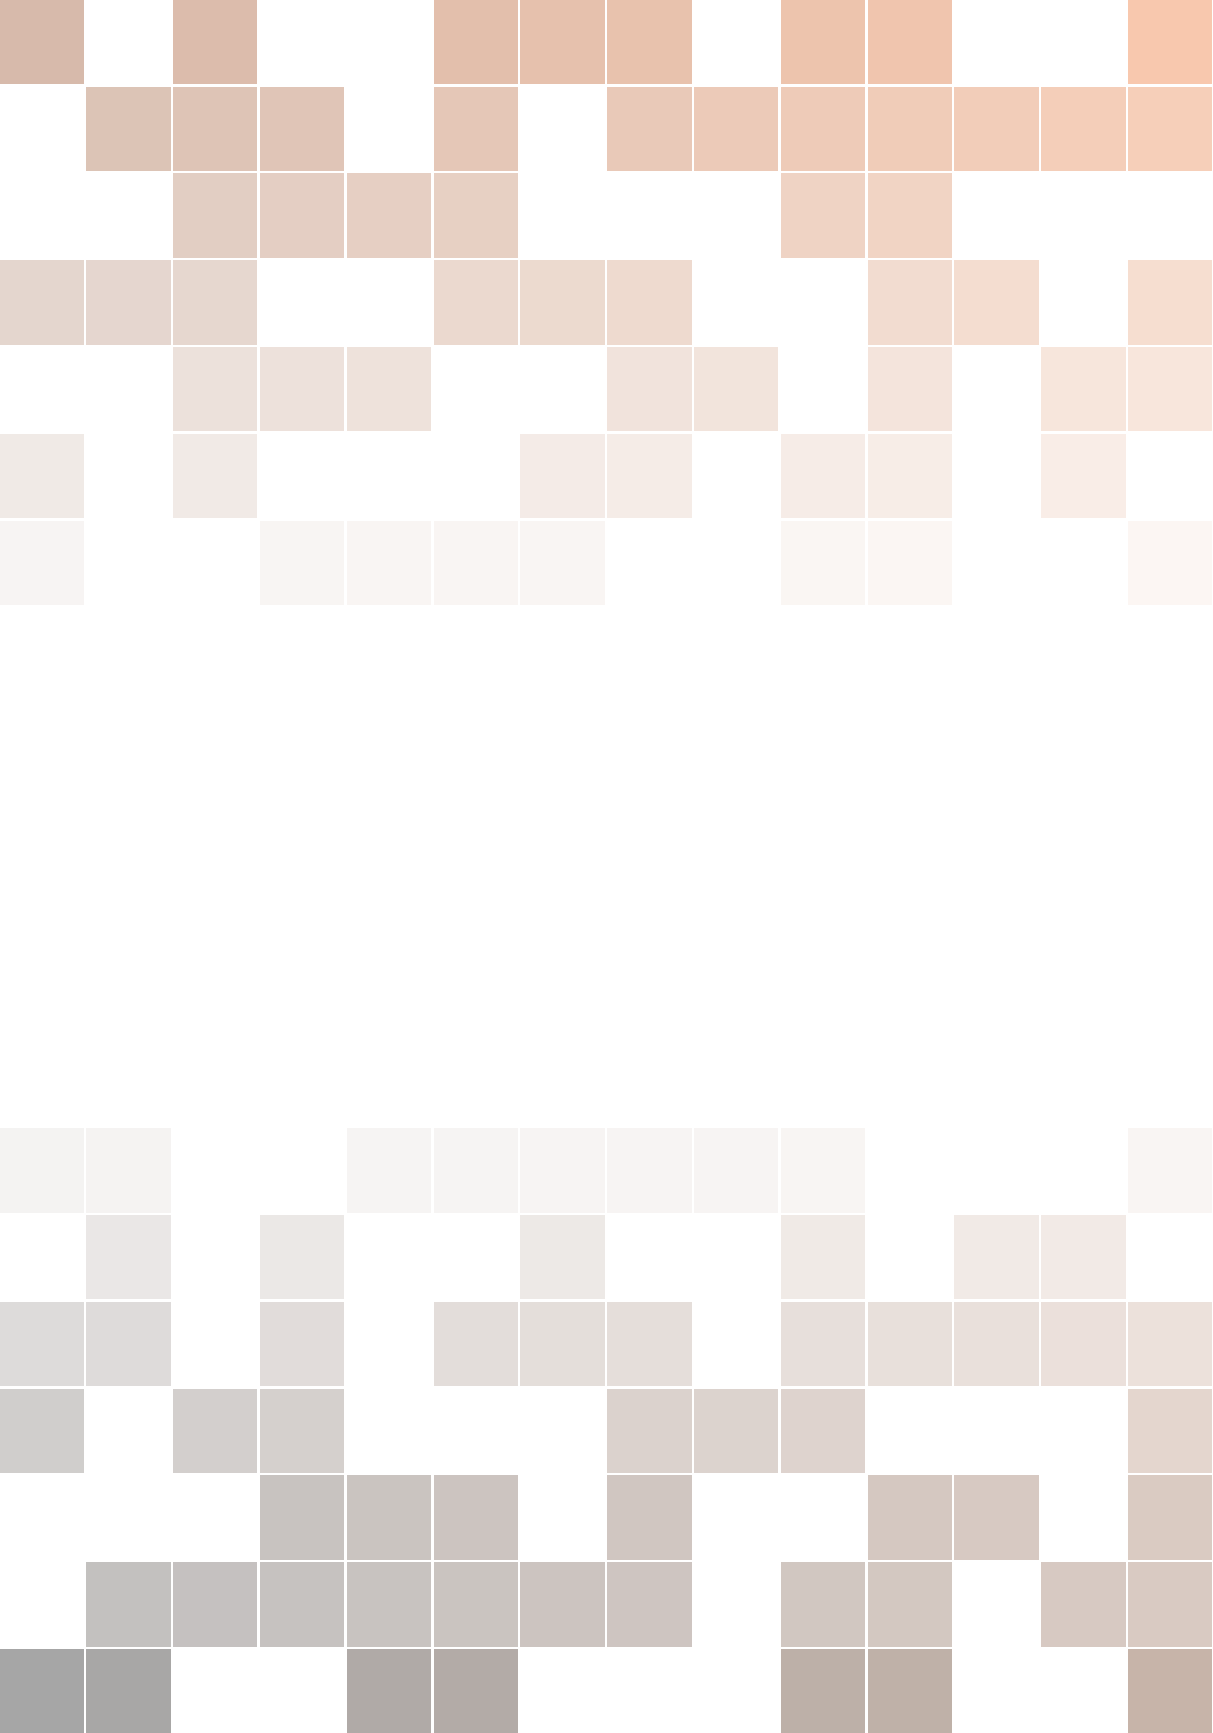
\includegraphics[width=\paperwidth]{background}};
\draw (current page.center) node [fill=ocre!30!white,fill opacity=0.6,text opacity=1,inner sep=1cm]{\Huge\centering\bfseries\sffamily\parbox[c][][t]{\paperwidth}{\centering Geoestatística\\[15pt] % Book title
{\Large Introdução aos princípios}\\[20pt] % Subtitle
{\huge David Alvarenga Drumond}}}; % Author name
\end{tikzpicture}
\vfill
\endgroup

%----------------------------------------------------------------------------------------
%	COPYRIGHT PAGE
%----------------------------------------------------------------------------------------

\newpage
\thispagestyle{empty}

\begin{center}
	\Large \bf { David Alvarenga Drumond }
\end{center}

\vspace{4.0cm}

\begin{center}
	{\LARGE \bfseries Geoestatística - Introdução aos princípios }
\end{center}
\vspace {4.0cm}
\begin{center}
	\Large 1$\^{a}$ edição
\end{center}
\vspace{8.0cm}
	
\begin{center}
	\Large {Belo horizonte}\\
	\Large {22/09/2017}
\end{center}




%%%%%%%%%%%%%%%%%%%%%%
% Ficha Catalográfica
\newpage
\thispagestyle{empty}
\null\vfill

\begin{center}
	\begin{tabular}{|p{12.5cm}|}%{p{12cm}}
		\hline
		\begin{small}
			\begin{verbatim}
			D249i	Drumond, David
			Geoestatística - Introdução aos princípios / 
			David A. Drumond. - Belo Horizonte : O Autor, 2017. 
			117 p. 
			
			ISBN: 978-85-923922-0-8
			
			
			1. Engenharia de Minas . 2. Geologia. 3. Geoestatística.
			I. Título.
		
			CDD: 550
			\end{verbatim}
		\end{small}
		\\ \hline
	\end{tabular}
\end{center}
\setcounter{page}{2} %truque para não numerar a página

\newpage
\thispagestyle{empty}
\vspace*{\fill}

{ \raggedleft
	
	
	\textit{Aos meus pais pelo eterno carinho e apoio.}
	
	~
}


\newpage
\thispagestyle{empty}
\vspace*{\fill}

{ \raggedleft
	
	
	\textit{Sempre que te perguntarem se podes fazer um trabalho, \\
		respondas que sim e te ponhas em seguida a aprender como se faz. \\
		F. Roosevelt}
	
	~
}



\newpage
\section{Introdução}

Este livro é apenas uma breve iniciação aos conceitos matemáticos e definições da geoestatística, uma área dos fenômenos estocásticos que lida com variáveis aleatórias espaciais. O objetivo desta obra é auxiliar no primeiro contato com esta disciplina, tentando demonstrar da maneira mais simples o funcionamento da teoria, primeiramente concebida por Matheron, e depois formalizada por uma gama de autores, que tornou a geoestatística uma ferramenta poderosa na avaliação de vários processos de engenharia, ciências e até mesmo medicina. No entanto, este é um livro criado principalmente para estudantes de graduação dos cursos voltados para as áreas de mineração. O primeiro capítulo envolverá uma série de conceitos sobre planejamento mineral e geologia, de forma a incluir o leitor no assunto. O segundo capítulo trata da formalização da teoria das variáveis aleatórias regionalizadas. Em seguida são introduzidos conhecimentos de estatística básica envolvendo o tratamento univariado e bivariado. Técnicas de desagrupamento são então iniciadas, demonstrando ao leitor a importância da prática de amostragem. Por conseguinte as funções de continuidade espacial e variografia são conceituadas, para então serem introduzidas as técnicas de estimativa espacial também conhecida como krigagem. Por final, o livro apresenta as curvas de teor e tonelgagem que representam um resumo final da avaliação do depósito mineral. É importante lembrar que este livro é apenas introdutório e não representa um sumário de todas as técnicas geoestatísticas possíveis. Na verdade, esta obra se limita apenas a um entendimento básico do planejamento mineral e muitas outras técnicas foram desenvolvidas para lidar com problemas multivariados ou simulação de depósitos minerais. No entanto, mesmo sendo um livro simples, ainda representa um alicerce na construção do conhecimento geoestatístico pelo leitor e muito do que ainda se pratica no meio da mineração é ainda observado com estas metodologias simples. 


\
%----------------------------------------------------------------------------------------
%	TABLE OF CONTENTS
%----------------------------------------------------------------------------------------

%\usechapterimagefalse % If you don't want to include a chapter image, use this to toggle images off - it can be enabled later with \usechapterimagetrue

\chapterimage{chapter_head_1.pdf} % Table of contents heading image

\pagestyle{empty} % No headers

\tableofcontents % Print the table of contents itself

\cleardoublepage % Forces the first chapter to start on an odd page so it's on the right

\pagestyle{fancy} % Print headers again

%----------------------------------------------------------------------------------------
%	PART
%----------------------------------------------------------------------------------------




\chapter{Introdução a geoestatística}
 
\begin{myquoting}{The art and the science of resource estimation\\Jacqui Coombes}
	A estimativa de recursos é o processo de criação de um reflexo tridimensional da mineralização \textit{in situ} baseado em amostras esparsas utilizando conhecimento geológico corrente e um caminhão carregado de senso comum.
\end{myquoting}

\section{Introdução ao capítulo} 

Este capítulo inicial pretende demonstrar os primeiros passos para entender a geoestatística. Afinal, o que é a geoestatística? Qual é o seu objeto de estudo?  O que podemos fazer ou não com a geoestatística? Para que um marceneiro possa fazer uma cadeira, por exemplo, ele precisa entender de suas ferramentas e de seu funcionamento, para que possa selecionar as mais adequadas para o seu trabalho. Entendendo o que é a geoestatística e como podemos utilizá-la, principalmente no setor da mineração, estabelecemos um vínculo necessário para a aplicação correta desta poderosa ferramenta.

\section{Afinal, o que é geoestatística?}

A importância das substâncias metálicas na indústria mineral brasileira é historicamente associado aos tempos da Colônia, procurando rotas inicialmente no estado de Minas Gerais. Segundo o relatório da Agência Nacional de Mineração (2018), a produção das principais substâncias metálicas no país atingiram um valor de 41,7 bilhões de reais em exportação.  A produção mineral rende impostos para as regiões produtoras, que ao mesmo tempo permitem o desenvolvimento da economia local e geração de empregos. A decisão da extração e produção mineral, no entanto, advém do conhecimento geológico e de estimativas dos corpos minerais aos quais muitas vezes não se possui acesso. Os corpos geológicos, muitas vezes, não apresentam informações superficiais de fácil acesso, como afloramentos que permitem a definição da \textbf{atitute} das camadas, por isso é necessário realizar amostragens em grande profundidade como na obtenção de \textbf{testemunhos de sondagem}. A partir de uma sonda são retirados fragmentos de rocha à profundidades de até 400m, permitindo que tenhamos informações da composição direta das rochas naquela região. A figura \ref{testemunho_de_sondagem} exemplifica a forma cilíndrica apresentada pelo testemunho de sondagem obtido em campanhas de pesquisa mineral.


\FloatBarrier
\begin{figure}[!htb]
	\centering
	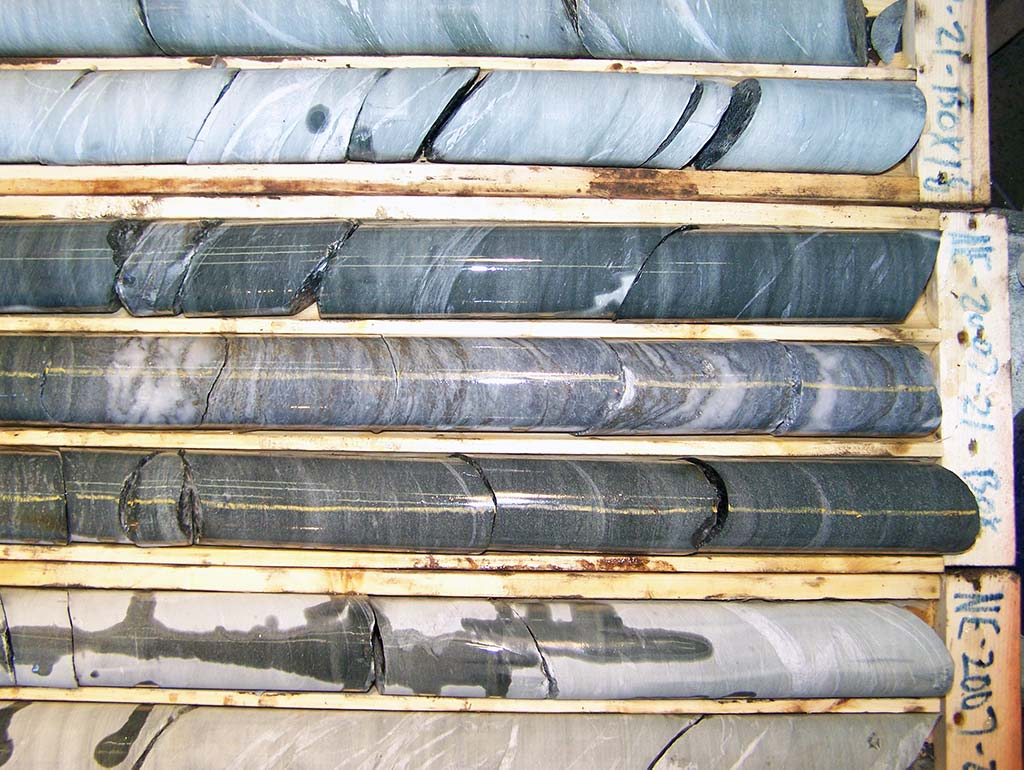
\includegraphics[width=0.8\textwidth,height=30mm]{./Capitulo_0/testemunho.jpg}	
	\caption{Testemunhos de sondagem de rochas. Amostras retiradas a partir da perfuração do solo, que apresentam uma informação contínua vertical das rochas e mineralogias presentes em uma região. }
	\label{testemunho_de_sondagem}
\end{figure}
\FloatBarrier

Desta forma, a única informação que possuímos é a informação vertical fornecida pelos testemunhos, como demonstrado na figura \ref{testemunhos_sondagem_vertical}. As decisões da mineração não podem ser estabelecidas sem o conhecimento das informações entre os furos de sondagem, que podem representar malhas espaçadas em muitos metros. A amostragem exaustiva dos depósitos minerais também é inviável economicamente, pois em alguns casos, cada metro de amostra sondada pode corresponder a um valor de \$100 a \$400 reais. 



\FloatBarrier
\begin{figure}[!htb]
	\centering
	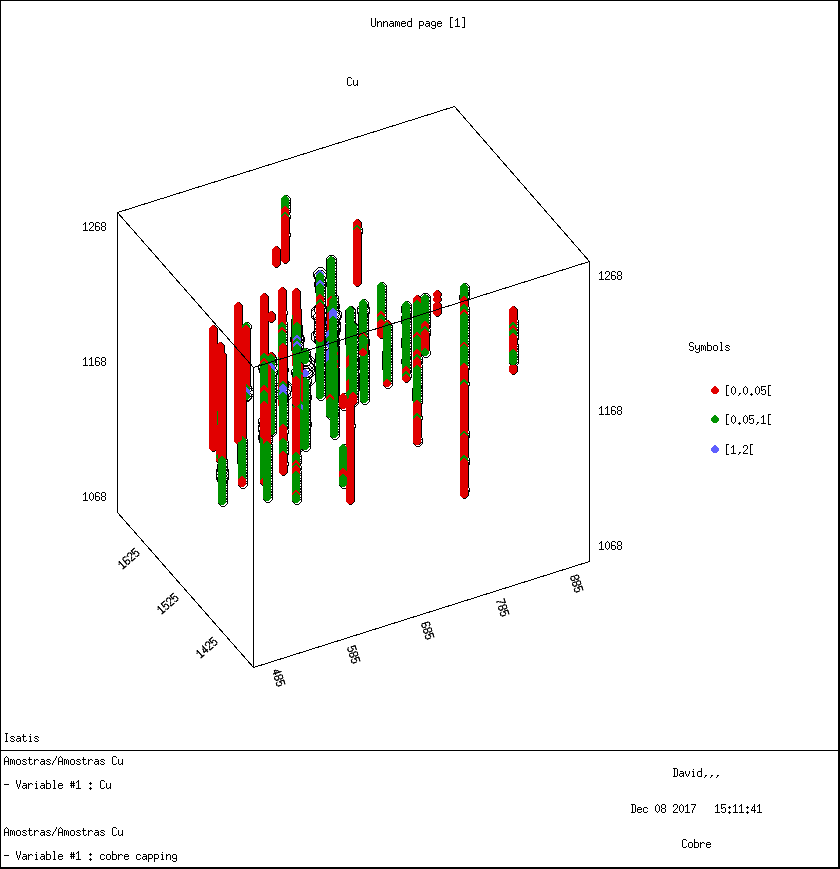
\includegraphics[scale=0.45]{./Capitulo_0/samples.png}	
	\caption{Testemunhos de sondagem representados em um software de mineração, para um depósito de cobre. }
	\label{testemunhos_sondagem_vertical}
\end{figure}
\FloatBarrier

A geoestatística é a ciência que permite a espacialização das informações obtidas em um volumes menores, para um domínio maior, de forma a permitir o planejamento e tomada de decisões na mineração, e o estudo sistemático dos corpos mineralizados. A figura \ref{simulado_teste} demonstra a espacialização dos dados obtidos na figura \ref{testemunhos_sondagem_vertical} dos testemunhos de sondagem de cobre.

\FloatBarrier
\begin{figure}[!htb]
	\centering
	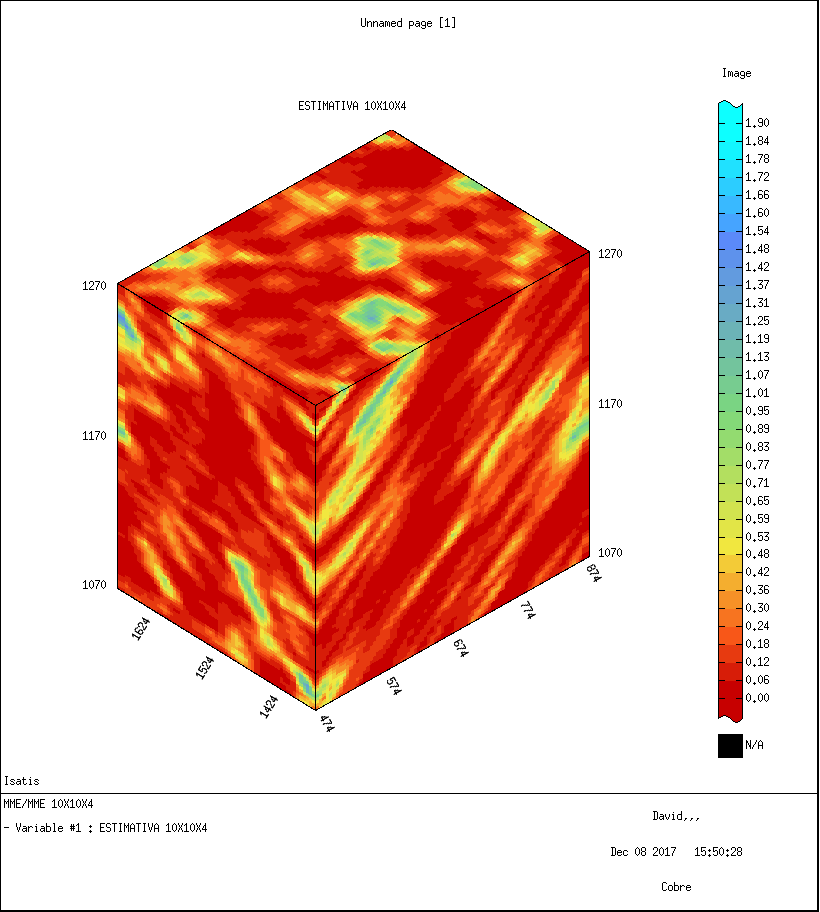
\includegraphics[scale=0.45]{./Capitulo_0/simulado.png}	
	\caption{Espacialização a partir das amostras do testemunho de sondagem obtidos na figura \ref{testemunhos_sondagem_vertical}, para um depósito de cobre. }
	\label{simulado_teste}
\end{figure}
\FloatBarrier

 A partir de um modelo espacializado é possível planejar a mineração e tomar a decisões na lavra, como a criação de \textbf{modelos econômicos}, a determinação das \textbf{cavas matemáticas}, o \textbf{sequenciamento das operações}. Segundo \citet{rossi2013mineral}, o objetivo principal da geoestatística consiste em 4 etapas principais: 
 
 \begin{enumerate}
 	\item Obtenção de amostras e administração da amostragem
 	\item Interpretação geológica e modelagem 
 	\item Interpolação dos teores
 	\item Acesso às incertezas geológicas
 \end{enumerate}

A \textbf{obtenção de amostras e administração da amostragem} consiste no conjunto de técnicas utilizada para obter uma malha de amostragem que reduza o erro obtido pela interpolação espacial das propriedades de interesse. Por exemplo, a malha de amostragem em um depósito de ferro bandado, conhecido como \textit{(Banded Iron Formations)} , pode ser dimensionada para que se reconheçam os minerais deletérios durante a fase de metalurgia. 

A \textbf{interpretação geológica e modelagem} permite reconhecer as dimensões e formas do corpo geológico e principais estruturas. Um dos grandes desafios da mineração é conseguir reconhecer os limites dos corpos minerais e sua forma. A geoestatística permite utilizar técnicas que auxiliem no reconhecimento das formas destes corpos de maneira grosseira, a partir da \textit{modelagem implícita}. O objetivo do uso destas técnicas é reduzir a quantidade de trabalho demandada pelo geólogo para que se possam produzir modelos condizentes com a realidade, e ao mesmo tempo, poupar trabalho excessivo pelo desenvolvimento de seções verticais. 

A \textbf{Interpolação de teores} consiste no objetivo principal deste livro, em que realizamos a espacialização das propriedades de interesse das amostras para um domínio espacial maior. Esta espacialização pode ser realizada para apenas uma variável (caso univariado), ou para diversas variáveis em conjunto (caso multivariado). O objetivo principal da interpolação é garantir, com maior segurança possível, que um volume direcionado da lavra para o beneficiamento mineral possua \textbf{valor esperado}, ou \textbf{valor médio}, correto. 

O \textbf{Acesso às incertezas geológicas}  pode ser realizado a partir de técnicas avançadas de geoestatística como a simulação, ou geoestatística não-linear. Pretende-se desta forma tentar reconhecer as incertezas locais de uma propriedade do depósito, e avaliar quão díspares podem ser as medições em regiões do depósito que desconhecemos. A incerteza geológica é, sem dúvida, um dos fatores que mais afetam o \textbf{risco} do empreendimento mineiro. Para que os investidores possam verificar o risco de seus investimentos, foram criados os \textbf{códigos de mineração}, que criaram padrões nomear regiões do depósito mineral com maior ou menor incerteza quanto uma propriedade de interesse, geralmente aquela de retorno econômico. 
 
 Segundo \citet{matheron1963principles}, criador da geoestatística, podemos definí-la tal como:
 
 \FloatBarrier
 \begin{remark}	
 	\textit{"Geoestatística, na sua maior aceitação, consiste no estudo da distribuição do espaço de valores úteis para engenheiros de minas e geólogos, como teores, espessura da camada, ou acumulação, incluindo as práticas mais importantes para a avaliação de depósitos minerais" - \cite{matheron1963principles}} 
 \end{remark}
\FloatBarrier

Atualmente o uso da geoestatística compreende uma diversidade enorme de áreas, desde a \textbf{engenharia civil}, \textbf{engenharia agrícola}, \textbf{engenharia ambiental}, \textbf{geografia}, \textbf{engenharia hídrica} e até mesmo em áreas que não se resumem à dados geograficamente referenciados, mas espacialmente referenciados em objetos ou seres, como a \textbf{mecânica} ou \textbf{medicina}. Podemos entender a geoestatística sob uma perspectiva mais ampla, abordando o estudo das incertezas a cerca de fenômenos temporalmente ou espacialmente localizados. O professor \citet{goovaerts1997geostatistics}, demonstra claramente a nossa dificuldade de entender as incertezas:

 \FloatBarrier
\begin{remark}	
	\textit{"A respeito da incerteza ... ela surge do nosso conhecimento imperfeito do fenômeno, dependente dos dados e ainda mais dependente do modelo, em que o modelo especifica nossas decisões (concepções) a priori do fenômeno. Nenhum modelo tal como a medida da incerteza, pode ser objetiva." - \cite{goovaerts1997geostatistics}} 
\end{remark}
\FloatBarrier

Podemos entender então as limitações acerca dos modelos geoestatísticos. Estamos sempre \textbf{dependentes das amostras recolhidas para a avaliação}, como também a escolha dos modelos que melhor representam as características de um fenômeno. A geoestatística constitui atualmente a área que melhor consegue caracterizar a incerteza geológica, dada as condições de amostragem que obtemos na mineração e de muitos problemas georeferenciados.  Definimos a geoestatística como:

\begin{definition} [Geoestatística]
	\textit{A geoestatística é a ciência capaz de transformar as informações obtidas por amostras georeferenciadas em conhecimento, a partir da caracterização da incerteza geológica, da interpretação destes dados, das inferências e estimativas, e da tomada de decisão pelo reconhecimento do fenômeno estudado.}
\end{definition}

 \section{Qual é o objeto de estudo da geoestatística?}
 
 A geoestatística é a ciência que permite o estudo de variáveis regionalizadas. O capítulo \ref{cap_var_reg} trará informações a respeito desta teoria, que compõe o objeto principal do estudo da geoestatística. Uma variável regionalizada é aquela que pode assumir um valor específico no espaço. Este valor é \textbf{determinístico}, gerado a partir de fenômenos que muitas vezes não conhecemos. Por não conseguirmos acessar as informações a respeito desta variável, optamos por utilizar uma metodologia \textbf{estocástica} para acessar a nossa \textbf{incerteza} a cerca do fenômeno que estudamos. Desta forma pensamos na variável regionalizada com um aspecto \textbf{dicotômico}, a medida que possui valor real onde conhecemos, e valor aleatório onde desconhecemos. 
 
 O físico Erwin Schrödinger desenvolveu um problema em 1935 muito similar a esta condição das variáveis regionalizadas. O experimento foi chamado de "Gato de Schrödinger". O experimento propunha que um gato fosse preso em uma caixa, com um veneno que poderia aleatoriamente ser liberado, matando o gato em seguida. Para quem observa a experiência do lado de fora, não há como detectar se o gato está vivo ou morto, logo o estado de sobrevivência do gato é indefinido, dependendo da real observação de dentro da caixa. A figura \ref{gato} demonstra este experimento. 
 
 
 \FloatBarrier
 \begin{figure}[!htb]
 	\centering
 	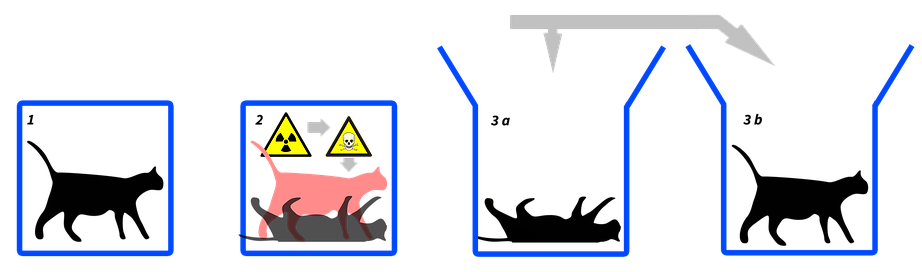
\includegraphics[scale=0.60]{./Capitulo_0/gato.png}	
 	\caption{Experiência do "Gato de Schrödinger", proposta em 1935 pelo físico Austríaco Erwin Schrödinger. 1) O gato está dentro da caixa, 2) Passado um tempo o observador externo não sabe o que está dentro da caixa. 3a) Abre-se a caixa e define-se que o gato está morto. 3) Abre-se a caixa e define-se que o gato está vivo.  }
 	\label{gato}
 \end{figure}
 \FloatBarrier
 
 Quando pensamos em termos da mineração, o problema de se definir minério ou estéril é similar ao do "Gato de Schrödinger". Não sabemos de fato o que será minerado deve ser enviado para o beneficiamento mineral, a não ser que de fato retirarmos o material do local. As \textbf{variáveis regionalizadas} funcionam de forma bem semelhante, possuindo este aspecto ao mesmo tempo determinístico e aleatório. Um depósito mineral é um evento geológico realizado durante milhões de anos. Durante o tempo de existência humana é quase impossível que estes depósitos minerais se modifiquem. Desta forma o corpo mineral, ou o "gato" já está dentro da caixa há muito tempo, porém nos é impossível determinar o seu atual estado sem que ocorra a mineração. 
 
 Ao estudar as variáveis regionalizadas, a  geoestatística propõe encontrar valores e relações que desconhecemos, sem obtermos informações diretas do depósito mineral. Considerando a variabilidade inerente destas variáveis podemos criar modelos estatísticos que possam inferir propriedades que desconhecemos em outras regiões do depósito mineral.
  

 \section{O que podemos fazer com a geoestatística?}
 
 A partir da avaliação dos depósitos minerais utilizando a geoestatística, podemos caracterizar o fenômeno espacial e quantificar as incertezas para diferentes \textbf{variáveis}. Uma variável é uma característica  de interesse de estudo no depósito mineral, que se modifica segundo seu posicionamento no espaço. No estudo da mineração possuímos uma série de diferentes tipos de variáveis associadas ao depósito mineral, tais como:
 
 \begin{enumerate}
 	\item \textbf{Químicas}: Teores de elementos químicos de interesse, ou de elementos deletérios prejudiciais no processamento mineral
 	\item \textbf{Físicas}: Dureza, densidade, condutibilidade térmica, condutibilidade hidráulica, saturação
 	\item \textbf{Geológicas}: Litologia, composição mineralógica, número de falhas, RQD (Rock quality index)
 	\item \textbf{Processamento}: Recuperação metalúrgica, recuperação mássica, moabilidade, consumo de reagentes
 	\item \textbf{Operacionais}: Resistência a penetração, consumo de explosivos, tempo de carregamento 
 	\item \textbf{Econômicas}: Preço de mercado, valor presente líquido
 \end{enumerate} 

O entendimento de cada uma destas variáveis permite a tomada de decisão de lavra de uma parte constituinte do depósito mineral. O uso de modelos geoestatísticos para cada uma destas variáveis deve, no entanto, ser específico para cada tipo de variável calculada. Neste livro introdutório abordamos principalmente os problemas que se relacionam com variáveis consideradas \textbf{aditivas}. Algumas variáveis que podem ser consideradas aditivas, e que representam o maior escopo de trabalho dos avaliadores de depósito mineral são \textbf{teor do elemento metálico}, \textbf{quantidade de metal de interesse}, \textbf{massa do minério} e \textbf{acumulação}. \citet{carrasco2008additivity} demonstra o conceito de aditividade de variáveis, expresso por: 


\FloatBarrier
\begin{remark}	
	\textit{"Quantidades consideradas aditivas são aquelas que a quantidade média é igual a média das quantidades." - \cite{carrasco2008additivity}} 
\end{remark}
\FloatBarrier

A variável teor, por exemplo, pode ser considerada uma variável aditiva, pois a média aritmética dos teores de duas regiões de mesma forma e volume é idêntico ao valor médio do teor nestas regiões. No caso da recuperação metalúrgica, por exemplo, não há possibilidade de se considerar a média aritmética como valor médio, sendo impossível utilizar a geoestatística linear para estimar valores de recuperação metalúrgica. \citet{carrasco2008additivity} ainda afirma a necessidade de variáveis aditivas para se realizar o processo de estimativa diretamente por meio da geoestatística linear clássica. 

\FloatBarrier
\begin{remark}	
	\textit{"Uma quantidade dita não aditiva, não pode modelar sua variabilidade espacial ou estimar diretamente" - \cite{carrasco2008additivity}} 
\end{remark}
\FloatBarrier

Para estimar ou avaliar variáveis ditas não-aditivas recorremos aos métodos de \textbf{geoestatística não linear} ou \textbf{simulação geoestatística}. Estes métodos não serão abordados neste volume deste livro, apenas abordaremos os conceitos primários da \textit{geoestatística linear}, que envolvem o tratamento de variáveis aditivas. No entanto, para o leitor iniciante, é importante entender que os métodos deste livro apenas se aplicam para \textbf{variáveis aditivas} e para amostra com o mesmo volume e forma, conceito denominado de \textbf{suporte amostral}. As estimativas realizadas no depósito mineral geralmente são feitas em volumes maiores, chamado de \textbf{suporte da estimativa} e compõe a chamada \textbf{unidade seletiva de lavra}. Segundo \citet{rossi2013mineral} uma unidade seletiva de lavra pode ser caracterizada como:

\FloatBarrier
\begin{remark}	
	\textit{"Mínimo volume de material ao qual o minério e o estéril podem ser separados, em função do método de lavra e da seletividade" - \cite{rossi2013mineral}} 
\end{remark}
\FloatBarrier

Podemos então discretizar o espaço em pequenos blocos, para se realizar a estimativa nestes locais. Este é chamado de \textbf{modelo de blocos}, representado na figura \ref{mod_blok}.

\FloatBarrier
\begin{figure}[!htb]
	\centering
	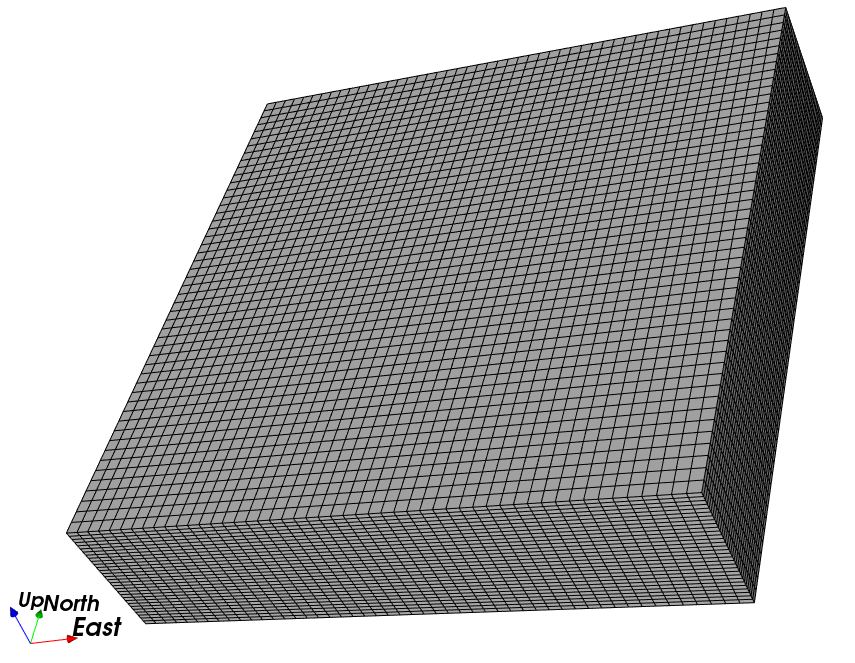
\includegraphics[scale=0.30]{./Capitulo_0/modelo_bloco.png}	
	\caption{Representação de um modelo de blocos e discretização do espaço. }
	\label{mod_blok}
\end{figure}
\FloatBarrier

Assim podemos dividir o espaço a ser estimado em pequenos volumes de decisão na lavra. Para fins de planejamento mineral, quanto menor o tamanho destes blocos, melhor a facilidade do planejamento. No entanto, para fins de avaliação de depósitos, blocos de tamanho pequeno produzem estimativas espúrias. 

O equilíbrio entre estas duas vontades deve ser encontrado para constituir o tamanho adequado da unidade seletiva de lavra. Uma das regras de ouro da mineração geralmente afirma que: \textbf{o tamanho do bloco não deve ser inferior a 1/4 do tamanho da malha de amostragem}. Esta é uma afirmação atrela o tamanho do bloco geralmente a uma malha de amostragem bem definida e calculada, o que muitas vezes não condiz com as questões práticas.

\begin{proposition}
	\textit{Segundo a regra de ouro da geoestatística um bloco estimado não deve ter tamanho inferior a 1/4 do espaçamento da malha de amostragem. Quando considerada uma malha irregular este tamanho não pode ser menor que 1/4 do valor esperado dos espaçamentos. O valor esperado pode ser calculado a partir da média aritmética dos espaçamentos.}
\end{proposition}

A discretização do depósito mineral em diferentes domínios nem sempre ocorre somente em modelos de blocos. Diferentes formas de caracterização dos volumes no espaço pode ser utilizada na geoestatística e no planejamento minera. A Figura \eqref{Modelo_blocos} demonstra alguns exemplos de divisão do espaço. Algumas delas como \textbf{polígonos de influência} e \textbf{triangulação de Delunay} representam antigas formas de estimativa de um depósito mineral, mas que, no entanto, ainda são usuais por outras formas de análise. 

\FloatBarrier
\begin{figure}[!htb]
	\centering
	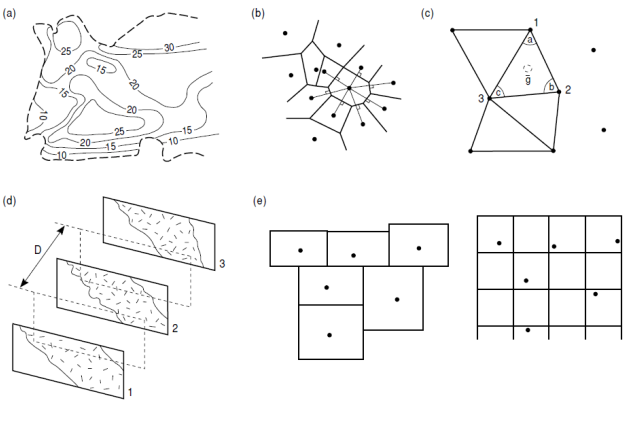
\includegraphics[scale=0.6]{./Capitulo_0/Modelo_de_blocos.png}	
	\caption{Figura demonstrando diversas apresentações de uma propriedade do depósito mineral. a) isolinhas b) Polígonos de influência c) triangulação d) seção paralelas e) blocos irregulares f) blocos regulares }
	\label{Modelo_blocos}
\end{figure}
\FloatBarrier

A partir da definição das variáveis do depósito mineral o engenheiro é capaz de estimar a viabilidade técnica e econômica do depósito mineral.  O artigo 6, do decreto 9.406 de 12 de junho de 2018 do código mineral vigente define:

\begin{definition}[Jazida Mineral]
	\textit{Toda a massa de substância mineral ou fóssil, que aflore na superfície ou já exista no solo, no subsolo, no leito ou no subsolo do mar territorial, da zona econômica exclusiva ou da plataforma continental, que tenha valor econômico}
\end{definition}


 A partir da avaliação de depósitos minerais, conseguimos então, identificar regiões econômicas e capazes do aproveitamento industrial. 


\section{Como utilizar a geoestatística?}

A geoestatística clássica utilizada neste livro não aborda conceitos matemáticos complexos, mas ainda sim constitui base para a resolução de muitos problemas de estimativa na mineração. Mesmo que os cálculos não sejam complexos, são de certa forma muito onerosos computacionalmente. As resoluções podem ser demoradas e alguns casos exigirem alta performance computacional. Desta forma, o uso de algoritmos refinados se torna cada vez mais importante nas análises geoestatísticas. 

Durante a fase de avaliação das jazidas minerais o computador exerce função essencial como ferramenta de estudo. Uma quantidade substancial de softwares estão disponíveis em meio comercial e alguns aplicativos livres também existem. Softwares comerciais são mais custosos, mas possuem suporte técnico e manutenção de seus sistemas. Apresentam código fechado ao público externo e pertencente geralmente aos proprietários. Softwares gratuitos geralmente são disponibilizados por universidades, possuem código aberto ao público e podem ser facilmente obtidos via Internet. 

Uma das bibliotecas gratuitas mais importantes é sem dúvida o GSLIB (Geostatistical Software Library) e apresenta além dos executáveis do programa seus algoritmos, escritos em Fortran 90 e disponibilizados no site. Os programas são administrados pelo doutor Clayton Deutsch e Emmanuel Schnetzler. Mais informações sobre o pacote de softwares pode ser encontrado no site \url{www.gslib.com} ou no guia de uso \cite{deutschcv1998gslib}. Neste livro abordamos nas seções A, B e C o uso dos principais softwares e linguagem R.  

O alinhamento da geoestatística com o desenvolvimento de algoritmos cria dependências com as disciplinas de programação. Os engenheiros e geólogos estão cada vez mais alinhados com o desenvolvimento de algoritmos, principalmente com as linguagem R e Python, pela sua simplicidade e facilidade de implementação.

O uso dos softwares de mineração geralmente requerem que os arquivos de dados sejam organizados eficientemente em formatos pré-estabelecidos, gerados pelas campanhas de exploração.  Essa compilação dos dados é trabalhosa e necessita de uma validação primordial, tornando o trabalho de preparação dos dados às vezes muito mais demorado que as implementações dos programas.  

Entre as aplicações mais comuns encontradas em softwares de mineração, temos:

\begin{itemize}
\item Uma grande variedade de procedimentos de avaliação dos dados (estatísticas, gráficos, etc.:)
\item Determinação da qualidade dos dados e dos protocolos de amostragem
\item Modelagem tridimensional e visualização de formas geológicas complexas e distribuição das amostras.
\item Preparação de seções planas e verticais 
\item Gráficos de contorno tanto do teor como de outras variáveis 
\item Caracterização da continuidade espacial (Variogramas automáticos, mapas de variograma, variogramas experimentais e modelagem)
\item Modelagem de blocos do depósito
\item Metodologias de cálculos de recurso e reservas
\item Avaliações dos efeitos de vários métodos de mineração
\item Determinação da viabilidade econômica de depósitos
\end{itemize}

Alguns destes softwares podem ainda incluir ferramentas de planejamento de mina, tal como otimização de cava, sequenciamento, desenho de cava, etc. A grande quantidade de ferramentas adicionadas nestes programas geralmente os tornam pouco específicos para análises espaciais, obtendo apenas algumas rotinas específicas para trabalhos mais simples. 


\section{O que a geoestatística não faz?} 

Toda ferramenta possui suas limitações. A geoestatística é a melhor ferramenta para análises espaciais até então criada, mas ela possui limitações no uso de seus modelos. Primeiramente \textbf{a geoestatística não é uma caixa preta}. Isso significa que uma boa análise do depósito mineral não depende exclusivamente de apertar um botão, como muitos modelos mais simples fazem. Para criar modelos geoestatísticos adequados eles devem passar por uma intensa avaliação e reavaliação dos parâmetros de ajuste destes modelos. 

Em segundo lugar \textbf{a geoestatística não é uma bola de cristal}. Quando realizamos estimativas estamos susceptíveis a erros e incertezas. Uma boa estimativa dos depósitos minerais propiciará redução dos erros, mas inevitavelmente não podemos sempre esperar resultados exatos. Além das condições relacionadas a escolha e refinamento dos modelos, também temos condições inerentes da incerteza geológica.  \citet{maranhao1985introduccao} demonstra a classificação de jazidas minerais no ponto de vista da avaliação de reservas, identificando quatro grupos principais: 

\begin{enumerate}
	\item \textbf{Grupo 1}. Pertence aos depósitos estratiformes, cujos representantes típicos são as jazidas sedimentares de origem marinha, que possuem grandes dimensões, forma mais ou menos constante, e regularidade na distribuição de teores.  Também  incluem neste grupo as jazidas metamórficas de ferro, tais como nos depósitos do quadrilátero ferrífero. Também apresenta alguns depósitos de disposição horizontal ou a subhorizontal como jazidas de calcário, carvão, sais, gipsita e alguns depósitos para construção civil, como gnaisses e granitos.
	\item \textbf{Grupo 2}. O segundo grupo apresenta corpos minerais interrompidos ou levemente interrompidos e uma distribuição mais irregular dos teores que do primeiro grupo. Estas representam as jazidas de alteração superficial como depósitos de níquel e bauxita, depósitos com pequenas intrusões alcalinas, como carbonatitos e sienitos, jazidas de rochas ultrabásicas e hidrotermais.
	\item \textbf{Grupo 3} O terceiro grupo geralmente enquadra jazidas de forma variável e mineralização muito irregular, compondo os principais depósitos auríferos, platinoides e diamantes. Também aborda os depósitos de veios polimetálicos e depósitos de forma lenticular, como de cobre e níquel. 
	\item \textbf{Grupo 4} Representa o grupo mais irregular de todos, compondo pegmatitos de pedras preciosas, alguns veios hidrotermais com metais raros e nobres e algumas jazidas ultrabásicas de platina e diamante. 
\end{enumerate}

Quanto maior a irregularidade do depósito e heterogeneidade de suas propriedades, maior será a dificuldade dos modelos geoestatísticos de predizerem com exatidão os resultados. Dependendo da \textbf{continuidade espacial} da propriedade e da sua \textbf{dispersão}, a aplicação de modelos simples ou complexos simplesmente não altera o nosso conhecimento sobre a \textbf{incerteza geológica}, pois a complexidade do depósito mineral é tão grande, e as amostragens realizadas em tão pouca quantidade, que se torna mais fácil jogar uma moeda para cima para decidir se devemos ou não lavrar um depósito. Neste caso, quando os métodos geoestatísticos falham, é necessário rever as metodologias de amostragem, e tentar encontrar soluções que simplifiquem as variáveis do problema. 

Desta forma a geoestatística também tem outra limitação: \textbf{Os modelos geoestatísticos requerem amostras realizadas em quantidade e qualidade adequada para gerar resultados satisfatórios}. Esta talvez seja uma das limitações mais difíceis de se conseguir abordar dentro da mineração. Para estimar de forma adequada precisa-se de amostras, e amostras são caras. Muitas empresas deixam de amostrar adequadamente seus depósitos minerais com finalidade de redução de custos, mas acabam por avaliar mal seus depósitos minerais, e consequentemente, obtém baixo lucro ou inviabilizam o uso sustentável dos recursos minerais. O termo qualidade, também é uma questão muito importante. Muitas vezes as amostragens realizadas possuem protocolos mal dimensionados. Alguns métodos de amostragem de jazidas também devem ser conduzidos de forma bem precisa para realizarem estimativas adequadas, mas apesar de ser uma das etapas mais importantes na mineração, as empresas muitas vezes colocam a tarefa nas mãos de profissionais pouco qualificados. 


\section{Questões éticas na avaliação de depósitos minerais} 

Avaliar depósitos minerais é uma atividade incerta, devido a natureza dos depósitos minerais, no entanto, não há justificativa para o mal uso das técnicas, nem ao mesmo para decisões arbitrárias que não envolvam decisões puramente lógicas ou racionais. Infelizmente o setor mineral acaba por ser alvo de pessoas com má conduta, por ser uma área de grandes riquezas. Esta não é, com certeza, a personalidade da grande maioria dos trabalhadores que se dedicam diariamente no setor mineral, mas pessoas acabam por utilizar a justificativa do "incerto" para vender depósitos minerais subvalorizados. Um avaliador de depósitos minerais deve realizar sua tarefa friamente, analisando a viabilidade do depósito independente se ele gerará riquezas ou não. 

É importante também para os gestores e gerentes de minas entenderem a natureza do problema, e que as incertezas geológicas produzirão muitas vezes resultados diferentes dos pretendidos. A mineração trata do aproveitamento de recursos que são limitados pelo tempo geológico de sua criação. Enquanto o ser humano ainda não controlar o tempo, é indiscutível que temos de aproveitar os recursos minerais existentes da melhor forma que consigamos. A avaliação de depósitos minerais é o alicerce das decisões na mineração, por isso é impreterível que os processos sejam realizados de forma mais correta possível. 

\begin{proposition}
	\textit{Está nas mãos do avaliador de depósitos minerais a determinação das condições necessárias para a progressão da lavra. O desenvolvimento de seus projetos deve seguir sempre com conhecimento e idoneidade, pois é dele que deriva o trabalho de pessoas, o aproveitamento correto dos recursos minerais e da sociedade que aproveita estes recursos}
\end{proposition}

\section{Alguns conceitos iniciais sobre jazidas minerais}

Apresentamos nesta seção alguns dos principais conceitos de engenharia de minas, necessários para a realização de trabalhos de geoestatística e avaliação de depósitos no setor mineral. Apesar deste livro possuir foco na geoestatística, consideramos adequado entender conceitos gerais da mineração, que influenciam nas decisões tomadas pela avaliação dos depósitos.

\subsection{Minério} 

A definição de minério talvez seja uma das mais importantes na produção mineral. A sua determinação permite o aproveitamento econômico dos recursos minerais, decidindo o que deve ou não ser lavrado e aproveitado. Segundo \citet{hustrulid2006open}, a definição de minério pode ser considerada como:

\begin{remark}
	\textit{"Um agregado mineral com um ou mais sólidos minerais aos quais podem ser minerados, ou dos quais um ou mais produtos minerais podem ser extraídos com lucro".  \citet{hustrulid2006open}}
\end{remark}

Isto significa que nem em todas as ocasiões um minério será extraído com a finalidade de se obter lucro pela venda. Em alguns casos, as questões econômicas da extração mineral podem ser contra intuitivas neste sentido, devido a políticas externas, estados de guerra, monopolização da produção, entre diversos outros fatores. Neste caso preferimos adotar o conceito de minério a partir do seu benefício, nem sempre ele sendo econômico. Definimos minério como: 

\begin{definition}[Minério]
	\textit{Minério é todo agregado mineral ou fóssil cabível de aproveitamento técnico, que possibilita um benefício, seja ele econômico ou social, de forma a propiciar os interesses das diferentes componentes da sociedade, sejam elas a União, as forças sociais ou mineradores.}
\end{definition}

Um exemplo bem característico de minérios explotados contra o senso econômico são os minerais radioativos, de monopólio da União. É de interesse estratégico de um país deter estes recursos capazes de produzir energia e armas, sendo muitas vezes gastos valores acima do valor do minério para sua extração. 


\subsection{Teor de corte e teor crítico}

O conceito de teor de corte (ou cutoff) é definido como aquele em que o valor do conteúdo metálico ou mineral, em um certo volume de rocha, permite sua extração econômica. Os teores de corte são usados para distinguir blocos de minério e estéril em vários estágios da evolução da estimativa da jazida mineral (exploração, desenvolvimento e produção). O teor crítico, no entanto, representa o teor ao qual se delimita o limite entre prejuízo e lucro. \citet{rendu2014introduction} define o teor de corte como:


\begin{remark}
	\textit{"O teor de corte geralmente é definido como a mínima quantidade de um produto de valor ou metal que em uma tonelada métrica deve conter para que este material seja enviado para a planta de beneficiamento"} - \cite{rendu2014introduction}
\end{remark}

\subsection{Continuidade}

A continuidade é um termo derivado em toda a história da matemática e da ciência desde tempos remotos. Talvez uma das primeiras concepções da continuidade seja com o pardoxo de Zenão, que conta a história da corrida de Aquiles e a tartaruga. \citet{srivastava1989robust} demonstram o sentido da continuidade como: 

\begin{remark}
	\textit{"Uma descrição da similaridade ou da dissimilaridade entre pares de valores com uma função de sua speração do vetor h"} - \cite{srivastava1989robust}
\end{remark}

Em outras palavras podemos dizer que a continuidade espacial é representada pela similaridade entre medidas que se localizam em regiões diferentes no espaço. Os fenômenos geólogicos, neste caso, apresentam uma importante característica derivada de suas gêneses: Na maioria dos casos, medidas de propriedades realizadas mais próximas tendem a ser mais similares entre si do que medidas realizadas em grandes distâncias. Caracterizar a similaridade dos fenômenos geológicos é a chave para garantir que as estimativas e a caracterização da incerteza geológicas possam ser realizadas. 

\begin{definition}[Continuidade espacial]
	\textit{Definimos a continuidade espacial como a regularidade com que uma propriedade é medida em amostras aproximadas no espaço. Se as diferenças entre as amostras for pequena, dizemos que o material é contínuo ou similar. Quando o material é muito diferente de amostras pouco espaçadas dizemos que ele é discreto ou dissimilar. Na geoestatística definimos a continuidade a partir de uma direção do espaço, podendo ela se apresentar diferencialmente de acordo com a direção adotada.}
\end{definition}

\subsection{Diluição}

Segundo \citet{susaeta2008dilution} a diluição se refere ao estéril que não é separado do minério durante a operação da lavra. Este estéril é misturado com o minério e enviado para a usina de beneficiamento. Enquanto aumenta  a quantidade de material enviado para a usina a diluição diminui o teor que deveria ser estimado e enviado para a usina corretamente. A estimativa de depósitos minerais é realizada desconsiderando os efeitos de produção e planejamento. Isto significa que os valores realmente lavrados não correspondem aos volumes planejados e induzem diferenças naturais da estimativa. O processo de comparação entre os valores reais obtidos na usina e os valores estimados pode ser definido como \textbf{aderência do planejamento de lavra} 

\begin{definition}[Aderência de lavra]
	\textit{Aderência do planejamento de lavra é todo o processo de comparação entre os valores estimados do depósito mineral e os obtidos durante a operação, seja durante a mineração, ou dos valores obtidos durante o beneficiamento mineral.} 
\end{definition}

As incertezas geológicas presentes no depósito mineral, ou as diferenças do planejamento da operação podem trazer discordâncias quanto os volumes e qualidade do material estimado e realmente lavrado, causando diluição do minério. Existem diferentes tipos de diluição durante a extração mineral. A \textbf{diluição interna} ocorre quando existem partes de estéril dentro do volume estimado do minério. Algumas vezes a amostragem pode não computar veios ou lentes de estéril dentro do bloco de decisão de lavra, dado que o volume das amostra é muito inferior ao volume das amostras. A \textbf{diluição externa} ocorre quando o planejamento mineral aborda parte do material não definido como minério, o que é comum nas regiões de contato do corpo geológico. Também há a chamada \textbf{diluição operacional}, que ocorre quando o desmonte de rochas realiza a fragmentação em regiões acima do planejado ,chamado de \textit{overbreak}, ou abaixo do planejado, chamado de \textit{underbreak}.

\subsection{Recursos e reservas minerais}

A definição de recursos e reservas minerais são alternativas para publicidade de declarações públicas relativo às incertezas geológicas do depósito mineral. A CBRR (Comissão Brasileira de Recursos e Reservas) identifica a declaração pública como:

\begin{definition}[Declaração pública]
	\textit{Declarações públicas são preparadas para informar investidores ou potenciais investidores e seus conselheiros sobre os resultados da exploração, recursos minerais ou reservas minerais. Elas incluem, mas não se limitam, a relatórios anuais ou trimestrais das entidades, notas  à imprensa, memorandos informativos, documentos técnicos, publicações em website e apresentações públicas.} 
\end{definition}

A partir de declarações públicas, as empresas podem indicar os volumes de metais e de massas estimados com base no conhecimento da incerteza geológica. Esta alternativa foi criada na década de 70, principalmente após o escândalo da empresa Bre-X, após constatado salgamento das minas de ouro em Busang na Indonésia. Definindo \textbf{Recursos} e \textbf{Reservas} minerais, o minerador classifica seus potenciais de produção segundo a incerteza geológica. A CBRR também define Recurso Mineral como:

\begin{definition}[Recurso Mineral]
	\textit{Um Recurso Mineral é uma concentração ou ocorrência de material sólido de interesse econômico dentro ou na superfície da crostra terrestre onde forma, teor ou qualidade e quantidade que apresentem perspectivas razoáveis de extração econômica.} 
\end{definition}

A definição de Recurso está ligada diretamente ao conhecimento da incerteza geológica. Os códigos de mineração não definem as técnicas necessárias para se definir os volumes de depósito de acordo com estas incertezas, apenas indicam que deve-se usar alguma técnicas pertinente para isto. A responsabilidade desta definição cai diretamente à pessoa competente responsável pela auditoria. Estes Recursos minerais podem ser divididos em ordem crescente de confiabilidade geológica de acordo com as categorias de Inferido, Indicado e Medido. A CBRR também define Reserva Mineral como

\begin{definition}[Reserva Mineral]
	\textit{Uma Reserva Mineral é a parte economicamente lavrável de um Recurso Mineral Medido e/ou Indicado. Isso inclui diluição e perdas que podem ocorrer quando o material é lavrado ou extraído e é definido apropriadamente pelos estudos nos níveis de Pré-Viabilidade ou de Viabilidade que incluem aplicação de Fatores modificadores.} 
\end{definition}

Ou seja, para transformar um recurso em reserva mineral é necessário que se prove a viabilidade da extração do minério, seja ela econômica, social, ambiental ou política. Isto é realizado a partir dos fatores modificadores.  A CBRR também define os fatores modificadores como: 


\begin{definition}[Fatores Modificadores]
	\textit{Fatores Modificadores são considerações usadas para converter Recursos Minerais em Reservas Minerais. Esses incluem, mas não se limitam a considerações sobre:  a lavra, o processamento, a metalurgia, a infraestrutura, a economicidade, o mercado, os aspectos legais, ambientais, sociais e governamentais} 
\end{definition}

As Reservas Minerais podem se dividir em provável, quando medida a partir de um Recurso Indicado e, em algumas circustâncias de um Recurso medido. A reserva provada é aquela que possui alta confiabilidade, representando recursos medidos. A figura \ref{Recursos_Reservas} demonstra graficamente os resultados da exploração mineral em recursos e rservas minerais, também apresentando sua forma de conversão, de acordo com o conhecimento geológico e os fatores modificadores.

\FloatBarrier
\begin{figure}[!htb]
	\centering
	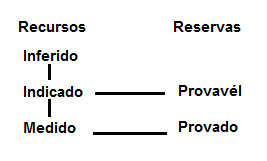
\includegraphics[scale=0.75]{./Capitulo_0/Recursos_Reservas.png}	
	\caption{Figura demonstrado a classificação de jazidas em recursos e reservas. Linhas indicando a transição entre as classificações }
	\label{Recursos_Reservas}
\end{figure}
\FloatBarrier


\subsection{Precisão e Exatidão}


Uma das premissas utilizadas na geoestatística clássica é que os resultados das amostras obtidas é um valor fixo. Esta afirmação na maioria dos casos não é realista, pois as amostragens na mineração podem apresentar diferentes valores referentes aos erros de amostragem. 

\begin{proposition}
	\textit{Para os processos de geoestatística clássica, os valores das amostras georeferenciados são determinísticos, a medida que apresentam volume, posicionamento e propriedades constantes. Isto não se aplica a todos os métodos geoestatísticos como o KVME (Kriging with Measurement Error Variance) \cite{delhomme1978applications}}
\end{proposition}


Esta variação das amostras quanto ao valor esperado por elas pode ser definido por duas propriedades: \textbf{Exatidão} e \textbf{Precisão}.  A Exatidão pode ser exemplificado como a proximidade de uma estimativa com a realidade, enquanto precisão é a medida da dispersão entorno de uma estimativa. Analogamente a precisão e a exatidão podem ser comparadas com um jogo de dardos como na figura \eqref{exat_prec}, em que pretendemos atingir o centro do alvo. Quanto mais próximo forem os disparos do centro, melhor será a sua exatidão, e quanto mais próximos forem os disparos entre si, significa que são mais precisos. Disparos podem ser precisos, no entanto, não exatos. Disparos podem ser exatos por se localizarem em média próximos do centro, mas podem ser imprecisos se distanciarem entre si. 

\FloatBarrier
\begin{figure}[!htb]
	\centering
	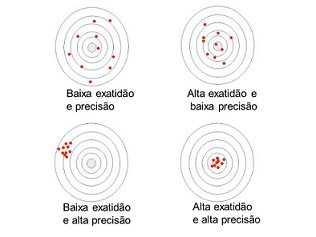
\includegraphics[scale=1.4]{./Capitulo_0/exat_prec.jpg}	
	\caption{Figura demonstrando os conceitos de exatidão e precisão. O centro do alvo é o valor verdadeiro que pretende-se alcançar com os disparos. Disparos entorno do centro são considerados exatos. Disparos próximos aos outros são considerados precisos }
	\label{exat_prec}
\end{figure}
\FloatBarrier

A amostragem na mineração ainda sofre um outro problema, quanto a reprodutibilidade, Na verdade este é um problema para a maioria dos fenômenos espaciais, pois quando amostramos uma região não há como amostrar novamente, pois estas amostras geralmente são \textbf{destrutivas}. Além disso, ao amostrar em um local específico, uma amostra mesmo que próxima já se configura como uma amostra diferente. Os trabalhos do professor \citet{gy2012sampling} invocam os principais conceitos e teorias a respeito da amostragem a granel, utilizada na mineração.

Eventualmente diversos fatores podem causar as variações e erros na amostragem. Há vários tipos de erros potenciais na estimativa de reservas minerais incluindo:

\begin{itemize}
	\item Erro de amostragem 
	\item Erros de análise química.
	\item Erros de densidade (É comum em muitos casos considerar a densidade do material constante ao longo do depósito)
	\item Erros da geologia, durante as fases de determinação da continuidade espacial e geometria do depósito mineral.
	\item Na escolha do método de lavra adotado que pode não atender as questões de seletividade do minério e estéril de forma ótima.
	\item A diluição do minério com a encaixante.
	\item Erro humano (inserção de valores errados no banco de dados, de casas decimais, et.)
	\item Fraude ( salgamento de amostras, substituições de amostras, dados não representativos, etc.)
	
\end{itemize}


\section{Conclusões} 

Neste capítulo inicial apresentamos os principais conceitos relacionados à geoestatística e ao planejamento de mina. Definimos o que é esta ciência que será abordada ao longo de todo o livro, o que ela pode realizar ou não, e sua importância dentro do contexto da mineração. Entendemos que a geoestatística é uma ferramenta para auxiliar na compreensão do desconhecido, e que é inerente ao empreendimento mineral, pois raras são as alternativas ao qual possuímos informação sistemática ao longo de todo o depósito mineral.


\section{Exercícios}
\begin{exercise} 
	Segundo a definição de \citet{carrasco2008additivity}, sabemos que uma variável é aditiva se o seu valor médio é igual a média de seus valores. Discutimos ao longo do texto que as variáveis teor e conteúdo metálico são variáveis aditivas, capazes de serem utilizadas nos modelos clássicos que abordamos neste livro. Desta forma identifique variáveis na mineração que podem ser consideradas aditivas ou não.

\end{exercise}
\begin{exercise}
	Realize um "brainstorm" e pense todas as possibilidades que podem sofrer uma mina que possam tornar um minério em um estéril. Por exemplo, a descoberta de uma outra jazida de uma empresa concorrente mais próximo do mercado consumidor pode aumentar o preço do minério e tornar parte do recurso inutilizável por um tempo. E quais seriam os fatores que fazem um estéril se tornar minério? 
\end{exercise}
\begin{exercise}
	Pretende-se determinar se uma unidade seletiva de lavra é um minério ou estéril. O custo fixo de extração do material é 5 um/ton. O custo de mineração por tonelada movimentada é 2 um/ton. A relação estéril/minério é 3/2. A Recuperação metalúrgica é de 95\% e o preço do minério é de 100 um/ton. O teor do elemento útil do bloco é 2\%. 
\end{exercise}

\begin{exercise}

Os dados da tabela seguinte demonstram um conjunto de valores estimados e dados reais obtidos. Determine:

a) O viés das estimativas. (Diferença entre a média dos valores estimados e a dos reais)

b) Considere o cut-off como 2g/ton. Determine: A proporção dos valores estimados como minério que realmente são minério. A proporção dos valores estimados como estéreis que realmente são estéreis. 

	\begin{tabular}{lllll}
		\hline
		Estimados & Real &  &  &  \\ \hline
		2.05      & 2.0  &  &  &  \\
		2.03      & 2.02 &  &  &  \\
		1.01      & 1.32 &  &  &  \\
		2.31      & 3.45 &  &  &  \\
		3.02      & 1.02 &  &  &  \\
		2.76      & 2.19 &  &  &  \\
		3.08      & 4.01 &  &  &  \\
		3.74      & 3.67 &  &  &  \\
		1.02      & 1.43 &  &  &  \\
		1.00      & 1.01 &  &  &  \\
		2.03      & 1.05 &  &  &  \\ \hline
	\end{tabular}
\end{exercise}






\chapter{Variáveis aleatórias regionalizadas} \label{cap_var_reg}

\begin{myquoting}{Kato Lomb}
	
	Todas as vezes que eu leio relatórios estatísticos, eu tento imaginar meu contemporâneo infortunado, a Pessoa Média, a quem, de acordo com estes relatórios, possui 0.66 filhos, 0.032 carros e 0.046 TVs. 
	
\end{myquoting}

\section{Introdução ao capítulo}

A geoestatística é uma ciência que se inicou nos anos de 1950, com estudos de \citet{krige1960departure}  na África do Sul a respeito de valores estimados em distribuições lognormais de ouro. Em 2012 o professor Daniel Krige recebeu a Ordem de Baobab, uma condecoração do presidente da África do Sul, pelas suas excepcionais contribuições para a economia, ciência, medicina, inovações tecnológicas e serviços comunitários. Durante seus 30 anos de idade,  se tornou pioneiro no uso da estatística para avaliação de depósitos de ouro para um número limitado de furos de sondagem. As ideias do pesquisador foram fortemente abraçadas pela França após a tradução de seus artigos em língua nativa em 1995, o que gerou a fundação do centro de Geoestatística em Fontainebleau, corroborando para os estudos do professor George Matheron, e a criação da \textbf{teoria das variáveis regionalizadas}.


 Este primeiro capítulo introduz a geoestatística a partir do seu objeto de estudo, as variáveis regionalizadas. Explicamos os principais conceitos abordados pela teoria clássica, e como eles se relacionam no entendimento dos fenômenos espacializados. Maiores informações podem ser encontradas nas obras de Matheron \cite{matheron1963principles} ou nos livros base de \cite{isaaks1989applied} e \cite{goovaerts1997geostatistics}


\section{Variáveis aleatórias} 

Alguns conceitos iniciais sobre estatística são necessários antes que possamos aprofundar os conceitos de geoestatística. Um dos principais conceitos utilizados para o entendimento de fenômenos aleatórios é o de \textbf{variável aleatória}. 

\begin{definition}[Variável aleatória] 
	\textit{Uma variável aleatória é uma função de um espaço amostral S nos números reais.} \citet{casella2010inferencia}
\end{definition} 

Imagine que tenhamos um saco com grandes quantidades de pedras coloridas vermelhas e azuis. Nosso espaço amostral seria portanto \textbf{S=\{pedras vermelhas, pedras azuis\}}. Se quisermos determinar uma variável aleatória que seja definida pela amostragem de duas pedras poderíamos ter o seguinte resultado \textbf{Z =\{(pedra vermelha, pedra azul) , (pedra vermelha, pedra vermelha), (pedra azul, pedra azul)\}}. Uma variável aleatória geralmente é definida a partir de uma letra maiúscula, enquanto uma realização, ou seja, um resultado desta variável aleatória é definido por uma letra minúscula. A figura \ref{Indicadora} é um exemplo de uma variável aleatória, pois para cada valor possível dentro do espaço amostral de diferentes litologias é associado um valor inteiro. 

\FloatBarrier
\begin{figure}[!htb]
	\centering
	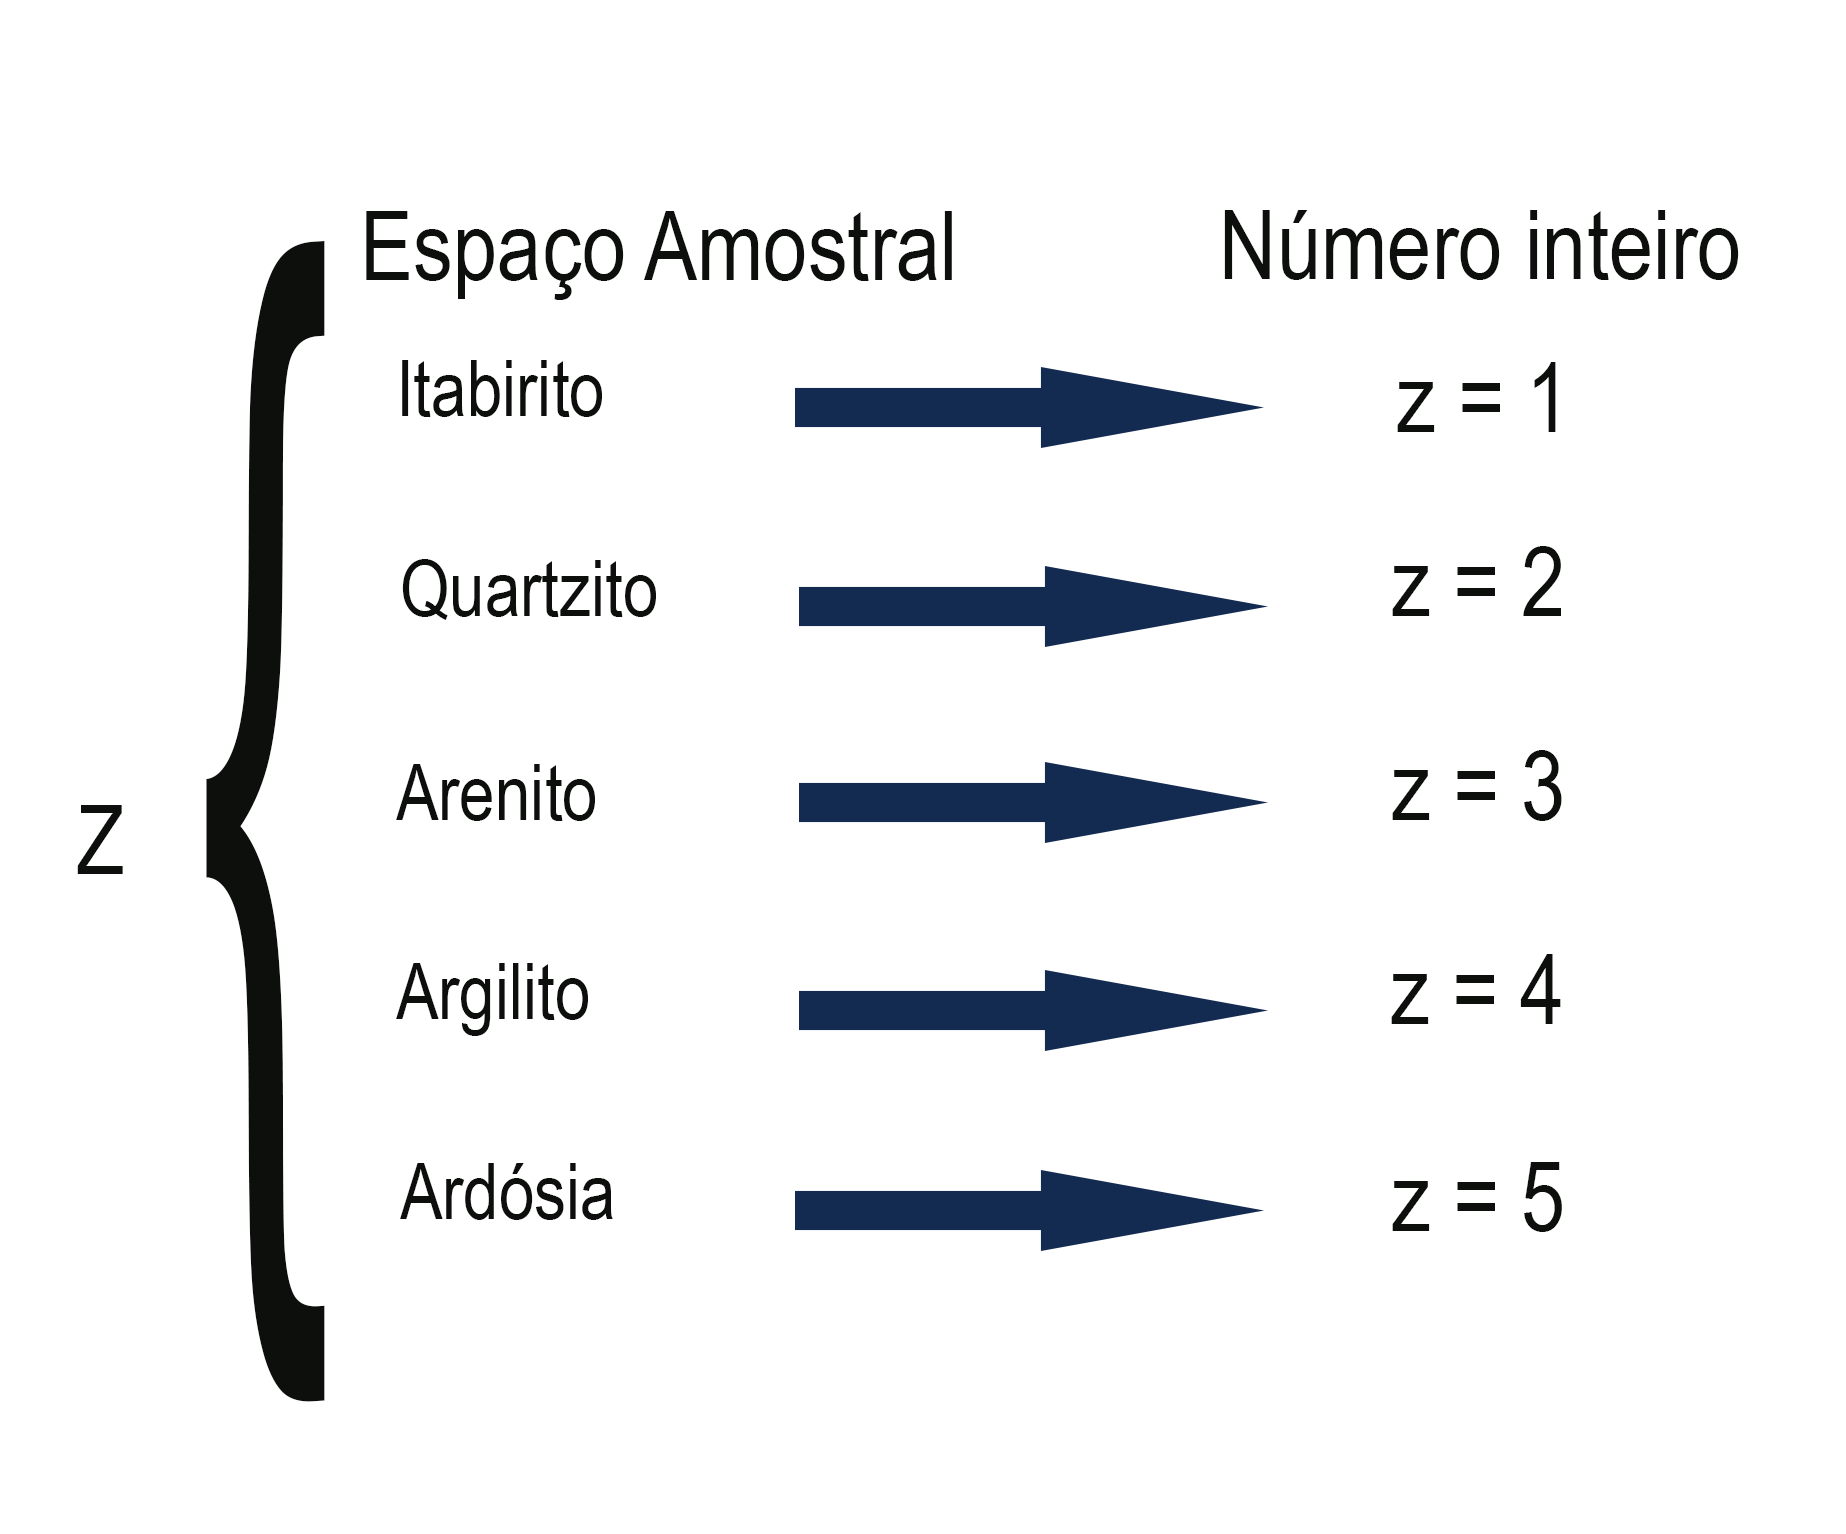
\includegraphics[scale=0.7]{./Capitulo_1/Indicadora.png}	
	\caption{Exemplo de variável aleatória indicadora. Para cada possível valor de litologia do depósito é associado um valor inteiro. }
	\label{Indicadora}
\end{figure}
\FloatBarrier

Note, no entanto, que atribuir um valor para esta variável não significa dar uma maior importância ou uma menor importância para cada litotipo. Colocar um valor inteiro igual a 1 para o Itabirito não significa considerá-lo mais importante que as demais litologias. Neste caso dizemos que esta variável é \textbf{cardinal}, pois o valor associado de cada componente do espaço amostral a um valor inteiro não está diretamente ligado com sua importância, ao contrário de variáveis \textbf{ordinais} ao qual seu número associado é diretamente expresso pela sua importância.

 As variáveis aleatórias são divididas geralmente em duas classes na geoestatística, considerando \textbf{variáveis aleatórias reais}, que podem apresentar valores dentro do conjunto de dados reais, ou \textbf{variáveis indicadoras}, quando consideramos que podem assumir valores inteiros. Exemplos de variáveis reais, por exemplo, são as de teores dos elementos metálicos, enquanto variáveis indicadoras são representadas pelas litologias presentes no depósito mineral. 
 
 Variáveis ditas \textbf{contínuas} são aquelas que possuem um espaço amostral infinito e  \textbf{não contável},  geralmente representada por um conjunto de valores reais. Quando medimos teores, por exemplo, o resultado de uma amostra pode variar infinitamente dentro de um intervalo de 0\% a 100\%. Apesar desta limitação, o número de realizações que podem advir desta variação são infintas, pois naturalmente o valor 5,6740 \% é diferente do valor 5,6741 \%, mesmo que muito próximos.
 
 Em contrapartida, variáveis discretas são \textbf{contáveis}, mesmo que seu espaço amostral seja infinito. Se um subconjunto deste espaço amostral for considerado é possível conseguir definir para ele uma probabilidade. Variáveis discretas estão geralmente ligadas ao conjunto de números inteiros.
 
  Para uma variável aleatória pode ser atribuído uma probabilidade $(Pr)$ de ocorrência para cada uma de suas realizações. A ideia de probabilidade mais básica está relacionada com a \textbf{frequência de ocorrência relativa de um evento}, ou também chamada de abordagem frequentista. Nossa variável aleatória demonstrada pela figura \ref{Indicadora} pode ser associada a uma probabilidade de acordo com a figura \ref{Prob}, considerando a proporção de rochas de cada tipo dentro do domínio geológico estimado. 
  
  \FloatBarrier
  \begin{figure}[!htb]
  	\centering
  	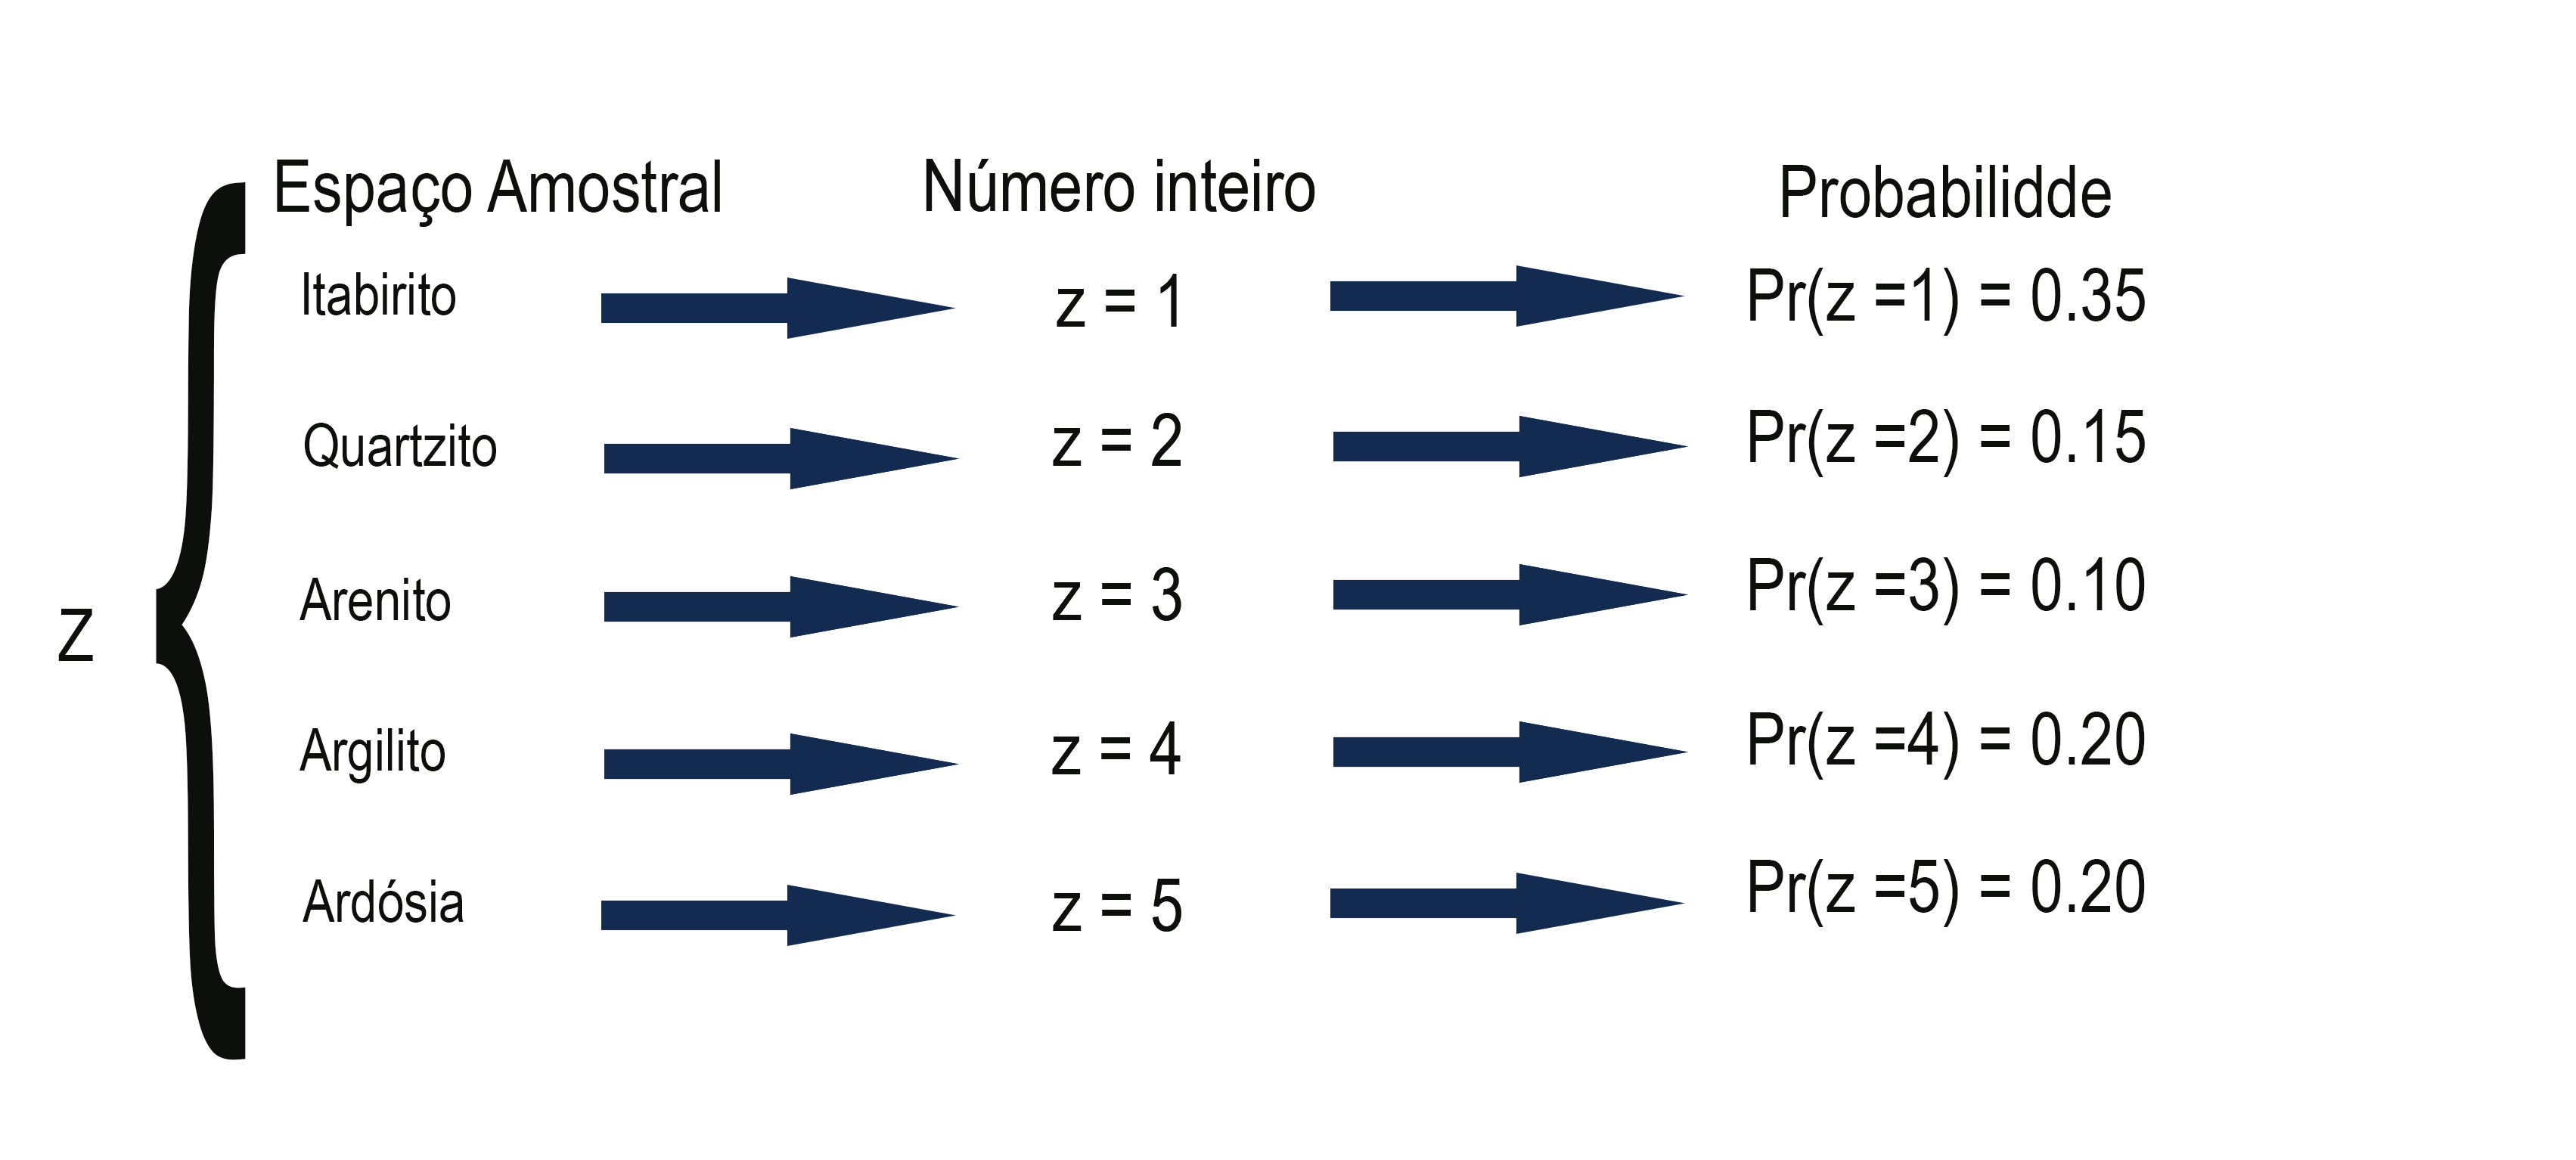
\includegraphics[scale=0.7]{./Capitulo_1/Prob.png}	
  	\caption{Exemplo de variável aleatória indicadora. Para cada possível valor de litologia do depósito é associado um valor inteiro. Uma probabilidade é atribuída para a frequência relativa de cada litologia. }
  	\label{Prob}
  \end{figure}
  \FloatBarrier
  
  Em outras palavras a probabilidade é semelhante a uma métrica de proporção das realizações de uma variável aleatória. Na verdade a probabilidade pode ser qualquer medida, desde que satisfaça os \textbf{Axiomas de Kolmogorov}. 
  
  \begin{enumerate}
  	\item A probabilidade de um evento é um número não negativo, dentro do intervalo [0,1].
  	\item A probabilidade do espaço amostral é 1.
  	\item Se n eventos são mutuamente exclusivos, a probabilidade da união destes eventos é igual a soma das probabilidades individuais.
  \end{enumerate}
  
    Os conceitos de probabilidade são estudados na matemática dentro da \textbf{teoria dos conjuntos}  que é a base para a fundamentação da estatística. Para maiores informações da teoria base em probabilidade, axiomas de Kolmogorov e teoria dos conjuntos, aconselhamos ler as referências de \citet{alencar2014teoria} e \citet{feitosa2011teoria}.
 
 \section{Função de distribuição acumulada - fda}  
 
Para cada elemento de uma variável indicadora podemos associar um valor de probabilidade, ou de frequência da apresentação deste elemento. Por exemplo se consideramos que um depósito mineral possui apenas dois tipos de rocha, podemos dizer que o tipo 1 representa 30\% de frequência no depósito mineral, enquanto o tipo 2 apresenta 70\% de frequência. Associar uma probabilidade para variáveis aleatórias indicadoras é intuitivo. No entanto, não conseguimos definir a probabilidade de um elemento para variáveis aleatórias reais contínuas, pois o espaço amostral é infinito. Não conseguimos associar, por exemplo, a probabilidade de um teor ser 5,67\%. Neste caso utilizamos uma abordagem intervalar, associando a probabilidade a um intervalo de valores reais, logo é possível dizer que o depósito mineral possui probabilidade de 40\% dos teores variarem de 5,67\% a 9,32\%. Uma função de distribuição acumulada é representada pela probabilidade de uma variável aleatória assumir um valor igual ou menor a um determinado limite. Definimos então a \textbf{Função de distribuição acumulada $F(z)$} tal como  

\begin{equation}
F(z) = \Pr(Z \leqslant z)
\end{equation}

A figura \ref{distribuicoes} indica a função de distribuição para variáveis contínuas e discretas. Em A) possuímos uma função discreta que pode assumir apenas valores inteiros de 1 a 8. Em B) possuímos uma função contínua de valores que se alteram no intervalo [1,8]
	
	
\FloatBarrier
\begin{figure}[!htb]
	\centering
	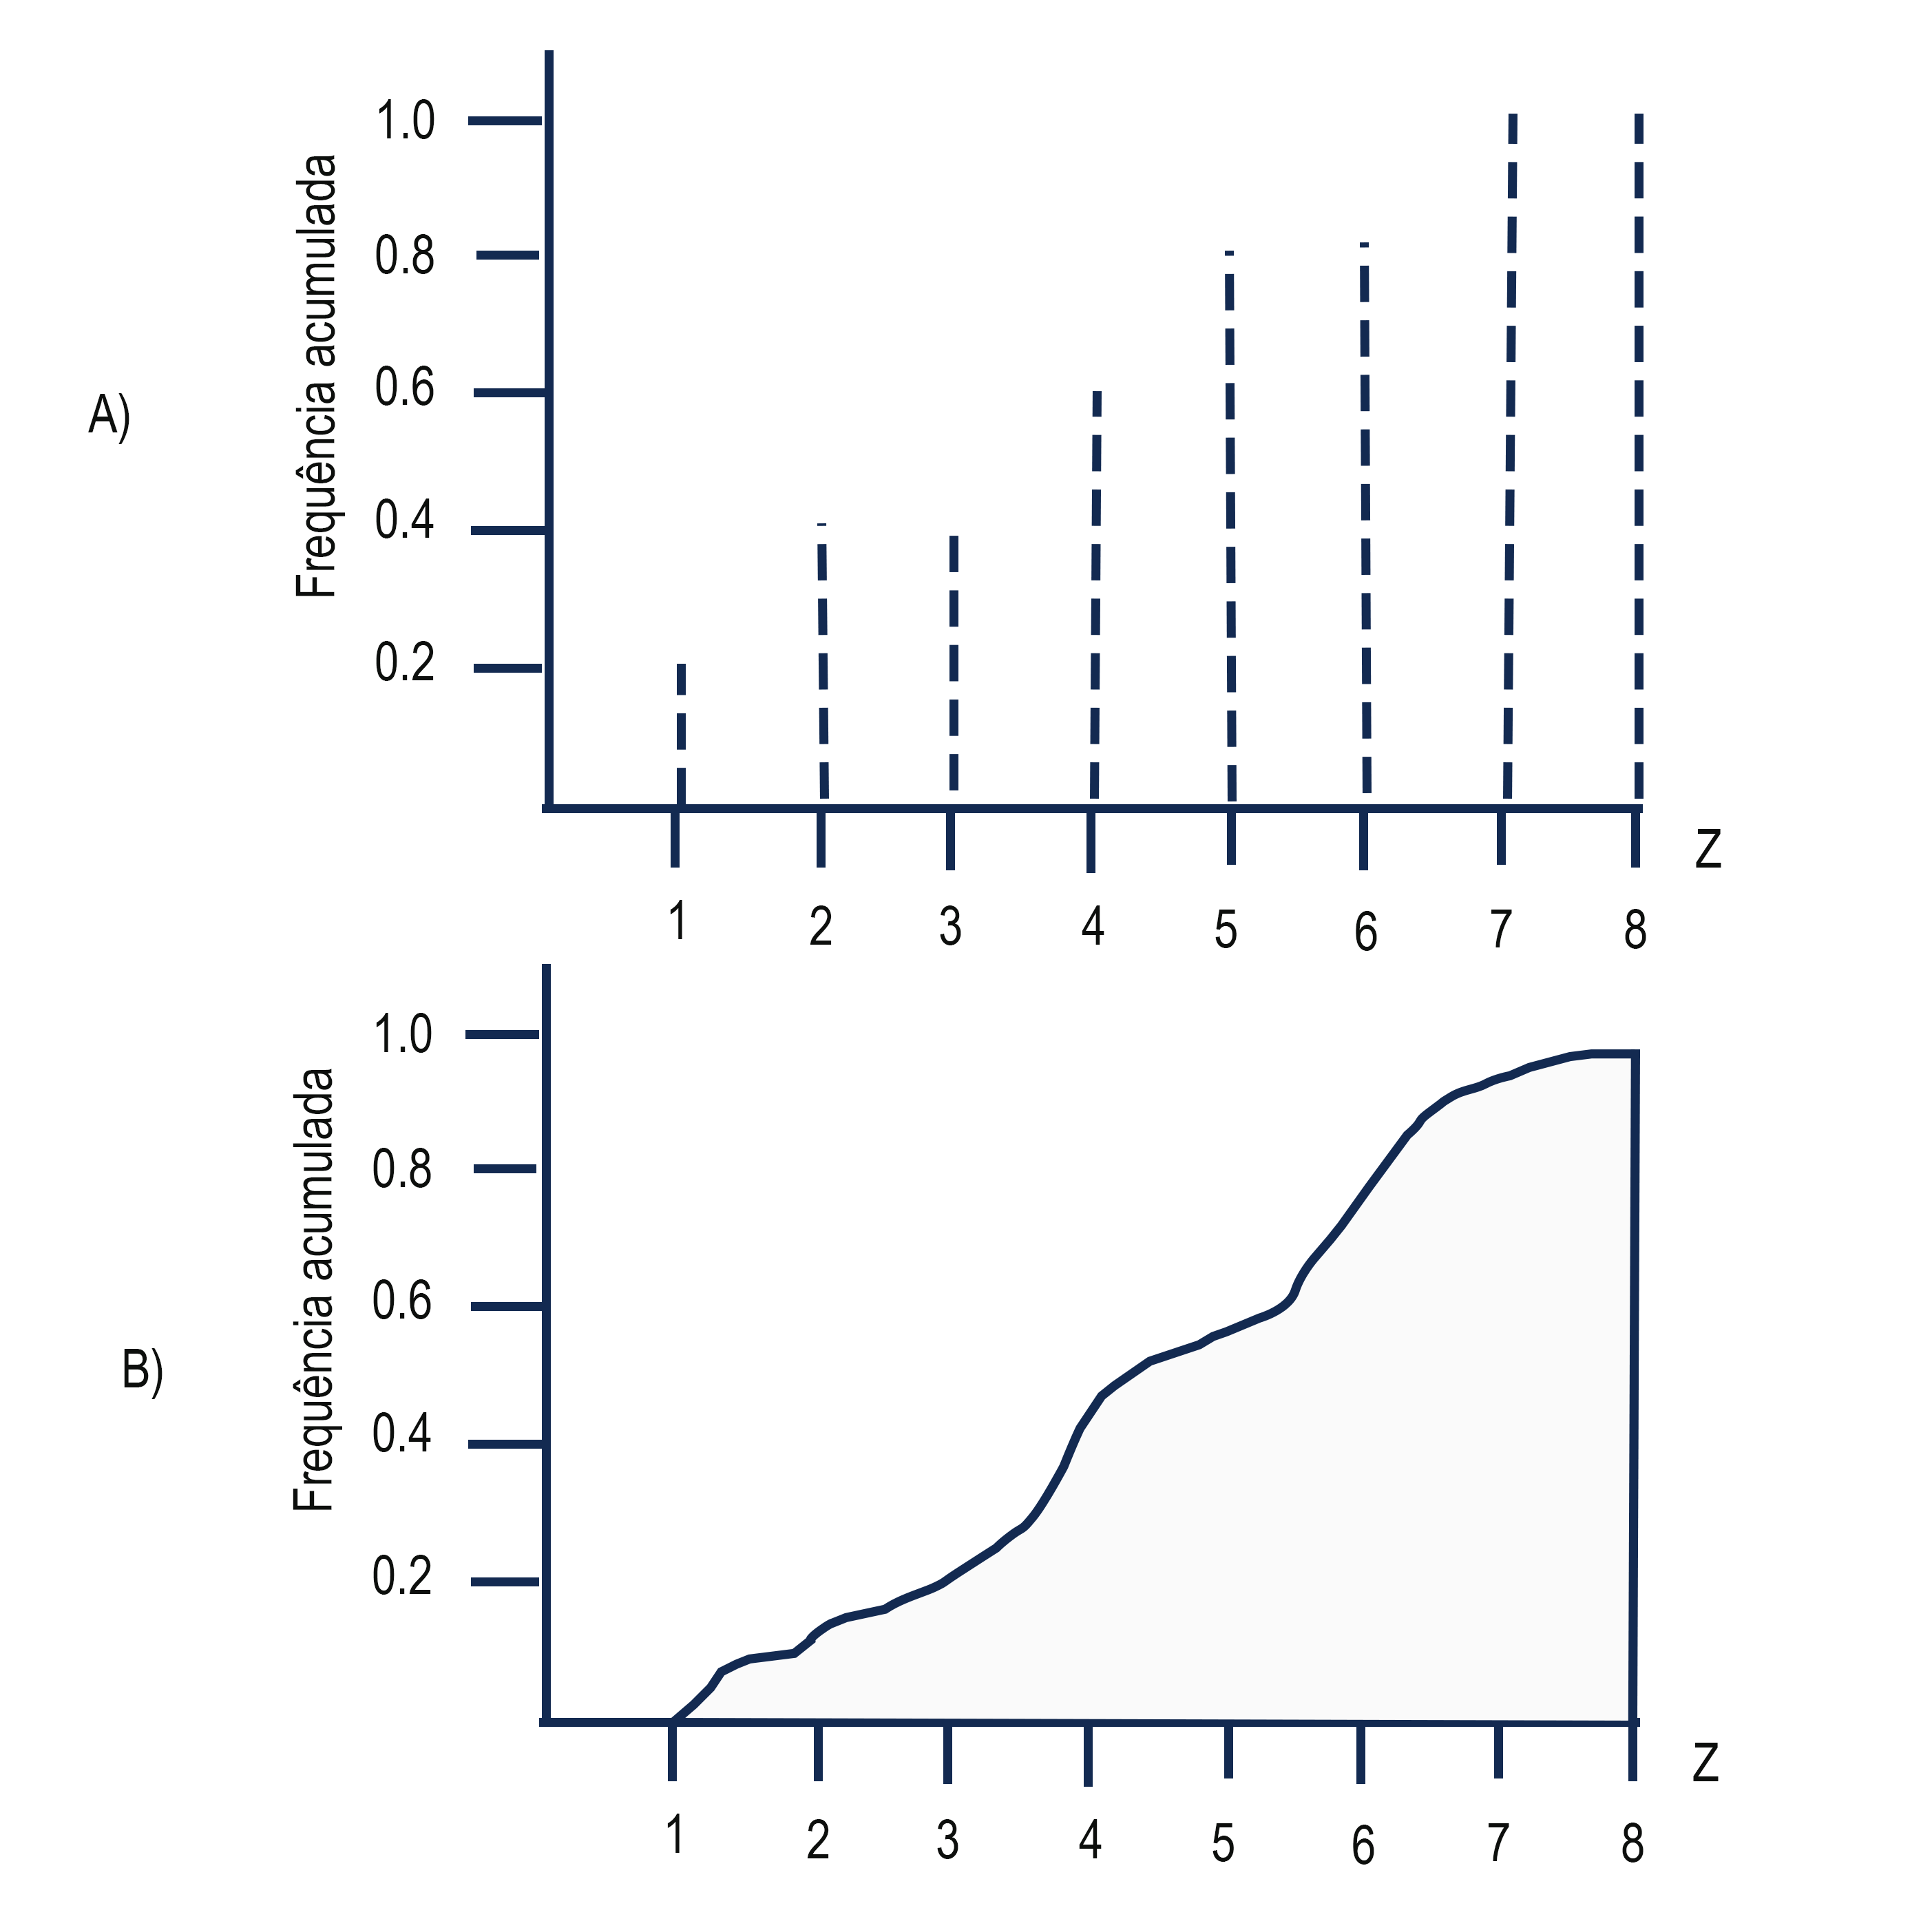
\includegraphics[scale=0.5]{./Capitulo_1/Distribuicoes.png}	
	\caption{Função de distribuição acumulada - fda para variáveis discretas A) e contínuas B) }
	\label{distribuicoes}
\end{figure}
\FloatBarrier

\section{Função de densidade de probabilidade - fdp}  

No caso de distribuições contínuas, em que os valores podem ser determinados para qualquer valor dentro de um domínio real, é permitido utilizar princípios de cálculo para medir informações dessas distribuições. Como não podemos definir o valor da probabilidade em um ponto específico precisamos utilizar o conceito de probabilidade intervalar. A \textbf{Função de densidade de probabilidade-fdp} pode ser determinada como a probabilidade um valor assumir este valor dada uma variação infinitesimal.

\begin{equation}
f(z) = lim_{\delta \rightarrow 0}\left [ Pr(Z > z, Z < z + \delta ) \right ]
\end{equation}

Logo a relação entre a função de distribuição acumulada e a função de densidade de probabilidades pode ser expressa por 

\begin{equation}
F(z) = \int_{-\infty }^{z} f(z) dz
\end{equation}

\begin{proposition}
	\textit{Pode parecer que o valor da densidade de probabilidade seja equivalente ao valor da probabilidade assumindo uma realização $z$ de variável aleatória $Z$, no entanto esta visão está errada! A ideia de probabilidade está diretamente ligada na ideia de frequência relativa de um evento. Valores de variáveis contínuas possuem espaço amostral incontável, o que significa que não conseguimos medir o seu tamanho, sendo ele infinito. Quantos seriam os possíveis resultados, por exemplo, de um teor de uma amostra apresentar? Se fosse possível associar uma probabilidade a um valor de uma variável aleatória real, todos estes valores seriam iguais a zero, pois sua frequência em nada representa na imensidão de valores possíveis. A função de densidade de probabilidade é na verdade uma medida de taxas de variação da probabilidade.}
\end{proposition}

\section{Variáveis regionalizadas} 

\citet{matheron1963principles} , pai fundador da geoestatística, iniciou o conceito de \textbf{variável regionalizada}, para exemplificar os fenômenos espaciais. Quando um fenônmeno exibe uma certa \textbf{estruturação espacial}, dizemos ele ser regionalizado. Os fenômenos geológicos, por exemplo, exibem estruturação característica na sua formação, o que significa que os corpos geológicos apresentam geometrias características de suas gêneses. A variável regionalizada $z(x)$ denota um valor conhecido em um determinado ponto $x$, sendo apenas um resultado neutro puramente descritivo, sem interpretação probabilística. Em outras palavras, a variável regionalizada é o valor real encontrado no depósito mineral para cada ponto $x$ no espaço. 

\begin{definition}[Variável Regionalizada]
	\textit{Uma variável regionalizada $z(x)$ representa a medida de uma propriedade qualquer, seja ela o teor do elemento metálico, quantidade de metal ou acumulação, definida em um ponto $x$ no espaço de coordenadas definidas}
\end{definition}

É impossível para nós conhecer o valor real de $z(x)$ para cada ponto no espaço, pois implicaria em muito mais que uma amostragem sistemática por todo o domínio do depósito mineral. Desta forma a variável regionalizada apresenta aspectos contraditórios, porém complementares para a definição do modelo geoestatístico:

\begin{itemize}
	\item \textbf{Apresenta uma componente aleatória} onde não conseguimos amostrar ou definir a variável. Isto marca o aspecto irregular da variável. Seguindo a notação estatística, nos locais onde a variável regionalizada não é definida, denotamos $Z(x)$ para informar que nestes locais ela assume aspecto de uma variável aleatória. Sendo $\Omega$ o universo que pode ser composto a variável, definimos a variável aleatória em local desconhecido da variável regionalizada como $Z(x):\Omega \rightarrow \Re $.
	\item \textbf{Apresenta uma componente estruturada} nos locais onde é determinada, como por exemplo, pelos métodos de amostragem, representada pela própria forma $z(x)$, convencionalmente pela notação estatística como a realização da variável aleatória $Z(x)$ no suporte $x$. 
\end{itemize}

\begin{proposition}
	\textit{Pode parecer um tanto estranho que algo possa assumir condições dicotômicas desta forma. Ao mesmo tempo que consideramos que algo existe e é determinístico, também consideramos que algo é aleatório e transitório. Na verdade as coisas são como sempre são, o que fazemos é assumir que em certos casos, não conseguimos definir algo, e em outro sabemos muito bem o que é. A aleatoriedade, na verdade, nunca existiu. Aleatoriedade é nosso princípio de humildade em não entendermos como os fenômenos ocorrem.}
\end{proposition}

A observação da variável regionalizada, não ocorre, no entanto em um ponto do espaço. Pontos são abstrações matemáticas de dimensão infinitesimal, uma condição geralmente para que possamos aplicar o princípio de continuidade dos modelos. As nossas observações são realizadas em amostras com volumes específicos e em grandes regiões que queremos estimar. \citet{matheron1963principles} apresenta os principais conceitos de domínio e suporte. Um domínio é uma região onde a variável regionalizada é diferente de zero. No nosso livro apresentamos o domínio das estimativas pela notação $D$, enquanto os domínios de um bloco ou painel de lavra são apresentados por $V$.


\begin{definition}[Domínio]
	\textit{Domínio de uma variável regionalizada pode ser considerada qualquer região onde a variável apresenta valor diferente de zero. Por exemplo, a região da mina onde pretendemos estimar valores desconhecidos pode ser considerada como um domínio de estimativa D.}
\end{definition}

\citet{matheron1963principles} apresenta também o conceito de suporte,  sendo este relacionado com a capacidade de entendimento da variável regionalizada $z(x)$. De certa forma, é impossível conhecer o valor da variável regionalizada em um ponto $x$, pois o que detemos é o conhecimento da variável em um volume $v$, representando um testemunho de rocha, ou um fragmento de rocha. 

\begin{definition}[Suporte]
	\textit{Suporte é o volume e forma $v$ ao qual se detém o conhecimento da variável regionalizada $z_{v}(X)$}
\end{definition}

Em alguns casos, pela dimensão do domínio estimado em relação ao suporte, este é quase observado como um ponto. Imagine um framento de rocha de $10cm^{3}$ e um painel a ser estimado de $200m^{3}$. A diferença de ordem de grandeza entre a amostra e o painel é gigantesca.

\begin{proposition}
	\textit{Dizemos que do ponto de vista matemático é quase impossível definir a variável regionalizada $z(x)$, pois é quase impossível amostrar em um ponto. No entanto, esta é uma observação muito purista, que desconsidera os aspectos de engenharia. Em alguns casos uma amostra pode ser visualizada como uma realização da variável regionalizada $z(x)$, pois o volume da amostra é tão inferior ao domínio, que se torna praticamente uma dimensão pontual}
\end{proposition}

Uma das condições de aplicação da geoestatística clássica, que considera o uso de variáveis aditivas, é que o suporte das amostras utilizado nas estimativas deve ser o mesmo. Isto significa que o volume dos testemunhos utilizados para estimativa, amostras de canais, ou outros tipos de amostragens devem ter todos mesma forma, tamanho e volume. Esta é também outra questão impraticável, pois é impossível principalmente em rochas, obter regularidade nas amostras desta forma. Para contornar esta situação nos utilizamos os métodos chamados de \textbf{regularização}, que permitem criar amostras de mesmo tamanho. 



Estas definições são as clássicas paresentadas pelo professor George Matheron em seus primeiros trabalhos sobre a teoria das variáveis aleatórias regionalizadas. Existe muita confusão entre diferentes autores para a representação destes conceitos de \textbf{suporte} e \textbf{domínio}, sendo muitas vezes o domínio do painel chamado de suporte do painel. De acordo com a definição de suporte, seria necessário conhecer o valor real do painel, o que é impossível, sendo mais adequada a nomeclatura de domínio do painel. Estas divergências de conceituação não prejudicam o estudo da geoestatística como um todo, mas acabam por criar diferentes formas de notação e algumas vezes dificultam a leitura dos textos. O mais importante em se ter em mente é que este volume, seja do domínio ou do suporte, pode alterar os resultados das suas estimativas, na chamada \textbf{relação volume e variância}.



Esta ambiguidade da variável regionalizada permite tratamento de forma diferenciada segundo os objetivos de cada estudo. Podemos, ora tratar a variável regionalizada apenas como valores dispostos no espaço, ora dar um tratamento probabilístico para estes valores. \citet{matheron1963principles} aborda estes dois princípios como 

\begin{itemize}
	\item \textbf{Métodos transitivos} Considera a hipótese de estacionaridade, mas não implica em qualquer hipótese probabilística, sendo métodos apenas descritivos da variável regionalizada $z(x)$. Esta abordagem é utilizada principalmente na geoestatística clássica abordada neste livro. Faremos os cálculos geoestatísticos considerando apenas a descrição dos valores amostrados em uma determinada região, sem premissas sobre uma possível distribuição de probabilidades local. 
	\item \textbf{Teoria intrínseca} Utiliza a intrepretação probabilística da variável regionalizada $Z(x)$, também considerando hipóteses de estacionaridade. Esta metodologia é amplamente utilizada nos métodos considerados não-lineares e nas simulações geoestatísticas, em que se pretende determinar não apenas um valor esperado determinístico para um volume estimado, mas também uma distribuição de probabilidades.  
\end{itemize}

\section{Funções aleatórias} 

Como dissemos anteriormente a variável regionalizada possui uma componente tanto determinística, onde conhecemos os valores da variável, como uma componente aleatória, em locais onde se desconhece a propriedade de interesse. Este aspecto dicotômico é trocado por alguns autores ao usarem da \textbf{teoria intrínseca} e estabelecerem a variável aleatória sobre termos exclusivos de uma interpretação probabilística.  Uma visão um pouco mais abstrata da variável aleatória é entender que sua componente determinística é apenas um resultado ou uma realização da variável aleatória naquele local, e que  $Z(x)$, chamada em alguns casos de \textbf{função aleatória} é uma função que associa a qualquer ponto do espaço uma variável aleatória.  A figura \ref{func_aleatoridade} demonstra o resultado de uma amostragem $z(x= x_{1})$ no ponto $x_{1}$.  


\FloatBarrier
\begin{figure}[!htb]
	\centering
	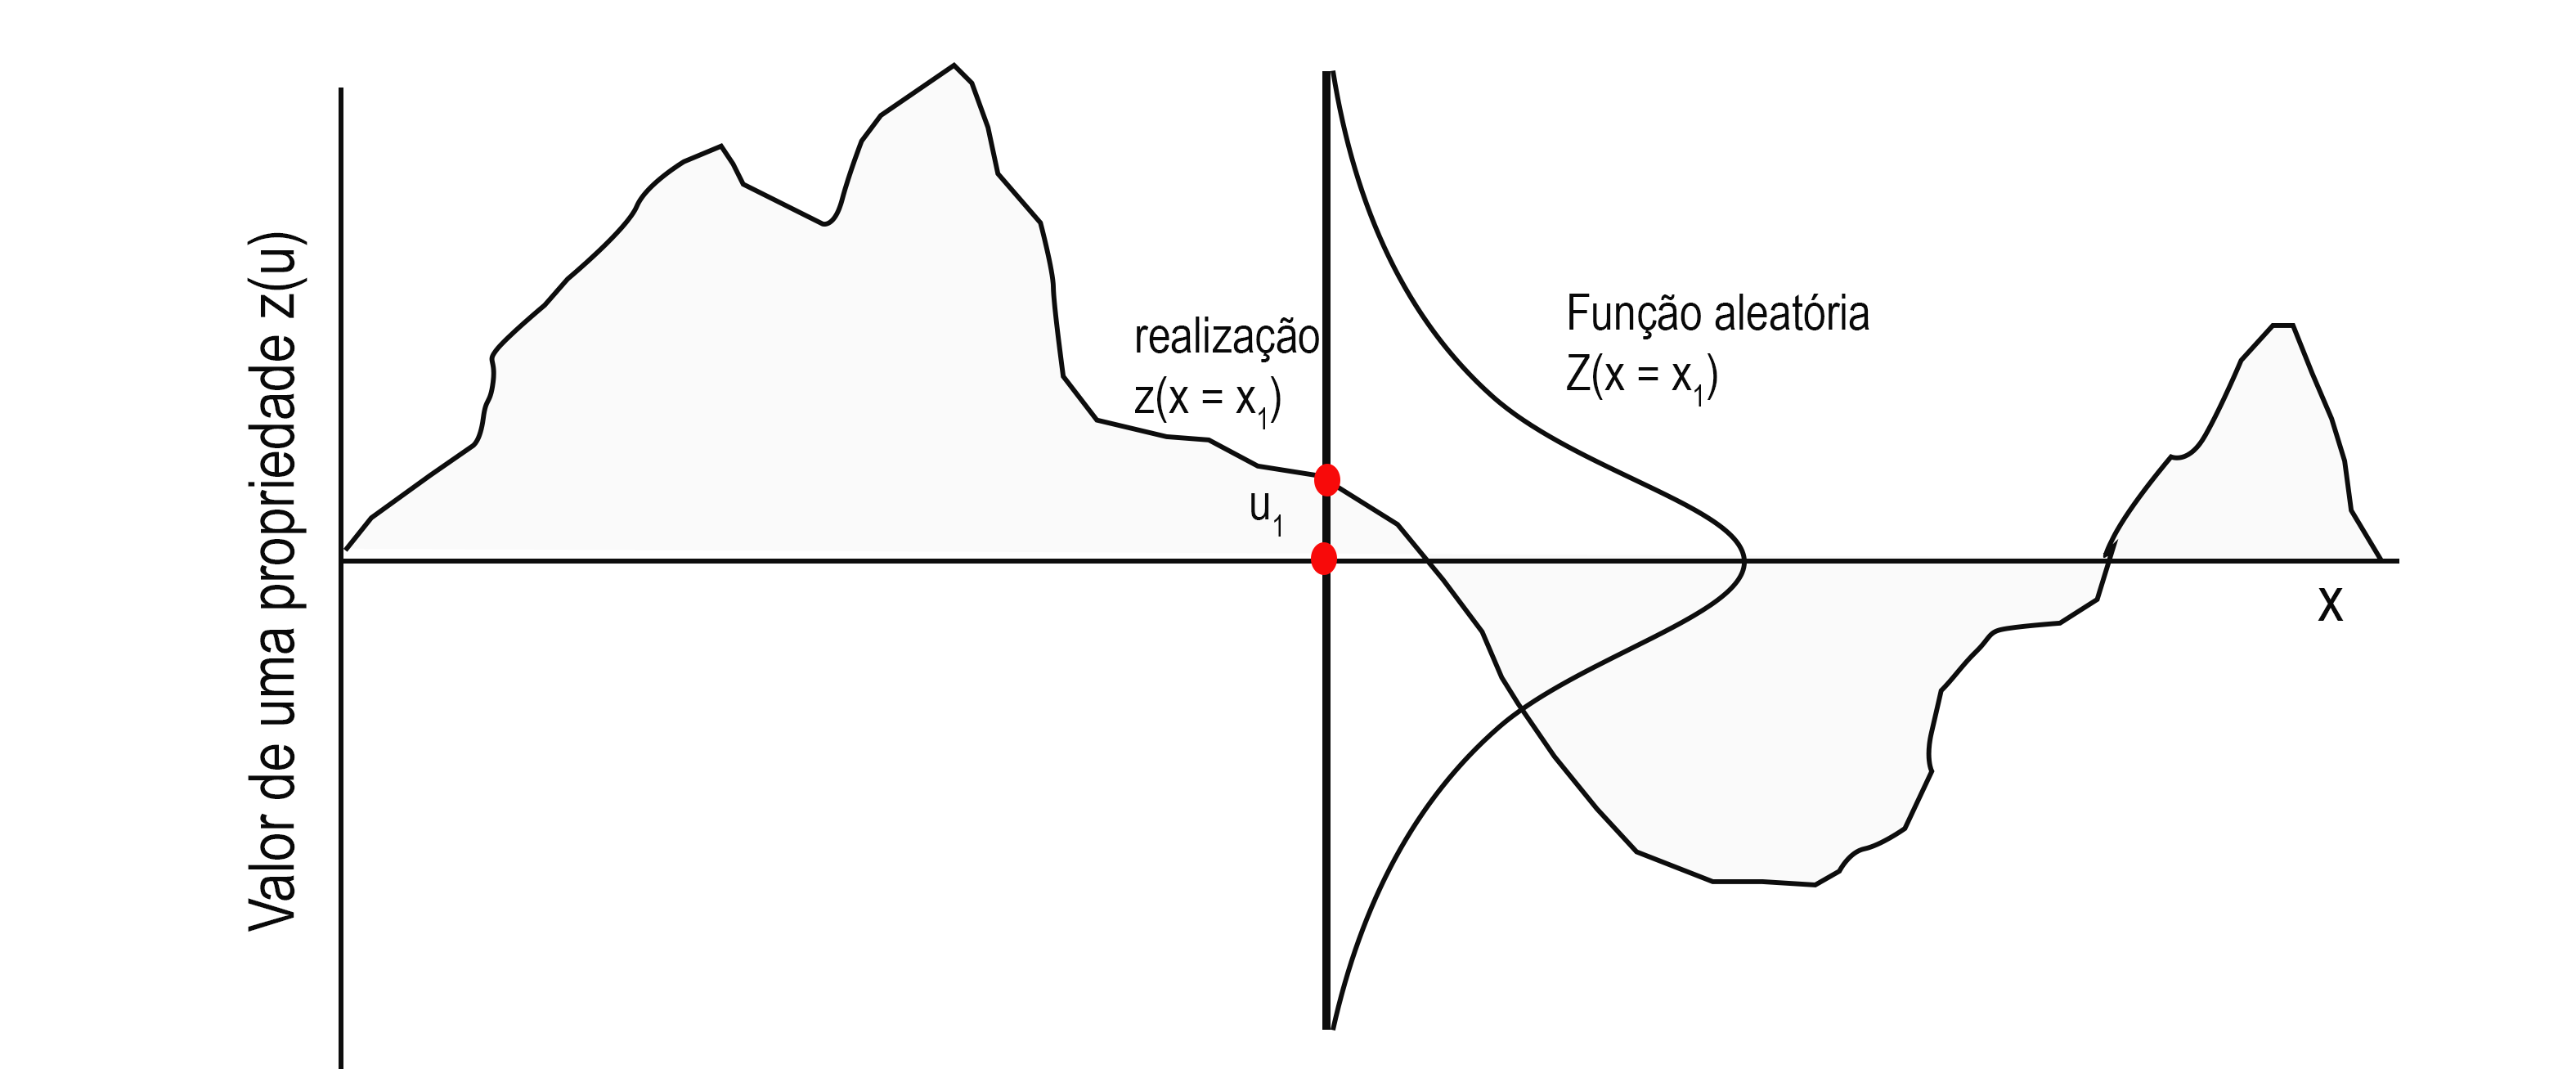
\includegraphics[scale=0.8]{./Capitulo_1/Variavel_aleator.png}	
	\caption{Demonstração do resultado amostrado $z(x = x_{1})$ como uma realização da função aleatória $Z(x = x_{1})$. No ponto $x_{1}$ o valor amostrado é apenas um resultado de uma função que desconhecemos, que associa uma distribuição de probabilidades naquele local. }
	\label{func_aleatoridade}
\end{figure}
\FloatBarrier

Em muitos os casos não é possível conhecer esta função geradora do depósito mineral, apenas tomamos como hipótese que ela existe e é uma combinação de variáveis aleatórias em todo o espaço. Na geoestatística muitas vezes consideramos que esta função pode ser representada como uma combinação linear destas variáveis, chamada de \textbf{geoestatística linear}, ou \textbf{geoestatística clássica}. Ao tomarmos esta simplificação proposta pela teoria intrínseca, a demonstração das técnicas geoestatísticas se tornam bem mais fáceis, por isso, durante este texto, pretendemos utilizar o conceito da função aleatória em vez da forma tradicional da variável regionalizada proposta por Matheron. 

\begin{definition}[Função aleatória]
	\textit{Uma função aleatória pode ser descrita como uma função que associa a cada ponto no espaço $x$ uma variável aleatória $Z(x =x_{1}))$, sendo $x_{1}$  o ponto de coordenas especificado. }
\end{definition}

Esta função aleatória é composta de uma amalgama de diversas variáveis aleatórias, cada uma em um ponto do espaço. A análise geoestatística destes valores permite decompormos esta função em duas componentes principais de acordo com os valores esperados de cada uma destas variáveis. O valor esperado tende a ser o de maior probabilidade de ocorrência em um determinado local. Desta forma podemos decompor a função aleatória em duas componentes principais, o \textbf{resíduo} e o valor de \textbf{tendência}. Por definição, a função aleatória pode ser expressa por $Z(x) = R(x) + m(x)$, sendo que os resíduos possuem média igual a zero.

\FloatBarrier
\begin{figure}[!htb]
	\centering
	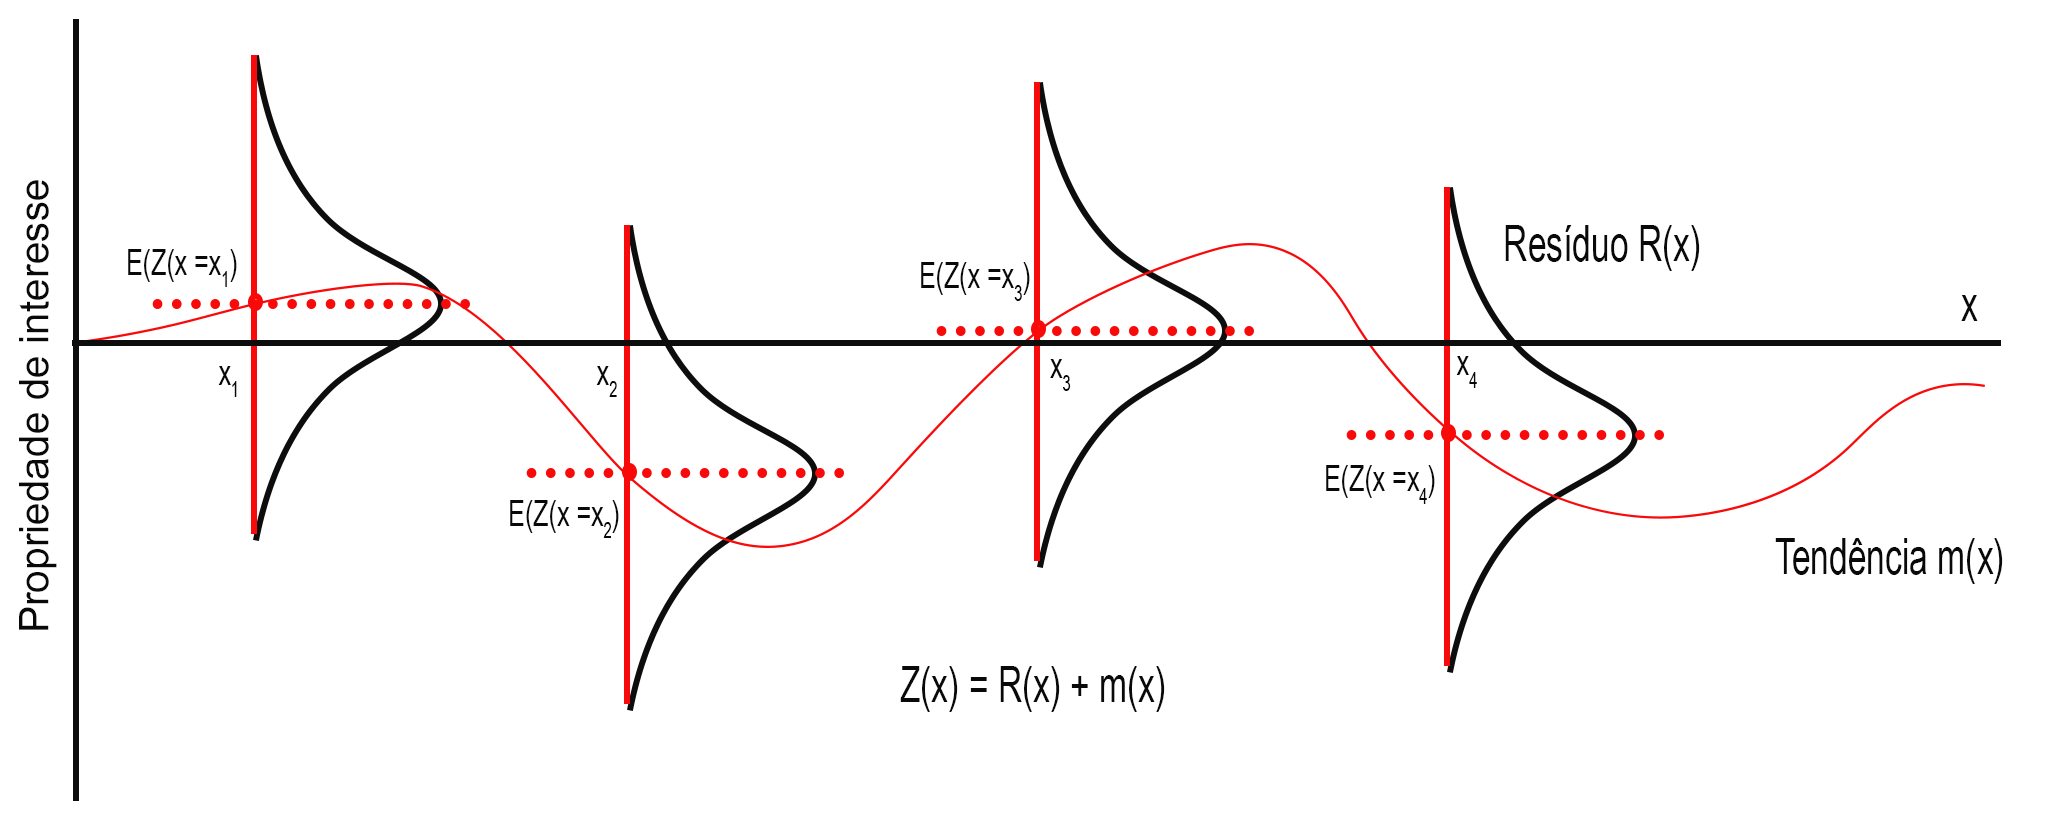
\includegraphics[scale=1]{./Capitulo_1/Decomp.png}	
	\caption{Decomposição da função aleatória a partir da determinação de sua tendência, indicada por $m(x)$, e o seu resíduo $R(x)$. }
	\label{decompos}
\end{figure}
\FloatBarrier


É comum na geoestatística assumirmos algumas hipóteses quanto a função aleatória. A \textbf{hipótese de estacionaridade de segunda ordem} afirma que o valor da tendência deve ser constante em todo o domínio considerado e o resíduo deve possuir variância constante para todo o domínio. Como desconhecemos a função aleatória, e nunca conseguimos determinar as variáveis aleatórias em cada ponto considerado, a hipótese de estacionaridade é sempre assumida, e nunca conseguimos comprová-la. Observe a série de números gerados na figura \ref{SerieA}. 

\FloatBarrier
\begin{figure}[!htb]
	\centering
	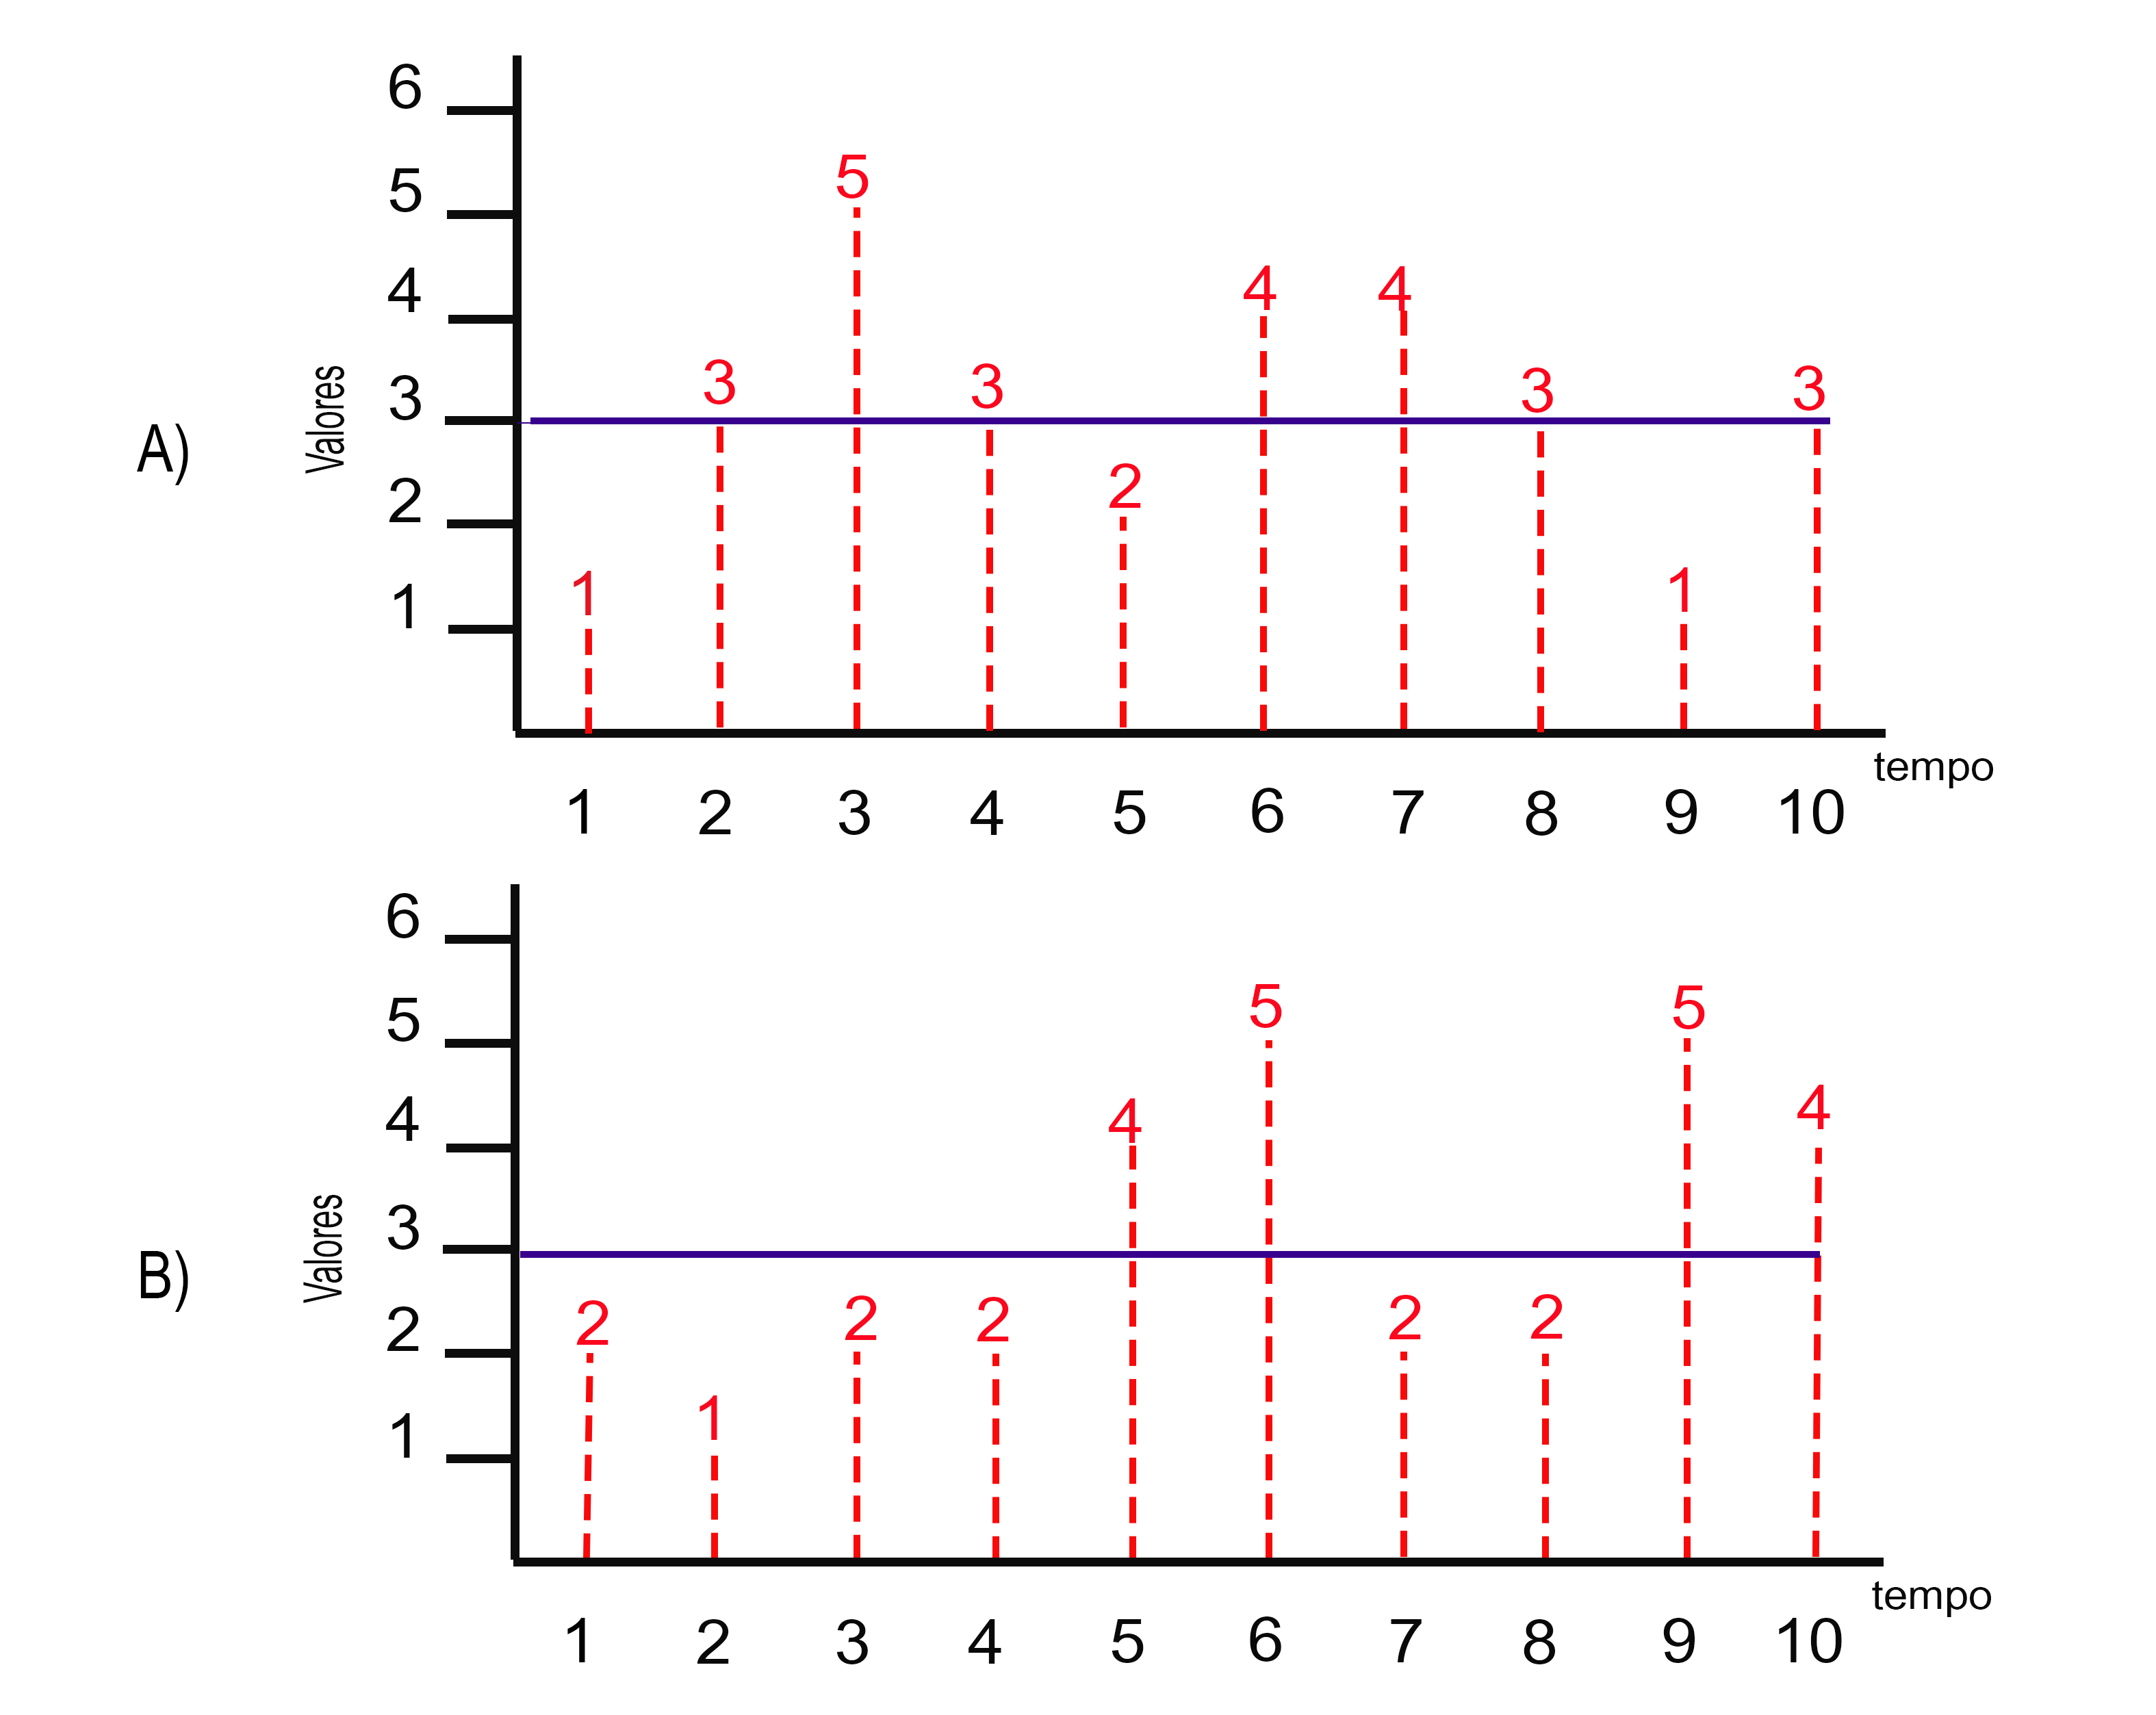
\includegraphics[scale=0.5]{./Capitulo_1/Serie_A.png}	
	\caption{Série de números gerados em A e B. O valor médio destas séries é 2.9.} 
	\label{SerieA}
\end{figure}
\FloatBarrier

Ao observá-los, provavelmente você deve estar imaginando que foram feitos jogando-se dados na mesa. As séries A e B possuem média muito próxima do que seria de um dado de seis lados, e variam de 1 a 6. Na verdade, você está parcialmente certo, eu gerei estes números a partir de dados. A diferença, no entanto, é que a série B foi gerada metade por um dado tetraédrico e metade por um dado cúbico, enquanto os dados da série A foram gerados apenas por um dado cúbico. Os valores médios reais que deveriam ser consideradas para este modelo são os representados na figura \ref{SerieB}. 


\FloatBarrier
\begin{figure}[!htb]
	\centering
	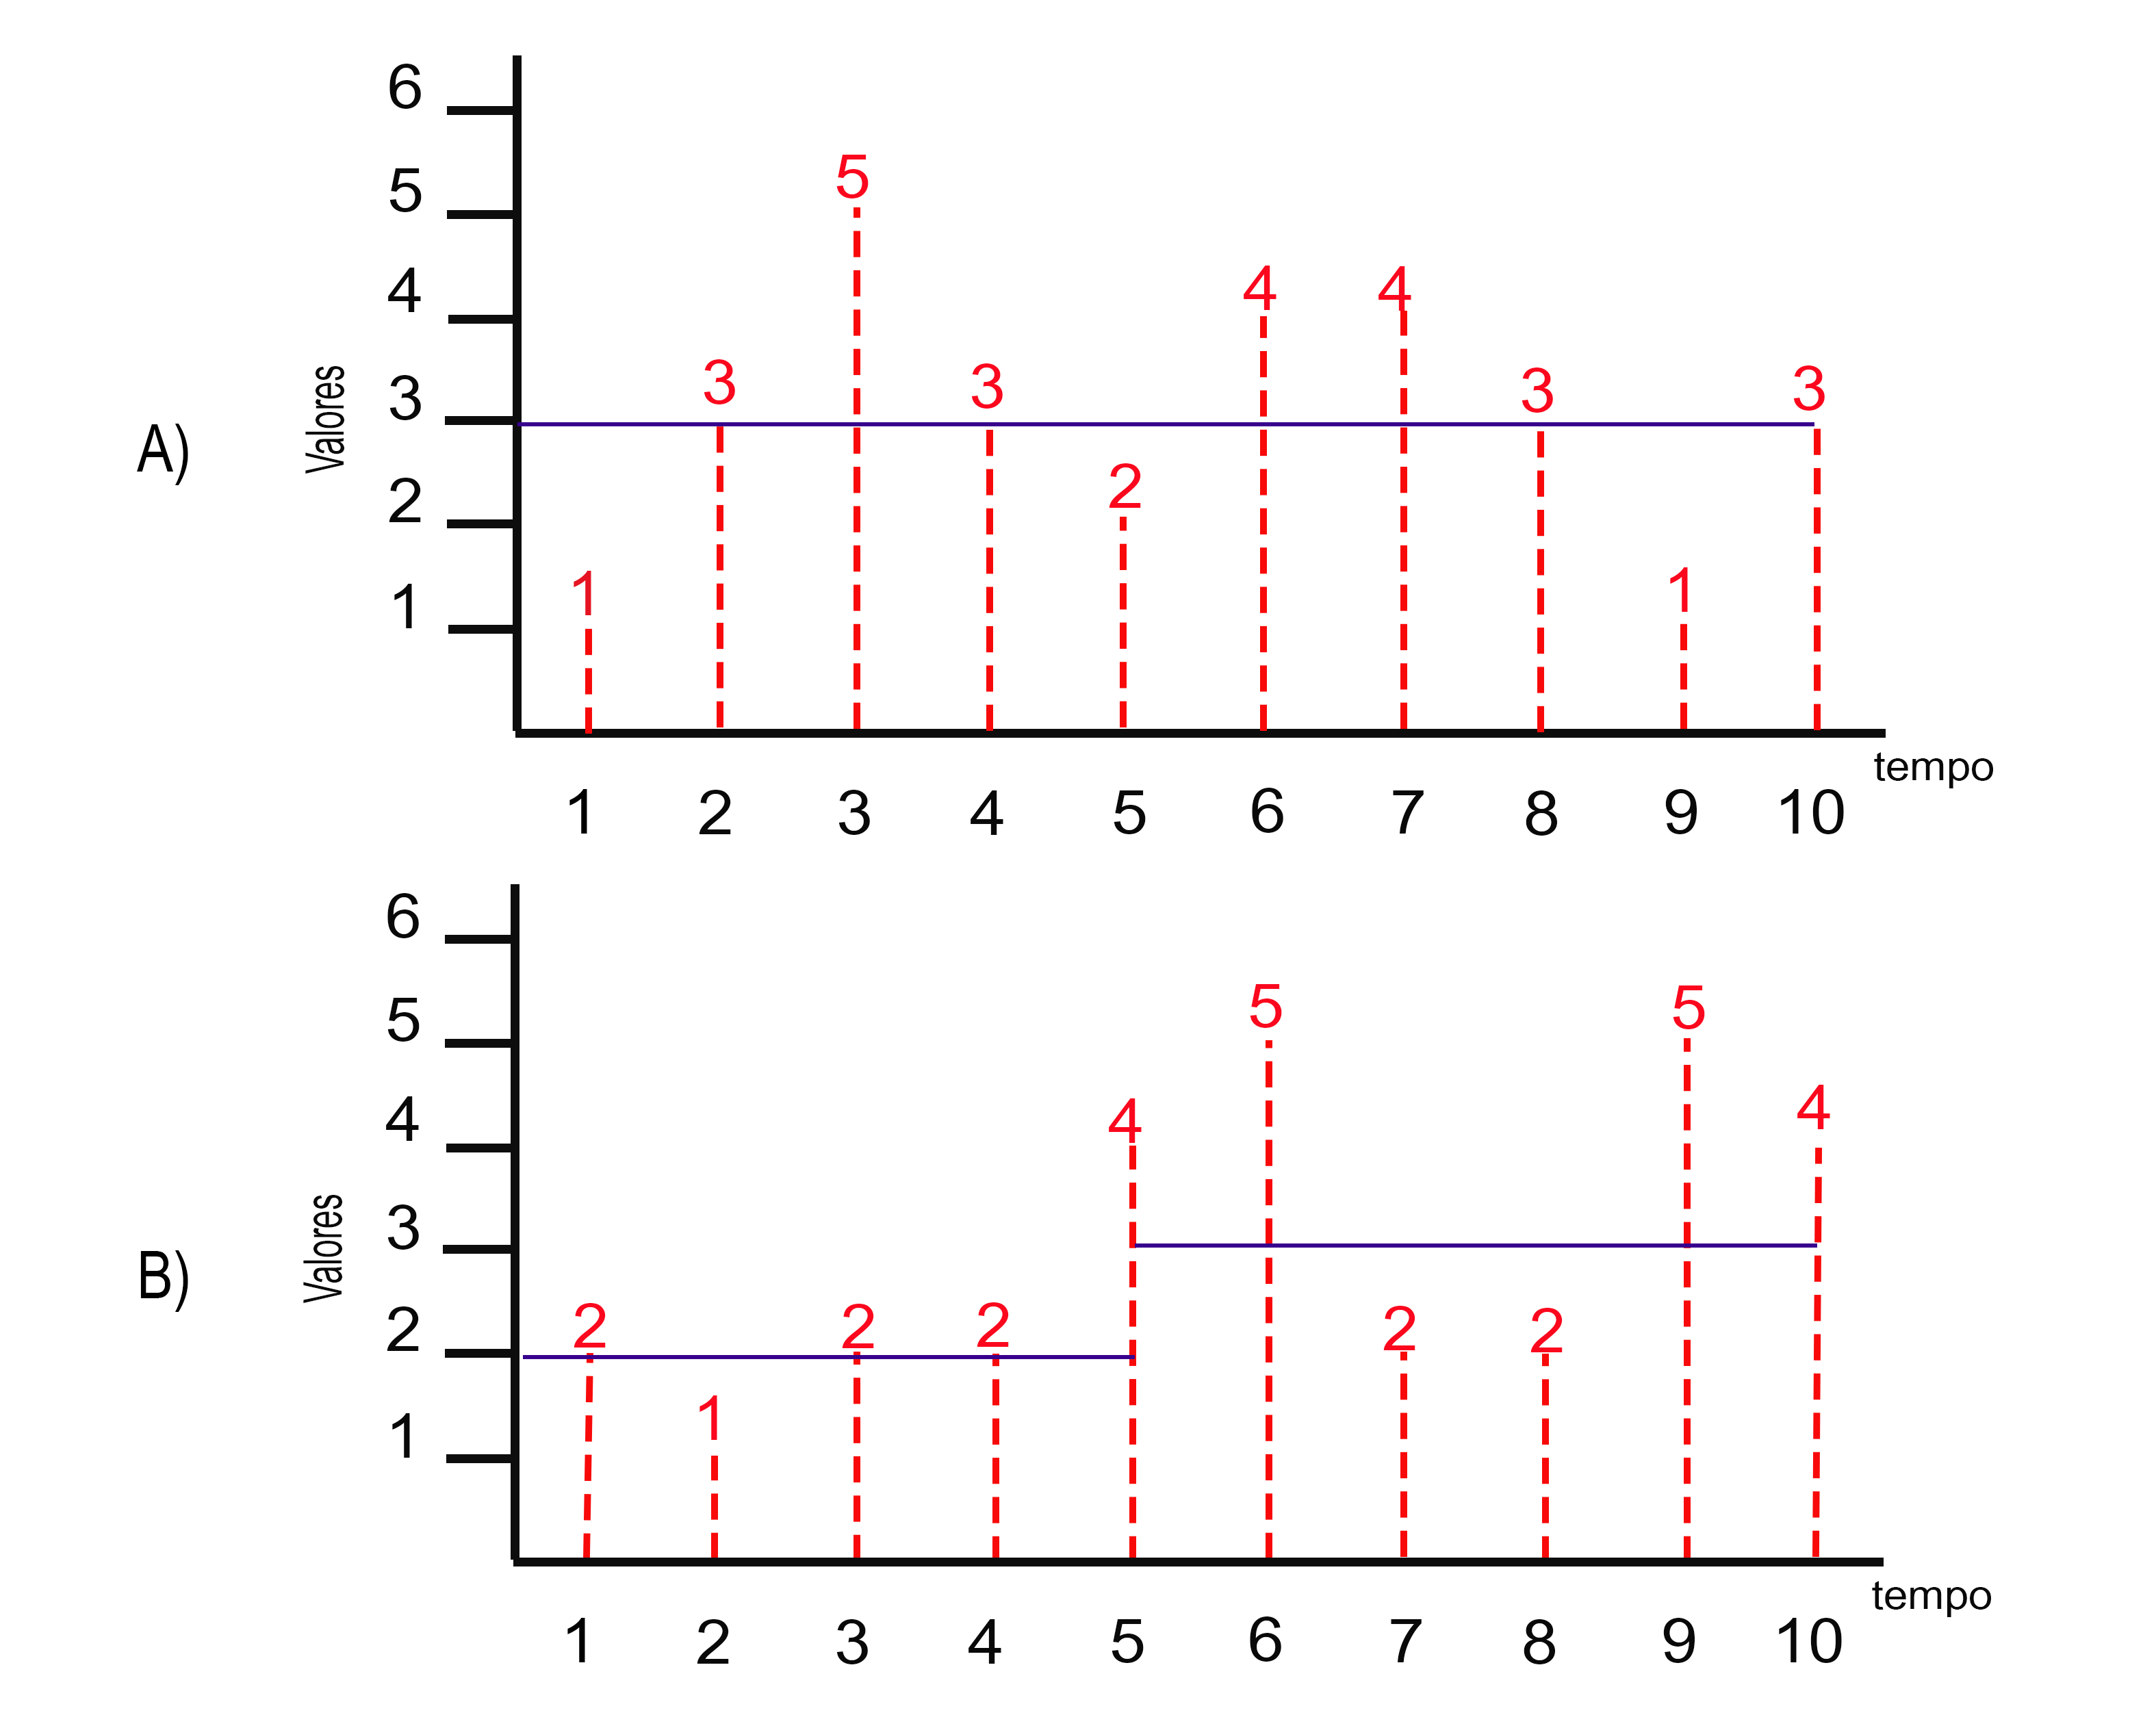
\includegraphics[scale=0.5]{./Capitulo_1/Serie_B.png}	
	\caption{Série de números gerados. Em A) os dados foram gerados a partir de um dado tetraédrico, enquanto em B) foram gerados por um dado cúbico. Apesar dos valores médios globais serem idênticos, as médias locais são diferentes.} 
	\label{SerieB}
\end{figure}
\FloatBarrier

Apesar das médias globais serem exatamente as mesmas, as séries locais possuem distribuições distintas, com média e variância diferentes. Na verdade tanto a série B como série A poderiam ter sido geradas com o mesmo dado de seis lados. A diferença clara, quando consideramos cálculos \textbf{probabilísticos} com cálculos \textbf{estatísticos}, é que a probabilidade requer conhecimento sobre o fenômeno gerador, enquanto a estatística pretende inferir situações a partir das informações dos \textbf{dados}. Na verdade, a única informações que temos a todo momento no depósito mineral são amostras e informações indiretas como geofísica e geoquímica. 

\begin{remark}
	\textit{A decisão de observar uma configuração particular dos dados como estacionário como o resultado de uma função aleatória estacionária está fortemente ligada com a decisão de que estas amostras podem ser unidas juntas. Nenhuma destas decisões pode ser checada quantitativamente, não são certas ou erradas e nenhuma prova das suas validades é possível. No entanto podem ser julgadas como apropriadas ou não.} \citet{isaaks1989applied}
\end{remark}

Apesar de o fenômeno gerador ser completamente distinto para a metade dos dados na série B, não é custoso unir estas diferentes distribuições sobre a mesma hipótese comum. Desta forma, assumir a estacionaridade neste caso é válido, dado que não conhecemos como estas informações foram construídas. 

Em alguns casos, no entanto, não parece ser muito sábio adotar a hipótese de estacionaridade de segunda ordem. Observe a imagem da figura \ref{nonest}. A série é crescente com diferenças de valores iguais a 1 começando de um ${1,2,3,4,5}$. Se você perguntasse para uma criança qual seria o próximo número na sequência ela diria $6$. Se utilizássemos geoestatística para estimar o próximo número considerando a estacionaridade dos valores, o resultado seria $3$.  

\FloatBarrier
\begin{figure}[!htb]
	\centering
	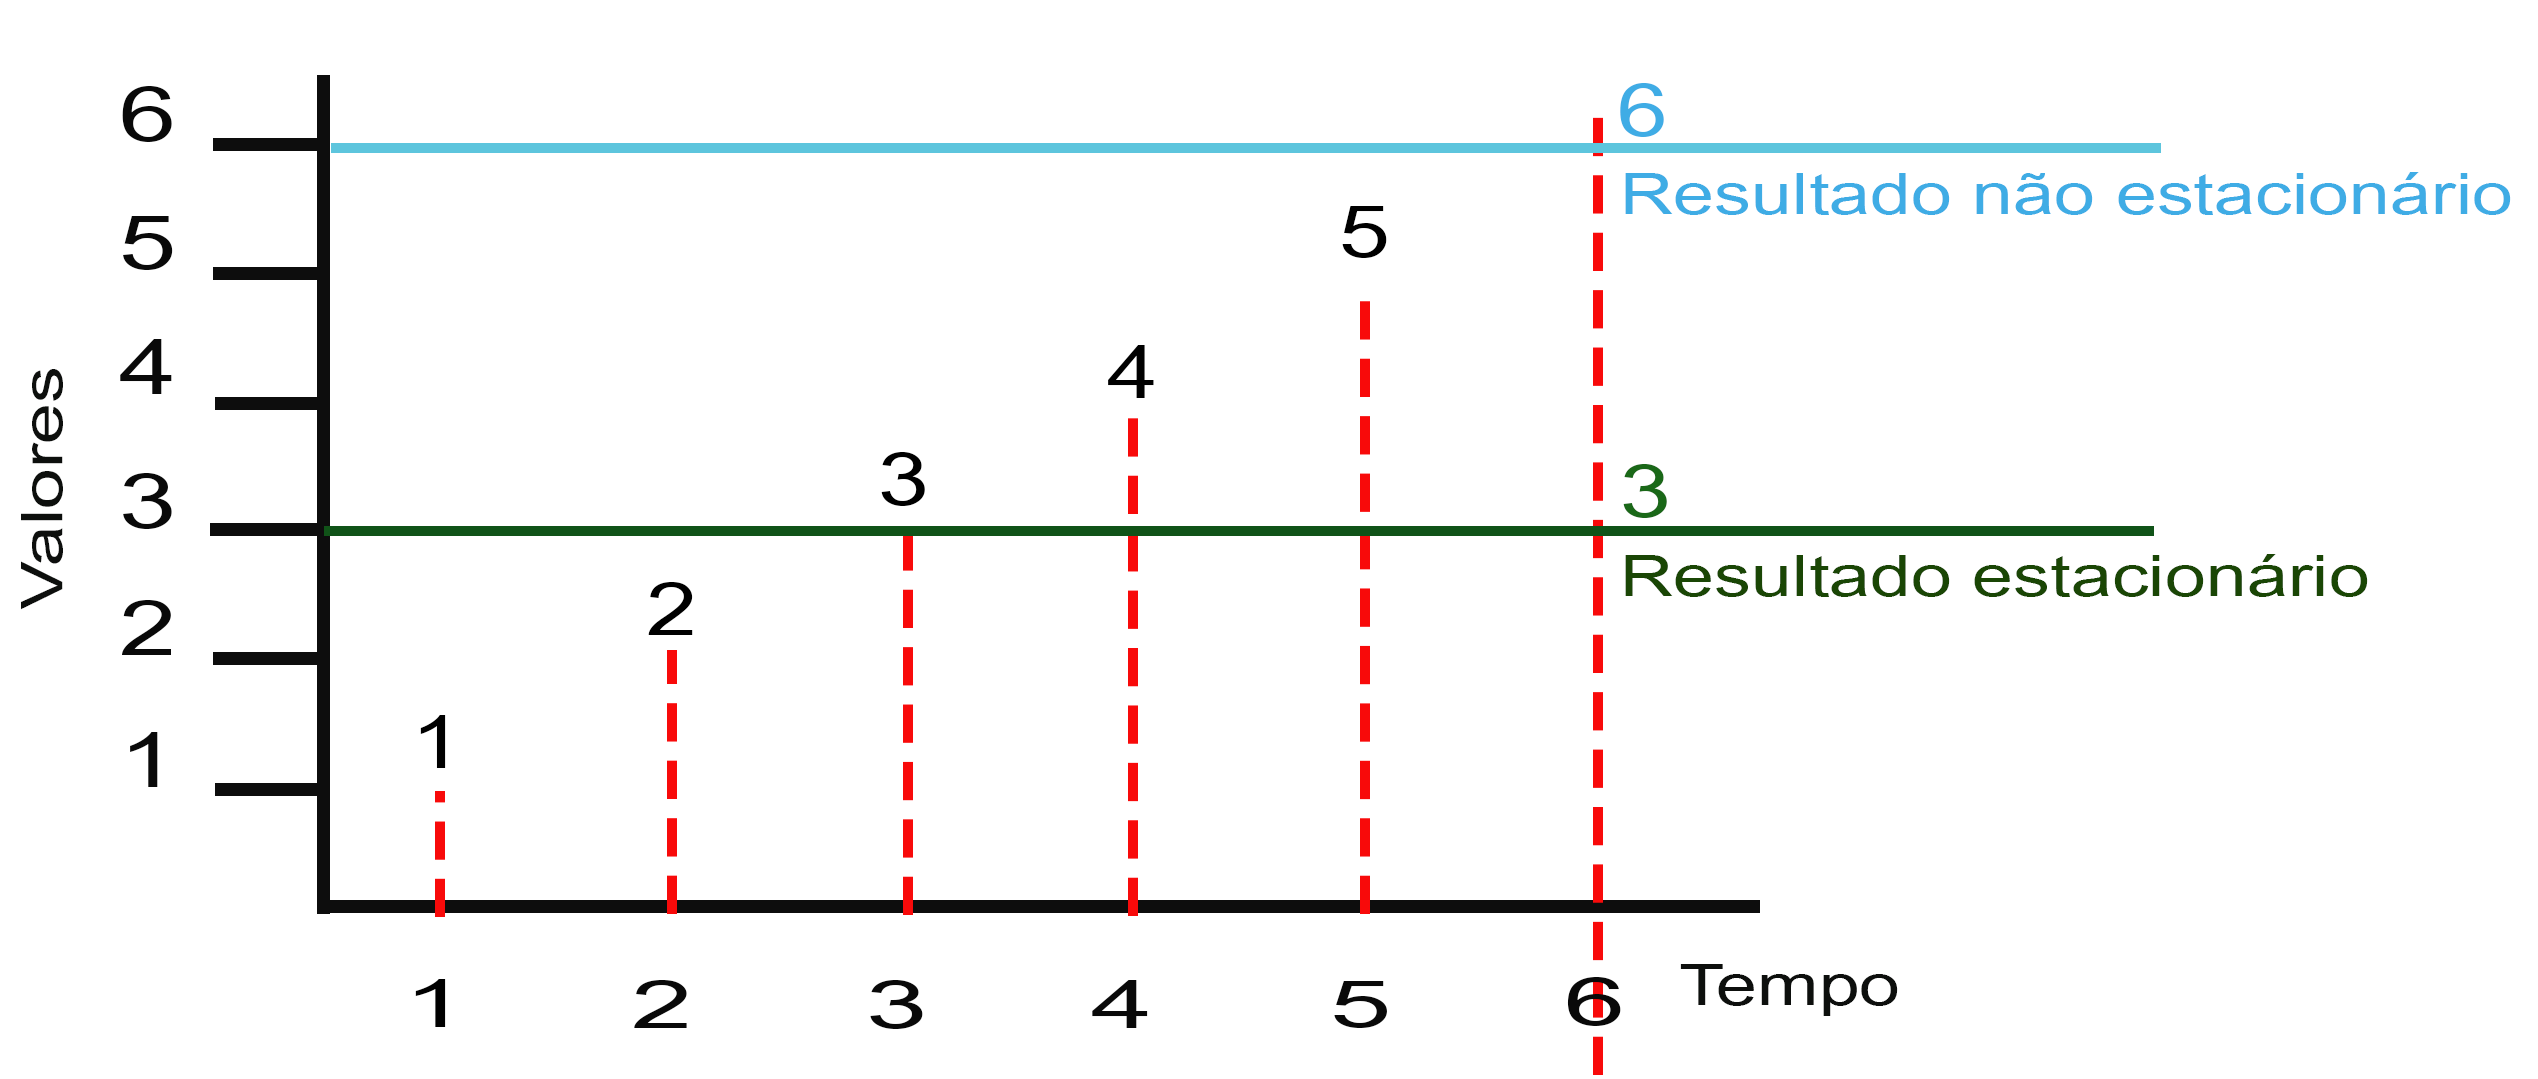
\includegraphics[width=\textwidth]{./Capitulo_1/estacionario.png}	
	\caption{Série crescente de números. O próximo número da sequência a ser estimado considerando um modelo não estacionário seria 7, enquanto para o modelo estacionário seria de apenas 6 } 
	\label{nonest}
\end{figure}
\FloatBarrier

Não parece ser sábio adotar o número 3 neste caso. Se o fenômeno gerador desta série fosse realizado por um dado, seria tão equiprovável encontrarmos o número 3 ou o número 6 na próxima realização. No entanto a informação condicionada pela série parece nos instruir com clareza que existe este padrão a partir da observação indireta dos dados, nós desconhecemos como estes dados foram gerados. Utilizando a geoestatística nos reconhecemos que existe uma \textbf{estruturação} presente nesta sequência, que condicionalmente os dados gerados parecem seguir uma ordem, e que o próximo número gerado tente a apresentar uma variação talvez equivalente como ao dos anteriores, podendo ser 4 ou até mesmo 6.

\begin{remark} 
	\textit{Uma das ideias mais importantes na geoestatística é considerar que a função aleatória gera variáveis aleatórias condicionadas ao longo do espaço. A ideia de continuidade implica que qualquer informação próxima tende a ser mais parecida do que informações muito distantes. Isto é fisicamente plausível, principalmente quando pensamos na geologia. As rochas que estão próximas tendem a possuir propriedades físico-químicas muito mais semelhantes do que quando consideramos uma distância muito grande. Por isso nos é intuitivo considerar o número estimado como 6 e não 3, pois ele representa um comportamento condicionado por medidas sucessivas, logo $Pr\{Z(x_{6}) = 6|z(x_{1}) = 1, z(x_{2}) = 2, z(x_{3}) = 3, z(x_{4}) = 4, z(x_{5}) = 5\} >  Pr\{Z(x_{6}) = 3|z(x_{1}) = 1, z(x_{2}) = 2, z(x_{3}) = 3, z(x_{4}) = 4, z(x_{5}) = 5)\}$ }
	
\end{remark}

Estes casos também são chamados na geoestatística de \textbf{deriva}, ou seja, que existem mudanças graduais na tendência dos dados. Em alguns casos é bastante lógico na mineração considerar a deriva. A topografia, por exemplo, quando analisada em determinadas escalas e situações pode ser continuamente ascendente ou descendente. Neste caso descartar a hipótese de estacionaridade de segunda ordem é sábio. 

\begin{remark}
	\textit{O custo de aceitar o uso de um modelo inapropriado é que as propriedades estatísticas dos valores estimados divergirão de modelos homólogos} \citet{isaaks1989applied}
\end{remark}

\section{Hipótese de estacionaridade} 

Como visto anteriormente podemos realizar hipóteses a respeito da função aleatória, geradora dos fenômenos geoestatísticos. Estas hipóteses são decisões que não podem ser numericamente definidas, mas que em casos convém serem julgadas, para que as estimativas não retornem valores não condizentes com a realidade. A escolha de um tipo de estacionaridade significa que adotamos um critério que considere um conjunto de dados com um comportamento \textbf{homogêneo}. Uma das hipóteses utilizada pela geoestatística mais importantes, e que não constitui critério de escolha, é a chamada de \textbf{hipótese estrita}. Diferentemente da hipótese de estacionaridade de segunda ordem, esta é adotada automaticamente quando se opta por um método geoestatístico e não é passível de decisão. A principal ideia da estacionaridade estrita é que o fenômeno é homogêneo em uma mesma direção no espaço, sendo \textbf{invariante por translação}. 

\begin{remark}
	\textit{A ideia de areia em um jarro é uma boa imagem da estacionaridade de uma função aleatória em três dimensões, pelo menos enquanto a areia estiver bem ordenada (de outra forma se esta jarra vibrar, os grãos finos se depositarão na base, criando não estacionaridade vertical)} \citet{chiles2009geostatistics}
\end{remark}

Uma forma geométrica de pensarmos na hipótese estrita é pelo uso de fractais. Fractais são figuras geométricas autosimilares, em que cada um de seus componentes carregam características da informação como um todo. A figura \ref{fractal} representa um fractal. Estas formas autosimilares são muito comuns na natureza, seja no padrão desenhado por cristais de gelo, pela forma das plantas e principalmente nas rochas. A geologia em pequena escala muitas vezes é uma repetição que se traduz em grande escala. 


\FloatBarrier
\begin{figure}[!htb]
	\centering
	\includegraphics[scale=0.6]{./Capitulo_1/fractal.png}	
	\caption{Fractal gerado a partir da repetição sistemática de estruturas cada vez menores. } 
	\label{fractal}
\end{figure}
\FloatBarrier

\begin{proposition}
	\textit{Todo o conhecimento humano somente advém do entendimento de padrões. As diferentes disciplinas, sejam elas humanas, biológicas ou exatas, apenas diferenciam quanto ao objeto de estudo. Não há diferença nenhuma entre um físico que entende padrões referentes ao movimento de planetas, um linguista que estuda o padrão de idiomas, um historiador que verifica padrões no tempo, ou um matemático que verifica o padrão das formas. A natureza também age desta forma, pois esperamos acordar no dia seguinte com o sol sobre as montanhas. Até mesmo dentro de fenômenos que parecem ser puramente aleatórios, podemos encontrar motivos pelos quais podemos entender padrões. Independente de fenômenos serem estacionários ou não estacionários, a geoestatística procura simplesmente estas formas no espaço, representações que apesar de não serem físicas, são mímicas da natureza da existência destes fenômenos}
\end{proposition}
 
Esta repetição de comportamentos em uma direção leva a seguinte defnição matemática. Um fenômeno dito estacionário estrito significa que $Pr\{Z(x_{1}) < z(x_{1}), Z(x_{2}) < z(x_{2}),..., Z(x_{k}) < z(x_{k})\} = Pr\{Z(x_{1 + h}) < z(x_{1 + h}), Z(x_{2 + h}) < z(x_{2 + h}), ...,Z(x_{k + h}) < z(x_{k  + h})\}$, sendo $h$ um vetor de direção determinada. A hipótese de estacionaridade estrita significa que exite um grau de repetição no comportamento da variável ao longo de uma direção, no entanto, o fenômeno espacial pode apresentar deriva. Outra questão a ser abordada é o fato de que a adoção da estacionaridade é dependente da escala analisada. Um fenômeno considerado não estacionário pode assumir comportamento estacionário local. Obeserva a série de dados representada pela figura \ref{temd}. Quando analisado o comportamento global da função aleatória esta apresenta nitidamente uma tendência nos dados, no entanto, quando considerada uma escala menor do vetor $h$, este mesmo comportamento pode ser tomado como estacionário. Este fenômeno também é chamado de \textbf{quasi estacionário}.


\FloatBarrier
\begin{figure}[!htb]
	\centering
	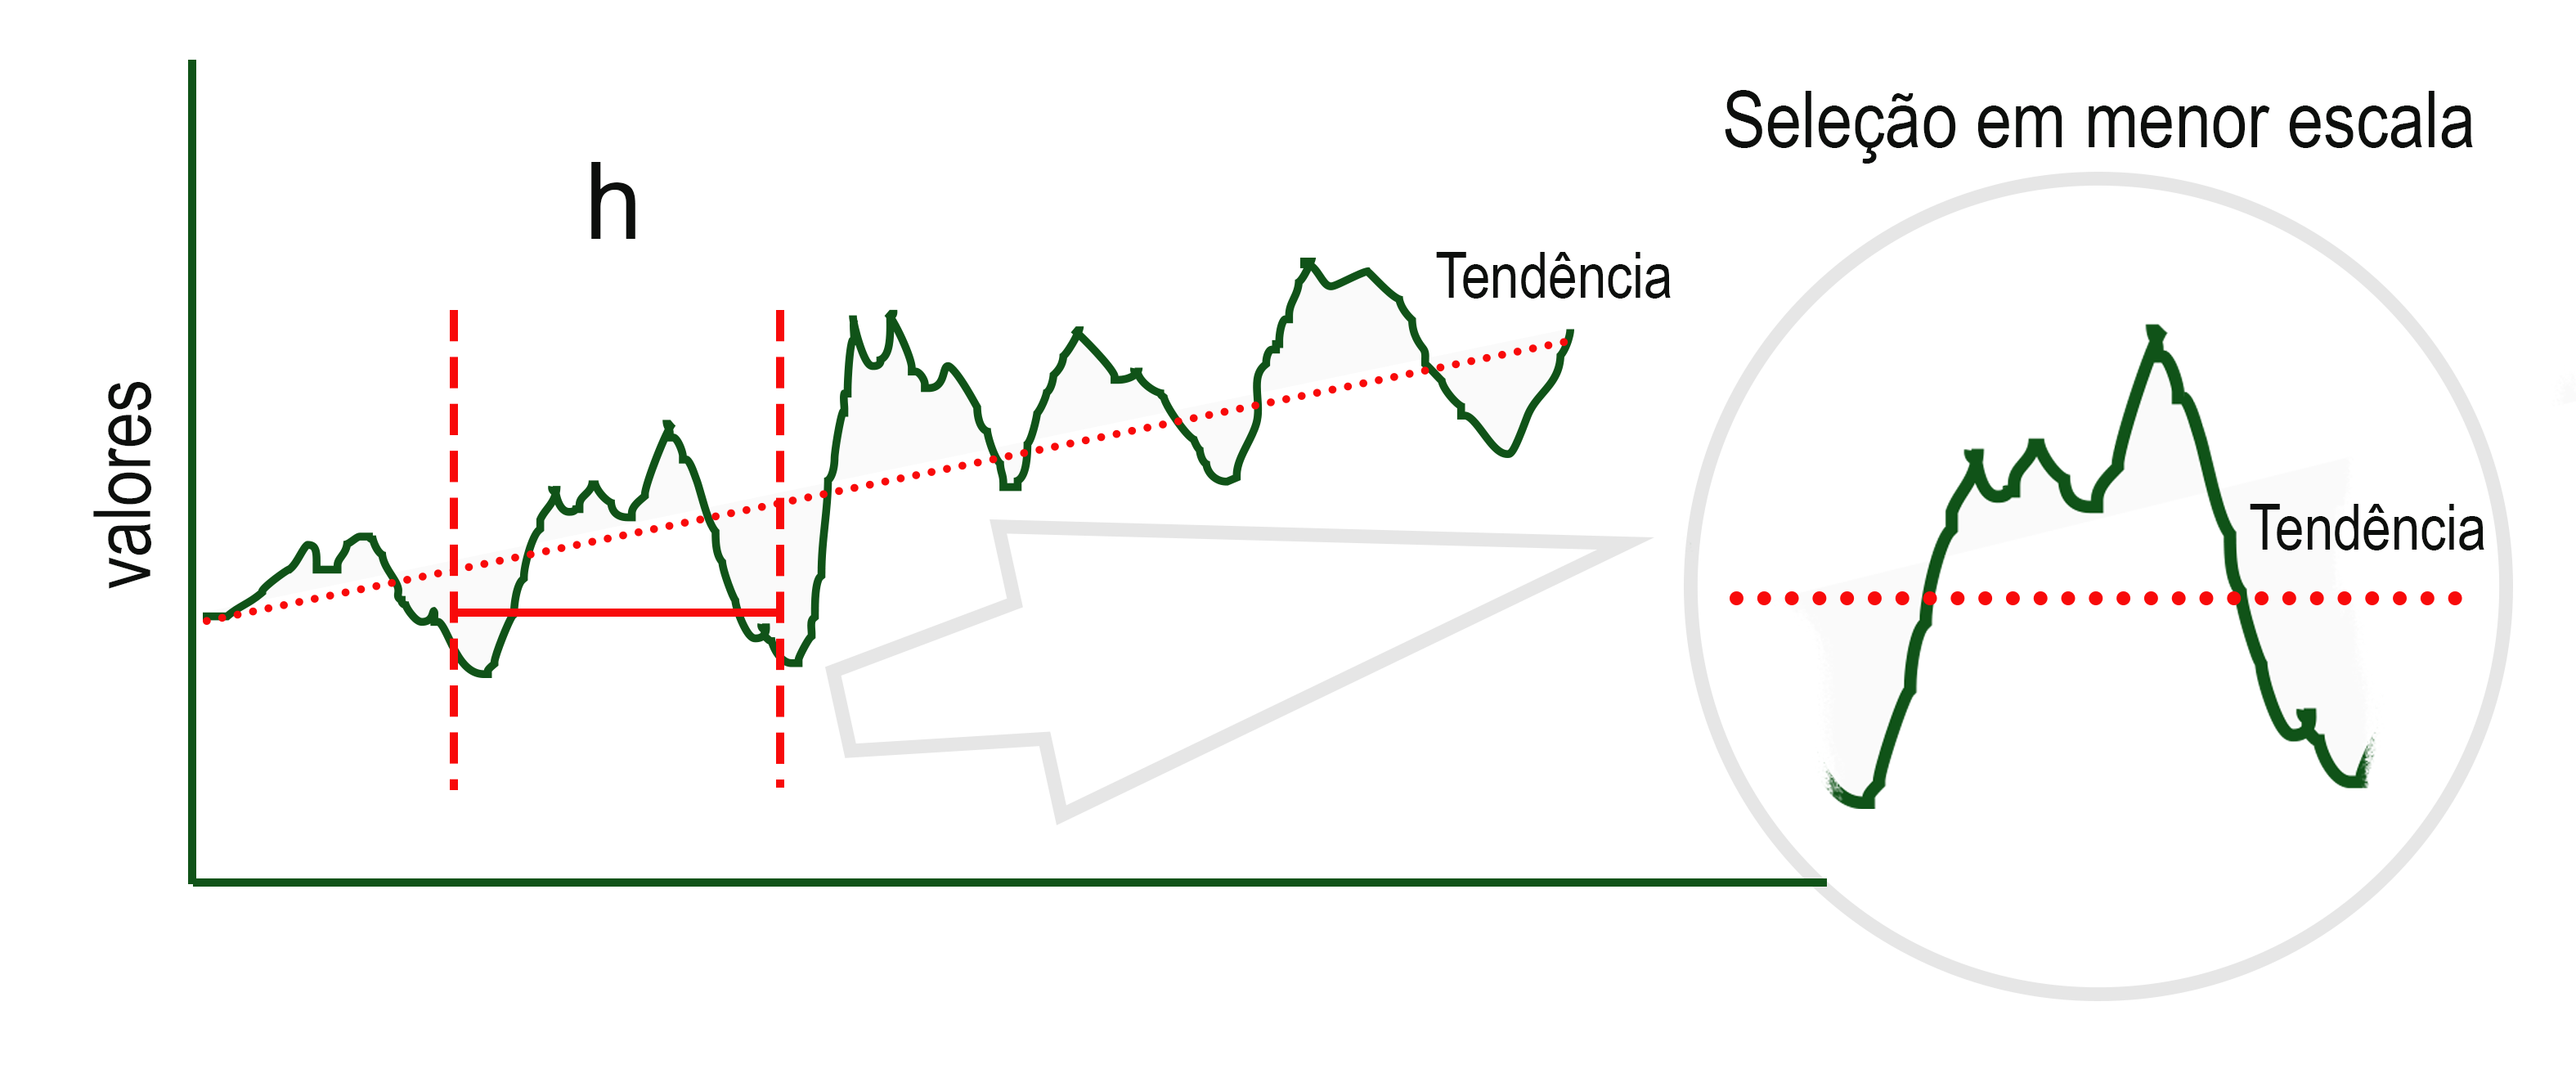
\includegraphics[scale=0.6]{./Capitulo_1/temd.png}	
	\caption{Comportamento analisado de uma série não estacionária quando analisada em um domínio global, e estacionária quando analisada em um domínio menor de comprimento $h$. } 
	\label{temd}
\end{figure}
\FloatBarrier

\begin{proposition}
	\textit{Uma das maiores contribuições da geoestatística para a ciência talvez tenha sido a concepção de que os fenômenos podem ser dependentes da escala analisada. Dependendo da observação nossas hipóteses a respeito do fenômeno podem mudar. Isto é fisicamente compatível com a ideia da geologia. Analisar um depósito mineral em uma grande extensão de área, com toda a certeza é diferente quando observamos variações de tamanho centimétrico. A própria observação da Terra quando vista do espaço apresenta belos tons azuis e brancos, mas quando aproximamos a escala de uma região do tamanho de um país, notamos como nossa visão é diferente e muito mais variável.} 
\end{proposition}

A hipótese de estacionaridade estrita é uma hipótese realizada sobre a característica do fenômeno, não dos resultados das amostras. A hipótese de estacionaridade de segunda ordem, no entanto, é uma hipótese relacionada com os \textbf{momentos estatísticos} do fenômeno. A principal ideia dos momentos estatísticos é que eles representam de alguma forma o resumo da distância entre os dados, desta forma quando pensamos na estacionaridade intrínseca, ou na estacionaridade de segunda ordem, pensamos na possível homogeneidade da distância entre os dados. 

O conceito de \textbf{estacionaridade intrínseca}, desta forma, apresenta também outra forma de conceber esta homogeneidade, quando estabelecemos que uma variação $Y_{h}(x) = Z(x+h) -Z(x)$ é estacionária de segunda ordem. Em outras palavras dizemos que existe homogeneidade quando consideramos a diferenças entre variáveis aleatórias geradas pela função aleatória. Segundo \citet{chiles2009geostatistics}, se a hipótese de estacionaridade intrínseca pode ser considerada e não ocorre uma tendência, então o valor médio da função aleatória é constante, e o valor esperado de $Y_{h}(x)$ é zero. 

\section{Momentos estatísticos} 

Como dito anteriormente, momentos estatísticos são representações da distância entre dados. As medidas de distância, podem ser por exemplo, medidas da tendência central dos dados ou medidas da dispersão destes dados. A figura \ref{moment} representa os conceitos de \textbf{tendência central}  e de \textbf{dispersão}. 

\FloatBarrier
\begin{figure}[!htb]
	\centering
	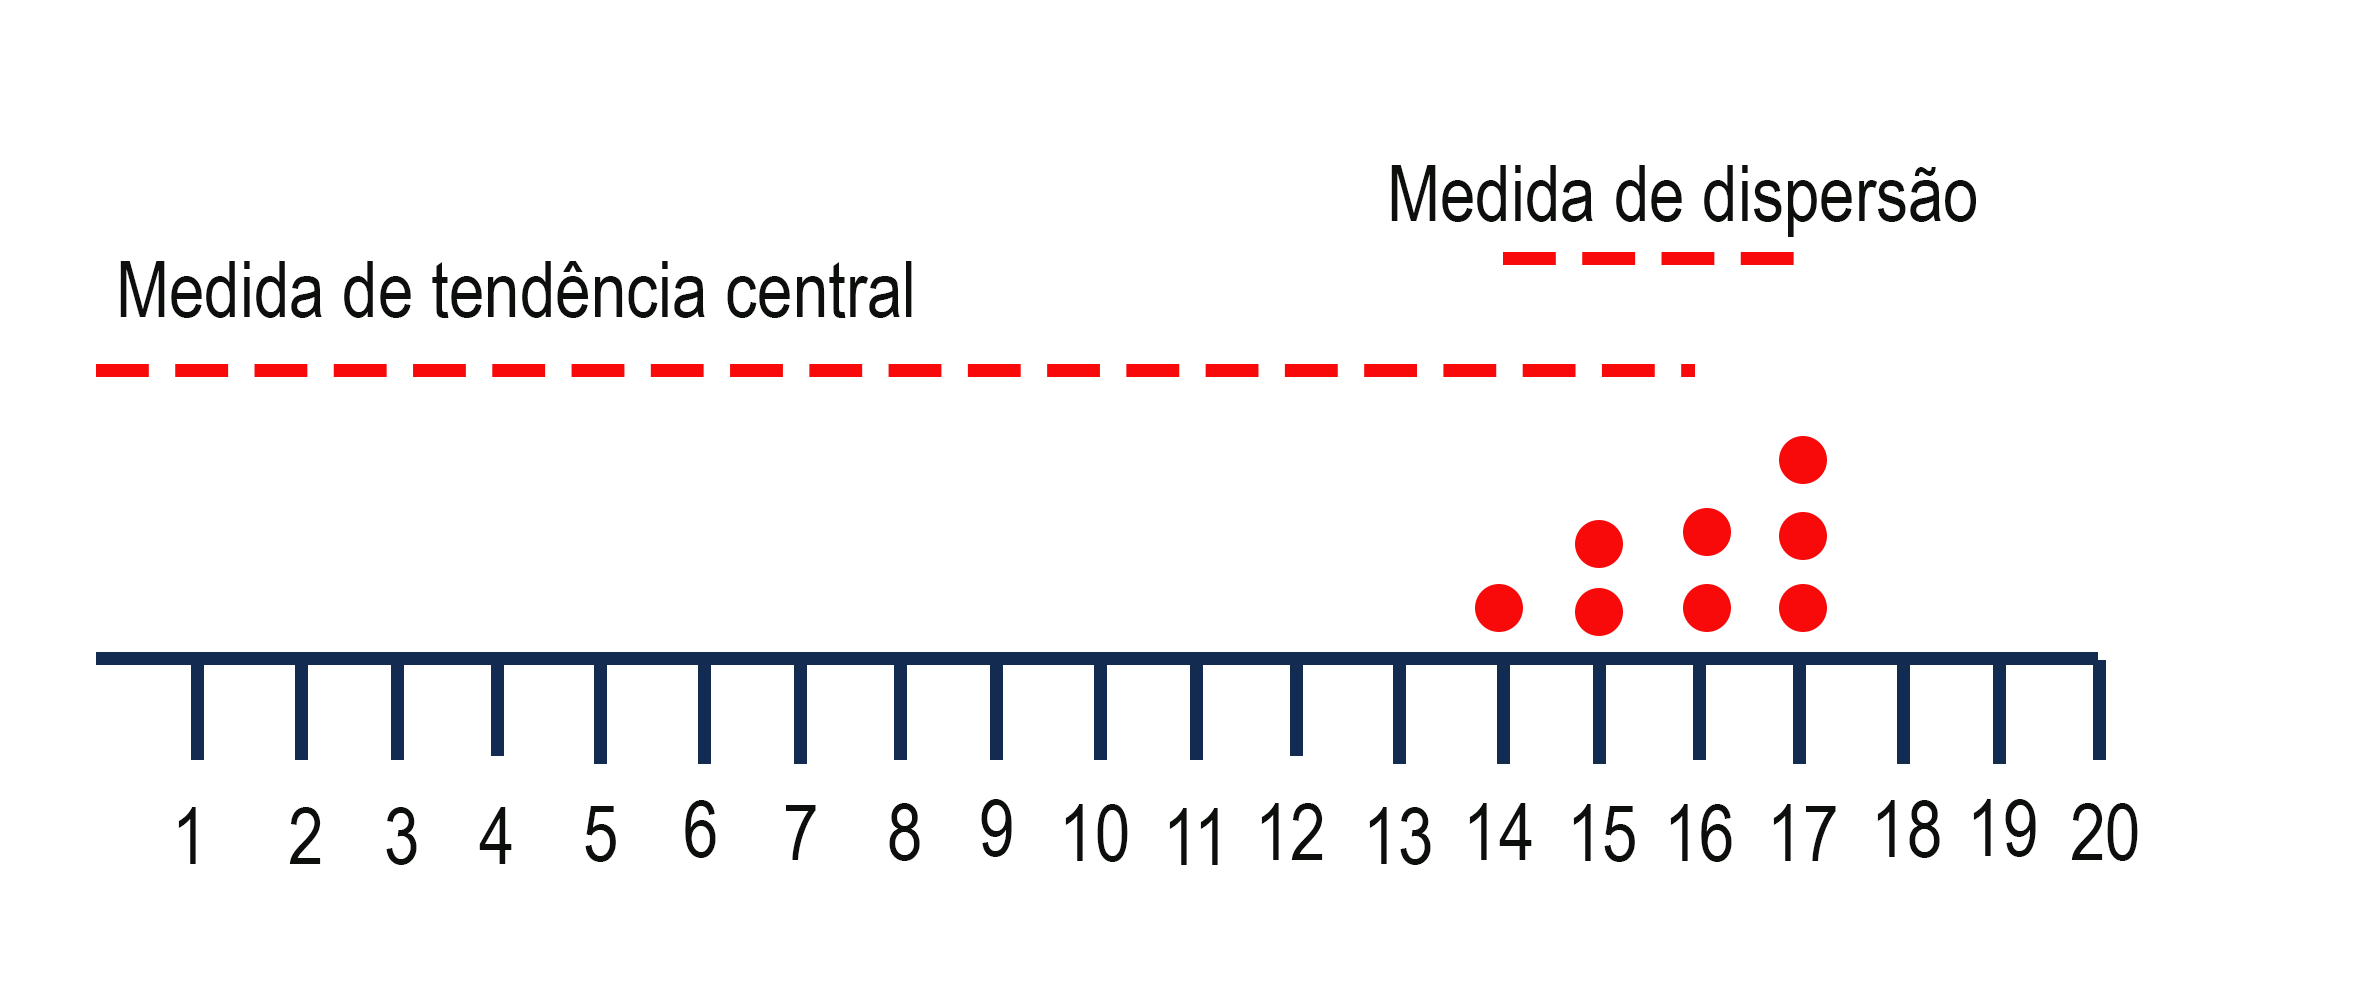
\includegraphics[scale=0.8]{./Capitulo_1/moment.png}	
	\caption{Exemplos de momentos estatísticos para um conjunto de dados. O valor médio representa o quão distante está o centro dos dados, enquanto a dispersão apresenta quão agregados estão estes dados. } 
	\label{moment}
\end{figure}
\FloatBarrier

A principal medida da distância do centro dos dados é chamada de \textbf{esperança matemática}, e pode ser representada para variáveis contínuas como. 

\begin{equation}\label{eq1:Valor_esperado}
E\left(Z\right)= \int_{z = -\infty}^{z =+\infty} z f\left(z\right)dz
\end{equation}

No caso de variáveis discretas, podemos determinar a esperança matemática como 

\begin{equation}\label{eq2:Valor_esperado_discreto}
E\left(Z\right)= \sum_{i=-\infty}^{+\infty}Pr\left(z_i\right)z_i
\end{equation}

Muitas vezes há confusões ao se dizer que a esperança matemática representa o valor mais provável que determinada variável pode possuir. No entanto, a esperança matemática é simplesmente uma medida da distância do centro dos dados, sendo que este centro pode ser pouco provável ou nem mesmo existir. Observe a figura \ref{moment2}. A esperança matemática neste caso representa o centro de uma distribuição com probabilidade muito baixa de ocorrência.

\FloatBarrier
\begin{figure}[!htb]
	\centering
	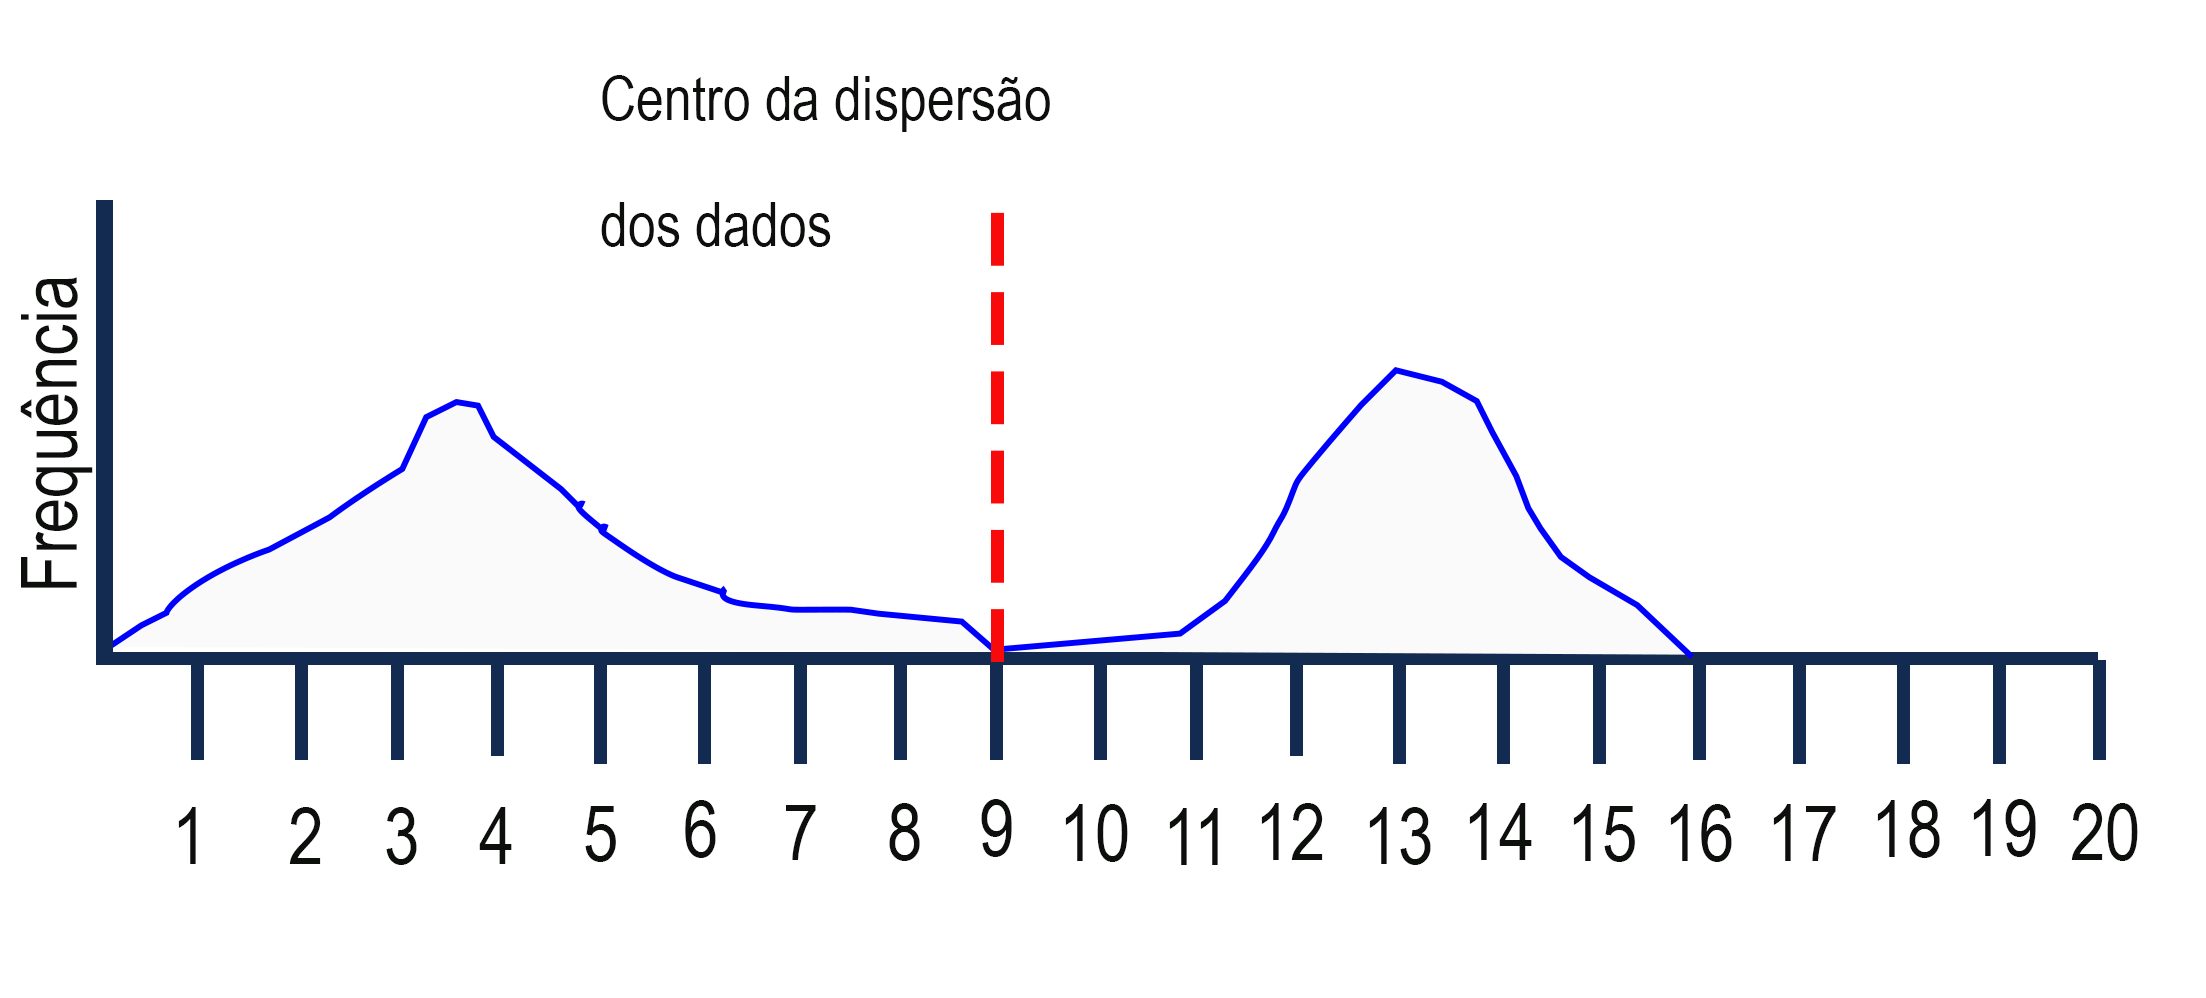
\includegraphics[scale=0.6]{./Capitulo_1/moment2.png}	
	\caption{Exemplo da esperança matemática de uma distribuição multimodal. O valor da probabilidade para este centro de dispersão é praticamente nulo. } 
	\label{moment2}
\end{figure}
\FloatBarrier

O que de fato ocorre é que os centros de dispersão dos dados da maioria dos problemas de engenharia não são multimodais, ou seja, apresentam vários picos nas distribuições de densidade de probabilidade com na figura. Neste caso a esperança matemática pode representar os valores mais prováveis de ocorrência da dispersão dos dados.

Pela definição da esperança matemática, algumas propriedades podem ser diretamente derivadas. A multiplicação da variável aleatória $Z$ por um valor constante $c$, implica na seguinte condição. 

\begin{equation}\label{eq3:Propesperancamatematica}
E\left(cZ\right)= cE\left(Z\right)
\end{equation}

O valor esperado de uma variável aleatória constante pode ser relacionada pela seguinte propriedade

\begin{equation}\label{eq4:Propesperancamatematica2}
 E(c) = c
\end{equation}

A demonstração, na verdade é muito simples, já que advém da própria definição de esperança mamtemática


\begin{proof} 
	Valor esperado de uma constante é igual a ela mesma
	\begin{align*}
	&E\left(c\right)= \sum_{i=-\infty}^{+\infty}Pr\left(c\right)c \\
	& E\left(c\right)= c\sum_{i=-\infty}^{+\infty}Pr\left(c\right) \\
	& Como: \sum_{i=-\infty}^{+\infty}Pr\left(c\right) = 1 \\
	& E\left(c\right)= c
	\end{align*}
\end{proof}

A partir da definição da esperança matemática como uma medida de centralidade da distribuição dos dados, podemos derivar outros momentos representando diferentes distâncias desta distribuição. Os diferentes momentos matemáticos podem caracterizar diferentes distâncias relativas à \textbf{centralidade} , \textbf{dispersão} , \textbf{assimetria} , \textbf{forma}. A geoestatística, na verdade, foca sua análise principalmente nos momentos de primeira e segunda ordem.

\begin{remark}
	\textit{Em aplicações da mineração, a lei de probabilidades espacial nunca é requerida, principalmente porque os dois primeiros momentos da função são suficientes para providenciar uma solução aproximada para muitos problemas encontrados} \citet{journel1978mining}
\end{remark}

Outro momento estatístico importante é a variância, definida como o momento de segunda ordem centrado. A variância pode ser considerada como uma medida de dispersão, demonstrada por

\begin{equation}\label{eq4:CapVariancia1}
Var\left(Z\right)= E\left( Z - E\left( Z\right) \right)^2
\end{equation} 

Esta forma tradicional da variância pode ser substituída por outra representação a partir de 

\begin{equation}\label{eq4:CapVariancia2}
Var\left(Z \right)= E(Z^2) - E(Z)^2
\end{equation} 

fA prova desta relação também é facilmente demonstrada a partir das propriedades da esperança matemática e pela definição da variância.

\begin{proof} 
	Relação entre as equações \ref{eq4:CapVariancia1} e \ref{eq4:CapVariancia2}
	\begin{align*} 
	&Var\left( Z \right)= E\left( Z -E(Z) \right)^2  \\
	&Var\left(Z \right)= E\left( Z^2 -2ZE\left( Z\right)+ E(Z)^2 \right) \\
	&Var\left(Z \right)= E(Z^2) -E(2ZE(Z)) +E(Z)^2  \\
	&Var\left(Z \right)= E(Z^2) -2E(Z)E(Z) +E(Z)^2  \\
	&Var\left(Z \right)= E(Z^2) -2E(Z)^2 +E(Z)^2 \\
	&Var\left(Z \right)= E(Z^2) - E(Z)^2
	\end{align*}
\end{proof}

 Os momentos estatísticos de primeira e segunda ordem, representados pela esperança matemática e pela variância representam medidas tomadas de uma única variável aleatória. Para relacionar diferentes variáveis aleatórias utilizamos comumente a \textbf{covariância}, esta representada pela similaridade entre duas variáveis aleatórias. Considere as variáveis aleatórias Z e Y. Podemos representar a covariância pela seguinte relação
 
 \begin{equation}\label{eq6:CapCorrelacao}
 Cov\left(Z,Y\right)= E\left( (Z-E(Z)) (Y-E(Y)) \right)
 \end{equation}
 
 Se as variáveis $Z$ e $Y$ apresentam médias idênticas iguais a $m$, então a covariância pode ser representada por 
 
  \begin{equation}\label{eq6:CapCorrelacao}
 Cov\left(Z,Y\right)= E\left( ZY \right) - m^{2}
 \end{equation}
 
 A prova desta relação pode ser facilmente obtida 
 
 \begin{proof}
 	Relação da Covariância considerando médias idênticas iguais a m
 	\begin{align*}
 	&Como:  E(Z) = E(Y) = m  \\
 	&Cov\left(Z,Y\right)= E\left( (Z-m) (Y-m) \right)\\
 	&Cov\left(Z,Y\right)= E\left( ZY - Zm - Ym +m^2 \right)\\
 	&Cov\left(Z,Y\right)= E(ZY) - E(Zm) - E(Ym) +E(m^2)\\
 	&Cov\left(Z,Y\right)= E(ZY) - mE(Z) - mE(Y) +E(m^2)\\
 	&Cov\left(Z,Y\right)= E(ZY) - m^2 - m^2 +m^2\\
 	&Cov\left(Z,Y\right)= E(ZY) - m^2
 	\end{align*}
 \end{proof}

Se as variáveis Y e Z forem idênticas, a covariância entre as duas variáveis aleatórias é equivalente a variância. A prova pode ser demonstrada por

\begin{proof}
	Prova de que a covariância é idêntica a variância para Z=Y
	\begin{align*}
	&Como: Y=Z \rightarrow Cov(Z,Y) = Cov(Z,Z)  \\
	&C\left(Z,Z\right) = E\left( (Z-E(Z))(Z-E(Z)) \right) \\
	&C\left(Z,Z\right) = E\left( Z-E(Z) \right)^2 \\
	&C\left(Z,Z\right) = Var(Z) \vee   Var(Y) \\
	\end{align*}
\end{proof}

\section{Ergocidade} 

A ergocidade é uma das propriedades mais importantes da funcão aleatória. A ideia é de que cada vez ao qual analisamos um volume maior no espaço, a tendência é que o valor médio deste volume se aproxime cada vez mais do valor médio do fenômeno. Matematicamente podemos definir a propriedade da ergocidade como 

\begin{equation}
\lim_{V\rightarrow \infty}\frac{1}{|V|}\int_{x \in V}Z(x)dx = m 
\end{equation}

Em que $|V|$ é o volume considerado e $m$ o valor da média do fenômeno. 
\begin{definition}[Ergocidade]
	\textit{A Ergocidade pode ser caracterizada como a propriedade da função aleatória de convergência dos valores médios se aproxime a um valor constante $m$, de acordo com um domínio $V$ considerado.}
\end{definition}

Alguns fenômenos tendem a apresentar dispersões infinitas, crescentes de acordo com o desenvolvimento da função aleatória. Estes fenômenos podem apresentar dispersão infinita, tal como o fenômeno de movimento browninano. 

\section{Homocedasticidade e heterocedasticidade}

Além do comportamento da estacionaridade dos valores médios da função aleatória, também é importante qualificar os fenômenos geoestatísticos a partir do comportamento da variância. A figura \ref{etero}, por exemplo, demonstra um comportamento crescente da variância de acordo com o desenvolvimento da série.

\FloatBarrier
\begin{figure}[!htb]
	\centering
	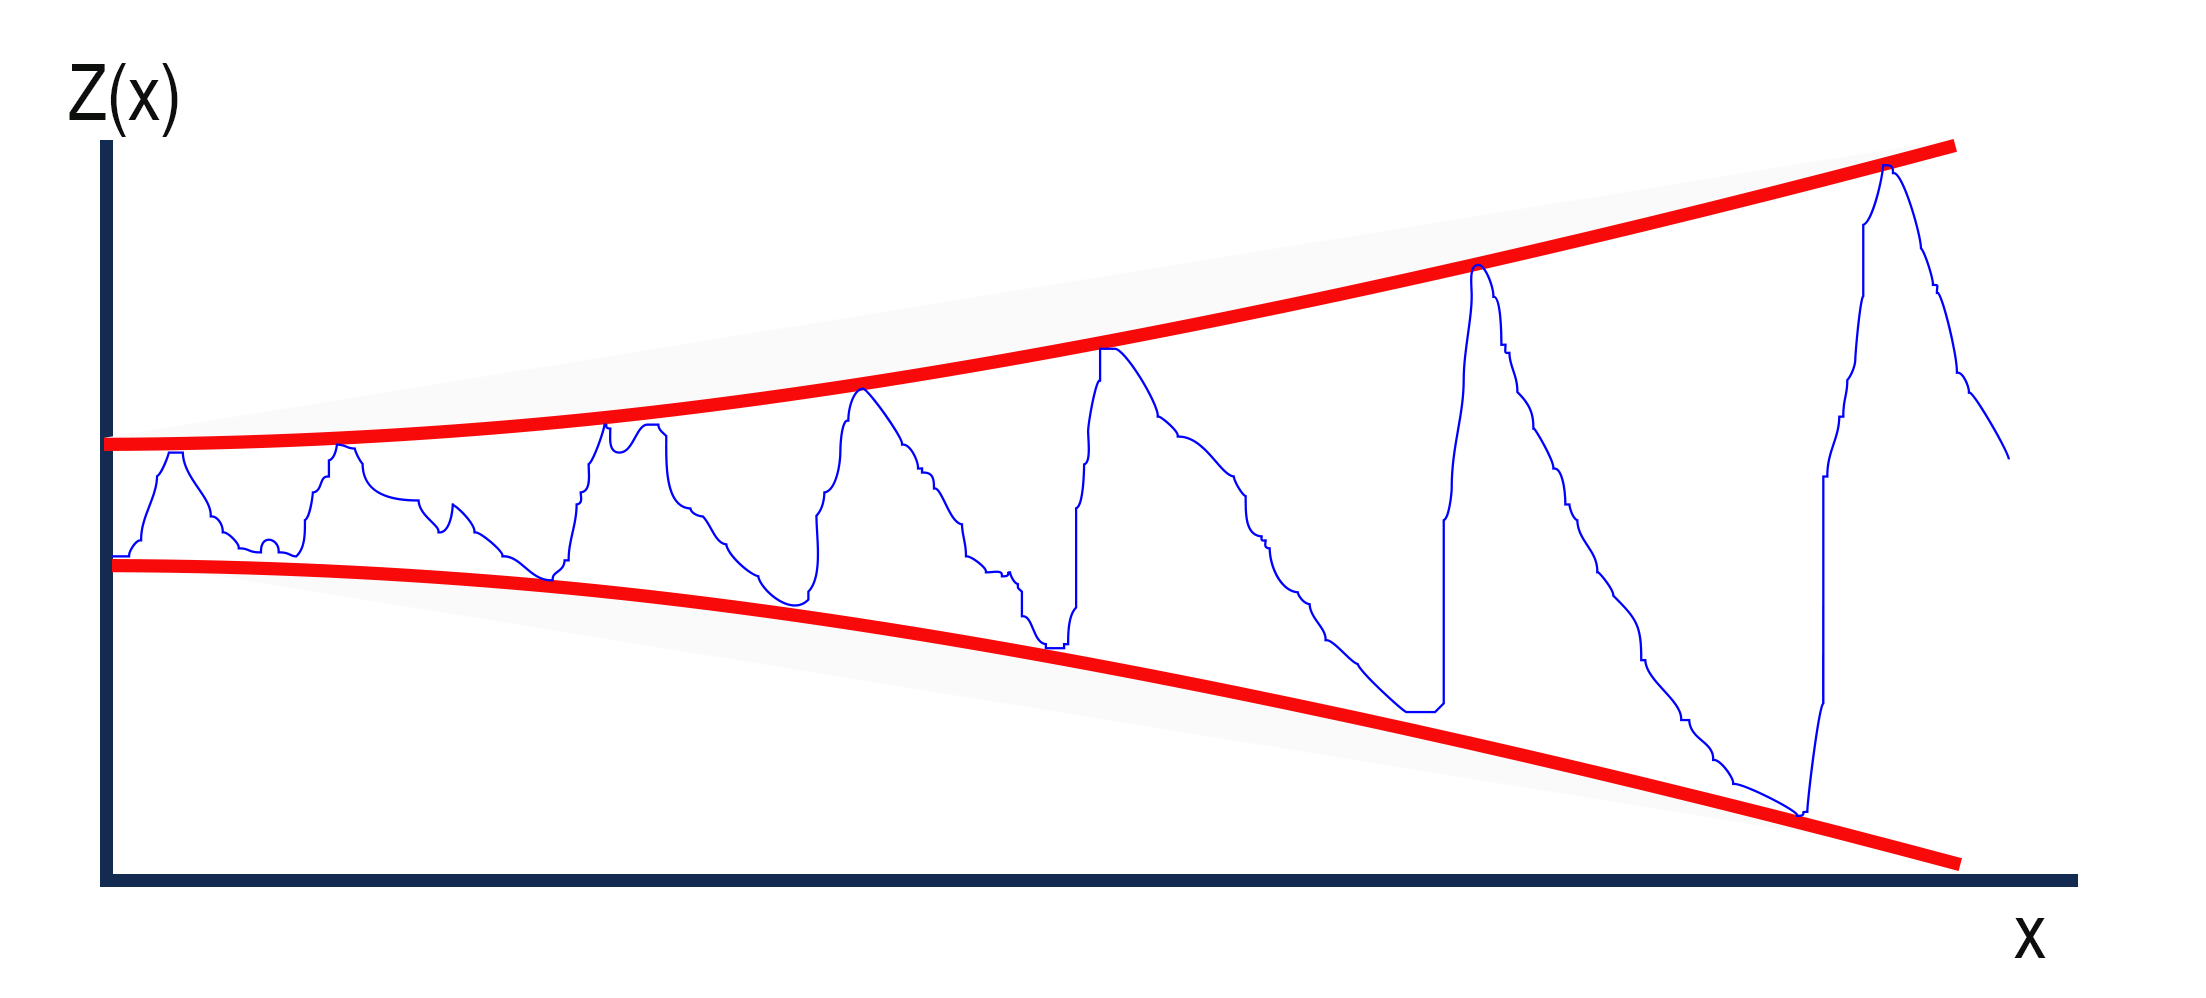
\includegraphics[width=\textwidth, height=4cm]{./Capitulo_1/heterocedasticidade.png}	
	\caption{Fenômeno de heterocedasticidade representando variabilidade infinita da função aleatória } 
	\label{etero}
\end{figure}
\FloatBarrier

 Estes fenômenos são chamados de \textbf{heterocedásticos}, e aumentam a variabilidade de acordo com o incremento da direção. Fenômenos constantes quanto a dispersão local são chamados de \textbf{homocedásticos}

\begin{definition}[homocedasticidade]
	A hipótese de homocedasticidade,  igual \textit{(homo)} dispersão \textit{(scedasticidade)}, implica que a variância da função aleatória é constante para todo e qualquer ponto $x$ representado no domínio $D$. A heterocedasticidade, no entanto, implica que a variância aumenta ao longo da função aleatória.
\end{definition}

\section{Relação Volume Variância}

Na geoestatística, a variável aleatória se manifesta em todos os pontos no espaço. No entanto, nem sempre é possível reconhecer a variável em um suporte pontual, e para fins de engenharia precisamos entender a variável aleatória dentro de domínios específicos, sejam eles os domínios da amostra, na unidade seletiva de lavra, ou dentro de um domínio de estimativa. Na geoestatística clássica, apenas se determina os \textbf{valores esperados} destas variáveis dentro de um domínio, principalmente os de primeira e segunda ordem, não se importando com o reconhecimento das distribuições locais. 

O processo de se determinar volumes esperados dentro de um domínio é chamado na geoestatística de \textbf{regularização}. 

\begin{remark}
	\textit{Muito raramente, em prática, o valor dos dados pontuais $z(x)$ estão disponíveis. Mais comumente o valor dos dados $z_{v}(x)$ em um certo suporte $v(x)$ estão disponíveis, como por exemplo uma amostra de testemunho, ou mais genericamente o volume de uma amostra. O valor médio $z_{v}(x)$ é chamado de regularização das variáveis pontuais $z(y)$ dentro do domínio $v(x)$ } \citet{journel1978mining}
\end{remark}

A regularização permite com que medidas realizadas dentro de um domínio estipulado possuam mesmo volume, permitindo com que suas propriedades sejam compatíveis para fins de estimativa na geoestatística. 

Assumindo que a função aletória é contínua, e que uma combinação linear de variáveis aleatórias pode ser expressa, podemos definir um valor regularizado em um espaço amostral, definido pelo seu suporte. Considere $v$ como o suporte amostral, logo o seu valor regularizado pode ser descrito como

\begin{equation}
Z_{v} = \frac{1}{|v|}\int_{x\in v} Z(x)dx
\end{equation}

Da mesma forma o valor regularizado dentro da unidade seletiva de lavra pode ser definido por 

\begin{equation}
Z_{V} = \frac{1}{|V|}\int_{x\in V} Z(x)dx
\end{equation}

Em último caso podemos definir o valor médio dentro do domínio de estimativa

\begin{equation}
Z_{D} = \frac{1}{|D|}\int_{x\in D} Z(x)dx = m
\end{equation}

Em que $m$ é o valor esperado do fenômeno considerado, e constante, se considerada a propriedade da ergocidade. Considerando os diferentes domínios $v$, $V$, e $D$, podemos determinar três diferentes relações $(v|V)$, $(v|D)$ ou $(V|D)$, representadas pelas relações entre amostras e unidade seletiva de lavra, amostras e domínio de estimativa e unidades seletivas de lavra e domínio de estimativa.   


Para indicarmos a variabilidade ao qual os valores amostras em um domínio estão dispersos quanto um valor de referência estimado, utilizamos uma estatística chamada de \textbf{variância de dispersão}, denotada pela letra $D^{2}$. A ideia da variância está diretamente associada ao conceito de \textbf{entropia}, ou grau de desorganização. 

\begin{proposition}
	\textit{A variância de dispersão é uma das medidas mais importantes na geoestatística e está associada ao conceito de entropia, ou de desorganização dos dados. Quando você considera, por exemplo, a variabilidade de um pixel de uma foto em relação ao seu valor médio, com toda a certeza este será mais disperso que valores médios de partes do corpo na foto, como rostos e mãos, em relação a este valor central. A ideia de que nosso conhecimento sobre um fenômeno pode ser afetado pela dispersão da informação é essencial, principalmente nas técnicas de mudança de suporte que serão vistas futuramente.}
\end{proposition}

A \textbf{variância de dispersão} é portanto uma medida da variabilidade entre estes domínios, considerando os valores regularizados. A variância de dispersão amostra e domínio de estimativa pode ser definida por


\begin{equation}
D^{2}(v|V) = \frac{1}{N}\sum_{i \in V}[Z_{v_{i}} - Z_{V}]^{2}
\end{equation}

Sendo N o número de pontos amostrais regularizados de suporte $v$ dentro do domínio estimado $V$. Se considerarmos o suporte $(.)$ como o suporte pontual, podemos definir a variância de dispersão ponto amostra por 

\begin{equation}
D^{2}(.|v) = \frac{1}{|v|}\sum_{x \in v}[Z(x) - Z_{v}]^{2}
\end{equation}

Em que $|v|$ é o volume constituído pelo suporte amostral $v$ e todos os seus pontos internos. E a variância de dispersão ponto e domínio estimado por 

\begin{equation}
D^{2}(.|V) = \frac{1}{|V|}\sum_{x \in V}[Z(x) - Z_{V}]^{2}
\end{equation}

Em que $|V|$ é o volume constituído pelo suporte amostral $V$ e todos os seus pontos internos. Uma das relações importantes da variância de dispersão pode ser determinada pela diferença entre variâncias de dois suportes, tal como
\begin{proof}
	Prova da relação da variância de dispersão entre ponto e bloco estimado como a diferença entre a variância do fenômeno e da variância do bloco estimado.
	\begin{align*}
	&D^{2}(.|V) = \frac{1}{|V|}\sum_{x \in V}[Z(x) - Z_{V}]^{2}  \\
	&D^{2}(.|V) = \frac{1}{|V|}\sum_{x \in V}[Z(x)^{2} - 2 Z(x)Z_{V} + Z_{V}^2] \\
	&como \sum_{x \in V} Z(x)Z_{V} = Z_{V}^2, \text{tal que } Z_{V} = constante\\
	&D^{2}(.|V) = \frac{1}{|V|}\sum_{x \in V}[Z(x)^{2} - Z_{V}^2]  \\
	&D^{2}(.|V) = \frac{1}{|V|}\sum_{x \in V}([Z(x)^{2} - m^{2} - (Z_{V}^2 - m^{2})] \\
	&\text{Pela hipótese de estacionaridade de segunda ordem:}  \\
	&\frac{1}{|V|}\sum_{x \in V}[Z(x)^{2} - m^{2}] = Var(Z(x)) = s^{2}(.|.)\text{ , e}\\
	&[Z_{V}^2 - m^{2}] = Var(Z(V)) = s^{2}(V|V)\text{ , logo}\\
	&D^{2}(.|V) = D^{2}(.|.) - D^{2}(V|V)  \\
	\end{align*}
\end{proof}

Analogamente as relações $s^{2}(.|v) = s^{2}(.|.) - s^{2}(v|v)$ e $s^{2}(v|V) = s^{2}(V|V) - s^{2}(v|v)$ podem ser derivadas. Podemos encontrar então a seguinte identidade 

\begin{equation}
s^{2}(.|V) = s^{2}(.|v) + s^{2}(v|V)
\end{equation}

Esta também é chamada de \textbf{relação de krige} ou relação da aditividade de variâncias de krige. Quando consideramos a dispersão de valores de uma variável em domínios maiores como $V$, esta tende a ser maior que consideramos no suporte amostral $v$. Este princípio também é chamado de \textbf{volume e variância}, ou seja, quanto maior for a diferença entre os suportes amostrais e o domínio de estimativa, menor será nossa acurácia nestas predições. A ideia da variabilidade de acordo com a mudança do volume estimado ou do suporte amostral está diretamente associada à definição de uma imagem, no conceito da geoestatística.  Observe a figura \ref{volume_var}. Em A) possuímos os valores exaustivos do fenômeno estudado. Podemos notar que os resultados são uma representação fiel de uma representação física, podem ser realmente consideradas um "mapa" dos valores distribuídos no espaço. Em B) verificamos os valores estimados, que se apresentam de forma pixelada e não apresentam uma definição adequada do problema. No entanto, cada bloco estimado no mapa B) guarda uma correlação alta com os valores médios tomados da região no mapa A). Dizemos que as estimativas geoestatísticas não são uma ferramenta boa para produzir "mapas", já que estes são reproduções fidedignas dos fenômenos espaciais, mas o valor esperado dentro de um bloco em B) tende a ser cada vez mais próximo do valor médio real na região quanto menor for a definição e maior o tamanho do bloco. 

\FloatBarrier
\begin{figure}[!htb]
	\centering
	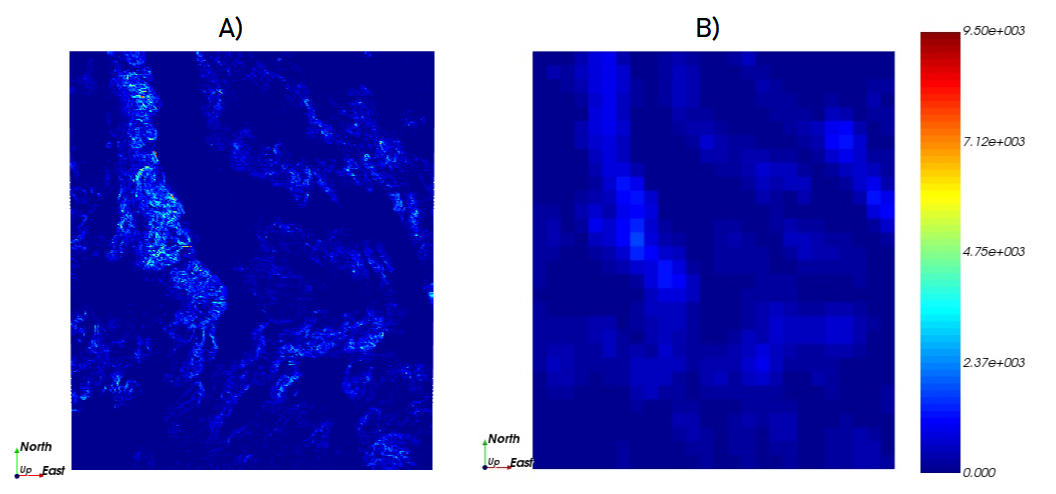
\includegraphics[width=\textwidth]{./Capitulo_1/kriged.png}	
	\caption{Relação do conceito de volume e variância apresentado em imagens. Em A) possuimos o valor exaustivo de um banco de dados, enquanto em B) apresentamos os valores krigados. É possível notar que as estimativas não reproduzem as feições naturais do fenômeno, no entanto, cada bloco estimado é  } 
	\label{volume_var}
\end{figure}
\FloatBarrier



\section{Conclusões} 

Neste capítulo aprendemos um pouco sobre a teoria das variáveis regionalizadas, um conceito determinado na década de 70 pelo professor George Matheron, e que evoluiu ao longo do tempo, facilitando o estudo de variáveis georeferenciadas. Estes conceitos iniciais são abstratos, porém poderosos, pois permitem constituir as bases de hipóteses utilizadas nos modelos geoestatísticos. 


\section{Exercícios}

\begin{exercise}
	Enumere em uma lista todas as variáveis aleatórias regionalizadas que você possui em seu objeto de estudo. Indique ao lado se elas são somáticas ou não. Ex.: Teor-> somático, Condutibilidade hidráulica -> não somático.
\end{exercise}

\begin{exercise}	
 Cinco ações de uma mineradora possuem rentabilidade de 5, 10,20,4 e 5 Unidades monetárias. Se a probabilidade de renda destas ações forem iguais a 40\%, 35\%, 10\%, 10\% e 5\% qual é o valor esperado para a renda de todas as ações. Resp.:8.15 UM
\end{exercise}

\begin{exercise}
	Cinco amostras possuem valor de teor iguais a 2\%, 2.5\%,2.3\%,2.1\% e 2.7\%. Se o volume das amostras é de 5,4,3,5 e 7 $cm^3$ qual é o teor médio das amostras. Resp.: 2,34\%
\end{exercise}
\begin{exercise}	
	\item Prove que o valor do resíduo da função aleatória é ortogonal à sua tendência, ou seja $Cov(R,m) = 0 \forall x \in D$ sendo D o domínio do depósito.
\end{exercise}
\begin{exercise}
	\item Prove que a covariância de duas variáveis aleatórias independentes seja igual a zero. Dica.: Tome o valor de $E(XY) = E(X)E(Y)$
	
\end{exercise}

 
\chapter{Estatística univariada}\label{est_univ}

\begin{myquoting}{Pitigrilli}
	
	Estatística: a ciência que diz que se eu comi um frango e tu não comeste nenhum, teremos comido, em média, meio frango cada um.
\end{myquoting}


\section{Introdução} 

	
As avaliações geoestatísticas geralmente se iniciam com uma avaliação global das amostras. Nesta primeira etapa, o objetivo principal é \textbf{descrever} e \textbf{inferir} informações sobre o comportamento geral das amostras. A chamada \textbf{estatística descritiva} representa o conjunto de técnicas necessárias para resumir informações da realidade observada das amostras, usando formas numéricas ou gráficas para caracterizá-las. Já a chamada estatística inferencial ocupa em tomar inferências da população de dados a partir de informações das amostras. O estudo sistemático das variáveis em termos globais não representam o fenômeno estudado, mas partem do ponto de vista necessário para o início da pesquisa, podendo avaliar inconsistências nos dados e possíveis comportamentos que possam indicar situações favoráveis ou desfavoráveis na análise espacial.


\begin{proposition}
	\textit{Usualmente, os sistemas aos quais estudamos não podem ser isolados em variáveis discretas e independentes. Estes fatores influenciam os primeiros passos da pesquisa, em como e onde coletar espécies ou observações  - \cite{borradaile2013statistics}}
\end{proposition}

A palavra estatística, non entanto, apresenta duplo sentido. Pode representar a \textbf{teoria estatística} ou as medidas realizadas pelos dados. Alguns conceitos iniciais são de extrema importância quando consideramos o uso da estatística clássica univariada 

\begin{definition}[População]
	\textit{conjunto de elementos que tem pelo menos uma característica em comum. No caso da geoestatística a população pode ser considerada analogamente ao conjunto possível de todas as realizações em um domínio geológico considerado}
\end{definition}

\begin{definition}[Amostra]
	\textit{Amostra pode ser considerada como um subconjunto de elementos de uma população. Existem diferentes tipos de amostragens na mineração, como sondagens diamantadas, amostragens de canal, medições de nível freático, etc.}
\end{definition}

Em muitos casos é comum representar este conjunto de dados por tabelas. Sumários que caracterizam as informações de cada subconjunto de amostras no espaço. Muitos softwares de geoestatística e planejamento mineral caracterizam os furos de sondagem a partir de dois ou três arquivos. Geralmente o primeiro arquivo consta uma tabela sobre o posicionamento da boca dos furos na superfície, caracterizando seu posicionamento espacial em um plano cartesiano <x,y,z>. O segundo arquivo geralmente representa a direção dos furos e o comprimento realizado em cada manobra. E um terceiro arquivo geralmente apresenta as propriedades medidas em cada manobra realizada do testemunho.

Uma questão importante a ser considerada nas estatísticas descritivas é sua capacidade de resumo da informação. Estatísticas numéricas são uma alternativa importante para formar concepções que auxiliam na tomada de decisão, mas ao mesmo tempo reduzem a sensibilidade sobre outras questões dos dados. Imagine a figura \ref{Fig1:Cap2}. Temos duas fontes de temperatura equidistantes, uma com $270^{\circ}$ e outra a $-270^{\circ}$. Apesar da diferença abrupta de temperaturas, a temperatura média da parede entre elas é apenas $0^{\circ}$. Um ser humano conseguiria sobreviver facilmente se ocupasse apenas o espaço entre estas duas fontes de temperatura, mas morreria se afastasse delas. 

\FloatBarrier
\begin{figure}[!htb]
	\centering
	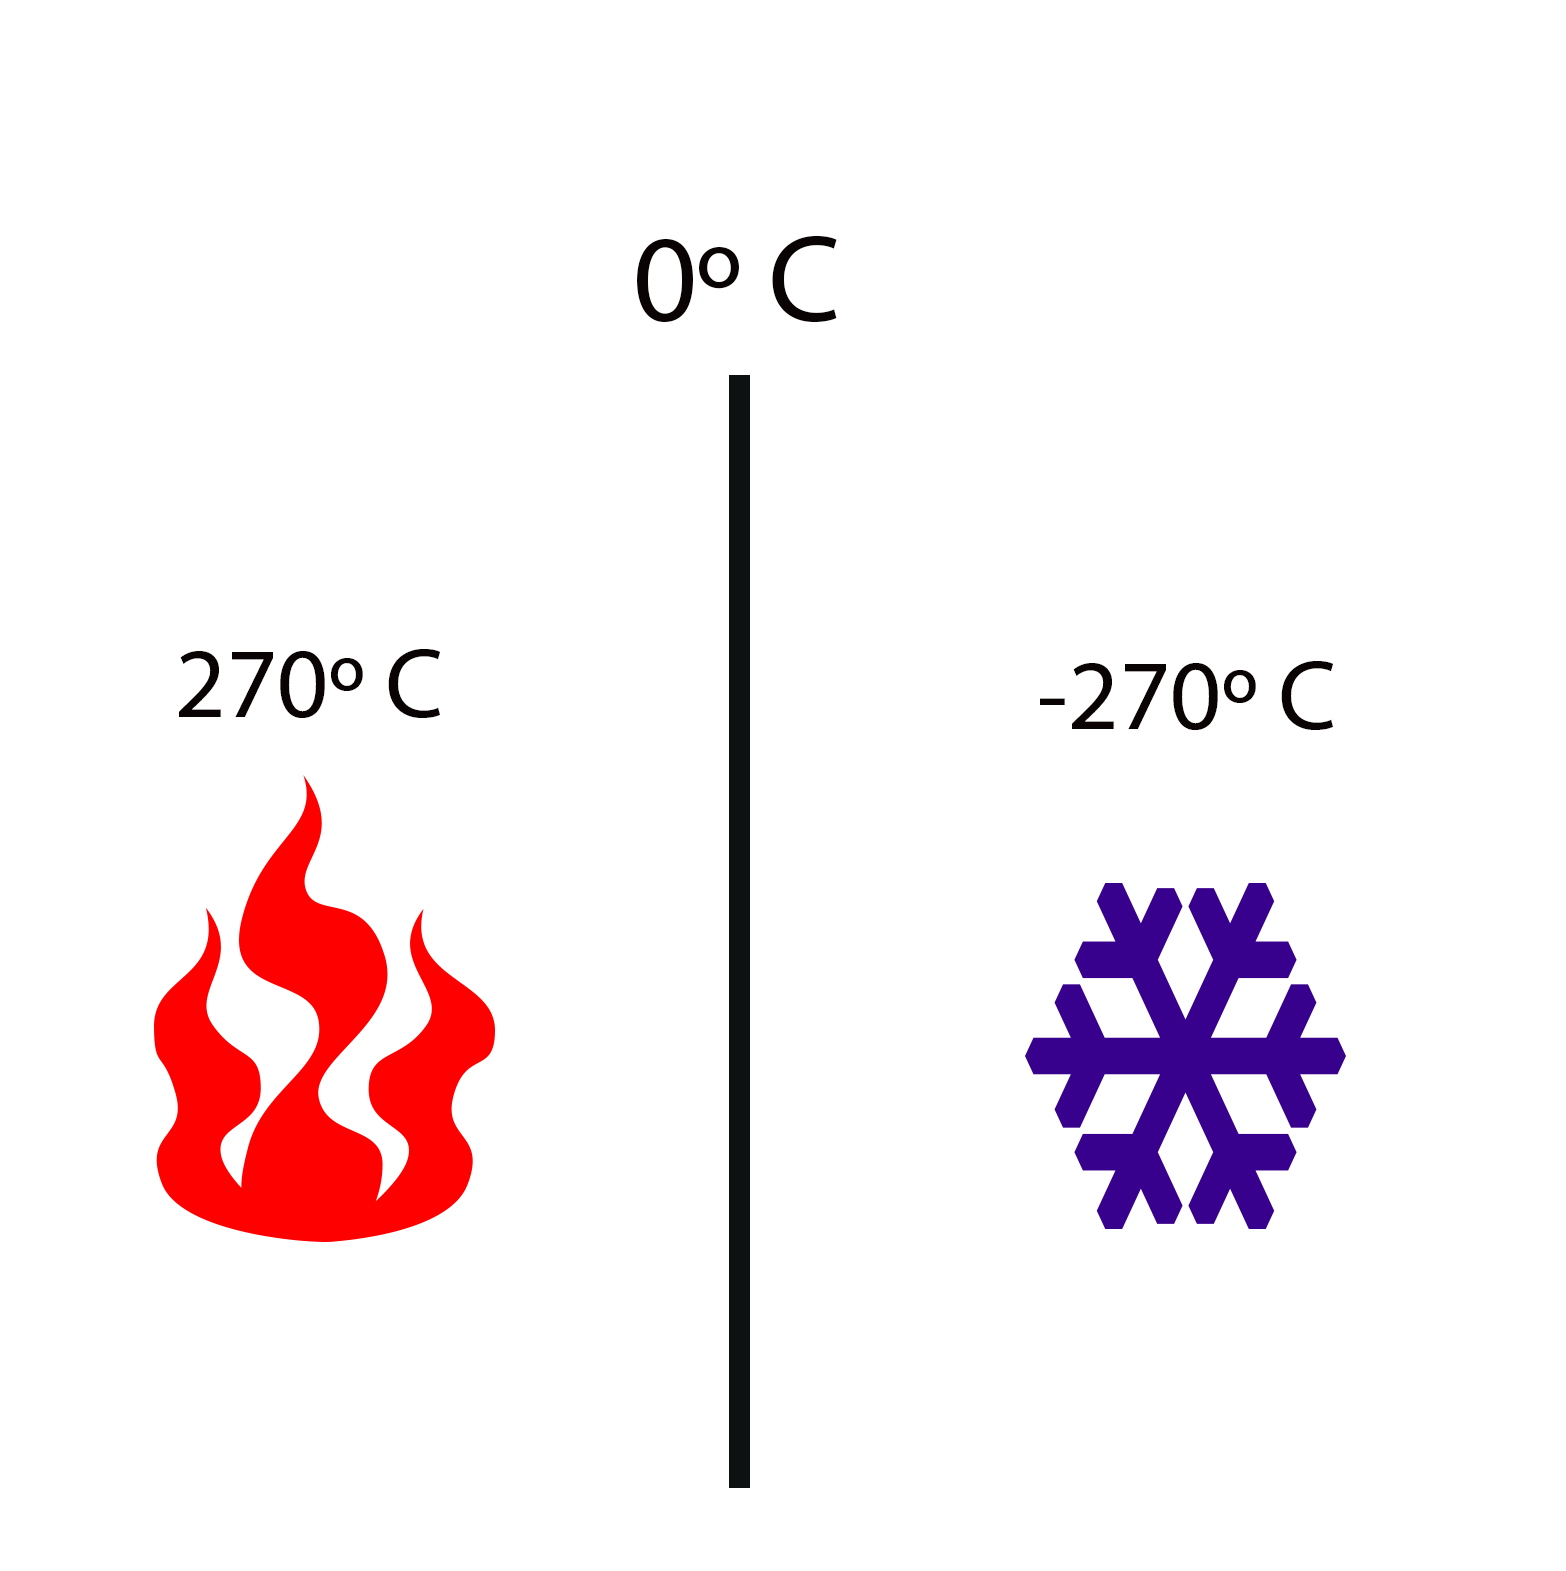
\includegraphics[scale=0.5]{./Capitulo_2/Figura_1_Fire_Ice.png}	
	\caption{Duas fontes de temperatura equidistantes, uma quente e outra fria. A temperatura média da parede que separa estas fontes é igual a média das temperaturas, o que não representa toda a complexidade do fenômeno.}
	\label{Fig1:Cap2}
\end{figure}
\FloatBarrier

Apesar da média ser uma medida muito útil para ser utilizada na descrição dos dados, utilizada sozinha pode gerar interpretações erradas sobre o problema. Convenciona-se que o uso de estatísticas descritivas deve ser múltiplo, optando por utilizar não apenas uma, mas diferentes técnicas de avaliação. 

O uso de estatísticas descritivas permite em muitos casos 

\begin{enumerate}
	\item Avaliar se as proporções globais possam estar acima do cut-off esperado
	\item Identificar a facilidade da aplicação dos métodos clássicos de acordo com as distribuições de frequência
	\item Auxiliar no dimensionamento de malhas de sondagem principalmente nas etapas iniciais (\textit{greenfield}) na mineração
	\item Identificar a possibilidade da divisão de domínios se apresentadas frequências multimodais 
\end{enumerate}

\begin{proposition}
	\textit{Estatísticas univariadas são a primeira alternativa para analisar dados. Quando as amostras ainda são escassas, principalmente nas fases iniciais da pesquisa mineral, estas ferramentas são extremamente úteis para avaliarem de forma genérica os resultados das campanhas. Se bons resultados podem ser gerados a partir de estatísticas univariadas, a confiança no projeto aumenta suas perspectivas, no entanto, se os dados demonstrarem condições pobre das estatísticas, ainda podemos apostar em uma melhor avaliação do depósito}
\end{proposition}

É importante salientar que informações a partir de estimativa e interpolação não podem gerar dados além dos limites estipulados pela estatística descritiva univariada. Qualquer método de inferência não extrapola os valores mínimos e máximos de um depósito mineral. Descrever é antes de tudo um passo que necessita encontrar propriedades de algo. A descrição deve conter os aspectos mais importantes de um depósito mineral, tal como mínimo e máximo encontrados, valores médios, dispersão. Da mesma forma que desenhar é uma atividade altamente explicativa para descrever um problema, as estatísticas gráficas desempenham papel fundamental na avaliação inicial.


%%%%%%%%%%%%%%%%%%%%%%%%%%% ESTATÍSTICAS PONTUAIS %%%%%%%%%%%%%%%%%%%%%%%%%%%

\section{Estatísticas pontuais}

Como dito anteriormente, o conceito estatística pode ser dúbio, ao mesmo tempo que enfoca na 'teoria estatística' ou em \textbf{funções aplicadas em dados}. Quando estas funções forem aplicadas em todos os dados de um universo são chamadas de \textbf{parâmetros}. Qualquer função realizada a partir de dados pode ser considerada uma estatística, ou um \textbf{estimador}, no entanto, algumas delas são mais usuais, por conseguirem a partir de dados aproximar as estatísticas de seus respectivos parâmetros.

Outra forma de resumir e descrever os dados é através de estatísticas pontuais. Elas resumem a informação do conjunto de amostras em uma única medida descrevendo-o como um todo.

\begin{definition}[Estatísticas pontuais]
\textit{Estatísticas pontuais são funções realizadas a partir dos dados para calcular valores que representam propriedades do conjunto. Dentre as categorias mais conhecidas possuímos medidas de \textbf{centralidade}, \textbf{dispersão}, \textbf{asssimteria}, \textbf{achatamento} }
\end{definition}

Se fôssemos comparar a descrição pontual com o retrato falado de um criminoso, cada estatística seria apenas uma parte do rosto, a média o nariz e a variância as orelhas, por exemplo. Uma das ferramentas utilizadas para entender estas estatísticas visualmente também é conhecida como faces de Chernoff, como demonstrado na figura \ref{Fig_chernoff}

\FloatBarrier
\begin{figure}[!htb]
\centering
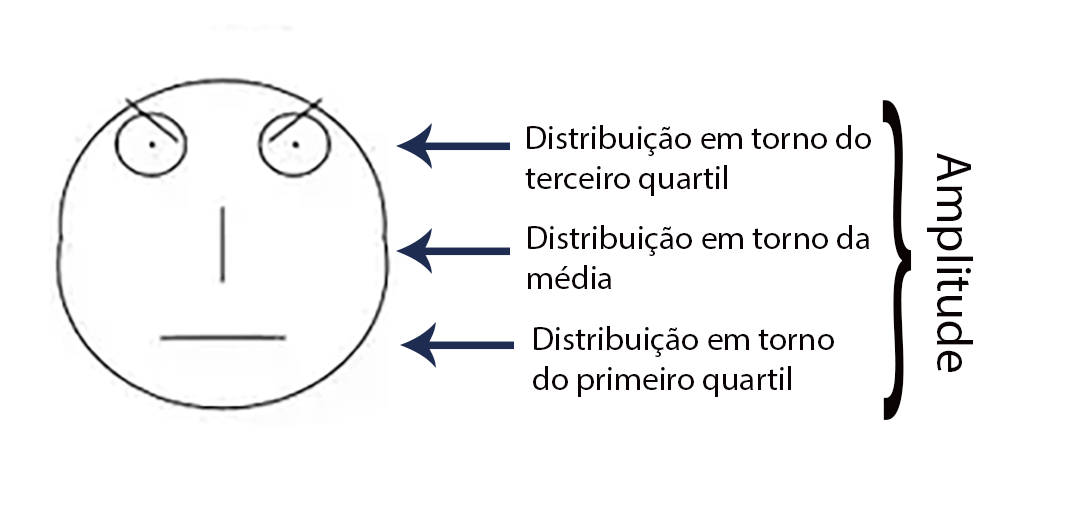
\includegraphics[scale=0.98]{./Capitulo_2/faces.png}	
\caption{Exemplo das faces de Chernoff e as características das estatísticas com estruturas da face.}
\label{Fig_chernoff}
\end{figure}
\FloatBarrier

\FloatBarrier
\begin{figure}[!htb]
	\centering
	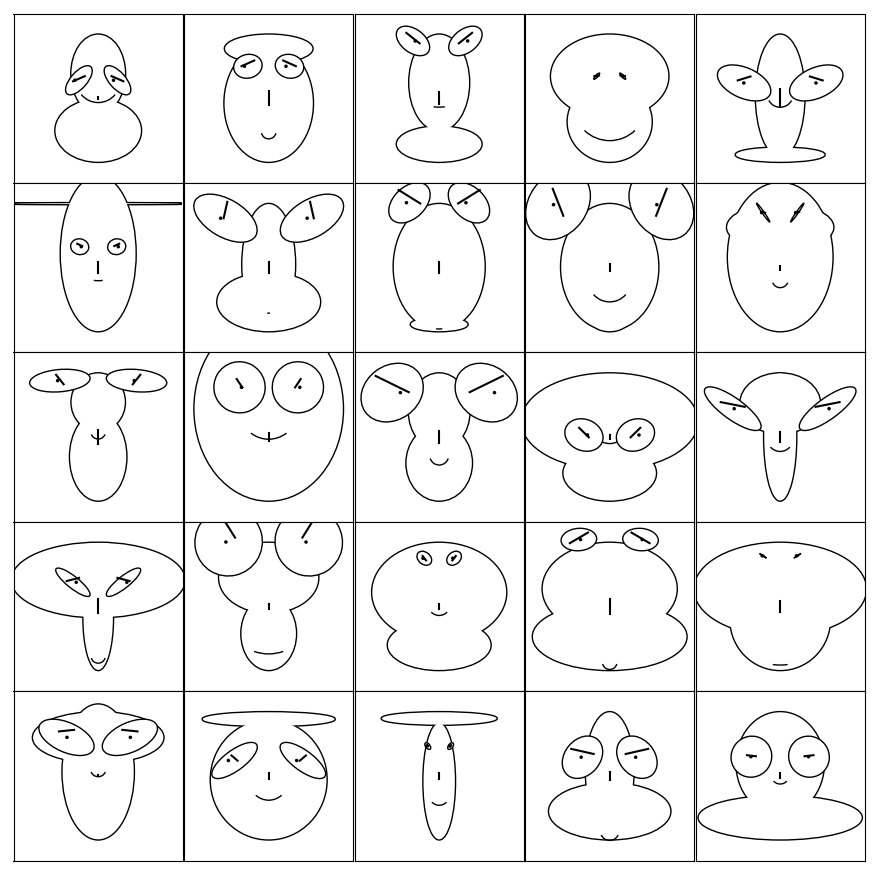
\includegraphics[scale=0.5]{./Capitulo_2/predicted.png}	
	\caption{Diferentes faces de Chernoff para diferentes variáveis}
	\label{Fig_chernoff_2}
\end{figure}
\FloatBarrier

\begin{proposition}
\textit{Faces de Chernoff foram criadas por Herman Chernoff em 1973, como uma forma de representar dados multivariados de forma a ser discernido facilmente por um observador humano. As faces constituem em linhas desenhadas em duas dimensões que contém uma série de estruturas faciais.} - \cite{morris2000experimental}
\end{proposition}


É importante salientar que apenas uma estatística pontual não é uma medida que garante informação completa a respeito de um conjunto de dados. Um depósito mineral pode ter valor médio de 50g de ouro por tonelada, enquanto outro tenha 45g de ouro por tonelada, e ainda assim o segundo depósito seja mais rico, pois a análise deve ser realizada sobre as proporções gerais dos dados. Isso acontece porque as medidas pontuais de tendência central como a média devem estar sempre associadas com uma medida de dispersão. Se o depósito de 50 g por tonelada possuir uma menor dispersão, e o depósito de 45 g/ton possuir uma maior, para um dado cut-off o depósito de 45g/ton pode ser mais rico.

A Figura \eqref{explicacao} demonstra esta situação graficamente. Notamos que a a distribuição A, apesar de possuir uma média menor que a distribuição B, ainda assim relata um depósito mais rico para o cut-off considerado. 

\FloatBarrier
\begin{figure}[!htb]
\centering
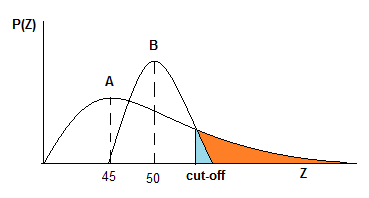
\includegraphics[scale=1]{./Capitulo_2/explicacao1.png}	
\caption{Exemplo de duas distribuições A e B relatando um depósito mais rico A com média menor que B. Área azul mostrando a contribuição da distribuição B acima do cut-off e área laranja mostrando a contribuição de A acima do cut-off}
\label{explicacao}
\end{figure}
\FloatBarrier

\subsection{Medidas de tendência central} 

As medidas de tendência central são estatísticas calculadas a partir das amostras que representam o centro de massa do conjunto. Analogamente ao ponto de equilíbrio de uma barra, estas representam o centro de dispersão dos dados. 
Note que esta é uma convenção matemática. O valor médio não representa necessariamente um valor do conjunto de amostras e nem tão pouco pode representar um valor mais provável, mas apenas um centro da dispersão dos dados.

\begin{proposition}
\textit{Se lançarmos um dado de seis lados centenas de vezes, e anotarmos o valor realizado em cada jogada, teremos uma tabela com cada número e sua possível frequência. É esperado que a média deste conjunto de dados seja $~3.5$, pois a frequência entre os números obtidos nos lançamentos será aproximadamente parecida $(6+1)/2$. Este valor apesar não é real, pois não podemos obter metades de uma face de um dado, mas representa o centro de dispersão destes valores.}  
\end{proposition}


As medidas de tendência central mais comuns são a média aritimética, a moda, a média ponderada e a mediana. 

\subsubsection{Média aritmética} 

A média aritimética pode ser descrita segundo a equação \eqref{eq3:media aritmetica} em que x são os valores das amostras e n o número de amostras. Se a média aritmética for calculada a partir de uma população finita de todos os seus elementos a média $\bar{x}$ é equivalente ao valor esperado da variável $\mu=E(X)$. 

\begin{equation}\label{eq3:media aritmetica}
\bar{x} = \frac{1}{n}\sum_{i = 0}^{n} x_i
\end{equation}

Muitas vezes é necessário calcular a média aritmética de um agrupamento de dados a partir de um histograma, por exemplo. Neste caso podemos calcular a média aritmética como 

\begin{equation}\label{eq3:media aritmetica}
\bar{x} = \frac{1}{n}(f_{1}c_{1} + f_{2}c_{2} + ...+ f_{n}c_{n} ) = \frac{1}{n}\sum_{i = 0}^{n} f_{i}c_{i}
\end{equation}

Em que $f_{i}$ é a frequência de cada classe $c_{i}$.

\subsubsection{Moda}

Para variáveis inteiras, a informação mais importante é a frequência de cada valor da variável. Neste caso uma das informações importantes de tendência central é a moda, como o valor com maior frequência nos dados. No caso de variáveis reais contínuas, frequências são desprovidas de significado, sendo impossível calcular seus valor nas amostras, apenas por classes.

\begin{definition}[Moda]
\textit{A moda $M_{0}$ de uma amostra é a observação com maior frequência nos dados} 
\end{definition}

A moda nem sempre é um valor fixo, pois diferentes valores ou classes podem possuir mesma frequência. Quando um histograma apresenta dois picos, este também é chamado de \textbf{bimodal}. Quando apenas um é apresentado, chamamos o histograma de \textbf{unimodal}

\subsubsection{Média ponderada}

A média ponderada considera que cada valor pode possuir uma importância diferenciada, e a ele é associado um valor chamado \textbf{peso}. A equação \eqref{eq4: media ponderada} demonstra o valor de uma média ponderada

\begin{equation}\label{eq4: media ponderada}
\bar{x} =  \frac{\sum_{i = 0}^{n} p_{i} x_{i}} {\sum_{i = 0}^{n} p_{i}}
\end{equation}

Em que $p_{i}$ corresponde o peso de cada um dos valores para as $n$ variáveis possíveis. A relação de cada peso pela soma total destes pesos também é chamado de ponderador e pode ser representado pela equação \eqref{pesos}

\begin{equation}\label{pesos}
\lambda_i = \frac{p_i}{\sum_{i=1}^{n}p_i} \forall i 
\end{equation}

A média ponderada pode ser reescrita em termos de seus ponderadores de acordo com a equação \eqref{eq4: media ponderada_pes}

\begin{equation}\label{eq4: media ponderada_pes}
\bar{x} =  \sum_{i = 0}^{n} \lambda_{i} x_{i} 
\end{equation}

\subsubsection{Mediana} 

A mediana é uma representação do valor associado a aproximadamente 50\% da frequência total dos dados. 

\begin{definition}[Mediana]
\textit{Se o número de elementos (n) for ímpar, a mediana é igual a $\frac{n+1}{2}$ elemento. Se o número de elementos for par, então a mediana é igual a média do $\frac{n}{2}$ elemento e o $\frac{n}{2}+1$ elemento} 
\end{definition}

\begin{proposition}
\textit{Suponha que a amostra consiste em 10 observações: 6,3,4,7,4,6,7,6,5,3, nós teremos um número de elementos n= 10, sendo este valor par. Ordenando o conjunto de dados teremeos 3,3,4,4,5,6,6,6,7,7. Então a mediana é igual a média entre o $5^{\circ}$ e o $6^{\circ}$ elemento, correspondendo ao valor de $(5+6)/2=5,5$.}
\end{proposition}

\subsection{Medidas de posição}

As medidas de posição são aquelas tomadas em relação a outras, ou seja em seu contexto geral com outros valores. Entre elas as mais comuns são os \textbf{percentis}, \textbf{quartis}, e \textbf{decis} 

\subsubsection{Percentis ou quantil} 

Uma das formas de se avaliar a posição dos dados é quanto a sua frequência. Um percentil ou quantil representa o valor correspondente a uma proporção total dos dados.

\begin{definition}[Percentil ou quantil]
\textit{Um percentil ou quantil $c_{p}$ de uma amostra corresponde ao valor imediatamente superior ou igual a $100xp\%$ e imediatamente inferior a $100x(1-p\%)$ dos dados} 
\end{definition}

\begin{proposition}
\textit{Suponha que a amostra a seguinte amostra: $\{6,3,4,7,4,6,7,6,5,3,4,2\}$ nós teremos um número de elementos n= 10. Ordenando o conjunto de dados teremos $\{2,3,3,4,4,4,5,6,6,6,7,7\}$. logo as proporções dos dados serão $\{2:8\% , 3:17\%, 4:25\%, 5:8\%, 6:25\%, 7:17\%\}$. As proporções acumuladas serão equivalentes a $\{2:8\% , 3:25\%, 4:50\%, 5:58\%, 6:83\%, 7:100\%\}$. Então o percentil de 67\% será o valor imediatamente superior a 58\% e inferior a 83\%. Utilizando uma interpolação linear temos que $(67\%-58\%) * (6-5)/(83\%-58\%) + 5 =5.36$ .}
\end{proposition}

\subsubsection{Quartis} 

O \textbf{quartil} são medidas de posição que correspondem a 4 posicionamentos especiais dentro do conjunto de dados. O primeiro quartil representa o \textbf{o percentil de 25\%}, o segundo quartil representa \textbf{o percentil de 50\% ou a mediana}, e o terceiro quartil representa \textbf{o percentil de 75\% dos dados}. 

\begin{proposition}. 
\textit{Se obtivermos um conjunto de dados iguais a ${50,34,27,54,25,43,15,12}$ contendo 8 valores então podemos ordená-los em crescente de tal forma que teremos ${12,15,25,27,34,43,50,54}$. O valor do primeiro quartil será, segundo os dados ordenados, 15. O terceiro quartil será 43. E a mediana será igual a 27.}
\end{proposition} 

\subsection{Medidas de dispersão}

Outras medidas importantes são as de dispersão. Entre as mais comuns podemos citar a \textbf{variância}, o \textbf{desvio padrão} e a \textbf{amplitude} dos dados. 

\subsubsection{Amplitude} 

A forma mais simples de se medir a dispersão dos dados é considerar sua amplitude. A maior vantagem em se definir a amplitude é sua simplicidade de cálculo, porém esta estatística é muito afetada por valores extremos

\begin{definition}[Amplitude]
\textit{Corresponde a diferença do valor máximo obtido nos dados $x_{max}$ com o valor mínimo $x_{min}$.} 
\end{definition}

\subsubsection{Invervalo Interquartil} 

Uma forma de se avaliar uma medida de dispersão menos afetada pelos valores extremos é o intervalo interquartil

\begin{definition}[Intervalo interquartil]
\textit{Corresponde a diferença do valor do terceiro quartil ($Q_{75}$) com o valor do primeiro quartil ($Q_{25}$).} 
\end{definition}

\subsubsection{Variância} 

A variância pode ser descrita pela equação \eqref{eq5:variancia}

\begin{equation}\label{eq5:variancia}
s^2 = \frac{\sum_{i = 0}^{n} \left( x_i - \bar{x} \right)^2}{n-1}
\end{equation}

Em que $n-1$ é o número de graus de liberdade da amostra, tal que este pode ser definido pelo número de amostras menos o número de estatísticas utilizadas durante o cálculo. Note que para a operação da variância precisamos antes determinar o valor da média. É uma medida que não apresenta as mesmas unidades que a das amostras, para isso geralmente utilizamos o desvio padrão, que pode ser calculado como a raiz quadrada dos valores da variância $(s=\sqrt{s^{2}})$. 

Em alguns casos também é possível calcular a variância para classes e não para valores, assim como a média aritmética. Neste caso podemos calcular a variância a partir de 

\begin{equation}\label{eq5:variancia}
s^2 = \frac{\sum_{i = 0}^{n} f_{i}\left( c_i - \bar{c} \right)^2}{n-1}
\end{equation}

Em que $c$ corresponde ao valor da classe e $f_{i}$ o valor da frequência associada aquela classe.



\subsection{Assimetria}

Outra medida pontual importante também é a assimetria. Esta se caracteriza pela diferença de proporções de uma distribuição de amostras segundo ao redor de seu valor mais frequente. 

A figura \eqref{Fig10_1} demonstra a distribuição de dados assimétrica. O item a) representa uma distribuição assimétrica positiva, enquanto o item b) representa uma distribuição assimétrica negativa. A assimetria positiva é caracterizada por um valor da mediana abaixo do valor médio, enquanto a assimetria negativa se caracteriza por uma alta proporção de valores altos. 


\begin{figure}[H]
\centering
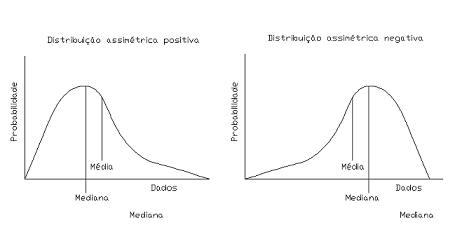
\includegraphics[scale=1.0]{./Capitulo_2/figura10_1.png}	
\caption{Assimetria de uma distribuição de dados a) Assimetria positiva b) assimetria negativa }
\label{Fig10_1}
\end{figure}

Uma das medidas de assimetria mais comuns é o coeficiente de Pearson que pode ser expresso pela equação \eqref{eq5:coeficiente de pearson}

\subsubsection{Coeficiente de assimetria de Pearson}

\begin{equation}\label{eq5:coeficiente de pearson}
S_{p}= 3\left( \bar{x} - M_e\right)/s
\end{equation}

Em que $M_e$ é a moda dos dados, $\bar{x}$ é o valor médio das amostras e s é o desvio padrão das amostras. 

\begin{proposition}
\textit{Imagine uma variável com valor de média $\bar{x} = 198.89$, valor de mediana $M_e = 128.15$ e valor de desvio padrão igual a $s = 180.56$. O valor do coeficiente de assimetria será igual a $3(192.89 - 128.30)/180.56 = 1.07$, demonstrando assimetria nos dados.}
\end{proposition}

Distribuições com característica de assimetria positiva são muito comuns na avaliação de depósitos minerais, principalmente no tratamento de commodites erráticos tal como ouro e diamante. Nesses depósitos podem ocorrer anomalias raras e uma amostra constituir em alto valor. Esta propriedade também é chamada de efeito pepita e será melhor tratada no capítulo de Continuidade espacial. 


\subsection{Coeficiente de variação}

Em certos momentos é importante comparar variáveis aleatórias de tipos diferentes. Para sabermos se uma distribuição é mais errática que outra, neste caso, não bastaríamos comparar seus valores de variância. Valores que possuam médias maiores tendem a apresentar dispersões também maiores. Para isso utilizamos o coeficiente de variação, que nada mais é do que o desvio padrão de uma distribuição pelo seu valor médio. Desta forma "igualamos" diferentes distribuições em um único coeficiente comparativo. 

O coeficiente de variação pode ser dado pela equação \eqref{eq5:coeficiente de var}

\begin{equation}\label{eq5:coeficiente de var}
CV = \frac{s}{\bar{x}}
\end{equation}

Os coeficientes de variação são medidas importantes para a pesquisa mineral, porque são a primeira forma utilizada para classificar depósitos minerais segundo sua regularidade. O livro de \citep{maranhao1985introduccao} demonstra a classificação de depósitos minerais de acordo com o coeficiente de variação, tal como na tabela \ref{Tabela:regularidade}.

\FloatBarrier
\begin{table}[!htb]
	\centering
	\caption{Regularidade dos depósitos minerais de acordo com a classificação do coeficiente de variação}
	\vspace{0.5cm}
	\label{Tabela:regularidade}
	\resizebox{\textwidth}{!}{
	\begin{tabular}{lll}
		\toprule
		Regularidade & Coeficiente de variação & Exemplo \\
		\midrule
		\midrule
		Regulares&5\% <CV< 40\%& Jazidas de ferro, manganês, níquel, cobalto \\
		Irregulares&40\%<CV<100\%& Jazidas de fluorita, barita, grafita, coríndon \\
		Muito irregulares&100\%<CV<150\%& Jazidas de tungstênio em tactitos, ouro \\
		Extremamente irregulares&CV>150\%& Pegmatitos com berilo, tantalita, columbita \\
		\bottomrule
	\end{tabular}%
	}
\end{table}
\FloatBarrier

Valores de coeficiente de variacão maiores representam geralmente um maior desafio para a aplicação de técnicas de geoestatística, pois geralmente apresentam alta variabilidade ou erraticidade dos dados.

\subsection{Conjugando estatísticas pontuais}

Como dito anteriormente, é sempre importante conjugar estatísticas pontuais diferentes de forma a garantir a melhor informação possível. Uma destas alternativas é adicionar ao valor médio um número de desvios padrões de forma a garantir que um conjunto de dados esteja situado dentro destes limites $(\bar{x}) \pm k s)$. Para isso utilizaremos uma das mais renomadas relações estatísticas.
	
	A desigualdade de Chebyshev é uma identidade que implica em um valor mínimo de probabilidade para que uma realização esteja dentro de um intervalo múltiplo do desvio padrão. Podemos definir a equação \eqref{eq6:Chebyshev} como a desigualdade de Chebyshev.
	
	\begin{equation}\label{eq6:Chebyshev}
	P\left(|X-\mu| \geq k\sigma\right)\leq1/k^2
	\end{equation}
	
	Em que $X$ é o valor da variável aleatória, $\mu$ é o valor da média da população, $\sigma$ é o valor do desvio padrão da população e k é uma constante proporcional. A desigualdade de Chebyshev é independente do valor da distribuição de probabilidades para a variável aleatória. Apesar de não possuirmos os valores $(\mu, \sigma)$ correspondentes aos parâmetros da população, podemos estimar os valores a partir das estatísticas das amostras. Se o número de amostras for grande o suficiente e as técnicas de amostragem bem selecionadas,  podemos dizer que $(\mu \sim \bar{x}, \sigma \sim s)$ 

Para um k igual a 2, sabemos que existe uma probabilidade de no mínimo 75 por cento de que o valor da amostra esteja em dois desvios padrões da média. Podemos caracterizar as amostras então por uma medida de posição e de dispersão conjuntamente. Ao descrever as amostras é bem claro que devemos associar no mínimo dois de seus parâmetros, como por exemplo, dizer que as amostras de teor de ouro possuem valores entre $\left(50 \pm 20 \right) ppm$ em que 20 representaria dois desvios padrões de 10 ppm e 50 ppm seu valor médio.
		


\section{Validação do banco de dados e valores outliers}

A primeira etapa da geoestatística é a validação das amostras. Devemos antes de tudo verificá-las para que não encontremos valores discrepantes (outliers) ou incoerências nos dados. Análises realizadas com valores muito discrepantes pode acabar gerando resultados espúrios e inconsistentes com a realidade. 

\begin{definition}[Outlier]
	\textit{Um outlier é considerado um valor ou observação caracterizado pela sua relação entre o restante de observações que fazem parte das amostras. O seu distanciamento em relação as observações é essencial para fazer sua caracterização. Estas observações também são chamadas de 'anormais', contaminantes, estranhas, extremas ou aberrantes} - \cite{figueira1998identificaccao}
\end{definition}

 É importante entender que os dados anômalos nem sempre são valores errados. Eles podem ser valores reais representantes de uma anomalia da natureza. Poderíamos encontrar, por exemplo, em um depósito de ouro uma pepita com um valor agregado muito alto, mas apesar de ser um dado correto ele não representa o conjunto de amostras como um todo. \citet{machado2012alternativa} indica que o surgimento de valores anômalos podem ocorrer por diversas formas, entre elas: 

\begin{enumerate}
	\item \textbf{Valores errôneos:} As possíveis causas são os erros de análise ou de digitação, troca de amostras, contaminações de amostras ou até mesmo fraude. 
	\item \textbf{Valores pertencentes a outra população:} Podem ocorrer devido à mistura de diferentes teores ou litologias, ou que possuem processo formacional em tempos geológicos distintos. A revisão dos domínios geológicos, neste caso é recomendado, de forma a tratar e estimar os dados separadamente. 
	\item \textbf{Valores pertencentes a mesma população:} Podem ocorrer eventos metalogenéticos que favoreçam a concentração de uma propriedade em parte do depósito. Estes eventos estão relacionados também ao chamado \textbf{efeito pepita}, em que proporções erráticas podem aparecer apenas em locais distintos do depósito, em regiões pequenas. 
\end{enumerate}

 A Tabela \ref{Tabela1:Minerio_de_ferro} é um exemplo de como valores anômalos podem aparecer. Nota-se claramente que as amostras 1 e 3 estão erradas. Primeiramente porque não existem valores de teor percentuais acima de 100$\%$ e também porque não existem teores descritos como letras. No entanto, a amostra 4 também está errada, porque o minério composto por limonita não pode apresentar um valor de teor de ferro de 72$\%$, pois é incompatível com a  química da mineralogia. 

\FloatBarrier
\begin{table}[!htb]
\centering
\caption{Tabela de teores do minerio de ferro}
\vspace{0.5cm}
\label{Tabela1:Minerio_de_ferro}
\begin{tabular}{r|lr}
	Índice & Minério & Teor($\%$) \\ 
	\hline                               
	1 & Hematita compacta       & 120$\%$ \\
	2 & Hematita granular       & 53$\%$ \\
	3 & Magnetito               & 0.i3 \\
	4 & Limonita                & 72$\%$ \\
\end{tabular}
\end{table}
\FloatBarrier

\begin{proposition}
	\textit{Pode até mesmo parecer um clichê, mas a melhor forma de se analisar outliers é com bom senso. Devemos entender o problema, analisá-lo profundamente na hora de limparmos o banco de dados. Permitir que bancos de dados sejam transmitidos antes de uma boa verificação pode resultar no fracasso de uma análise destes dados.}
\end{proposition}

Diversas são as formas de identificação de valores outliers. Técnicas para valores em apenas uma variável são muito conhecidas, no entanto, deve-se entender que um valor anômalo depende de sua dimensão analisada. Uma amostra outlier considerando variáveis distintas pode não ser um valor um valor anômalo quando considerado um problema multivariado. 

Uma das ferramentas mais comuns para identificação de valores anômalos é o gráfico boxplot. Ele demonstra a disposição dos dados em um eixo e limita os valores das amostras em uma caixa contendo os quartis das amostras. Os valores que se situam acima ou abaixo das retas formadas pela adição e subtração 1,5 vezes o intervalo interquartil dos valores máximo e míno dos dados representam outliers. O intervalo interquartil é também determinado como a diferença entre os valores do terceiro quartil e do primeiro quartil. A figura \ref{fig7_1} demonstra o gráfico boxplot e suas dimensões. 

\FloatBarrier
\begin{figure}[!htb]
\centering
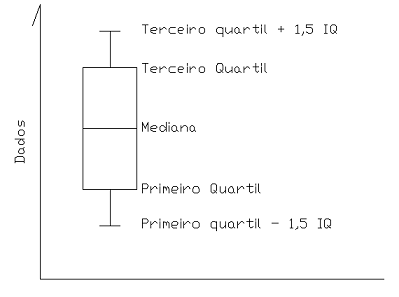
\includegraphics[scale=0.60]{./Capitulo_2/figura7_1.png}	
\caption{Representação de um gráfico de caixa dividida entre os intervalos das amostras }
\label{fig7_1}
\end{figure}
\FloatBarrier


Os valores anômalos ou outliers são demonstrados na figura \ref{Fig8_1} como pontos circulados fora das barras que representam os limites de aceitação dos valores da amostra.

\FloatBarrier
\begin{figure}[!htb]
	\centering
	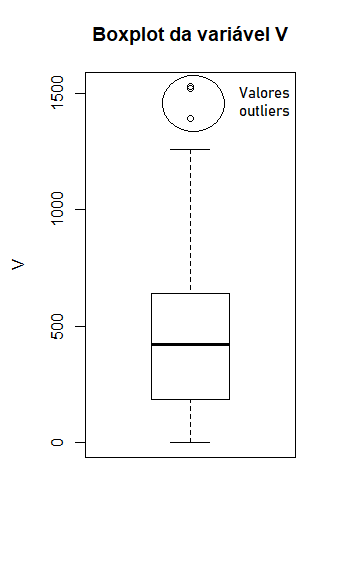
\includegraphics[scale=0.60]{./Capitulo_2/figura8_1.png}	
	\caption{Representação dos valores outliers no gráfico boxplot - Pontos circulados em vermelho }
	\label{Fig8_1}
\end{figure}
\FloatBarrier

Muito cuidado deve ser utilizado com esta ferramenta. Em alguns casos distribuições de dados assimétricas podem gerar no gráfico boxplot uma quantidade de valores anômalos absurdas. A melhor forma de lidar com valores outliers é o bom senso, ferramentas são úteis, mas não devem ser o critério determinante na maioria dos casos.

\FloatBarrier
\begin{figure}[!htb]
	\centering
	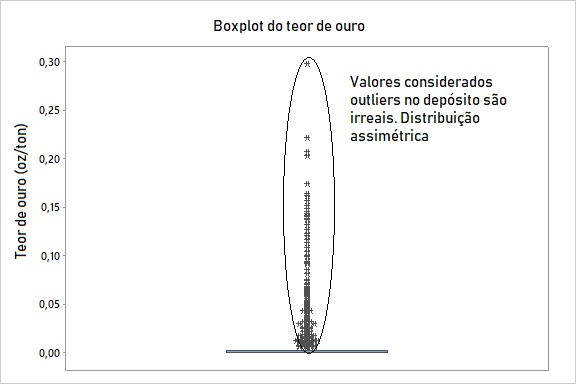
\includegraphics[scale=0.95]{./Capitulo_2/Boxplot_Au.jpg}	
	\caption{Valores outliers em uma distribuição assimétrica dos dados. Nota-se que grande parte da informação é considerada outliers. Neste caso é necessário bom senso para não se remover informações desnecessárias e prejudicar a análise de dados. }
	\label{Fig8_1}
\end{figure}
\FloatBarrier

Após a identificação de valores anômalos é possível realizar o tratamento destes dados. É imprescindível entender que bancos de dados \textbf{nunca} devem ser alterados, apenas estatísticas. A alteração ou remoção de dados é considerada uma atitude imoral para analistas de dados. 

\begin{remark}
	É importante entender que um banco de dados \textbf{nunca} deve ser alterado. Apenas as estatísticas são cabíveis a manutenção. A alteração de dados reais pode ser considerada um ato imoral, principalmente na mineração, onde o trabalho, segurança e condições de vidas de muitas pessoas estão em jogo. 
\end{remark}

Diversas alternativas podem ser utilizadas para o tratamento de valores outliers. Dentre elas podemos citar 

\begin{enumerate}
	\item \textbf{Truncamento:} Após identificar valores outliers é possível normalizar seus valores para os valores extremos (máximo ou mínimo), ao desconsiderá-los. O truncamento de dados na geoestatística deve ser feito de forma a evitar que os valores anômalos não alterem significativamente as estatísticas globais. Como regra de ouro considera-se que o truncamento deve ser feito sem que se altere mais do que 10\% dos valor médio das amostras.
	\item \textbf{Remoção:} Em alguns casos a remoção dos valores outliers pode ser feita. Se a proporção de dados removidos for alta, é possível alterar excessivamente as estatísticas, por isso muito cuidado deve ser feito ao considerar uma amostra como outlier.
	\item \textbf{Reescalonamento}: Dependendo da distância relativa dos outliers com o contexto geral das amostras é possível realizar uma redução de suas distâncias até o valor máximo desconsiderando-os. 
	
\end{enumerate}

\section{ Descrição espacial das amostras}

A geoestatística é uma ciência que prevê a utilização de informações no espaço, e para isso muitas vezes utilizamos informações de mapas. Mapas são representações visuais de uma região que são dotados de informações como \textbf{escala}, \textbf{legenda}, \textbf{título}, \textbf{orientação}. 

 Mapas de localização destas amostras são uma ferramenta gráfica muito importante para determinar o comportamento de variáveis no espaço. Mapas devem ser feitos de forma cuidadosa, representando escalas condizentes com o objeto de estudo e garantindo a melhor visualização possível das amostras.

\begin{remark}
	\textit{A qualidade desejada de um mapa varia de acordo com a investigação. Tipicamente a reprsentação de um mapa deve ser limpa, sem valores altos ou baixos umbíguos, e mostrar os dados o menos distorcidos possível com um mínimo de artefatos computacionais} - \cite{gustavsson1997visualization}
\end{remark}

 Estas informações nos permitem identificar regiões consideradas mais ricas, regiões onde ocorrem agrupamentos característicos dos dados, e o layout das malhas de amostragem. A figura \ref{Fig1_1} demonstra um depósito polimetálico de Jura. O atributo é o tipo de rocha de um dado período geológico.  

\FloatBarrier
\begin{figure}[!htb]
\centering
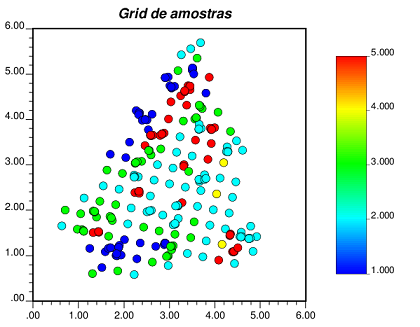
\includegraphics[scale=1]{./Capitulo_2/figura1_1.png}	
\caption{Disposição das amostras no espaço. Cores diferenciadas mostrando tipos de rocha em períodos geológicos diferentes}
\label{Fig1_1}
\end{figure}
\FloatBarrier

Podemos ver que as amostras estão dispostas de forma irregular em um formato de delta de um rio. A orientação do tipo de rocha 1 se encontra ao oeste e parte ao sul, enquanto a do tipo 5 se encontra distribuído mais ao norte. Qualquer estimativa realizada a partir desta configuração de amostras deve respeitar os valores iniciais. Se por exemplo, iniciássemos uma explotação cujo o interesse seria o litotipo 1, provalvelmente começaríamos a retirar o material de oeste para leste para reduzir o fluxo de caixa do empreendimento. 

A \ref{Fig2_1} demonstra a propriedade de teor de Cádmio obtida nestas amostras no depósito. Podemos verificar sua distribuição segundo esta disposição deltaica. 

\FloatBarrier
\begin{figure}[!htb]
\centering
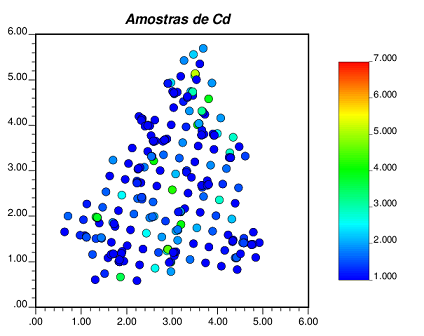
\includegraphics[scale=1]{./Capitulo_2/figura2_1.png}	
\caption{Disposição do Cd}
\label{Fig2_1}
\end{figure}
\FloatBarrier

As informações disponíveis nestes mapas nos permite associar as informações entre as variáveis do tipo litológico e o teor de Cádmio. Notamos que o litotipo 1 parece ter maior correlação com valores baixos do teor de Cádmio do que o litotipo 2, que parece ter correlação com valores um pouco mais altos. Esta análise visual nos permite entender o comportamento de certas variáveis e sua disposição no espaço, buscando explicações para os valores destas propriedades. Além das informações obtidas em mapa também podemos visualizar amostras e propriedades em um espaço tridimensional. A figura \ref{Fig_3d} demonstra a disposição de amostras e a visualização do comportamento de uma propriedade binária no espaço. 

\FloatBarrier
\begin{figure}[!htb]
	\centering
	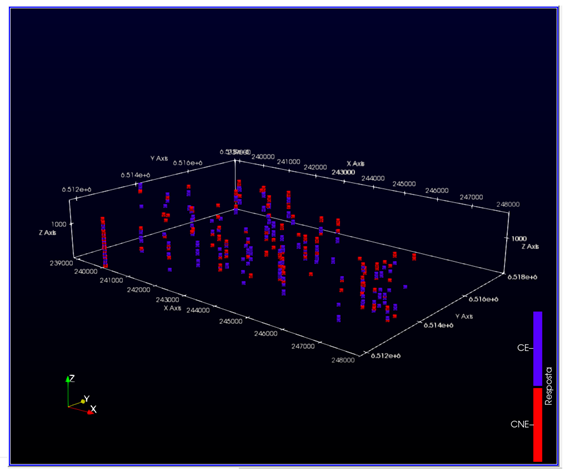
\includegraphics[scale=0.55]{./Capitulo_2/3d.png}	
	\caption{Informações de amostras obtidas em três dimensões. }
	\label{Fig_3d}
\end{figure}
\FloatBarrier

\section{Histograma}

A descrição das estatísticas das amostras é uma forma inicial para aglomerar um conjunto de informações extensos. Um gráfico de grande utilidade para verificar a frequência dos dados é o histograma. 

\begin{definition}[histograma]
	\textit{Um histograma é uma ferramenta gráfica, representada por um gráfico de barras que condiciona os valores de uma variável com suas frequências.}
\end{definition}

Esta ferramenta é essencial principalmente em três condições:

\begin{enumerate}
	\item \textbf{Classificação:} Quando possuímos classes distintas o histograma apresenta diretamente a proporção de cada classe considerada
	\item \textbf{Contagem:} Quando a variável constitui em valores inteiros, cada valor desta variável pode ser diretamente associada a sua frequência.
	\item \textbf{Contínuo:} Quando os valores são reais, podemos atribuir intervalos de classe ( ou em inglês \textit{bins}) aos quais estes valores estão inseridos. Dependendo do número de intervalos de classe e seu tamanho o histograma pode apresentar diferentes formas.
\end{enumerate}

Uma das proposições utilizadas para o cálculo do número ótimo de intervalos de classes é pela fórmula de Sturges \ref{equation_Sturges} 

\begin{equation}\label{equation_Sturges}
	\hat{h} = \frac{\text{amplitude dos dados}}{1+ log(n)}
\end{equation}
 
 Em que a amplitude dos dados é relacionado a diferença do máximo e do mínimo das amostras e $n$ é o número de amostras. A figura \ref{Fig3_1} representa um histograma da variável Cádmio do depósito de Jura. Podemos notar como a distribuição dos dados se comporta nesta variável, como aspectos de simetria, valores médios, e inclusive possíveis valores outliers, quando as barras de frequência são pequenas e distanciadas da maioria.

\FloatBarrier
\begin{figure}[!htb]
\centering
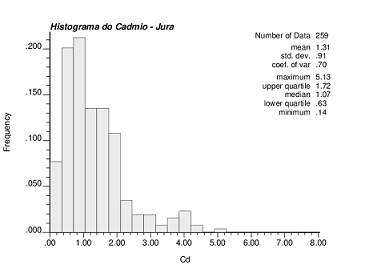
\includegraphics[scale=1]{./Capitulo_2/figura3_1.png}	
\caption{Histograma do Cd}
\label{Fig3_1}
\end{figure}
\FloatBarrier

A observação de uma frequência de uma classe é diretamente relacionada ao tamanho desta. Na figura \ref{Fig4_1} podemos ver que a classe de teores de $0,04$ a $0,75g/ton$ ocupa uma proporção de 20 \% dos dados.

\FloatBarrier
\begin{figure}[!htb]
\centering
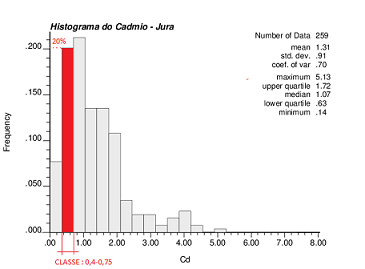
\includegraphics[scale=1]{./Capitulo_2/figura4_1.png}	
\caption{Histograma do Cd - Classe marcada}
\label{Fig4_1}
\end{figure}
\FloatBarrier

A construção de histogramas envolve sempre a criação de intervalos de classe de mesmo tamanho. Alterar apenas o tamanho de uma classe em detrimento de outras pode ser considerado um uso abusivo das estatísticas, enviesando a percepção de outras pessoas sobre as verdadeiras frequências dos dados. 

\begin{remark}
	Não é correto alterar o tamanho de apenas um intervalo de classe em detrimento dos outros. Esta prática é mal vista, e pode ser intuitivamente criada para gerar víes na percepção dos leitores quanto as frequências de determinados valores. 
\end{remark}

Assim como em outras estatísticas, a utilização dos histogramas favorece o entendimento global dos dados, mas prejudica no entendimento apurado da variável. A escolha do tamanho do intervalo é uma variável importante para a observação desta estatística gráfica. Valores de classe com tamanho muito grande apresentaram frequências maiores, mas perderão a forma natural dos dados. Valores de classe com tamanho muito pequeno apresentarão baixa frequência e se tornarão mais achatados, dificultando a visualização das proporções da variável. 

\begin{proposition}
	\textit{A escolha do tamanho do intervalo de classe é fundamental para verificar a forma do histograma e sua representação real. Valores de tamanho muito pequenos ou grandes podem gerar gráficos pouco intuitivos, escondendo a real simetria, valores médios e dispersão dos dados. É importante que um histograma caracterize visualmente os dados de forma a representar as estatísticas numéricas a serem calculadas.} 
\end{proposition}

Outra forma de representar um histograma é na sua forma acumulada. Neste caso cada valor das frequências de uma variável são aumentadas em ordem crescente, do menor valor das amostras até o maior valor. A figura \ref{Fig5_1} é uma demonstração do gráfico acumulado. 

\FloatBarrier
\begin{figure}[!htb]
\centering
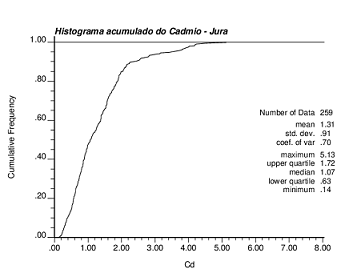
\includegraphics[scale=1]{./Capitulo_2/figura5_1.png}	
\caption{Histograma do Cd acumulado}
\label{Fig5_1}
\end{figure}
\FloatBarrier

A figura \ref{Fig6_1} demonstra a leitura do gráfico acumulado.Podemos notar por este gráfico que 60 por cento dos valores estão abaixo do teor de $1,5 g/tonelada$.  

\FloatBarrier
\begin{figure}[!htb]
	\centering
	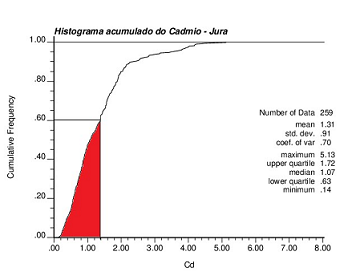
\includegraphics[scale=1]{./Capitulo_2/figura6_1.png}	
	\caption{Histograma do Cd acumulado - Leitura}
	\label{Fig6_1}
\end{figure}
\FloatBarrier

O formato dos histogramas pode adicionar importantes informações sobre a distribuição dos dados, como por exemplo a assimetria. Na figura \ref{Fig_simetric} podemos observar dois histogramas de depósitos minerais diferentes, um simétrico de Ferro em A) e um de alumínio assimétrico em B). Quando consideramos as técnicas clássicas de avaliação de depósitos a assimetria dos dados pode dificultar os métodos convencionais, o que torna depósitos de alta assimetria mais difíceis de reproduzirem estimativas condizentes.


\FloatBarrier
\begin{figure}[!htb]
	\centering
	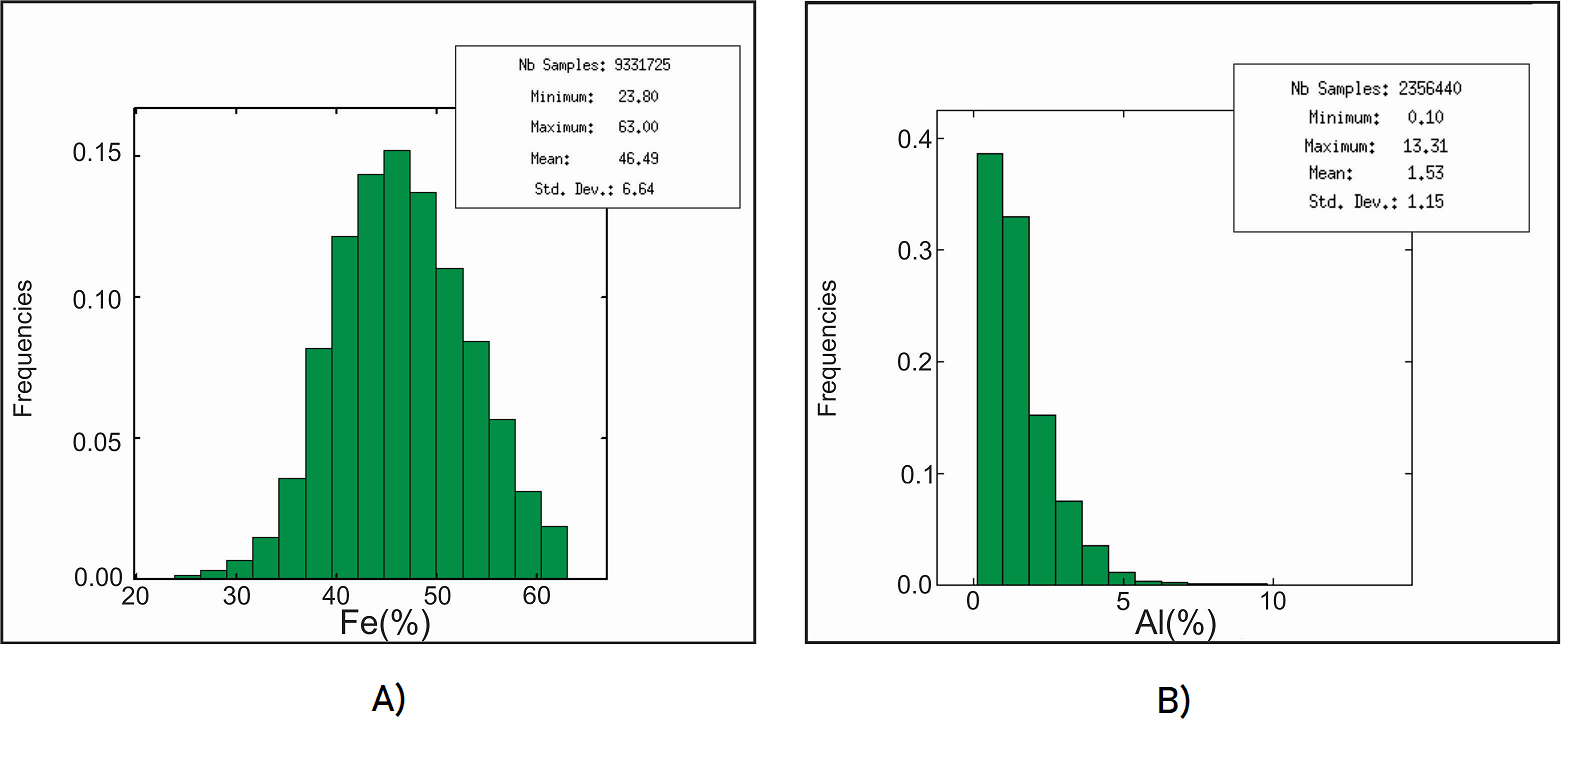
\includegraphics[scale=0.301]{./Capitulo_2/simetria.png}	
	\caption{Simetria para diferentes histogramas - a) histograma simétrico, b) histograma assimétrico}
	\label{Fig_simetric}
\end{figure}
\FloatBarrier

O formato do histograma também é um importante parâmetro para a inferência de distribuições de probabilidade. A partir dele podemos visualizar uma possível distribuição de probabilidade e dar um "chute" para testarmos se esta se encaixa na distribuição das amostras. Distribuições de frequências centradas podem ter como candidato um modelo de ajuste gaussiano, por exemplo. Distribuições assimétricas podem se encaixar, por exemplo, em um modelo lognormal.


\section {Inferência Estatística}

Após analisados os dados amostrais podemos utilizar funções para modelar populações dos dados. Na maioria dos casos não precisamos conhecer \textit{a priori} as distribuições da população, mas em alguns casos como na geoestatística não-linear, conhecer uma distribuição teórica de probabilidades pode facilitar estudos para entender problemas mais complexos

\begin{definition}[Inferência estatística]
	\textit{Inferência estatística é o método pelo qual deduzimos informações da população dos dados com base em informações das amostras}
\end{definition}
	
,
\subsection{Famílias de distribuições estatísticas}

Uma função de densidade de probabilidade de uma variável aleatória nada mais é do que uma função $p(X = x)$ que correlaciona cada realização $x$ da variável aleatória $X$ a uma dada probabilidade. Como consequência da definição algumas condições estão associadas:

\begin{itemize}
	\item $p(x) \leq 1 \forall x$
	\item $\int_{-\infty}^{\infty} p(x) dx = 1$ para distribuições contínuas
	\item $\sum_{x=-\infty}^{\infty} p(x) = 1$ em que a e b são limites para a distribuição discreta
\end{itemize}
 

\subsubsection{Distribuição de Poisson}

Esta é uma distribuição discreta amplamente utilizada para experimentos ditos de eventos "raros", ou seja, utilizada para modelar eventos que a probabilidade de ocorrência é diretamente proporcional ao tempo de espera. 

Em filas de caminhões, por exemplo, é muito comum a utilização da função de distribuição de Poisson para medir a probabilidade de chegada de um equipamento, pois é de se esperar que para um pequeno intervalo de tempo após a saída de um caminhão da frente de lavra, a probabilidade da chegada de outro  seja pequeno. Outro exemplo é a frequência de fraturas em uma rocha. É de se esperar que para tamanhos pequenos de rocha a quantidade de fraturas seja pequena, enquanto para tamanhos grandes de rocha essa densidade aumente.

A função de distribuição de Poisson pode ser escrita segundo a equação \eqref{equacao_de_Poisson}

\begin{equation}\label{equacao_de_Poisson}
P(X = x) = \frac{\exp^{-\lambda}\delta^{x}}{x!}
\end{equation}

Em que $x$ é uma realização da variável aleatória $X$, $P(X =x)$ é a probabilidade associada àquele evento e $\lambda = E(X)$ sendo o parâmetro da função. Na maioria dos casos aproximamos $E(X) \sim \bar{x}$. Tal como qualquer distribuição de probabilidades sabemos que a soma de todos os eventos possíveis deve gerar um resultado igual a 1. Podemos demonstrar isso de acordo com a prova 


\begin{proof}
	Sabendo que a função exponencial pode ser aproximada por uma série de Taylor como a seguir temos :
	\begin{align*}
	&e^{\lambda} = \sum_{n= 0}^{\infty} \frac{\lambda^{x}}{x!}\\
	&\text{Então:} \\
	&\sum_{x=0}^{\infty} P(X=x) = \sum_{x=0}^{\infty} \frac{\exp^{-\lambda}\lambda^{x}}{x!}\\ 
	&\sum_{x=0}^{\infty} P(X=x) = \exp^{-\lambda}\sum_{x=0}^{\infty} \frac{\lambda^{x}}{x!}\\
	&\sum_{x=0}^{\infty} P(X=x) = \exp^{-\lambda}\exp^{\lambda} = 1\\
	\end{align*}
\end{proof}

 
\subsubsection{Distribuição Gaussiana }

Esta talvez seja uma das funções de densidade de probabilidade mais populares e representa um grande papel na geoestatística. As equações de estimativa lineares que serão apresentadas neste livro são também analogamente chamadas de \textbf{equações normais}. Isto se deve pelo fato de que os resultados obtidos em variáveis gaussianas são os mais precisos possíveis dentro de todas outras distribuições na geoestatística. Quanto mais próximo for a distribuição das amostras de uma distribuição gaussiana, melhores serão os resultados de uma estimativa geoestatística.

\begin{proposition}
	\textit{Consideremos uma variável Z, gaussiana e estacionária ( em prática a variável que pode ser aproximada de um histograma por uma gaussiana), com média $m$ e variância $\sigma{2}_{y}$, a hipótese de permanência da normalidade indica que uma variável Y estimada segue uma distribuição de mesma forma e média $m= E(Z) = E(Y)$ e variância $\sigma{2}_{Z} \neq \sigma{2}_{Y}$} -\cite{journel1978mining}
\end{proposition}

O formato de uma distribuição gaussiana é tipicamente na forma de um sino (\textit{bell shape}), centrado em um valor médio e com uma variância característica. A figura \ref{Fig_gaussian} demonstra uma distribuição gaussiana típica com média igual a 5 e variância igual a 2.

\FloatBarrier
\begin{figure}[!htb]
	\centering
	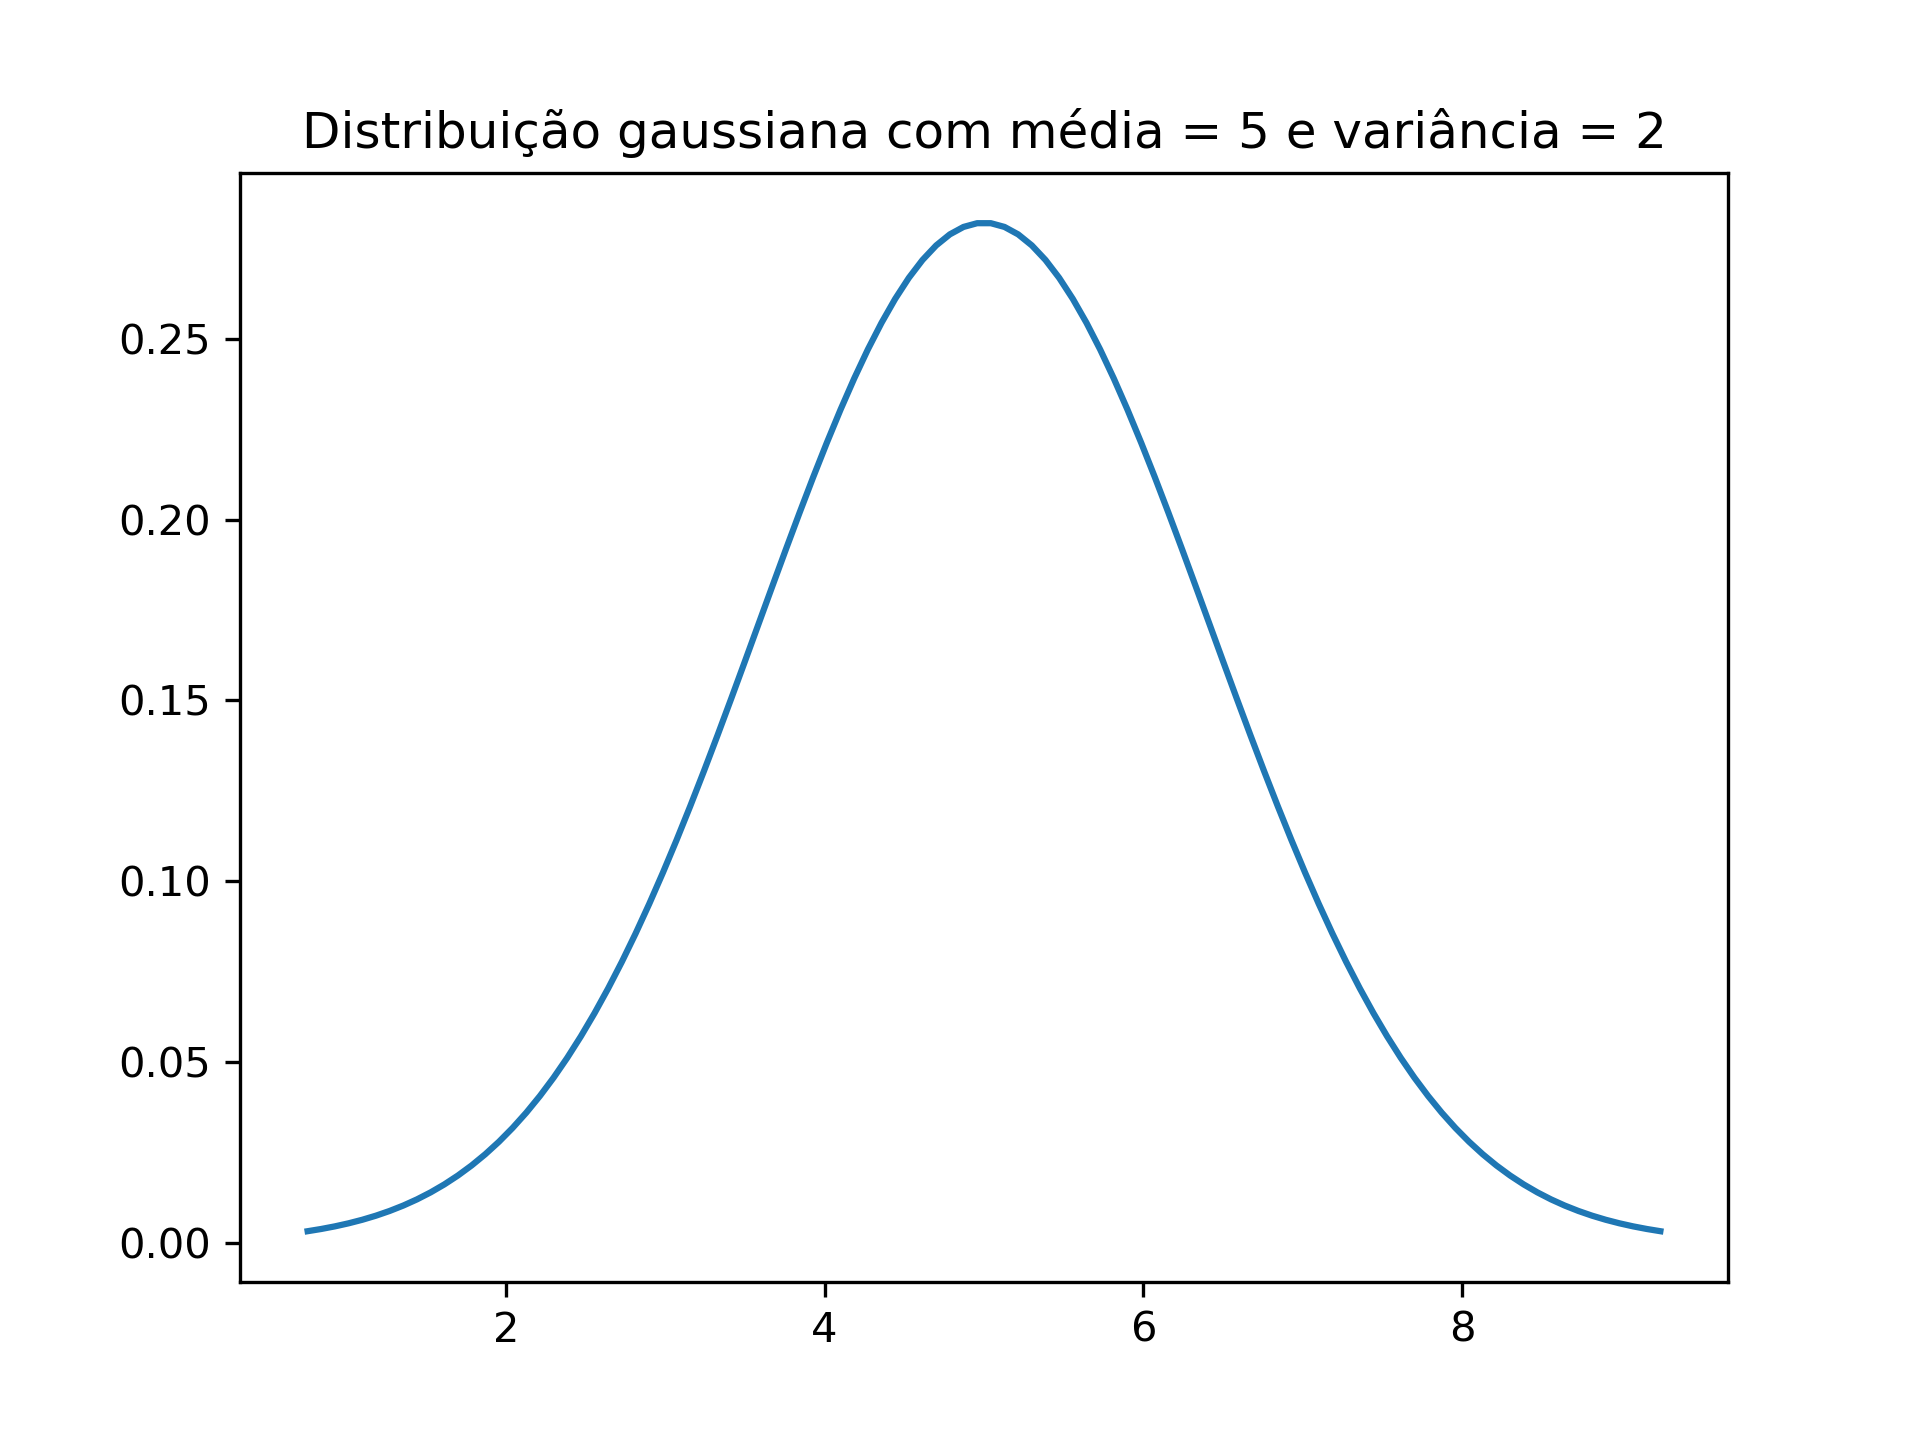
\includegraphics[scale=0.9]{./Capitulo_2/gaussian.png}	
	\caption{Forma de uma distribuição gaussiana com média 5 e variância 2}
	\label{Fig_gaussian}
\end{figure}
\FloatBarrier


A distribuição é um modelo simétrico e descrito por dois parâmetros, a média da população e a variância. A função de densidade de probabilidade da distribuição pode ser desrita segundo a equação \eqref{equacao_de_Gaussiana}


\begin{equation}\label{equacao_de_Gaussiana}
P(X = x) = \frac{1}{\sqrt{2\pi\sigma}}exp^{-\frac{(x-\mu)^2}{2\sigma^2}}
\end{equation}

Em que $\sigma^2$ é a variância da distribuição aleatória e $\mu$ é a média. O caso particular da distribuição gaussiana é quando sua média é igual a zero e variância é igual a 1, neste caso temos uma distribuição padronizada segundo a equação \eqref{equacao_de_Gaussiana_padr}

\begin{equation}\label{equacao_de_Gaussiana_padr}
P(X = x) = \frac{1}{\sqrt{2\pi}}exp^{-\frac{(x)^2}{2}}
\end{equation}

Uma variável aleatória pode ser padronizada segundo a relação \eqref{padronizacao_var}

\begin{equation}\label{padronizacao_var}
X_{p} = (X-\mu)/\sigma
\end{equation}

Que nada mais é do que uma operação de deslocamento da variável aleatória pela sua média e encurtamento da distribuição pelo seu desvio padrão.

Para demonstrar que a distribuição gaussiana possui soma de todos os seus eventos igual a 1 devemos antes lembrar que ela é uma distribuição simétrica, logo a soma dos valores à esquerda do valor médio da distribuição é idêntico à soma dos valores à direita da distribuição. A integral da função gaussiana não possui uma antiderivada para utilizarmos explicitamente, por isso o truque utilizado é provar que o quadrado da integral da gaussiana é equivalente a $2\pi$. Logo temos:


\begin{proof} \label{prova_gauss}
	Prova do somatório de uma função gaussiana ser igual a 1
	\begin{align*}
	&Int^{2} = \left(\int_{-\infty}^{\infty} e^{-\frac{(x)^{2}}{2}}dx\right)^{2} = 4\int_{0}^{\infty} e^{-\frac{(t)^2}{2}}dt \int_{0}^{\infty} e^{-\frac{(u)^2}{2}}du\\
	&4\int_{0}^{\infty}\int_{0}^{\infty}e^{\frac{-(t^2+u^2)}{2}}dt du\\
	&\text{Alterando para coordenadas polares}\\
	&4\int_{0}^{\infty}\int_{0}^{\pi/2}re^{\frac{-r^{2}}{2}}drd\theta \\
	&2\pi\int_{0}^{\infty}re^{\frac{-r^{2}}{2}}dr \\
	&2\pi\\
	&\text{Logo se: }Int^{2} = 2\pi\\
	&Int = \sqrt{2\pi}\\
	&\text{portanto :} \\
	&\frac{1}{\sqrt{2\pi}} \int_{-\infty}^{\infty} e^{-\frac{x^{2}}{2}}dx = \frac{1}{\sqrt{2\pi}}\sqrt{2\pi} = 1\\
	\end{align*}
\end{proof}

\subsubsection{Distribuição Lognormal}

A distribuição lognormal é uma distribuição assimétrica e positiva, geralmente associada na mineração com depósitos de elementos raros , tais como ouro, diamante e platina. Pode ser considerada uma distribuição cujo seu logaritmo é normalmente distribuído. A equação \eqref{equacao_lognormal} demonstra a função de densidade de probabilidade para a distribuição lognormal.

\begin{equation}\label{equacao_lognormal}
P(X = x) = \frac{1}{\sqrt{2\pi\sigma}}\frac{1}{x}exp^{\frac{(-log(x))^2}{2}}
\end{equation}

O Valor esperado da distribuição pode ser demonstrado segundo a equação \eqref{Valor_esp_equacao_lognormal}

\begin{equation}\label{Valor_esp_equacao_lognormal}
E(X) = e^{\mu + \frac{\sigma^2}{2}}
\end{equation}

A figura \ref{Fig_lognorm} apresenta a forma assimétrica da distribuição lognormal, para um distribuição com média 5 e variância igual a 2.

\FloatBarrier
\begin{figure}[!htb]
	\centering
	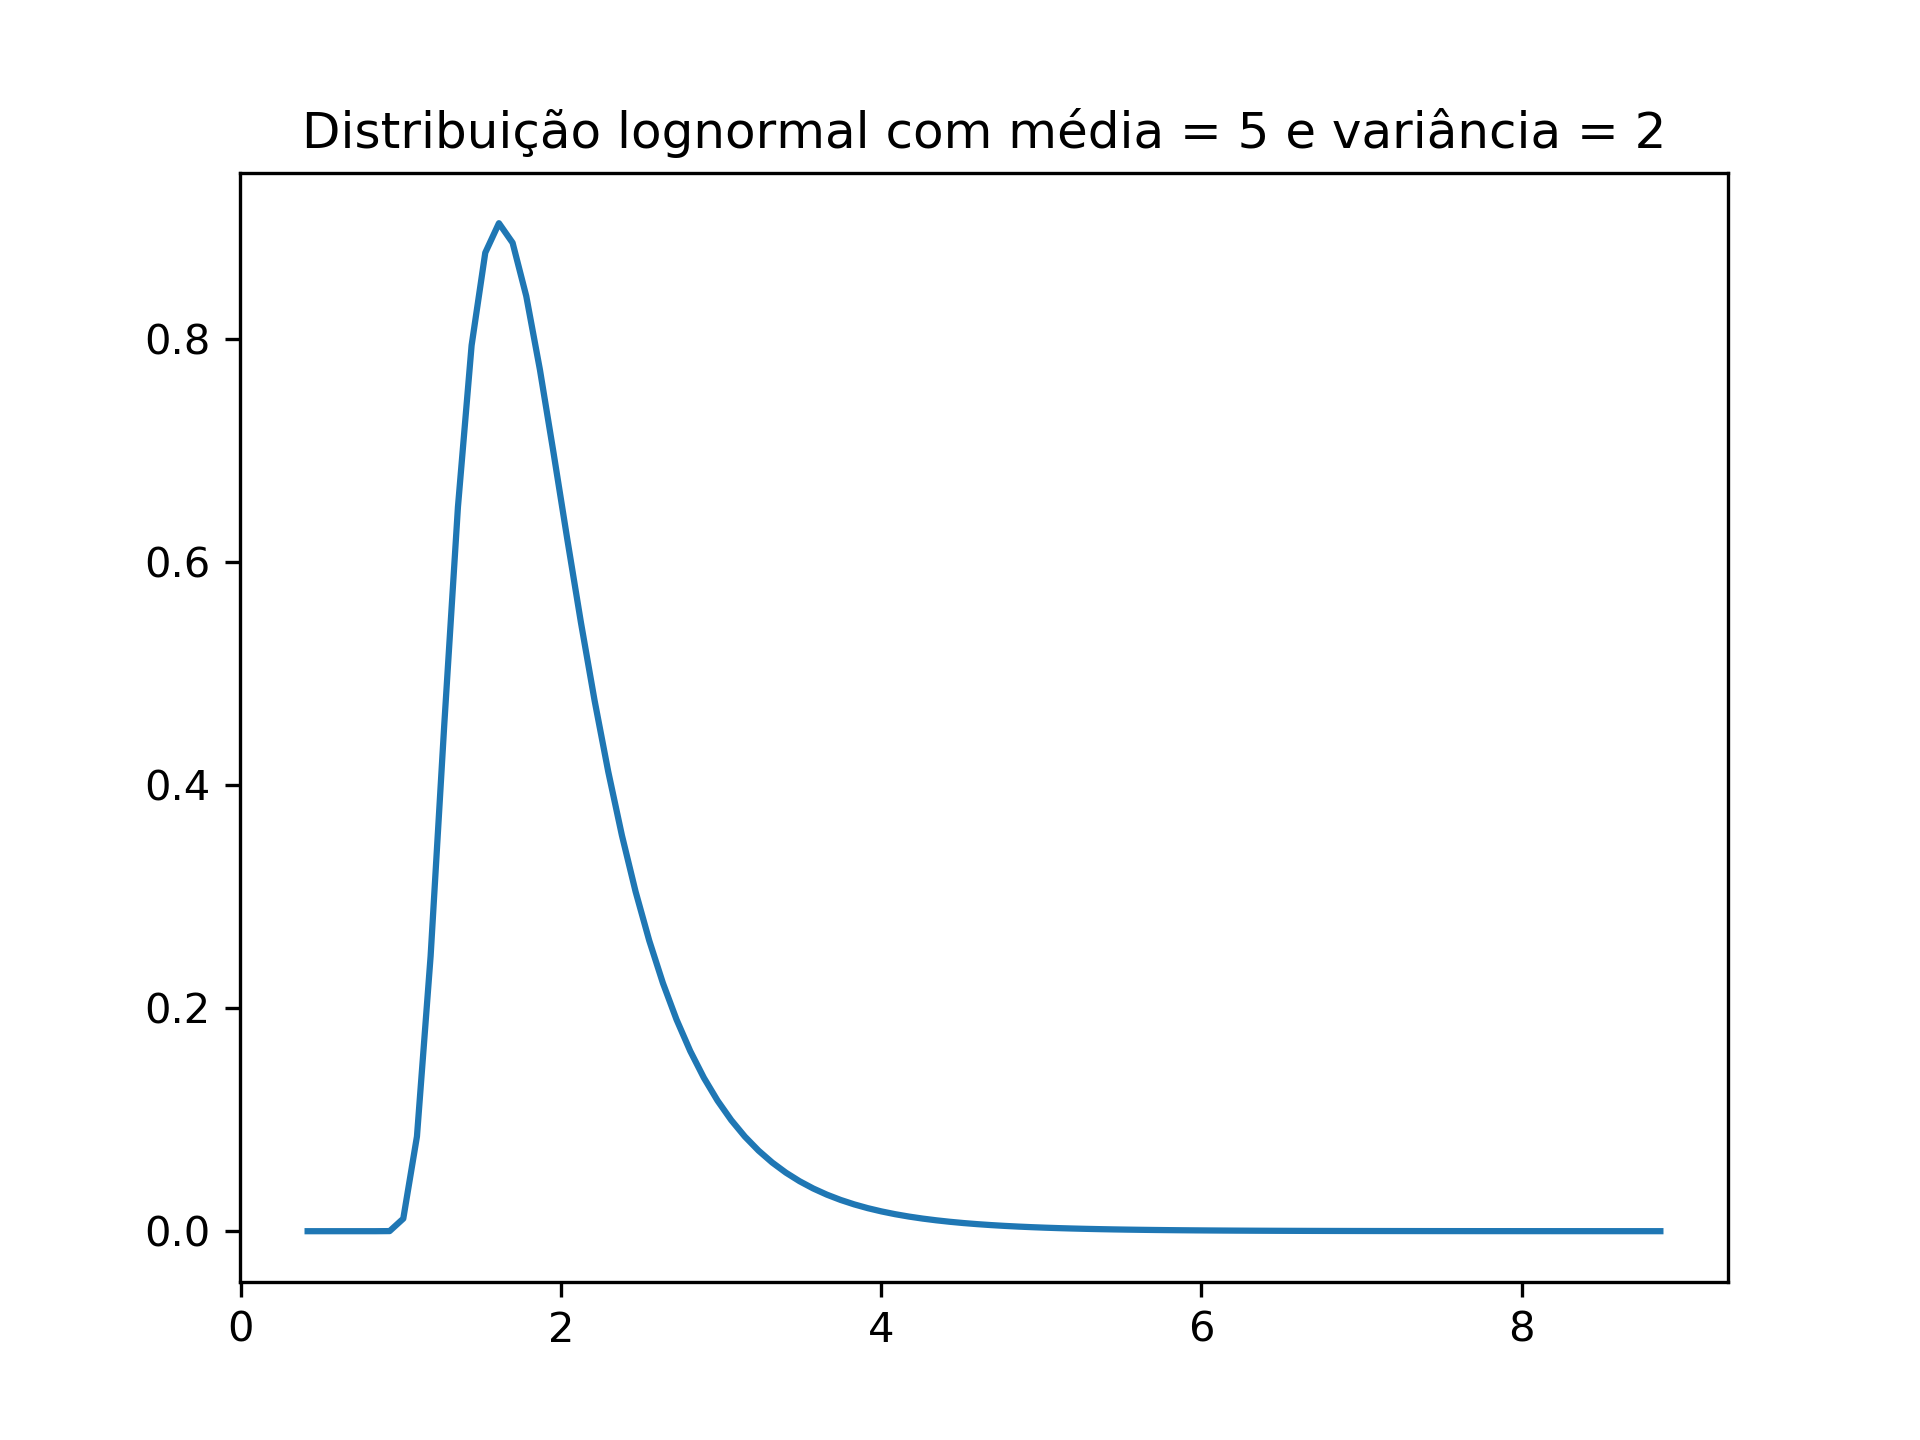
\includegraphics[scale=0.9]{./Capitulo_2/lognormal.png}	
	\caption{Forma de uma distribuição lognormal com média 5 e variância 2}
	\label{Fig_lognorm}
\end{figure}
\FloatBarrier



\subsubsection{Estimando a média da população }

O processo de inferência estatística resume-se em determinar características da população a partir de dados amostrais. Podemos estimar o valor real da média da função aleatória $Z(x)$ a partir do estimador $\hat{Z}(x)$ a partir  da média aritmética $\sum_{i=1}^{n} Z(x_{i})/n$  em que $n$ constitui um número grande de variáveis aleatórias em diferentes suportes $i$. A equação \eqref{Media_amostra} apresenta este processo. 

\begin{equation}\label{Media_amostra}
E(\hat{Z}(x)) = E\left(\sum_{i=1}^{n} Z(x_{i})\right)/n= \left(\sum_{i=1}^{n} E(Z(x_{i}))\right)/n = \left(\sum_{i=1}^{n} m\right)/n = m
\end{equation}

Sobre a hipótese de estacionaridade da média, sabemos que a média das variáveis aleatórias é igual a média da função aleatória. Ou seja, sob a hipótese de estacionaridade de segunda ordem podemos considerar que a média das amostras é um bom estimador para a média da população ou do depósito mineral. 

Enquanto a variância no entanto temos segundo a equação \eqref{Var_amostra}

\begin{equation}\label{Var_amostra}
Var(m) = Var\left(\sum_{i=1}^{n} Z(x_{i})/n\right) = \sum_{i=1}^{n} 1/n^2Var\left(Z(x_{i})\right)= \sigma^2/n
\end{equation}

Em outros termos, sob a hipótese de estacionaridade, a variância da média populacional tende a reduzir de acordo com o número de amostras tomadas. Isso também é chamado de efeito de suporte, pois quanto mais informações temos com a amostragem, mais o valor esperado de uma função aleatória tende a ser o correto. Quanto maior a quantidade de amostras utilizadas em uma estimativa, menores serão os erros associados a esta estimativa média local. A figura \eqref{Efeito_Suporte} demonstra como o valor médio tende a cada vez se aproximar mais da média das amostras com o aumento do número de amostras.

\begin{figure}[H]
 	\centering
 	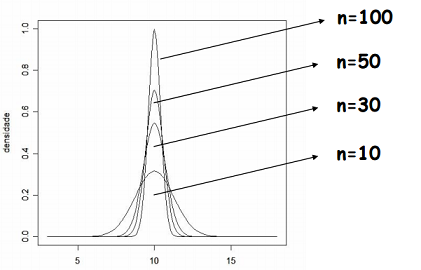
\includegraphics[scale=1.0]{./Capitulo_2/EfeitoSuporte.png}	
 	\caption{Figura demonstrando o efeito de suporte para um número crescente de amostras. O aumento do número de amostras tende a concentrar a  função de densidade de probabilidade entorno do valor médio }
 	\label{Efeito_Suporte}
\end{figure}

\section{Distribuição t-Student} 

Para determinarmos a distribuição gaussiana geralmente assumimos o conhecimento a respeito da variância da população. Se considerarmos a \textbf{distribuição de valores médios}, sabemos que se $Z_{x1}, Z_{x2}, ... , Z_{xn}$ são amostras normalmente distribuidas normalmente $\phi(m, \sigma^{2})$, então a quantidade 

\begin{equation}\label{padronizacao_var}
Z_{p} = \frac{(\bar{Z(x)}-\mu)}{\sigma/\sqrt{n}}
\end{equation}

É distribuída com variável aleatória $\phi(0,1)$. A distribuição dos valores médios $(\bar{Z(x)}-\mu)/(\sigma/\sqrt{n})$ segue a distribuição chamada de t-Student, com $n-1$ graus de liberdade. Quando o número de amostras tende a crescer, aproximadamente de 30, a distribuição t-Student converge para a distribuição normal padrão $\phi(0,1)$. Por isso dizemos que para estudos estatísticos iniciais, precisamos de pelo menos 30 amostras para se ter uma melhor compreensão da média. 

\section{Dimensionamento de malhas regulares} 

Em campanhas de prospecção preliminares é rotineiro utilizar técnicas estatísticas convencionais para estimar o tamanho e posicionamento de malhas de amostragem. No estágio inicial é necessário cobrir uma certa área de forma a verificar suas potencialidades. A medida que os estudos avançam, as amostragens tendem a aumentar e se tornarem mais densas, e estudos geoestatísticos mais avançados são realizados. A área de influencia de uma perfuração pode ser calculada pela equação \eqref{area_influ}

\begin{equation}\label{area_influ}
A_{0} = \frac{A}{n}
\end{equation}

Os  estudos iniciais são fortemente afetados pela regularidade do depósito mineral. Depósitos erráticos como veios de ouro tendem a necessitar de malhas mais adensadas que depósitos regulares como os de carvão mineral.

\begin{remark}
	\textit{O principal fator que controla a densidade da malha de perfuração é a regularidade do depósito e, por isso, a malha tem de ser cada vez mais densa, à medida que trabalham depósitos onde a variabilidade na forma ou qualidade (teor e conteúdo) é maior} - \cite{maranhao1985introduccao} 
\end{remark}

Para encontrarmos o número mínimo de amostras segundo o erro esperado para amostragem, utilizamos a equação

\begin{equation}\label{area_influ}
N = \frac{(t.CV)^2}{E^{2}}
\end{equation}

Em que $t$ é o valor da variável t-Student para um nível de confiabilidade, $CV$ é o valor do coeficiente de variação do depósito mineral e $E$ é o valor do erro aceitável para a estimativa. 

\begin{proposition}
	\textit{Considere um depósito mineral com coeficiente de variação igual a 51,98\%, um valor de confiabilidade para a média de 95\% (t-student = 2.20, para 12 amostras), e um erro aceitável para uma medida de no máximo 20\%. A área pesquisada é igual a $70.000m^{2}$, e realizaremos 12 amostras. Logo o erro que cometeremos é $E=\sqrt{\frac{(t.CV)^{2}}{N}} = \sqrt{\frac{(2.20t.51.98)^{2}}{12}}= 32.7\%$}
\end{proposition}

\section{Exercícios}

\begin{exercise}
	Considere o conjunto de amostras com teores de ferro contendo unicamente hematita $Fe_{2}O_{3}$ e sílica $SiO_{3}$. Os valores são $\left(45,69,80,35,56,78\right)\%$. Determine os valores outliers do problema considerando a massa atômica do ferro igual 56g/mol e do oxigênio igual a 16g/mol. Resp.: 80\% e 78\%
\end{exercise}
\begin{exercise}
	Considere o conjunto de amostras com teores $\left(2.4,5.0,7.6,4.3,2.7,8.9\right)$ g/ton todos com o mesmo suporte. Encontre o valor da média, da variância, do desvio padrão do conjunto de amostras. Resp.: $\bar{x}= 5.7$ ,$s^2 = 5.06$ , $s = 2.25$
\end{exercise}
\begin{exercise}
	Um geólogo precisa decidir entre duas metodologias de amostragem para um dado elemento de pesquisa. Entre elas temos a sonda diamantada e o pó de perfuratriz. As incertezas do custo da pesquisa estão diretamente relacionadas com a variabilidade da recuperação, desejando o método com o menor risco associado . Para isso mediu-se a recuperação dos testemunhos e do pó retirado pela máquina. A recuperação dos testemunhos fora de 90\% com um desvio padrão de 30\%, enquanto a do pó foi de 70\% com uma variação de 20\%. Deseja-se saber qual método utilizar. Resp.: Pó de perfuratriz << CV
\end{exercise}
	
	 


\chapter{Estatística bivariada}

\begin{myquoting}{Sherlock Holmes em 'Um estudo em Vermelho'}
	
	Como em outras artes,  a ciência da dedução e análise é uma que não pode ser adquirida por um longo e paciente estudo, nem é a vida longa o suficiente para permitir qualquer mortal se ater a mais alta perfeição nela.  
\end{myquoting}

\section{Introdução}

Na análise de bancos de dados geralmente se torna necessário comparar duas populações diferentes. Em um depósito mineral, por exemplo, podemos ter diversas variáveis presentes. Em alguns casos a relação entre elas pode ser um indício dos fenômenos genéticos de formação das rochas. Em outros casos apenas estamos interessados em como uma informação secundária pode estar relacionada com uma primária de interesse. Seria proveitoso para nós, por exemplo, traçar um modelo que definisse a chance de obter uma amostra com certo teor em contrapartida de outra amostra com o teor de uma variável diferente. Em um depósito vulcanogênico sulfetado podemos estar interessados em prever a quantidade de um elemento metálico a partir do enxofre da rocha encaixante. Enfim, toda a informação que relaciona duas variáveis pode ser descrita pela estatística bivariada.  

Diferentemente da estatística univariada, a comparação de histogramas de variáveis diferentes não é uma alternativa interessante sobre o ponto de vista prático. É muito difícil determinar a relação entre duas amostras simplesmente pelas suas proporções individuais. Para isso definimos algumas ferramentas que facilitam ao modelador entender a relação entre duas variáveis distintas visualmente e numericamente. 

As seções que se prosseguem mostrarão algumas das ferramentas utilizadas para se caracterizar distribuições bivariadas. Inicialmente apresentamos as \textbf{ferramentas gráficas} mais utilizadas e depois algumas \textbf{estatísticas pontuais} utilizadas. 

\section{Probabilidade condicional e Esperança condicional} 

\subsection{Probabilidades condicionais e conjuntas}

Probabilidades não são nada além de métricas de conjuntos, proporções de acordo um espaço amostral ($\Omega$). Estas proporções podem tomar diferentes características quando analisamos não apenas um conjunto individual, mas a interação entre eles. Muitas vezes não estamos interessados em determinar as probabilidades ou frequências individuais de uma variável aleatória. É interessante, por exemplo, determinar combinações entre variáveis e suas possíveis relações. E se desejarmos saber qual é a frequência de um minério e que seu conteúdo tenha um determinado valor de impureza? Se denotarmos $X$ como o evento de ser minério, e $Y$, a variável que denota seu limite de impurezas, podemos denotar a probabilidade de $P(X,Y)$ como sendo a probabilidade de que \textit{"Um material seja minério e apresente impurezas acima do limite desejado"}. A forma mais simples de se entender probabilidades é de acordo com um diagrama de Venn, como na figura \ref{disjuntos}

\FloatBarrier
\begin{figure}[!htpb]
	\centering
	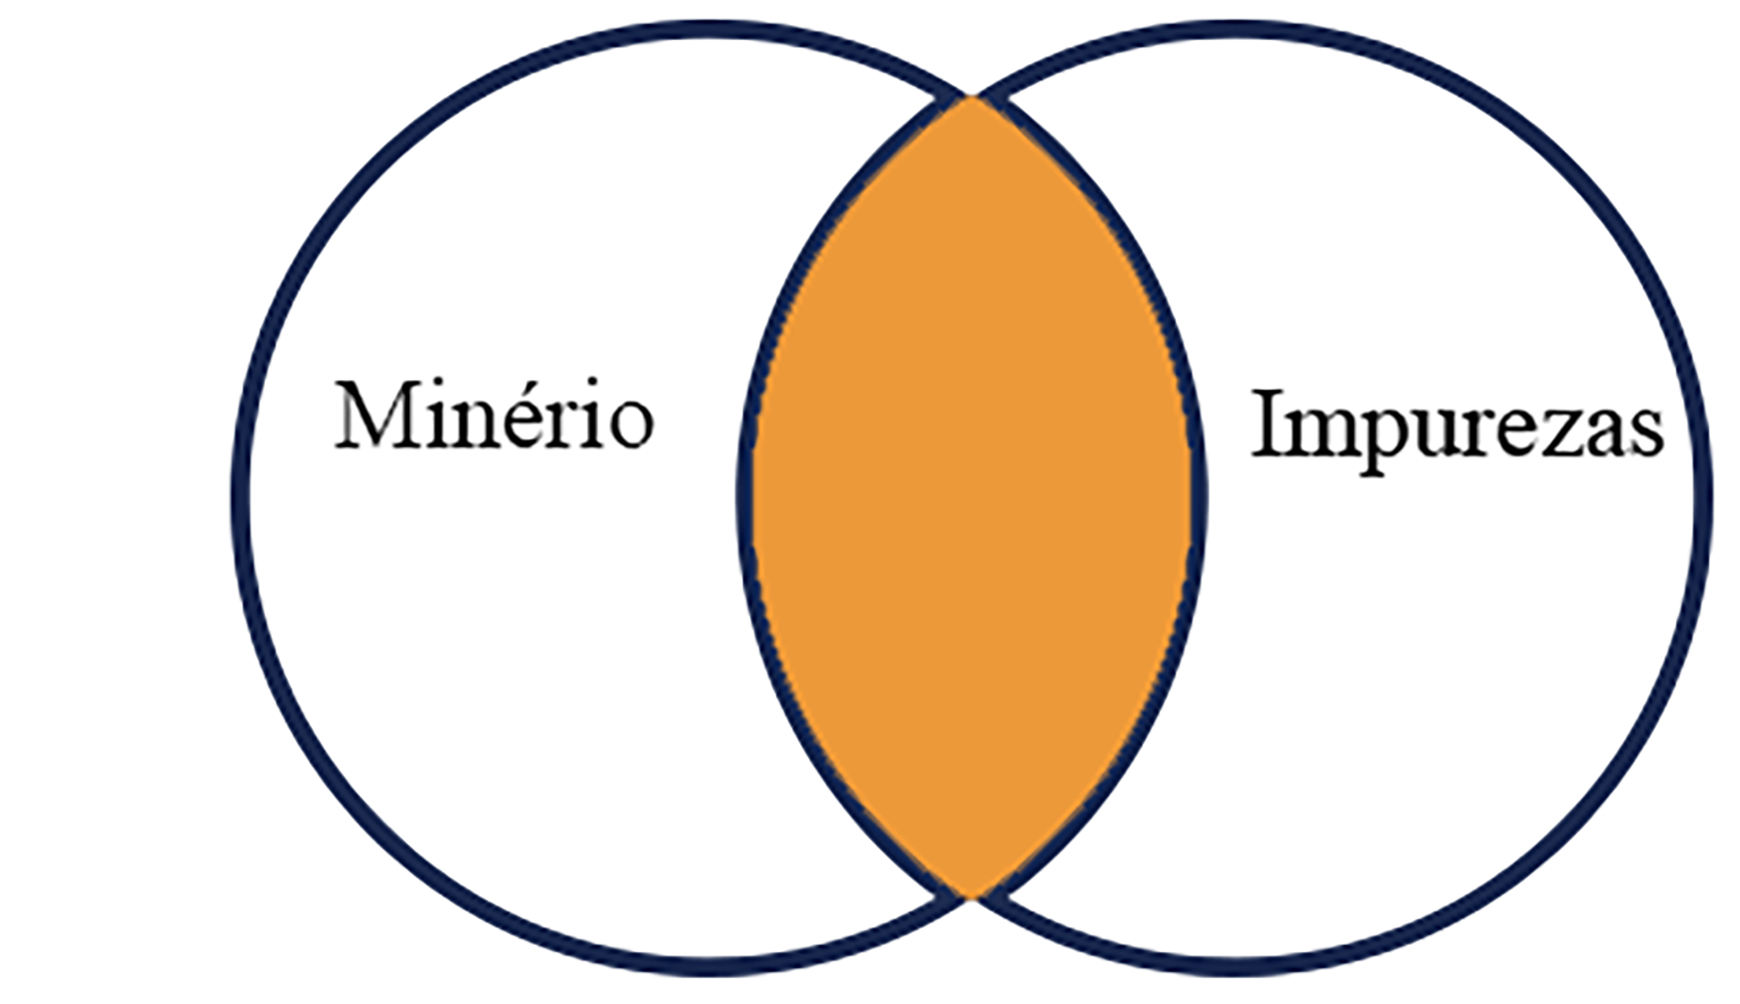
\includegraphics[scale=0.4]{./Capitulo_3/DISJUNTO.png}	
	\caption{Demonstração de eventos disjuntos entre a variável minério e impureza a partir de um diagrama de Venn. Nota-se a área laranja como sendo a interseção dos eventos representado pela probabilidade $P(X,Y)$ }
	\label{disjuntos}
\end{figure}
\FloatBarrier

Observe a tabela \ref{tabela_impureza}. Notamos na coluna três o número de vezes que o minério considerado possui uma impureza maior ou igual a 0,005. Neste caso sabemos que há 2 valores em cinco em que isso ocorre. Logo a probabilidade conjunta é P(Minerio) $\bigcap$ P(Impureza $\geq$  0.005) = 2/5 = 40\%

\FloatBarrier
\begin{table}[!htpb]
	\centering
	\caption{Tabela da relação entre um dado minério e uma impureza}
	\label{tabela_impureza}
	\begin{tabular}{ccc}
		\toprule
		Minério & Impureza & Minério $\bigcap$ (Impureza \textgreater=0,005) \\ \midrule
		Sim     & 0,005    & 1                                                           \\
		Não     & 0,007    & 0                                                           \\
		Não     & 0,008    & 0                                                           \\
		Sim     & 0,006    & 1                                                           \\
		Sim     & 0,003    & 0                                                           \\ \bottomrule
	\end{tabular}
\end{table} 
\FloatBarrier

Em alguns casos também é importante determinar a conjunção entre os eventos, ou a probabilidade de $P(X \vee Y)$. Neste caso queremos determinar \textit{"Um material seja minério ou apresente impurezas acima do limite desejado"}. Note que a conjunção 'ou' é um conectivo lógico muitas vezes díspare do seu uso corriqueiro no português. Ser um ou outro na verdade não é uma escolha entre um dos elementos, mas uma soma dos eventos. A representação da conjunção pode ser vista na figura \ref{conjuncao}.

\FloatBarrier
\begin{figure}[!htpb]
	\centering
	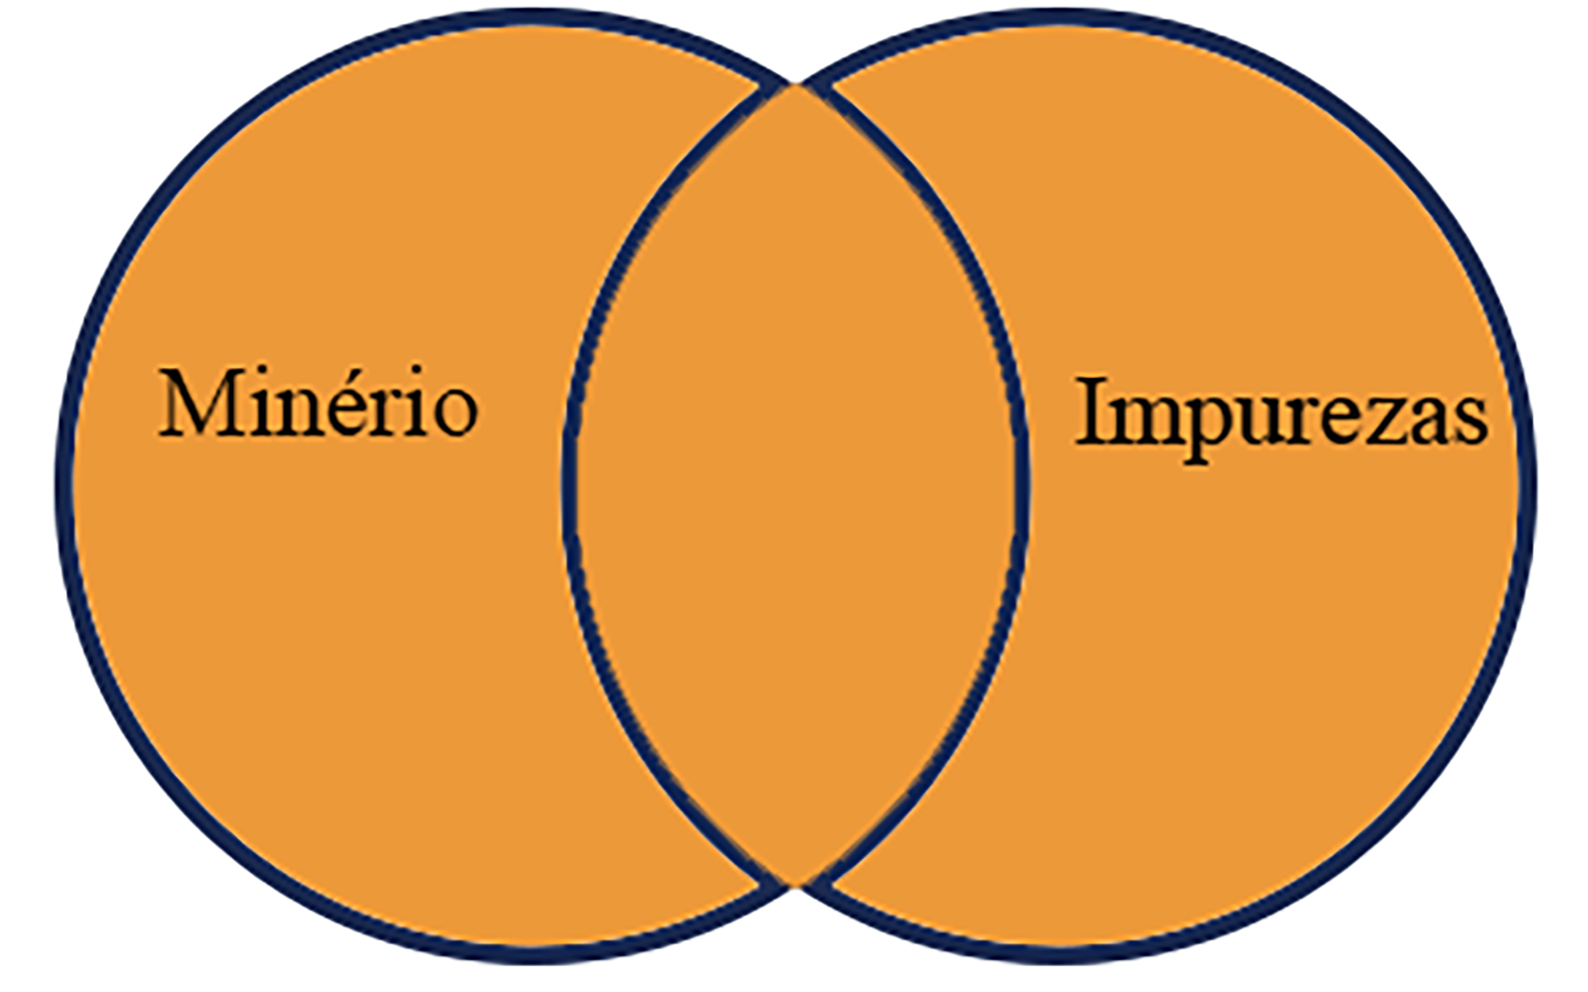
\includegraphics[scale=0.4]{./Capitulo_3/conjucao.png}	
	\caption{Demonstração da conjunção de eventos entre a variável minério e impureza a partir de um diagrama de Venn. Nota-se a área laranja como sendo a interseção dos eventos representado pela probabilidade $P(X\vee Y)$ }
	\label{conjuncao}
\end{figure}
\FloatBarrier

Estas relações lógicas envolvem o conhecimento entre os eventos independentemente. Conhecer $P(X,Y)$ é examente o mesmo que conhecer $P(B,A)$. Em alguns casos devemos entender o conceito de dependência na estatística, expresso pela probabilidade condicional. Neste caso queremos saber \textit{"dado que um material apresente impurezas, qual é sua probabilidade de ser minério"}. Esta é uma afirmação muito diferente da obtida nos outros casos, pois para sabermos se algo é minério, precisamos saber antes se ele contém impurezas. A probabilidade condicional $P(X|Y)$ pode ser demonstrada pela  figura \ref{disjuntos2} como a relação da área laranja pela área hachurada.

\FloatBarrier
\begin{figure}[!htpb]
	\centering
	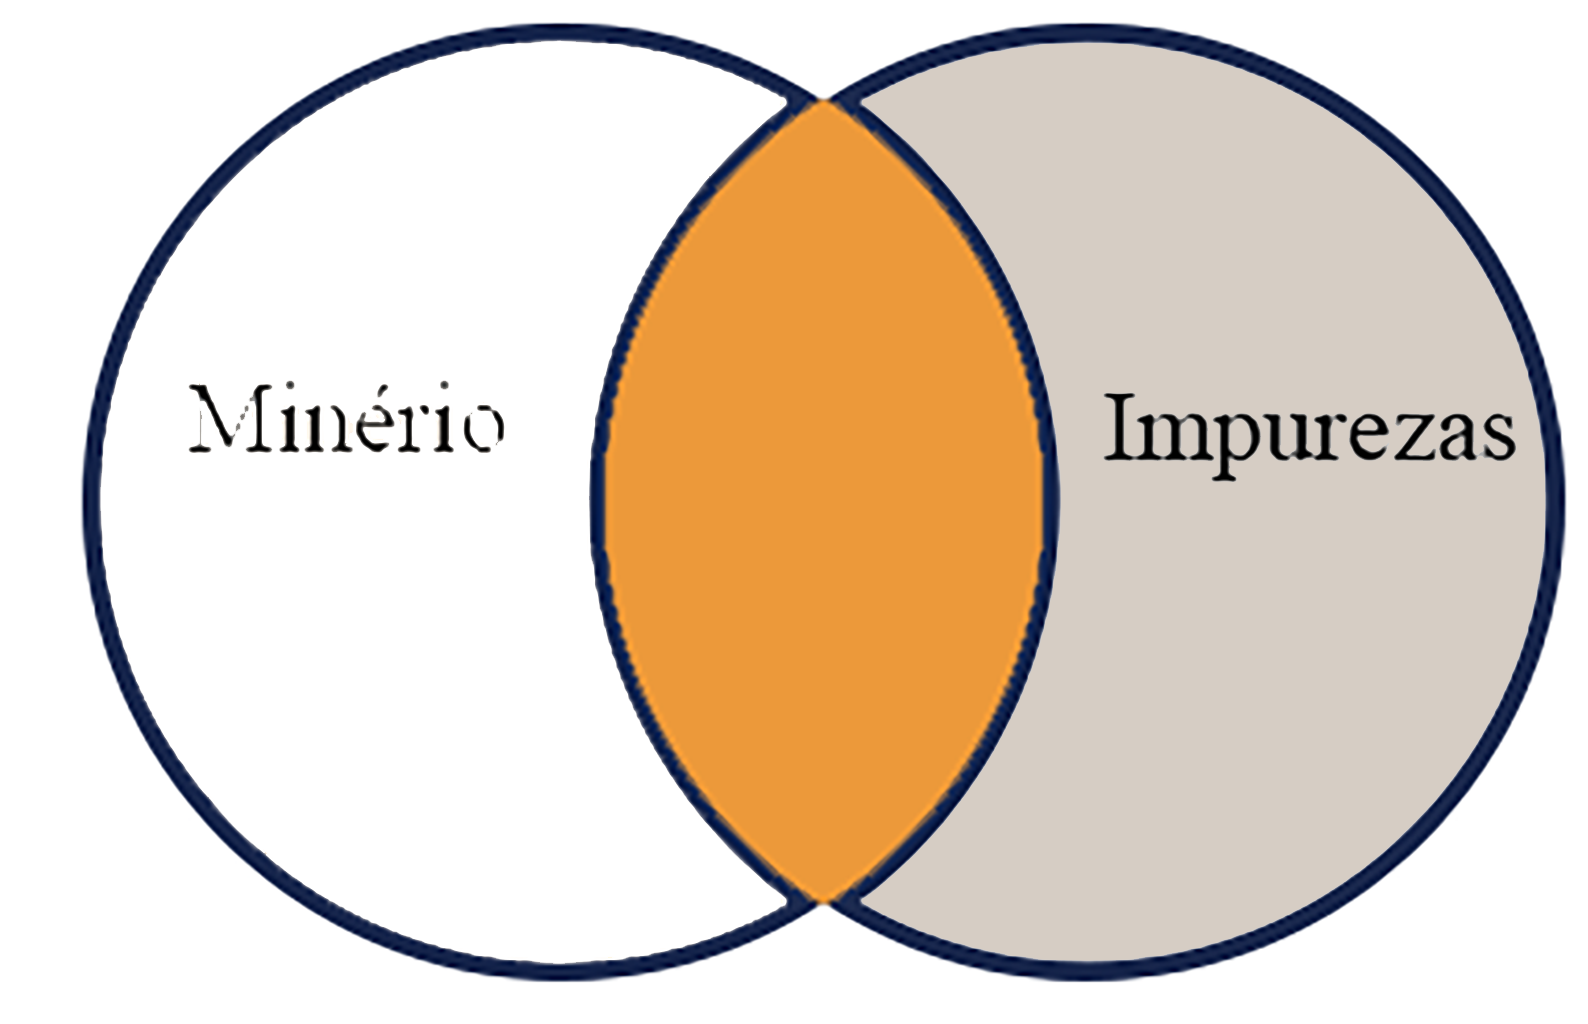
\includegraphics[scale=0.4]{./Capitulo_3/DISJUNTO_2.png}	
	\caption{Demonstração da probabilidade condicional entre a variável minério e impureza a partir de um diagrama de Venn.Nota-se a área laranja como sendo a interseção dos eventos disjuntos. A probabilidade condicional é a relação entre a área laranja pela área hachurada. }
	\label{disjuntos2}
\end{figure} 
\FloatBarrier

Esta relação também é chamada de teorema de Bayes, e envolve a equação \eqref{Bayes}

\begin{equation}\label{Bayes}
P(X|Y) = \frac{P(X,Y)}{P(Y)}
\end{equation}

\begin{proposition}
	\textit{As probabilidades condicionais expressam um importante conceito na geoestatística, a dependência entre variáveis aleatórias. Quando estudamos fenômenos espaciais, os valores obtidos em um suporte específico $x_{1}$ são muito mais dependentes de $x_{2}$ do que $x_{3}$, se a distância de $\left\{ x_{1},x_{2} \right\}$ for menor que a distância de $\left\{ x_{1},x_{3} \right\} $} 
\end{proposition}

\subsection{Esperança condicional}

A partir da definição de probabilidade condicional também é possível determinar a esperança condicional. Ela nada mais é que o valor médio obtido e uma variável $Y$ dado que a variável $X$ assuma um valor específico $x$. Por exemplo, podemos determinar qual é a probabilidade do material ser contaminado $Y$, dado que a presença de um litotipo $X$ seja $x =\{itabirito\}$, de acordo com a equação \eqref{pcond}.  

\begin{equation}\label{pcond}
E(Y|X=x) = \sum_{y \in Y} y P(Y =y|X=x)
\end{equation}

Considere que $Y$ seja uma variável binária tal que assuma o valor $0$ para o elemento contaminado, e valor $1$ para não contaminado. A variável $X$ pode assumir os valores de itabirito e calcário no problema. Analisando a tabela \ref{tabela_condic} podemos determinar as probabilidades de acordo com os respectivos valores apresentados. 


\FloatBarrier
\begin{table}[!htpb]
	\centering
	\caption{Tabela da relação entre um minério contaminado e litotipo}
	\label{tabela_condic}
	\begin{tabular}{cccc}
		\toprule
		Y & X & (Y=0| X=itabirito ) & (Y=1| X=itabirito)  \\ \midrule
		contaminado         & itabirito    & 1    &0                                                       \\
		descontaminado     & calcário     & 0    &0                                                       \\
		descontaminado     & calcário     & 0    &0                                                       \\
		contaminado         & itabirito    & 1    &0                                                       \\
		descontaminado     & itabirito    & 0    &1                                                       \\ \bottomrule
		P(Y=y|X=x) 		&              &2/3   &1/3													   \\ \bottomrule
	\end{tabular}
\end{table} 
\FloatBarrier

O valor esperado condicional pode ser obtido a partir da tabela pode ser calculado por \eqref{result}

\begin{equation}\label{result}
E(Y|X=itabirito) = 2/3.0 + 1/3.1 = 1/3
\end{equation}

No caso de variáveis reais, aos quais as probabilidades não são explícitas diretamente, opta pelo uso de estatísticas intervalares. Neste caso desejamos obter $E(Y| x_{1}<X<x_{2})$. Podemos obter, por exemplo, o valor da recuperação metalúrgica de carvão, dado que os valores de enxofre estejam entre $5\%$ e $6\%$, por exemplo.  O valor da esperança condicional considerando uma distribuição contínua das variáveis $X$ e $Y$ pode ser expressa pela equação \eqref{condici2}

 \begin{equation}\label{condici2}
 E(Y|X) = \int_{-\infty}^{-\infty} y f_{Y|X}(y,x) dy
 \end{equation}

Onde $f_{Y|X}(y,x)$ representa a função de densidade de probabilidade condicional. A figura \ref{histcond} apresenta como calcular estatísticas condicionais considerando estatísticas intervalres. O histograma, ou a distribuição dos dados são consideradas dentro dos limites específicos $x_{1}<X<x_{2}$, para um determinado tamanho da classe. 

\FloatBarrier
\begin{figure}[!htpb]
	\centering
	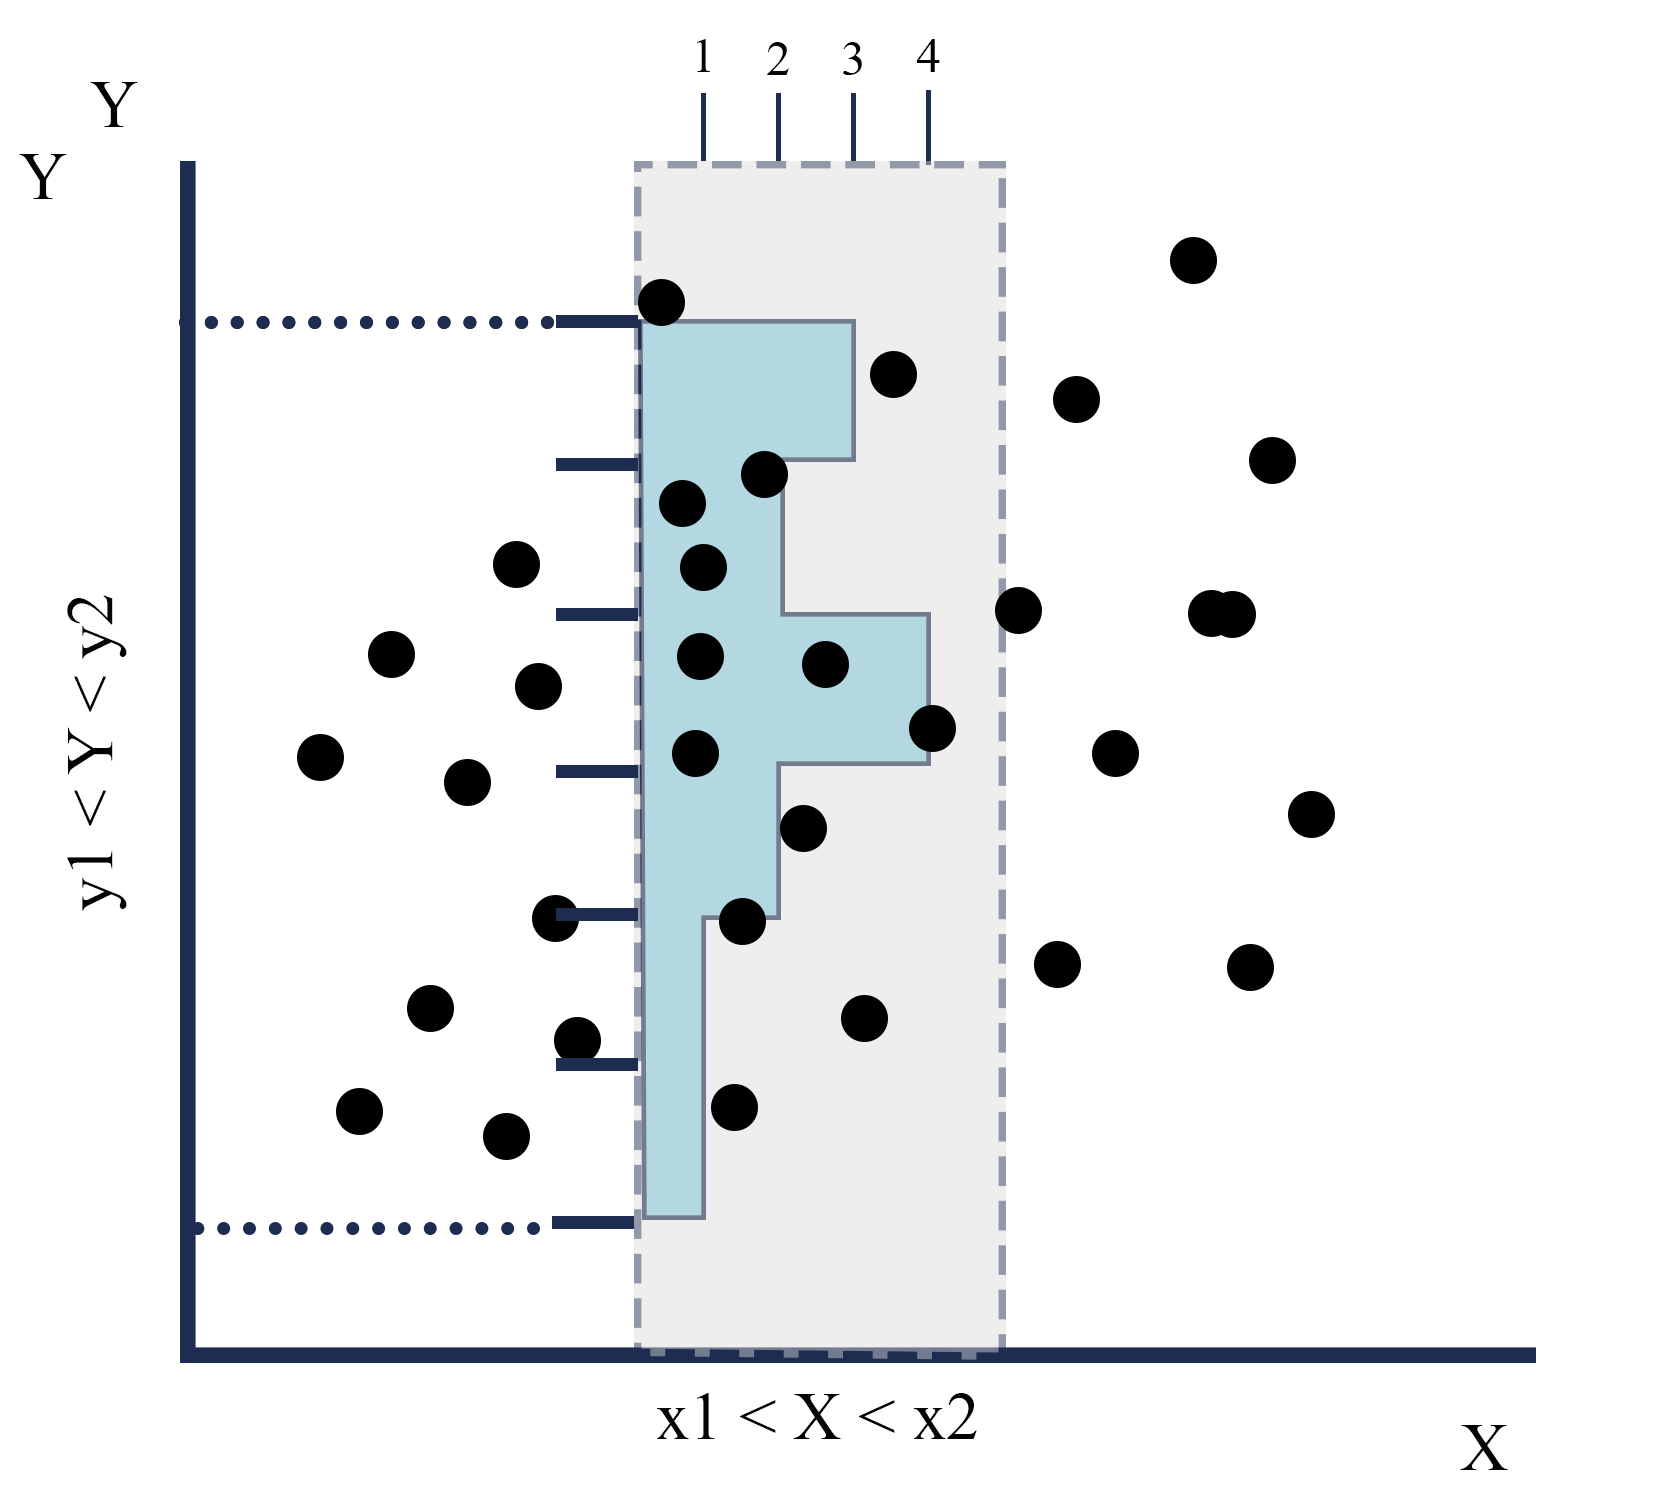
\includegraphics[scale=0.8]{./Capitulo_3/hist_cond.png}	
	\caption{Demonstração do histograma condicional considerando um intervalo de $x_{1}<X<x_{2}$ e $y_{1}<Y<y_{2}$. Podemos considerar  }
	\label{histcond}
\end{figure} 
\FloatBarrier

\section{Ferramentas gráficas}

\subsection{Gráfico Q-Q plot}

O gráfico q-q plot é uma ferramenta para uma primeira análise de diferentes distribuições de variáveis aleatórias. Para cada par conjugado são plotados os quantis de uma variável juntamente com outra. Variáveis que possuam distribuição semelhante tendem a apresentar um comportamento segundo uma reta $y=x$, de inclinação $45^{\circ}$. 

Quando as variáveis apresentam a mesma forma, mas deslocamentos diferentes, ou seja, médias diferenciadas, o gráfico q-q plot apresenta o mesmo formato de uma reta, mas um deslocamento em sua abcissa. Quando as distribuições possuem formas semelhantes, mas variâncias diferentes, a distribuição tende a ter uma inclinação diferente. No entanto, quando distribuições possuem assimetrias e formas diferentes, o gráfico q-q plot tende a produzir uma convexidade diferente. A Figura \ref{QQplot} demonstra o gráfico q-q plot das variáveis Cobalto e Cádmio.

\FloatBarrier
\begin{figure}[!htb]
	\centering
	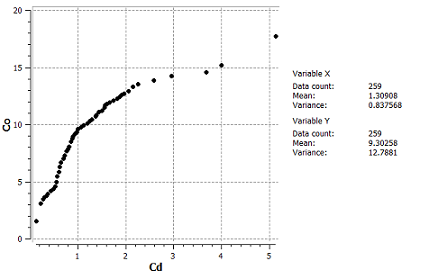
\includegraphics[width=\textwidth]{./Capitulo_3/qq-plot.png}	
	\caption{Gráfico QQ-Plot de Cobalto e Cádmio. Nota-se uma curvatura característica demonstrando pequena correspondência entre as duas populações. Cada ponto representa o mesmo quantil para cada variável }
	\label{QQplot}
\end{figure}
\FloatBarrier

Nota-se na figura que o formato do q-q plot é convexo, demonstrando que as distribuições de dados seguem leis diferenciadas. A figura \ref{histograms} demonstra a comparação entre os histogramas. 

\FloatBarrier
\begin{figure}[!htb]
	\centering
	\includegraphics[width=\textwidth]{./Capitulo_3/histograms.png}	
	\caption{Diferenças entre os histogramas de Cádmio e Cobalto}
	\label{histograms}
\end{figure}
\FloatBarrier

\begin{proposition}
	\textit{O gráfico q-q plot é uma alternativa para comparar distribuições de variáveis diferentes. A utilização da ferramenta, deve ser no entanto, utilizada com sabedoria. Valores outliers podem prejudicar a comparação entre as distribuições, o que não significa que possam ser identificadas como possíveis distribuições semelhantes.}
\end{proposition}

Gráficos q-q plot podem ser utilizados não apenas entre amostras, mas também com uma combinação de uma variável amostrada e os quantis teóricos de uma distribuição. Uma das formas de se averiguar a normalidade de uma distribuição é comparar as amostras padronizadas $Z_{pad} = (Z - \bar{x})/S$ com uma variável gaussiana padrão $\phi(0,1)$. A figura \ref{QQplot_adjust} demonstra 

\FloatBarrier
\begin{figure}[!htb]
	\centering
	\includegraphics[scale=0.6]{./Capitulo_3/q_q_fit.png}	
	\caption{Gráfico da utilização do q-q plot para ajuste de uma distribuição. Quantis de uma amostra padronizada comparadas com quantil de uma distribuição gaussiana padrão. A) Mal ajuste. B) Bom ajuste }
	\label{QQplot_adjust}
\end{figure}
\FloatBarrier

\subsection{Gráfico p-p plot}

Semelhante ao gráfico q-q plot temos o gráfico p-p plot. O gráfico de probabilidades implica nos pares conjugados que indicam a mesma probabilidade $\left(Pr(Z<z),Pr(Y<z)\right) \forall z \in Z,Y $. A figura \ref{ppplot} demonstra o gráfico da variável Cobre pela de Cromo. 

\FloatBarrier
\begin{figure}[!htb]
	\centering
	\includegraphics[width=\textwidth]{./Capitulo_3/pp-plot.png}	
	\caption{Gráfico PP-Plot de Cobre e Cromo. Nota-se uma curvatura característica demonstrando pouca correspondência entre as duas populações. Cada ponto representa o percentual acumulado para o mesmo valor da variável aleatória }
	\label{ppplot}
\end{figure} 
\FloatBarrier

Podemos notar que as diferenças demonstradas no gráfico p-p plot se reproduzem nas diferenças entre os hitogramas de cobre e cromo na figura \ref{histograms2}

\FloatBarrier
\begin{figure}[!htb]
	\centering
	\includegraphics[width=\textwidth]{./Capitulo_3/histograms2.png}	
	\caption{Diferenças entre os histogramas de Cobre e Cromo}
	\label{histograms2}
\end{figure}
\FloatBarrier

A análise do gráfico é feita de forma semelhante ao QQ-plot, no entanto, este gráfico é muito mais sensível à mudança de escala das variáveis. Ele é mais vantajoso quando a ordem de grandeza das variáveis analisadas for semelhante. Neste caso estamos comparando a relação de percentuais acumulados diferentes para o mesmo valor da variável aleatória. 

\subsection{Gráfico de dispersão}
  
O gráfico de dispersão apresenta dados de duas variáveis dispostos nos eixos cartesianos. Temos uma variável \textbf{preditora} (X) e uma variável \textbf{resposta} (Y). Os pares conjugados $(x_{i}, y_{i}) \in X,Y$ representam pontos em um plano cartesiano.

\begin{proposition}
	\textit{Uma das primeiras utilizações da regressão linear foi no estudo da importância de tendências entre gerações. Durante o período de 1893-1898, E. S. Pearson organizou uma coleção de n=1375 alturas de mães do reino Unido abaixo de 65 anos e uma de suas filhas acima de 18. O interesse era computar o tamanho das mães (Mheight) com o tamanho das filhas (Dheight) como preditor. Se todas as mães possuirem tamanho igual suas filhas, os dados estarão dispostos em uma reta de inclinação $45^{circ}$. A linearidade proposta pela dispersão identifica que mães mais altas geralmente possuem filhas mais altas.} - \cite{weisberg2005applied}
\end{proposition}

Para a utilização do gráfico os dados devem estar colocados. Isso significa que a amostra 1 deve ter a mesma origem da amostra 2, ou o mesmo suporte. Logo só podemos realizar um gráfico de dispersão com vetores de amostras do mesmo tamanho. 

Caso a amostragem apresente dados inválidos para uma variável devemos utilizar um filtro para separar apenas os dados colocados. Existem técnicas estatísticas que permitem o tratamento de dados perdidos ou inexistentes, mas nada substitui a amostra em termos de informação sobre o objeto de estudo. A figura \eqref{scatter} demonstra um gráfico de dispersão entre a variável cromo e cobalto.
  
\begin{figure}[H]
  	\centering
  	\includegraphics[width=\textwidth]{./Capitulo_3/scatter.png}	
  	\caption{Gráfico de dispersão da variável Cromo e Cobalto. Nota-se dependência linear positiva entre as variáveis. }
  	\label{scatter}
\end{figure} 
   
Nota-se pela figura que as variáveis possuem \textbf{dependência linear positiva} entre a variável Cromo e Cobalto. Isso significa que amostras com valor grande de cromo podem apresentar valores grandes de cobalto. O contrário também pode acontecer, alguns minerais como quartzo e piroxênio são inversamente proporcionais em rochas magmáticas. À medida em que se aumenta o teor de quartzo tende-se a reduzir o teor de piroxênio na amostra de rocha. Neste caso possuímos uma \textbf{dependência linear negativa} 

A Figura \ref{correlacao_linear} demonstra os tipos de correlação lineares possíveis. Em \ref{correlacao_linear} -a temos a correlação linear positiva em que o aumento da variável X aumenta o valor de Y, em \ref{correlacao_linear} -b temos a correlação linear negativa em que o aumento do valor X tende a diminuir o valor de Y e em \ref{correlacao_linear} -c temos um caso de independência entre as variáveis, tal que o aumento da variável X não altera o valor da variável Y. 

\begin{figure}[H]
	\centering
	\includegraphics[width=\textwidth]{./Capitulo_3/correlacao_linha.png}	
	\caption{Figura demonstrando os tipos de correlação linear possíveis. A) Correlação linear positiva, B) Correlação linear negativa, C) Sem correlação }
	\label{correlacao_linear}
\end{figure}



Os gráficos de dispersão também são uma boa medida para a visualização de valores outliers. A figura \eqref{scatter_out} demonstra a dispersão anterior mas com uma área circulada de pontos que não estão dentro do comportamento linear das variáveis. Neste caso para valores intermediários de Cobalto temos grandes valores de Cromo.

 \begin{figure}[H]
 	\centering
 	\includegraphics[width=\textwidth]{./Capitulo_3/scatter_out.png}	
 	\caption{Gráfico de dispersão da variável Cromo e Cobalto demonstrando valores outliers. Círculo vermelho indica possíveis valores fora dos padrões das variáveis conjuntas }
 	\label{scatter_out}
 \end{figure} 
 
 Muitas vezes um valor outlier em um gráfico bivariado não é demonstrado no tratamento individual das amostras. Muito cuidado deve ser tomado para a retirada de pares anômalos das estatísticas, pois eles podem gerar novos valores discrepantes e não demonstrarem um padrão de maior correlação entre as variáveis.
 
     
  \section{Regressão linear }
  
  O modelo de regressão linear simples é aquele em que definimos uma dependência diretamente proporcional entre a variável resposta Y e preditora X. Podemos associar o valor esperado da variável resposta dado valores da variável preditora tal que $E(Y|X=x) = \beta_{0} + \beta_{1}x$. Note que $E(Y|X=x)$ corresponde ao \textbf{valor médio da variável Y condicionado a um valor x da variável X}, e $\beta_{0}$ e $\beta_{1}$, também são o \textbf{intercepto da reta no eixo das abcissas} e \textbf{a tangente do ângulo de inclinação da reta}  . Muitas pessoas acabam por não entender que a regressão linear pode não apresentar uma representação acurada da resposta dado um valor da variável preditora, porque o valor estimado pela regressão não é o valor da variável resposta, mas sim seu valor esperado condicionado. Muitas variáveis apresentam alta dispersão em torno de seus valores médios e podem não ser estimativas plausíveis. a solução da \textbf{regressão linear ordinária} geralmente advém do método dos mínimos quadrados. Considere $\hat{y}_{i}=\hat{E}(Y|X=x)$ como um estimador para $E(Y|X=x)$, logo teremos que o resíduo pode ser demonstrado pela equação  $\hat{y}_{i}-y_{i}$ segundo a equação   
 
 \FloatBarrier 
 \begin{proof}
  	Regressão linear pelo método dos mínimos quadrados
  	\begin{align*}
  	&\epsilon_{i} =  \hat{y}_{i}-y_{i}  \\
  	&\epsilon_{i}^{2} = \hat{y}_{i}^{2} + y_{i}^{2} - 2\hat{y}_{i}y_{i}\\
  	&\epsilon_{i}^{2} = (\hat{\beta_{0}} + \hat{\beta_{1}}x_{i})^{2} + y_{i}^{2} - 2(\hat{\beta_{0}} + \hat{\beta_{1}}x_{i})y_{i}\\
  	&\text{A soma dos erros quadraticos para cada i} \\
  	&\sum_{i=0}^{n}\epsilon_{i}^{2} = \sum_{i=0}^{n}(\hat{\beta_{0}} + \hat{\beta_{1}}x_{i})^{2} + \sum_{i=0}^{n}y_{i}^{2} - \sum_{i=0}^{n}2(\hat{\beta_{0}} + \hat{\beta_{1}}x_{i})y_{i}\\
  	&\text{Tomando as derivadas parciais segundo os parâmetros: } \hat{\beta_{0}},\hat{\beta_{1}}\\
  	&1)\frac{\partial \sum_{i=0}^{n}\epsilon_{i}^{2}}{\partial \hat{\beta_{0}}} = 2\hat{\beta_{0}}n + 2\hat{\beta_{1}}\sum_{i=0}^{n}x_{i} - \sum_{i=0}^{n}2y_{i} = 0 \\
  	&2)\frac{\partial \sum_{i=0}^{n}\epsilon_{i}^{2}}{\partial \hat{\beta_{1}}} = 2\hat{\beta_{1}}\sum_{i=0}^{n}x_{i}^{2} + 2\sum_{i=0}^{n}\hat{\beta_{0}}x_{i} - 2\sum_{i=0}^{n}y_{i}x_{i} =0 \\
  	\end{align*}
  \end{proof}
 \FloatBarrier 
 
 
A obtenção dos parâmetros pode ser facilmente encontrada isolando os termos das equações 1 e 2. Podemos então determinar 

 \FloatBarrier 
\begin{proof}
 	Obtenção dos parâmetros da regressão
 	\begin{align*}
  	&\hat{\beta_{0}} = (\sum_{i=0}^{n}y_{i} - \hat{\beta_{1}}\sum_{i=0}^{n}x_{i})/n \\
  	&\text{Substituindo em 2}\\
  	&\hat{\beta_{1}}\sum_{i=0}^{n}x_{i}^{2} + \sum_{i=0}^{n}(\sum_{j=0}^{n}y_{j} - \hat{\beta_{1}}\sum_{j=0}^{n}x_{j})x_{i}/n - \sum_{i=0}^{n}y_{i}x_{i} =0 \\
  	&\hat{\beta_{1}}\sum_{i=0}^{n}x_{i}^{2} - \hat{\beta_{1}}\bar{x}\sum_{i=0}^{n}x_{i} + \bar{x}\sum_{i=0}^{n}y_{i} - \sum_{i=0}^{n}y_{i}x_{i} = 0  \\
  	&\hat{\beta_{1}}(\sum_{i=0}^{n}x_{i}^{2} - \bar{x}\sum_{j=0}^{n}x_{i}) = \sum_{i=0}^{n}y_{i}x_{i} - \sum_{j=0}^{n}y_{j}\bar{x}\\
  	&\hat{\beta_{1}} = \frac{\sum_{i=0}^{n}y_{i}x_{i} - \sum_{j=0}^{n}y_{j}\bar{x}}{\sum_{i=0}^{n}x_{i}^{2} - \bar{x}\sum_{j=0}^{n}x_{i}}\\
    \end{align*}
\end{proof}
 \FloatBarrier 
 
    
  O problema de regressão linear se torna então um problema de otimização ao encontrar o menor somatório dos desvios quadrádicos. A figura \eqref{scatter_expl} demonstra graficamente o problema da regressão linear. Neste caso os valores dos coeficientes lineares das retas podem ser encontrados a partir de derivação simples ou por meio de métodos numéricos, como a utilização do \textbf{método Simplex}. O resultado também é análogo ao \textbf{método de máxima verossimilhança} considerando a distribuição dos resíduos como gaussianos. 
  
\FloatBarrier  
\begin{figure}[!htbp]
  	\centering
  	\includegraphics[scale=0.5]{./Capitulo_3/regress_expl.png}	
  	\caption{Explicação da regressão linear entre a variável independente X e a variável dependente Y. Barras verticais representando o os desvios das amostras com o valor médio. }
  	\label{scatter_expl}
\end{figure}
\FloatBarrier  

Como a regressão linear assume a minimização dos valores quadráticos, os parâmetros e $\beta_{0}$ e $\beta_{1}$ podem ser fortemente afetados por valores outliers. As propostas mais modernas de regressão prevem que a regressão seja utilizada apenas em parte dos dados, e avaliada com outra quantidade dos dados. Os dados utilizados para a estimativa dos parâmetros é chamada de  Assim conseguimos avaliar a qualidade da predição de acordo com a dispersão destes resíduos. 

\FloatBarrier
\begin{figure}[!htbp]
	\centering
	\includegraphics[scale=0.8]{./Capitulo_3/graf_resd.png}	
	\caption{Gráfico da dispersão de resíduos nos bancos de dados de treino e teste. Dados de treino utilizados para determinar os parâmetros da regressão e dados de teste para avaliar as diferenças do modelo de predição }
	\label{scatter_expl}
\end{figure}
\FloatBarrier
   
Na geoestatística utilizamos estimadores lineares, semelhantes ao processo de regressão linear. É observado que para aplicações na mineração  que utilizem os métodos geoestatísitcos clássicos, o erro do valor estimado é ligeiramente diferente de uma distribuição gaussiana, para problemas lineares e estacionários. Temos uma maior confiabilidade do valor esperado estimado utilizando krigagem ordinária do que utilizando regressão linear ordinária. Na verdade, o método de regressão linear ordinária é pouco usual nos dias atuais, considerando os diferentes modelos possíveis e robustos (menos influenciados pelos valores outliers), no entanto, ainda é um método muito popular pela sua simplicidade e facilidade de aplicação.

\begin{remark}
	\textit{Em aplicações da mineração, a distribuição dos erros da função aleatória são geralmente simétricos com um crescimento mais pronunciado na moda e caudas alongadas do que para distribuições normais com mesma média e variância. Então em relação a uma distribuição normal, há menos erros na região próxima ao valor esimado e mais erros nas caudas.} - \cite{journel1978mining}
\end{remark}
 
 \section{Intervalo de segurança para a regressão linear}
 
 A determinação do modelo de regressão consiste em estimar parâmetros $\beta_{0}$ e $\beta_{1}$ para econtrarmos o valor estimado $\hat{y}_{i} = E(Y|X=x_{i})$. No entanto, se a nuvem de pontos determinada pela regressão for esparsa, o valor $\hat{y}_{i}$ não possui capacidade preditiva e pode encontrar-se dentro de limites amplos. Considerando que a distribuição dos resíduos seja normalmente distribuída, podemos encontrar os limites da regressão para bandas superiores e inferiores, determinando assim a confiabilidade desta reta regredida.  A equação \eqref{intervalo_seguranca} demonstra como podem ser calculadas as bandas de incerteza da regressão de acordo com um nível de significância estipulado. 
 
 \begin{equation}\label{intervalo_seguranca}
	 \hat{y}_{i} \pm  t^{*}_{(n-2,p)} s_{y} \sqrt{\frac{1}{n}+\frac{(x_{i}-\bar{x})^2}{(n-1)s^2_{x}}}
 \end{equation}
 
 Em que $x_{i}$ é o valor da variável X, $t^*$ é o valor da distribuição de t-student para um grau de liberdade igual a $n-2$ e nível de significância p, enquanto $s_{y}$ pode ser demonstrado segundo a equação \eqref{intervalo_seguranca2}
 
  \begin{equation}\label{intervalo_seguranca2}
  s_{y} = \sqrt{\frac{\sum_{i}(y_{i}-\hat{y}_{i})^2}{n-2}}
  \end{equation}
   
  Em que $y_{i}$ é o valor da coordenada y para um ponto amostral i. Ou seja $s_{y}$ é o valor do desvio padrão entre os valores amostrais e os valores médios estimados pela regressão. 
  
  A figura \eqref{inter_seg} demonstra o intervalo de segurança para o valor regredido. 
  
  \begin{figure}[H]
  	\centering
  	\includegraphics[scale=0.8]{./Capitulo_3/banda_incerteza.png}	
  	\caption{Demonstração do intervalo de confiança para a regressão linear. Banda de incerteza adicionada como limite inferior e superior dado pela equação \eqref{intervalo_seguranca} }
  	\label{inter_seg}
  \end{figure}
  
  Nota-se que as bandas apesar de acompanharem o valor de regressão linear não são retas, apresentado um maior estreitamento na região mediana da dispersão. A confiabilidade do centro de dispersão da reta regredida é sempre maior. 
  
 \begin{proposition}
 \textit{Os intervalos de confiança para a regressão linear estipulam que os resíduos seguem uma distribuição gaussiana. Isto porém, pode não se apresentar na prática. A única garantia que temos para que este resíduo seja considerado gaussiano, é se por ventura, a distribuição dos dados segue uma lei de probabilidades \textbf{multigaussiana}. Este é o pressuposto de técnicas mais avançadas de geoestatística não-linear. As bandas de incerteza devem ser consideradas como uma alternativa para verificar dados discrepantes, mas não como uma métrica de decisão na detecção de valores outliers.} 
 
\end{proposition}
  

  
 \section{Regressão linear múltipla}
 
 Quando pensamos em apenas uma variável preditora, a determinação de $\hat{y}_{i}$ se limita a encontrar o valor de $E(Y|X=x_{i})$. Porém quando múltiplas variáveis são relacionadas o problema se torna encontrar $E(Y|X^{1}=x^{1}_{i},X^{2}=x^{2}_{i},...,X^{n}=x^{n}_{i})$. O modelo de regressão linear múltipla é um caso extendido da regressão linear simples para múltiplas variáveis. Neste caso temos um conjunto de n variáveis preditoras e uma variável resposta
 
  \begin{equation}\label{eq1:Metodo_dos_minimos_quad}
  \hat{y}_{i} = \hat{\beta_{0}} + \hat{\beta_{1}} x^{1}_{i} + \hat{\beta_{2}} x^{2}_{i} + ... + \hat{\beta_{n}} x^{4}_{i} = \sum_{j=0}^{p} \hat{\beta_{j}} x^{j}_{i}
  \end{equation} 
  

  
  Onde $x^{0}_{i}$ é sempre igual a 1 para $j$ variáveis de 0 a p. O problema se resume a encontrar $\hat{\beta_{p}}$ parâmetros que aproximem melhor a combinação dos valores das variáveis $x^{p}_{i}$ de $\hat{y}_{i}$. Podemos definir o problema de regressão linear múltipla a partir de sua forma matricial pela equação \eqref{matricial}
  
  \begin{equation}\label{matricial}
  \begin{pmatrix}
  y_{1}\\ 
  y_{2}\\
  \vdots\\
  y_{n}
  \end{pmatrix}=\begin{pmatrix}
  1      & x^{1}_{1} & \cdots & x^{p}_{1}\\ 
  1      & x^{1}_{2} & \cdots & x^{p}_{2}\\ 
  \vdots & \vdots    & \vdots & \vdots \\ 
  1      & x^{1}_{n} & \cdots & x^{p}_{n}
  \end{pmatrix}\begin{pmatrix}
  \beta_{0}\\ 
  \beta_{1}\\
  \vdots\\
  \beta_{n}
  \end{pmatrix}
  \end{equation} 
  
  Ou de forma simplificada pela equação \eqref{matricial2}
  \begin{equation}\label{matricial2}
  	\bar{Y} = \bar{X}\bar{\beta}
  \end{equation}
  
  Onde $\bar{Y}$ representa o vetor da variável resposta, $\bar{X}$ a matriz das variáveis preditoras e $\bar{\beta}$ os parâmetros. A obtenção dos parâmetros a partir da regressão mútlipla pode ser facilmente encontrado através de operações matriciais.
  
 \FloatBarrier 
\begin{proof}
	Obtenção dos parâmetros da regressão
	\begin{align*}
	&\bar{Y} = \bar{X}\bar{\beta} \\
	&\bar{X}\bar{Y} = \bar{X}\bar{X}\bar{\beta} \\
	&(\bar{X}\bar{X})^{-1}\bar{X}\bar{Y} = \bar{\beta}\\
	&(\bar{X}\bar{X})^{-1}\bar{X}\bar{Y} = \bar{\beta}\\
	&X^{\dagger}\bar{Y}= \bar{\beta}\\
	&\text{tal que :} X^{\dagger} = (\bar{X}\bar{X})^{-1}X \\ 
	\end{align*}
\end{proof}
\FloatBarrier 
  
Em que $X^{\dagger}$ também é chamada de pseudo-inversa de X. Se no caso da regressão ordinária simples obtínhamos um valor regredido a partir da minimização do resíduo de uma variável, neste momento obtemos o resíduo a partir de uma combinação de múltiplas variáveis. O erro quadrático pode ser obtido a partir da equação \eqref{erroquad}. 
  
 
 \begin{equation}\label{erroquad}
 \sum_{i} \epsilon_{i}^2 = \sum_{i} \left( y_{i} - \sum_{j=0}^{p} \hat{\beta_{j}} x^{j}_{i} \right)^{2}
 \end{equation}
 
A obtenção dos parâmetros $\beta_{p}$ pode ser calculado a partir das técnicas de minimização dos resíduos, formando um sistema de $p$ derivadas parciais Um dos grandes problemas da regressão linear múltipla é o fato de que as grandezas de variáveis diversas podem ser diferentes e impactar de forma diferenciada nos pesos da regressão.Esse problema de dimensão geralmente pode ser minimizado se padronizarmos as variávies como visto no capítulo \ref{est_univ}. Outra questão envolvendo a regressão múltipla é o fato de que valores outliers conseguem ser ainda mais prejudiciais que a regressão linear ordinária, afetando muito a estimativa dos pesos. Uma tentativa de excluir certos efeitos de valores discrepantes é introduzir uma constante adicional chamada de \textbf{regularização} ($\lambda$) multiplicando os valores dos parâmetros $\beta_{p}$. 
  
  \section{Coeficiente de correlação }
  
  Observamos na seção anterior que se duas variáveis são dependentes, podemos assumir que existe uma probabilidade $P(Y|X=x)$. No entanto, as probabilidades condicionais parecem não fornecer um quadro geral da dependência de uma variável aleatória $Y$, pois precisamos saber qual valor a variável $X$ deve assumir. É necessário ter uma métrica para avaliarmos o quão forte ou fraca é a dependência entre as variáveis. Imagine o caso onde temos um depósito hidrotermal de ouro, associado principalmente a rochas magmáticas sulfetadas. Se existir uma alta dependência do conteúdo de ouro com o de enxofre, podemos assumir que o conhecimento de uma variável auxiliará no conhecimento da outra. Porém valores pequenos de teor de enxofre podem ser menos dependentes do teor de ouro do que para altos valores do teor de enxofre. Esta discrepância dado alguns limites pode ser favorável para o uso de probabilidades condicionais nas caudas da distribuição de enxofre, mas não garante uma visão geral da dependência linear entre estas variáveis. 
  
  \begin{remark}
  	\textit{Tanto na natureza como em vários problemas de engenharia nos deparamos com a dependência entre diferentes variáveis. Em muitos casos estas dependências podem ser modeladas linearmente. Em outros casos, quando conhecemos propriedades físicas relacionáveis, podemos utilizar \textbf{transformações lineares}, capazes de transformar modelos não lineares em lineares.} 
  \end{remark}

No capítulo \ref{cap_var_reg} observamos a correlação como uma medida de dependência entre variáveis aleatórias. A covariância teórica pode ser estimada a partir de sua covariância experimental pela equação \eqref{correst} 

\begin{equation}\label{correst}
\hat{Cov}_{X,Y} = \frac{\sum_{i=0}^{n} (x_{i} - \bar{x})(y_{i} - \bar{y})}{n}
\end{equation}

Onde $\bar{x}$ e $\bar{y}$ são as médias aritméticas entre as variáveis X e Y para um número de amostras n. A covariância experimental pode ser muito bem comparada ao produto escalar obtido pela multiplicação de dois vetores $X*Y = \left \| X\right \| \left \| Y  \right \| cos(\theta)$, em que $cos(\theta)$ é chamado de cosseno diretor da projeção de $X$ em $Y$. Quando a projeção do vetor $X$ corresponde ao vetor $Y$ temos o máximo valor possível, no entanto, quando estes vetores são perpendiculares temos um valor de $cos(90^{\circ})=0$, e portanto $\hat{Cov}_{X,Y} =0$  

A covariância é uma medida muito susceptível a valores outliers, pois como X e Y podem ter unidades discrepantes, o produto das duas pode ser mais influenciado por aquela variável que apresentar maiores valores. Imagine que procuremos a relação entre a massa em quilos dos testemunhos e o teor de um elemento químico. Como a massa dos testemunhos poderá variar de valores acima da unidade, como por exemplo 12kg e os teores apenas com valores decimais, como 0.12, a importância dada para as variações do peso serão maiores. Isto torna a a covariância pouco comparativa, apenas se considerarmos a normalização das variáveis. A alternativa para isto é normalizarmos a covariância pelos desvios padrões das respectivas variáveis, o que gera o \textbf{coeficiente de correlação de Pearson} \eqref{rozinho}.   


\begin{equation}\label{rozinho}
\rho_{X,Y}^{p} = \frac{\sum_{i=0}^{n} (x_{i} - \bar{x})(y_{i} - \bar{y})}{\sqrt{\sum_{i=0}^{n}(x_{i} - \bar{x})^{2}(y_{i} - \bar{y})^{2})}} 
\end{equation}
 
 Os valores de $\rho_{X,Y}$ podem variar de -1 a 1, sendo 1 quando apresenta correlação positiva perfeita e -1 quando apresenta correlação negativa perfeita. Quando $\rho_{X,Y}^{p} = 0$ temos um indicativo de independência entre as variáveis tal que $\hat{Cov}_{X,Y}$ é igual a 0. Podemos obter a relação entre o coeficiente de Pearson e a correlação pela equação \eqref{rozinho2}
 
 \begin{equation}\label{rozinho2}
 \rho_{X,Y}^{p} = \frac{\hat{Cov}_{X,Y}}{\sqrt{S_{x}^{2} S_{y}^{2}}} 
 \end{equation}
 
 Onde $\hat{Cov}_{X,Y}$ representa a covariância estimada, e $S_{x}^{2}$ e $S_{y}^{2}$ as variâncias experimentais das amostras x e y. Para que consigamos calcular o valor do coeficiente de variação e da correlação, precisamos que existam valores correspondentes tanto para as amostras x e y, ou seja, precisamos de dados \textbf{colocados}. Se por ventura houverem dados faltantes, não consiguiremos calcular a covariância ou o coeficiente de correlação. 
 
 Em alguns casos não desejamos observar a dependência entre os valores da variável, mas precisamos saber qual é a dependência da \textbf{ordem} dos dados. Para isto realizamos uma medida chamada de \textbf{rank ou posto}, que representa a ordem de uma amostra em seu conjunto. 
 
\begin{definition} [Rank ou posto]
	\textit{Um rank ou posto é a ordem crescente de uma amostra em seu respectivo conjunto. Por exemplo, um conjunto de amostras com valores $x={3,41,2,57,8,9,6}$, possuirá um rank $R_{x}$ tal qual $R_{x} = {2,6,1,7,4,5,3}$ }
\end{definition}
 
O chamado \textbf{coeficiente de correlação de Spearman} nada mais é que a correlação de Pearson considerando seus respectivos postos. 

 \begin{equation}\label{Spearman}
\rho_{X,Y}^{s} = \frac{\hat{Cov}_{R_{x},R_{y}}}{\sqrt{S_{R_{x}}^{2} S_{R_{y}}^{2}}} 
\end{equation}	 

Enquanto a correlação de Pearson é uma medida linear de dependência, o coeficiente de Spearman é uma medida não linear, demonstrando a correlação entre crescimentos e descrescimentos das variáveis independente dos valores dos dados. Uma função parabólica tal que $Y = \beta_{1} X^{2}  + \beta_{0} $ apresentará um valor de coeficiente de correlação de Pearson muito baixo, porém um valor de Coeficiente de Spearman igual a 1. 
\section{Exercícios}

\begin{exercise}
	
	Os dados da tabela abaixo representam valores de Au e cobre medidos concumitamente nos mesmos testemunhos de sondagem. Com estes dados, pede-se:
	
	a) Determine a covariância dos dados 
	
	b) Determine o coeficiente de correlação.
	
	c) As amostras são dependentes positivamente ou negativamente?
	
	d) Faça um gráfico de regressão linear entre as variáveis ouro e cobre
	
	\begin{tabular}{lllll}
		\hline
		Au & Cobre &  &  &  \\ \hline
		0.012      & 2.0  &  &  &  \\
		0.015      & 2.02 &  &  &  \\
		0.013      & 1.32 &  &  &  \\
		0.070      & 3.45 &  &  &  \\
		0.012      & 1.02 &  &  &  \\
		0.067      & 2.19 &  &  &  \\
		0.090      & 4.01 &  &  &  \\
		0.08      & 3.67 &  &  &  \\
		0.012      & 1.43 &  &  &  \\
		0.011      & 1.01 &  &  &  \\
		0.011      & 1.05 &  &  &  \\ \hline
	\end{tabular}
\end{exercise}

\begin{exercise}
	
	Os dados da tabela abaixo representam valores de X e Y. Faça um gráfico de dispersão e determine o par de valor outilier para o gráfico.
	
	\begin{tabular}{lllll}
		\hline
		X & Y &  &  &  \\ \hline
		0.729      & 1.546&  &  &  \\
		0.757      & 1.683&  &  &  \\
		0.140      & 0.175 &  &  &  \\
		0.575      & 0.963 &  &  &  \\
		0.408      & 0.726 &  &  &  \\
		0.402      & 1.104 &  &  &  \\
		0.616      & 1.321 &  &  &  \\
		0.958      & 5.02 &  &  &  \\
		0.9136      & 1.873 &  &  &  \\
		0.527      & 0.853 &  &  &  \\
		0.470      & 0.960 &  &  &  \\ \hline
	\end{tabular}
\end{exercise}
\chapter{Métodos clássicos e desagrupamento} \label{Cap_4}

\begin{myquoting}{G.Matheron}
	
	Difficultés rencontrées dans le développement d'une Géostatistique linéaire. A cette émergence lente et difficile, nous apercevons plusieurs sortes de raison, les unes historiques, d'autres simplement psychologiques, et d'autres encore qui correspondent a des problèmes de fond, à de véritables difficultés méthodologiques, ou épistémologiques qui n'ont été vraiment élucidées qu'à la fin des années 60 ou au début des années 70
\end{myquoting}

\section{Introdução} 

Apesar de antiga, a geoestatística se iniciou como um alternativa para tentativas de avaliação de depósitos minerais antes da década de 70. Os métodos chamados de clássicos eram relativamente eficientes para condições de depósitos minerais mais homogêneos e de classificação estatística dentro dos grupos considerados regulares. No entanto, devido a intensa atividade industrial humana, é necessário aproveitarmos cada vez mais depósitos minerais complexos. Diferentemente dos métodos geoestatísticos, os métodos convencionais baseiam-se apenas na distribuição geométrica entre as amostras e não na correlação e dependência entre variáveis aleatórias. Apesar de ultrapassados, os métodos de avaliação clássica ainda são utilizados em depósitos de baixa variabilidade e com quantidades de amostras muito baixas, como por exemplo, depósitos estratiformes de argila ou areia. Em alguns casos bem específicos os métodos clássicos podem até mesmo apresentar resultados superiores aos métodos geoestatísticos seguindo o princípio da navalha de Occan. 

\begin{definition}[Navalha de Occan]
	\textit{"A navalha de Occam é um princípio lógico atribuído ao filósofo medieval William de Occan. O princípio estabelece que não se deve assumir mais suposições do que necessário. Também é chamado de princípio da parsimônia. Este princípio envolve todo a modelagem científica e construção de teorias. Ele nos incentiva a escolher de um grupo de modelos equivalentes para um dado fenômeno aquele mais simples. Para todo modelo, a nvalha de Occan nos ajuda a 'cortar' aqueles conceitos, variáveis ou construções que não conseguem realmente explicar o fenômeno. Ao fazer isso, o desenvolvimento do modelo se torna bem mais simples, e há menos chances de introduzir inconsistências, ambiguidades ou redundâncias"} -\cite{heylighen1997occam} 

\end{definition} 

  Veja bem que adotar os métodos clássicos em detrimento da geoestatística utilizando a navalha de Occan só possui bons resultados em dois casos. No primeiro o problema é tão simples e o depósito mineral tão homogêneo  e pouco amostrado, que se torna factível o uso de um modelo extremamente simplificado. No segundo caso temos um problema tão complexo e variável que se torna impossível encontrar aparentemente um padrão qualquer no fenômeno, sendo mais fácil adotar valores médios pela distância do que realmente utilizar um método geoestatístico refinado.  Segundo o professor \cite{yamamoto2001avaliaccao} , os métodos chamados de clássicos baseiam-se no princípio da \textbf{interpretação}, aos quais determinam valores a partir de duas amostras contíguas. É possível a partir da disposição das amostras encontrar valores estimados. Estes princípios segundo o professor são: 
  
  \begin{enumerate}
  	\item Mudança gradual ou lei de função linear 
  	\item Pontos mais próximos ou esfera de igual influência 
  	\item Generalização ou empírico
  \end{enumerate}
 
\subsection{Princípio da mudança gradual} 

O princípio da mudança gradual indica que uma mudança de uma propriedade acontece de forma contínua de uma amostra pontual $P1$ até uma amostra pontual $P2$. Pelo princípio da navalha de Occan, a função utilizada para realizar esta transição geralmente é uma variação linear. Dada uma propriedade como o teor $T$ a ser estimada a partir das propriedades $T1$ e $T2$ de dois pontos amostrais no espaço, com respectivas distâncias $D1$ e $D2$ da origem, realizamos a interpolação deste valor a partir de sua distância $D$ entre os pontos pela equação \eqref{difgrad}.

\begin{equation}\label{difgrad}
	T=T_{1}+ \frac{(D-D_{1})(T_{2}- T_{1})}{(D_{2} - D_{1})}
\end{equation}

A figura \ref{mudgrad} apresenta o resultado geométrico  da interpolação linear realizada entre os pontos amostrais. 

\FloatBarrier
\begin{figure}[!htpb]
	\centering
	\includegraphics[scale=0.4]{./Capitulo_4/Gradual.png}	
	\caption{Princípio da mudança gradual de um teor para duas amostras no espaço $P1$ e $P2$, variação linear dos teores para uma distância $D$ considerada.}
	\label{mudgrad}
\end{figure}
\FloatBarrier

\subsection{Princípio dos pontos mais próximos} 

O princípio dos pontos mais próximos assume que o valor interpolado é igual ao valor da amostra mais próxima dele. Este processo também é chamado de \textbf{vizinho mais próximo}. Dado um conjunto de amostras no espaço $P = \{P_{1},P_{2},P_{3},...,P_{n},\}$ com propriedades $T = \{T_{1},T_{2},T_{3},...,T_{n},\}$, com respectivas posições espaciais segundo um eixo cartesiando $(x,y,z)$, o valor de uma propriedade $T_{0}$ para uma amostra $P_{0}$ no espaço assume o valor 

\begin{equation}\label{vizinhoprox}
T_{0} = T_{i} | i \rightarrow min(\| P_{0},P_{i}\|), \forall i\in [1,n]
\end{equation}

Em que $\| P_{0},P_{i}\|$ representa a distância euclidiana entre o par conjugado de pontos no espaço para $n$ amostras, $min()$ representa o mínimo valor. A figura \ref{mindist} apresenta o princípio dos pontos mais próximos. Cinco pontos amostrais são apresentados P1, P2, P3, P4 e P5. Como a distância mínima entre o ponto a ser amostrado P0 até o ponto amostral mais próximo é D2, T0 recebe o valor de T2. 

\FloatBarrier
\begin{figure}[!htpb]
	\centering
	\includegraphics[scale=0.4]{./Capitulo_4/mindist.png}	
	\caption{Princípio dos pontos mais próximos. Conjunto de pontos amostrais P1, P2, P3, P4, P5 para um ponto amostral estimado P0. Como a menor distância euclidiana entre o ponto P0 é o ponto P2, assumimos que a propriedade T0 =T2. }
	\label{mindist}
\end{figure}
\FloatBarrier 

\subsection{Princípio da generalização}

Segundo critérios geológicos é possível realizar a extrapolação de uma dada propriedade segundo a continuidade do depósito mineral. Este princípio é justificado nas fases inciais de pesquisa para ajustar uma dada tendência das propriedades do depósito mineral. A figura \ref{extrap} demonstra a extrapolação do teor a partir do conhecimento de uma falha geológica entre os pontos amostrais $P1$ e $P2$. A partir da atitude da camada é estipulado uma variação segundo os teores extrapolados.

\FloatBarrier
\begin{figure}[!htpb]
	\centering
	\includegraphics[scale=0.4]{./Capitulo_4/extrap.png}	
	\caption{Princípio da generalização e extensão dos teores a partir de um critério geológico. Falha geológica observada entre os pontos amostrais $P1$ e $P2$. Ponto estimado $P0$ é determinado a partir de diferenças entre os teorers e inclinação da camada. }
	\label{extrap}
\end{figure}
\FloatBarrier 

\section{Composição} 

Para realizar a análise geoestatística é necessário prover de amostras com mesmo \textbf{suporte}. Como testemunhos de sondagem podem representar fragmentos de tamanho distintos, é necessário realizar a \textbf{regularização} dos tamanhos das amostras. Isto significa que ao invés de tomarmos as propriedades referentes a apenas os fragmentos dos testemunhos de sondagem (litotipo, teores, propriedades físicas, etc.), tomamos a amostra como um valor de média ponderada entre os diversos tamanhos de fragmentos dos testemunhos. Observe a figura \ref{composicao}. Os framentos do testemunho de sondagem são respectivamente os valores $\{l_{1}, l_{2}, l_{3}, l_{4}\}$. Para consideramos este testemunho de sondagem como medidas representativas para a geoestatística consideramos duas composições de tamanho $\{C_{1}, C_{2}\}$, em que $\{x_{1}, x_{2}\}$ representam as respectivas partes dos fragmentos $\{l_{1}, l_{2}\}$ em $C_{1}$ . Se ${t_{1}, t_{2}, t_{3}, t_{4}}$ são propriedades aditivas como os teores dos fragmentos, podemos encontrar o valor da propriedade da composição $t_{C1}$ pela relação \eqref{eq:composition}

\begin{equation}\label{eq:composition}
t_{C_{1}} = \frac{(x_{1}/l_{1})t_{l_{1}} + (x_{2}/l_{2}) t_{l_{2}}}{(x_{1}/l_{1}) + (x_{2}/l_{2})}
\end{equation}

Em que $(x/l)$ representa a proporção de um dado fragemento dentro da composta. Podemos generalizar o caso da composição para n fragmentos de acordo com a relação \eqref{eq:composition2}

\begin{equation}\label{eq:composition2}
t_{C} = \frac{\sum_{i=0}^{n}(x_{i}/l_{i})t_{l_{i}} }{\sum_{i=0}^{n}(x_{i}/l_{i})}
\end{equation}

\FloatBarrier
\begin{figure}[!htpb]
	\centering
	\includegraphics[scale=0.7]{./Capitulo_4/compostas.png}	
	\caption{Composição realizada em testemunho com 4 fragmentos $\{l_{1},l_{2},l_{3},l_{4}\}$ e tamanhos de composta igual  $\{C_{1},C_{2}\}$. $\{x_{1},x_{2}\}$ representam respectivamente as proporções dos fragmentos $\{l_{1},l_{2}\}$ dentro da composta $C_{1}$.  }
	\label{composicao}
\end{figure}
\FloatBarrier 

A escolha do tamanho da composição do testemunho geralmente está associada ao comprimento da manobra. Em alguns casos quando são realizados furos com manobras de tamanho diferenciado pode se optar pela moda dos valores de manobra. 

\begin{proposition}
	\textit{Devemos lembrar antes de realizar a composição de uma dada propriedade se ela pode ser caracterizada como uma variável aditiva, tal como teores e massas. A composição de testemunhos de sondagem considerando propriedades não aditivas deve ser realizada a partir dos estimadores adequados para as tendências centrais. Por exemplo, se considerarmos a velocidade de propagação de um pulso sísmo nos fragmentos, sabemos que a média correta de velocidade é a \textbf{harmônica} e não a média \textbf{aritmética}.}
\end{proposition} 

\section{Composição em seções verticais }

É comum durante o processo de estimativa, o geólogo realizar seções interpretadas de um depósito mineral, considerando os aspectos estruturais do depósito, o controle geológico entre outras características que formam um \textbf{modelo geológico}. Diferentemente de um \textbf{modelo estatístico} que prevê o conhecimento de variáveis aleatórias do depósito mineral,  o modelo geológico é uma representação dos diferentes litotipos dispostos no espaço, e nem sempre podem ser correlacionados com suas devidas propriedades. Para incorporar os valores das propriedades nas interpretações geológicas podemos fazer um "preenchimento" das seções a partir de valores médios obtidos nelas.  Este processo segue o princípio da generalização tomando o valor médio de uma seção interpretada como valor médio dos testemunhos contidos dentro daquela seção, ou daqueles bem próximos a seção interpretada. Observe a figura \ref{composicao2}, temos 6 compostas realizadas em furos $\{F1, F2, F3, F4, F5, F6\}$ correspondendo a área cinza da seção interpretada. Os valores de teores são respectivamente $\{t_{1},t_{2},t_{3},t_{4},t_{5}, t_{6}\}$ de comprimentos $\{l_{1},l_{2},l_{3},l_{4},l_{5}, l_{6}\}$

\FloatBarrier
\begin{figure}[!htpb]
	\centering
	\includegraphics[scale=0.7]{./Capitulo_4/section_grade.png}	
	\caption{Composição realizada em testemunho com 4 fragmentos $\{l_{1},l_{2},l_{3},l_{4}\}$ e tamanhos de composta igual  $\{C_{1},C_{2}\}$. $\{x_{1},x_{2}\}$ representam respectivamente as proporções dos fragmentos $\{l_{1},l_{2}\}$ dentro da composta $C_{1}$.  }
	\label{composicao2}
\end{figure}
\FloatBarrier       

Para obtermos o valor médio da seção podemos realizar a seguinte operação de composição \eqref{composite_area}

\begin{equation} \label{composite_area} 
t_{C} = \frac{\sum_{i=1}^{6}t_{i}l_{i}}{\sum_{i=1}^{6}l_{i}} = \frac{10*30 + 20*50 + 15*70 + 17*40 + 22*45 + 23*37}{30+50+70+40+45+37}=17.91\%
\end{equation}

\section{Determinação de volumes} 

Um dos valores mais importantes obtidos na produção mineral é o volume do material a ser extraído, esse processo também é chamado de \textbf{cubagem}. A mineração consiste em movimentar um grande volume de rochas de diferentes litotipos. Infelizmente as informações obtidas das rochas são descritas apenas por amostras de pequeno volume e extensão, como em testemunhos de sondagem, durante as primeiras etapas da pesquisa mineral. Em alguns casos é possível obter trincheiras ou verificar as estruturas geológicas em painéis de mina subterrânea. Estes volumes estimados são geralmente obtidos pela interpretação geológica de um profissional engenheiro de minas ou geólogo, capaz de entender os processos de gênese destes depósitos minerais. Uma das alternativas consiste em realizar seções verticais contendo informações dos furos de sondagem e realizar a extrapolação de volumes a partir da extensão das áreas interpretadas. Dado uma série de seções $S$ de área $A$, o volume entre seções pode ser obtido a partir da equação \eqref{volumes}

\begin{equation} \label{volumes}
	V = \sum_{i=1}^{n-1}D_{i}(A_{i} + A_{i+1})/2
\end{equation}

Onde $D_{i}$ é a distância entre as seções $A_{i}$ e $A_{i+1}$ para n seções consideradas. Os volumes obtidos pelas seções das pontas é obtido a partir de extrapolação dado uma distância considerada aceitável pelo geólogo, baseando-se em critérios de continuidade. A figura \ref{extrap} apresenta a interpolação realizada a partir da interpretação geológica das seções e extrapolação destas para obtenção do volume.

\FloatBarrier
\begin{figure}[!htpb]
	\centering
	\includegraphics[scale=0.4]{./Capitulo_4/volumes.png}	
	\caption{Obtenção dos volumes dos corpos geológicos a partir de extrapolação de seções verticais interprestadas. Cinco seções consideradas e os respectivos furos de sondagens utilizados para interpretar os volumes. }
	\label{extrap}
\end{figure}
\FloatBarrier 

\begin{proposition}
	\textit{Apesar de ser um método antigo de avaliação de volumes, as interpretações de seções ainda são utilizadas na prática. Apesar da dificuldade operacional deste método com a digitalização de seção por seção, permite a geólogos e engenheiros de minas incorporarem informações importantes para o modelo, como adição de estruturas geológicas, possíveis zonas de alteração, entre outras características típicas do depósito analisado. Métodos recentes como a \textbf{modelagem implícita} auxiliam muito na velocidade de produção dos modelos, mas geralmente precisam de um cuidado maior ao incorporar outras informações após serem gerados}
\end{proposition}

\section{Inverso do quadrado da distância - IQD} 

Um dos interpoladores mais antigos conhecidos é o uso do inverso do quadrado da distância. A justificativa da utilização deste ponderador é que muitos problemas físicos ocorrem a partir de leis de decaimento quadráticas. O uso de outras potências também pode ser utilizado, mas a medida que esta potência cresce, os valores mais próximos das regiões estimadas tendem a ser mais valorizados, reduzindo a suavização da interpolação. Dada uma propriedade $t$ como  o teor de uma amostra $P$, situada a uma distância $d$ do centroide de uma célula estimada, a média estimada desta célula pode ser calculada pela equação \eqref{iqd_form}: 

\begin{equation}\label{iqd_form} 
t_{m} = \frac{\sum_{i=1}^{n}\frac{1}{d_{i}^{p}}t_{i}}{\sum_{i=1}^{n}\frac{1}{d_{i}^{p}}}
\end{equation} 

Em que $p$ é o grau do polinômio considerado para $n$ amostras situadas nas redondezas da célula estimada. Se o número de amostras é grande, o cálculo dos ponderadores geralmente é realizado apenas com os valores mais próximos, para isto utilizando um algoritmo que filtre segundo a proximidade das amostras da célula estimada. Observe a figura \ref{IQD}.

\FloatBarrier
\begin{figure}[!htpb]
	\centering
	\includegraphics[scale=0.8]{./Capitulo_4/IQD.png}	
	\caption{Obtenção dos volumes dos corpos geológicos a partir de extrapolação de seções verticais interprestadas. Cinco seções consideradas e os respectivos furos de sondagens utilizados para interpretar os volumes. }
	\label{IQD}
\end{figure}
\FloatBarrier 

 Para 4 pontos mais próximos da célula estimada, temos respectivamente os valores de teor $(T)$ e a distância ao centroide da célula. Desta forma podemos calcular o valor médio da célula a partir de \eqref{calc_iqd_exp}

\begin{equation}\label{calc_iqd_exp}
t_{m} = \frac{1/(30^{2})20 + 1/(42^{2})15 + 1/(50^{2})23 + 1/(47^{2})12 }{1/(30^{2}) + 1/(42^{2}) + 1/(50^{2}) + 1/(47^{2}) } =17,92\%
\end{equation}

\section{Tesselação de Delunay} 

A interpolação espacial pode ser realizada a partir da \textbf{tesselação de Delunay}, dividindo o espaço entre as amostras em triângulos. Cada amostra é univocamente ligada a dois pontos mais próximos, sendo esta uma solução geométrica única. Os valores médios de cada triângulo é obtido a partir da média ponderada entre os tamanhos da composta e os valores das propriedades. Dado três pontos $\{ P_{1}, P_{2}, P_{3} \}$ com respectivos valores de teor $\{ t_{1}, t_{2}, t_{3} \}$ e comprimentos $\{ l_{1}, l_{2}, l_{3} \}$. O valor médio de cada triângulo pode ser obtido a partir de \eqref{pondtriang}

\begin{equation} \label{pondtriang} 
	t_{m} = \frac{t_{1}l_{1} + t_{2}l_{2} + t_{3}l_{3} }{l_{1} + l_{2} + l_{3}}
\end{equation}

Observe a figura \ref{tesselacao}. Estão dispostas sete amostras no espaço formando os triângulos de Delunay, e o triângulo $\{P_{1}, P_{2}, P_{3}\}$ está destacado.

\FloatBarrier
\begin{figure}[!htpb]
	\centering
	\includegraphics[scale=0.8]{./Capitulo_4/tesselacao.png}	
	\caption{Valor médio obtido em um triângulo de Thiessen. 3 pontos amostrais $\{P_{1},P_{2},P_{3}\}$, com valores de teor $\{t_{1},t_{2},t_{3}\}$. }
	\label{tesselacao}
\end{figure}
\FloatBarrier 

 Considerando $\{t_{1}, t_{2}, t_{3}\}$ os teores relativos a cada amostra, e $\{l_{1}, l_{2}, l_{3}\}$ o tamanho das compostas. Podemos calcular o valor do teor médio como

\begin{equation}
	t_{m} = \frac{15*10 + 17*15 + 12*8}{10+15+8} = 15,18\%
\end{equation}

    
\section{Polígonos de Thiessen} 

Uma das formas mais tradicionais de avaliação de propriedades georeferenciadas em duas dimensões é a utilização dos chamados polígonos de Thiessen. Cada polígono representa uma área correspondente de influência para uma determinada propriedade. Ao utilizarmos o princípio da generalização, podemos estender o valor de uma propriedade para toda a região considerada por este polígono. A disposição geométrica dos polígonos é única, todos eles são convexos e as relações espaciais destas figuras estão presentes em muitas questões envolvidas na natureza, como por exemplo, a formação de colméias ou de bolhas de sabão. 

\begin{proposition}
	\textit{"Em 1911 um climatologista A. H. Thiessen sugeriu um método para representar a precipitação de dados baseados na disposição das estações de tempo. Ele definiu regiões baseadas em uma série de pontos no plano (estações de tempo) em " regiões mais próximas pela linha média entre as estações considerando as estações mais próximas". Baseado em sua proposta o termo polígono de Thiessen tem sido comumente utilizado na geografia definindo os polígonoso formados pelo critério de proximidade no plano"} -\cite{brassel1979procedure} 
\end{proposition}

Para criar um polígono de Tiessen é necessário realizar quatro etapas principais:

\begin{enumerate}
	\item Determinar o ponto amostral considerado centroide do polígono. Unir aos pontos mais próximos semi-retas ligando o centroide. 
	\item Determinar os semi-planos formados pela reta perpendicular as semi-retas que ligam o centroide pela metade da distância entre eles. 
	\item Determinar os vértices do polígono a partir da interseção entre as retas determinadas no item 2.
	\item Ligar todos os vértices do polígono. A solução é única e gerará um polígono convexo.
\end{enumerate}



A figura \ref{tiessen} exemplifica a formação dos polígonos de Tiessen a partir da configuração geométrica de 6 pontos amostrais $\{P_{1},P_{2},P_{3},P_{4},P_{5},P_{6}\}$, sendo $P_{1}$ considerado o centroide do polígono. Qualquer propriedade tomada deste ponto amostral é extendida para toda a área do polígono considerado. 

\FloatBarrier
\begin{figure}[!htpb]
	\centering
	\includegraphics[scale=0.7]{./Capitulo_4/tpoligons.png}	
	\caption{4 etapas para a geração do polígono de Tiessen a partir de um ponto amostral considerado centroide $(P_{1})$. 1) Determinar o ponto amostral considerado centroide do polígono. Unir aos pontos mais próximos semi-retas ligando o centroide. 2) Determinar os semi-planos formados pela reta perpendicular as semi-retas que ligam o centroide pela metade da distância entre eles. 3) Determinar os vértices do polígono a partir da interseção entre as retas determinadas no item 2. 4)Ligar todos os vértices do polígono. A solução é única e gerará um polígono convexo.  }
	\label{tiessen}
\end{figure}
\FloatBarrier 

\begin{proposition}
	\textit{A solução por polígonos de Tiessen é puramente geométrica. Nenhuma consideração é feita sobre a relação entre as propriedades de uma amostra no espaço. Apenas é realizada a extensão desta propriedade para uma área considerada de influência da amostra.} 
\end{proposition}

Os polígonos de Tiessen possuem alugumas propriedade geométricas. O vértice de um polígono de Tiessen é correspondente ao centro geométrico do círculo formado pelo centroide do polígono e dois pontos mais próximos. A figura  \ref{tiessen2} apresenta esta propriedade. Ao unir triângulos entre os pontos mais próximos é criada a chamada \textbf{tesselação de Delunay}, em que o baricentro do triângulo é também correspondente ao vértice do polígono de Tiessen. 

 

\FloatBarrier
\begin{figure}[!htpb]
	\centering
	\includegraphics[scale=0.9]{./Capitulo_4/propTy.png}	
	\caption{Propriedade dos polígonos de Tiessen. Centro do círculo composto pelo baricentro e dois pontos mais próximos forma um vértice do polígono de Tiessen.}
	\label{tiessen2}
\end{figure}
\FloatBarrier 

É comum para os pontos que se situam nas extremidades do conjunto de dados não possuirem uma solução de polígono fechado, como ocorre nos pontos amostrais interiores. Neste caso geralmente se forma uma extrapolação da área de influência. Esta extrapolação pode considerar quesitos geológicos ou puramente geométricos, mas é um critério muito mais subjetivo que indicativo. A figura \ref{tiessen3} apresenta esta extrapolação. 

\FloatBarrier
\begin{figure}[!htpb]
	\centering
	\includegraphics[scale=0.9]{./Capitulo_4/tyssen4.png}	
	\caption{Extrapolação realizada nos pontos amostrais situados na extremidade. Extrapolação apresentada pelo um arco de cor cinza escuro.}
	\label{tiessen3}
\end{figure}
\FloatBarrier 

Para obter o teor médio do depósito a partir dos polígonos de Tiessen basta considerar a média ponderada entre as áreas de influência, tal como na equação 


\begin{equation} \label{pondemed} 
t_{m} = \frac{\sum_{i=1}^{n} A_{i}t_{i}}{\sum_{i=1}^{n} A_{i}}
\end{equation}

Em que $A$ representa a área do polígono de Tiessen para cada ponto amostral $i$ e $t$ representa o teor da área representado pelo valor da amostra em seu centroide. A solução tridimensional para os polígonos de Delunay é os chamados poliedros de Delunay. A solução tridimensional é complicada, e geralmente envolve elementos de topologia de alto nível computacional e matemático. A simplificação utilizada é utilizar o princípio do vizinho mais próximo, dividindo o espaço em uma malha de tamanho infinitesimal e atribuindo em cada célula a propriedade do ponto amostral mais próximo. Quando o tamanho da célula tende a um valor infinitesimal a solução pelo vizinho mais próximo converge para os polígonos ou poliedros de Tiessen. A figura \ref{tiessen3} representa um mapa dos polígonos de Tiessen a partir do método do vizinho mais próximo e uma maha de tamanho unitário.

\FloatBarrier
\begin{figure}[!htpb]
	\centering
	\includegraphics[scale=0.50]{./Capitulo_4/nearest.png}	
	\caption{Aproximação dos polígonos de Thiessen a partir do vizinho mais próximo, utilizando uma malha de 1mx1m}
	\label{tiessen3}
\end{figure}
\FloatBarrier 

\section{Estatísticas desagrupadas} \label{demons_krig} 

As malhas de amostragem representam uma importante fonte de informação para a realização dos métodos geoestatísticos. O posicionamento das amostras caracteriza a informação espacial a ser representada pelos métodos de estimativa. Quando pensamos em termos de representatividade a amostragem regular no espaço é a que melhor representa as características do depósito mineral. Em alguns casos é possível distribuir a malha segundo a continuidade espacial do depósito, permitindo um maior afastamento nas regiões mais contínuas do depósito e menos espaçadas nas regiões menos contínuas. A figura \ref{malhas}[A] apresenta esquematicamente uma malha regular e irregular. Em \ref{malhas}[B] é apresentado a disposição da malha segundo a continuidade do corpo geológico.

\FloatBarrier
\begin{figure}[!htpb]
	\centering
	\includegraphics[scale=0.6]{./Capitulo_4/malhas.png}	
	\caption{A) Representação de uma malha de amostragem regular e uma malha de amostragem irregular B) disposição de amostras segundo a continuidade espacial do corpo geológico.}
	\label{malhas}
\end{figure}
\FloatBarrier 

Nos problemas de engenharia geológica, a disposição das malhas de sondagem dependem de diversos fatores, como por exemplo, terrenos de maior declividade que impedem a utilização de sondas, áreas de proteção ambiental, regiões de córregos ou outros fatores que podem impedir a formação de uma malha regular. Além disso, pela natureza de risco da atividade econômica, é comum adensar amostragens em lugares específicos onde possuam maior interesse para a mineração, como teores metálicos mais altos, ou litotipos de maior importância. Isto forma um agrupamento ou \textit{cluster}. A figura \ref{posicionamento} apresenta esquematicamente a formação de um agrupamento nas amostras.

\FloatBarrier
\begin{figure}[!htpb]
	\centering
	\includegraphics[scale=0.4]{./Capitulo_4/posicionamento.png}	
	\caption{Representação de uma área amostrada. Obstáculos para a amostragem representados pela presença de áreas de preservação, terreno com maiores inclinações e área de reservas hídricas. Amostragem irregular realizada a oeste do desenho do mapa.}
	\label{posicionamento}
\end{figure}
\FloatBarrier 

Calcular estatísticas considerando apenas os dados sem sua disposição espacial pode resultar em enviesamento. Se muitas análises são realizadas apenas em locais onde ocorre alto teor, os resumos estatísticos produziram também resultados com alto valor, mesmo que eles não correspondam à representação do domínio de estimativa. 

\begin{remark}
	\textit{"É natural que os dados georeferenciados coletados são de uma forma não representativos. Amostragens preferenciais em áreas de interesse são intencionais e facilitadas pela intuição geológica, dados análogos e amostragens anteriores. A prática de coletar amostras agrupadas ou espacialmente enviesadas é encorajada pelas restrições técnicas e econômicas, tal como produções futuras, acessibilidade e custos de análise dos laboratórios"} -\cite{pyrcz2003declustering}
\end{remark}

Um dos maiores erros cometidos por iniciantes ao considerar o desagrupamento de amostras é substituir os valores das amostras pelos valores dos pesos de desagrupamento. A alteração realizada pelo desagrupamento deve ser feita apenas sobre as estatísticas e não sobre seu valor bruto. 

\begin{definition}[Desagrupamento]
	\textit{Dada uma estatística $\phi(Z)$ a partir de uma variável aleatória $Z$, uma estatística desagrupada $\theta$ é aquela que pode ser aplicada de tal forma que $\theta(\phi(Z))$ considerando as distâncias euclidianas relativas entre as amostras.}  
\end{definition}


As duas principais técnicas utilizadas para desagrupamento são os polígonos de influência, ou de Tiessen vistos anteriormente e o desagrupamento por células.





\subsection{Polígonos de influência} 

O desagrupamento das amostras pode ser realizado a partir de áreas de influência como no caso dos polígonos de Thiessen. A frequência de cada valor pode ser alterada pela área do polígono respectivamente. Observe a figura \ref{tissen_hist}. Cada ponto amostral $\{P_{1},P_{2},P_{3},P_{4},P_{5}, P_{6} \}$ possui uma área gerada pelo vizinho mais próximo em um grid de tamanho de célula conhecida. Abaixo podemos ver um histograma representando a frequência destes pontos. Se consideramos apenas seus valores brutos, e não sua disposição espacial, cada ponto assume um valor de frequência igual a 1. No caso da utilização das áreas pelos polígonos  

\FloatBarrier
\begin{figure}[!htpb]
	\centering
	\includegraphics[scale=0.7]{./Capitulo_4/ponderacao.png}	
	\caption{Representação de uma área amostrada. Obstáculos para a amostragem representados pela presença de áreas de preservação, terreno com maiores inclinações e área de reservas hídricas. Amostragem irregular realizada a oeste do desenho do mapa.}
	\label{tissen_hist}
\end{figure}
\FloatBarrier 

\begin{definition}[Desagrupamento por polígonos de influência]
	\textit{Dado uma amostra $Z$ com uma realização $z$,  $F(Z=z)$ representa a frequência de um elemento da amostra. Logo $F(Z=z) = A(z)$, sendo $A(z)$ a área de influência de um elemento $z$ da amostra. }  
\end{definition}

\subsection{Desagrupamento por células} 

O desagrupamento realizado por polígonos de influência, gera uma solução única, e não permite encontrar pesos diferentes para as amostras, no entanto, o método de desagrupamento por células é flexível, permitindo ajustar parâmetros que indicarão o melhor resultado. O método considera a divisão do espaço em 'células' de mesma dimensão, tal que  o peso de cada amostra é dado pelo número de amostras contidas dentro de cada célula. Observe a figura \ref{cel_declus}. A célula da linha 1 e coluna 1 apresenta apenas duas amostras, o que significa que cada uma receberá um peso de 1/2. 

\FloatBarrier
\begin{figure}[!htpb]
	\centering
	\includegraphics[scale=0.1]{./Capitulo_4/desagrupamento_celula.png}	
	\caption{Representação do desagrupamento das células em um espaço bidimensional.}
	\label{cel_declus}
\end{figure}
\FloatBarrier 

Evidentemente o tamanho da célula definirá o peso do desagrupamento. Uma célula muito grande que ocupe toda a extensão territorial analisada terá peso idêntico a $1/n$, sendo o n o número de amostras. Logo o ponderador das amostras será igual a equação \ref{pondemeded} 

\begin{equation} \label{pondemeded} 
p_{t_{i}} = (1/n)/\left(\sum_{i=1}^{n}1/n\right) = 1/n
\end{equation}

Exatamente igual a média aritmética dos valores. Da mesma forma se forem escolhidos tamanhos de células tão pequenas que apenas uma amostra esteja contida, teremos um valor de peso igual a 1, também obtendo o valor da média aritmética. A escolha do tamanho da célula deve ser feita entre estes dois casos extremos, aos quais teremos o menor valor desagrupado da média.
 A figura \ref{cel_declus_graf} demonstra a procura do tamanho da célula quadrada mais próxima do menor valor da média desagrupada, definindo assim o resultado que pretendemos. 

\FloatBarrier
\begin{figure}[!htpb]
	\centering
	\includegraphics[scale=0.18]{./Capitulo_4/desagrupamento_celula_graf.png}	
	\caption{Representação da escolha do melhor tamanho de célula dado um conjunto de médias desagrupadas.}
	\label{cel_declus_graf}
\end{figure}
\FloatBarrier 


\begin{exercise}
	Os dados da tabela abaixo representam um conjunto de amostras bidimensionais, em que x e y representam respectivamente as coordenadas cartesianas nos eixos das abicissas e das ordenadas. Para a configuração geométrica abaixo, determine os polígonos de Thyssen, e consequentemente os ponderadores para cada uma das amostras. (Obs.: Feche os polígonos no limite exterior da região das amostras ligando diretamente as amostras) 
	
	\centering
	\begin{tabular}{lllll}
		\hline
		x & y  & z    &  &  \\ \hline
		1 & 2  & 1.09 &  &  \\
		1 & 3  & 0.50 &  &  \\
		1 & 4  & 2.01 &  &  \\
		2 & 3  & 2.04 &  &  \\
		2 & 7  & 7.90 &  &  \\
		3 & 4  & 3.05 &  &  \\
		3 & 5  & 2.02 &  &  \\
		3 & 9  & 3.04 &  &  \\
		4 & 5  & 2.01 &  &  \\
		4 & 7  & 2.01 &  &  \\
		4 & 10 & 3.07 &  &  \\ \hline
	\end{tabular}


\vspace{50px}
\centering
\includegraphics[scale=0.8]{./Capitulo_4/area_influ.png}	

\end{exercise} 

\begin{exercise}
	Para os dados do exercício anterior encontre a média declusterizada e a variância declusterizada dos dados. 
\end{exercise}
\chapter{Continuidade Espacial}

\begin{myquoting}{Auguste Rodin}
	
	Uma arte que tem vida não reproduz o passado; ela dá continuidade a ele.
\end{myquoting}

Nos capítulos anteriores aprendemos como a função aleatória é uma função do domínio considerado e que valores de uma propriedade proximais tendem a ser mais parecidos entre si, introduzindo o conceito de \textbf{continuidade}. Neste capítulo introduziremos a \textbf{análise de continuidade espacial} demonstrando as ferramentas necessárias para entendermos o quão dependente variáveis aleatórias se encontram no espaço. Modelos de continuidade espacial são o fundamento para a análise estatística de muitos modelos, como os modelos de estimativa e simulação. No caso de modelos de estimativa como as krigagem ordinária e simples, que veremos nos próximos capítulos, a continuidade espacial influencia menos nos resultados se comparado aos métodos de simulação. 

\section{Definição de continuidade espacial e variografia}

A continuidade espacial é uma relação do grau de dependência de valores no espaço. Podemos pensar na continuidade a partir de uma analogia com um terreno. Um terreno mais suave significa que a diferença de valores mais próximos entre si, e por isso apresenta maior \textbf{continuidade}. Um terreno mais grosseiro, no entanto, é menos contínuo, apresentando uma rugosidade maior. A figura \ref{Figura_cont} apresenta as diferenças entre um fenômeno mais contínuo de um menos contínuo. 

\FloatBarrier
\begin{figure}[!htb]
	\centering
	\includegraphics[scale=0.7]{./Capitulo_5/continuidade.png}
	\caption{Analogia da continuidade espacial com a rugosidade de um terreno. Em A) temos um terreno mais contínuo, com menor rugosidade. Em B) temos um terreno menos contínuo, ou mais rugoso.}
	\label{Figura_cont}
\end{figure}
\FloatBarrier

A ideia de continuidade espacial também está associada a fractais e de auto-similaridade. Um fenômeno auto-similar é aquele capaz de reproduzir características parecidas em diferentes escalas apresentadas. A auto-similaridade é algo presente na geologia de depósitos minerais pois os corpos geológicos tendem a apresentar características muito parecidas quando consideramos desde a escala litológica até os macrodomínios geológicos.Na geoestatística, as medidas de continuidade são avaliadas em formulações bi-pontuais considerando a disposição de variáveis deslocadas a partir de um vetor h, dentro de um domínio D. A figura \ref{Figura5} demonstra a relação entre duas variáveis $Z(u_{1})$ e $Z(u_{1} + h)$ considerando um vetor $h$. 

\FloatBarrier
\begin{figure}[!htb]
	\centering
	\includegraphics[scale=0.7]{./Capitulo_5/Figura5}
	\caption{Notação geoestatística para a definição de um lag h em uma direção dentro de um domínio D de uma amostra com suporte x. Dois pares de pontos, um considerado head value, ou ponta do vetor e outro considerado tail value, ou início do vetor.}
	\label{Figura5}
\end{figure}
\FloatBarrier

A premissa da determinação da continuidade espacial é que ela é \textbf{invariável por translação}. Dada uma direção de um vetor $h$, qualquer dependência entre as variáveis pode ser unicamente expressa pelo comprimento e direção do vetor, sendo as diferenças apresentadas neste \textit{lag} valores auto-similares.

\begin{proposition}
	\textit{Muitas das leis físicas partem do pressuposto vetorial, pois as leis tendem a ser reprodutíveis no espaço independente de sua posição, mas considerando suas posições relativas. A continuidade espacial é uma medida do fenômeno reproduzido pela função aleatória Z(u), e não por valores individuais dispostos no espaço. Este é um erro muito cometido por inciantes da estatística que acreditam que a continuidade espacial depende das amostras, e na verdade são reproduzidas por uma lei geradora. Pelo fato de não conhecermos as disposições amostrais em nível extensivo, o conhecimento da lei de continuidade espacial é blindado, dado uma falsa impressão que esta é dependente dos valores amostrais.} 
\end{proposition}


As funções de continuidade espacial medem comportamentos diferentes da variável aleatória: ou elas determinam a \textbf{similaridade entre variáveis aleatórias}, ou determinam suas \textbf{dissimilaridades} . Em termos das diferenças entre as variáveis, podemos expressar o \textbf{variograma} pela equação \ref{variogram_E}

\begin{equation} \label{variogram_E} 
2 \gamma(h) = E \left\{ \left[ Z(u) - Z(u+h) \right]^{2} \right\}
\end{equation}

Em que $2\gamma(h)$ é chamado de variograma e $\gamma(h)$ é chamado de semi-variograma. Na literatura é muito comum ocorrem diferenças de nomenclatura e o semi-variograma pode ser chamado de variograma. A diferença, no entanto, é puramente uma modificação de escala analisada, e por isso quando utilizados softwares comerciais ou gratuitos, é importante ao aluno verificar com cuidado o tipo de função utilizada. Da mesma forma a função \textbf{covariograma} representa o grau de similaridade entre variáveis tal como a equação \ref{covariograma_E}

\begin{equation} \label{covariograma_E} 
C(h) = E \left\{ \left[ Z(u)*Z(u+h) \right] \right\} - E(Z(u))E(Z(u+h))
\end{equation}

Quando considerada a hipótese de estacionaridade de segunda ordem, os valores médios de $Z(u)$ e $Z(u+h)$ são idênticos a $m$. Logo a equação \ref{covariograma_E} pode ser substituída por \ref{covariograma_E2} 

\begin{equation} \label{covariograma_E2} 
C(h) = E \left\{ \left[ Z(u)*Z(u+h) \right] \right\} - m^{2}
\end{equation}

Podemos relacionar os valores de similaridade e dissimilaridade das variáveis aleatórias se considerarmos a hipótese de estacionaridade de segunda ordem. Neste caso definimos 

\begin{equation} \label{relation} 
\gamma(h) = C(0) - C(h)
\end{equation}

 Em que $C(0)$ chamado de \textbf{variância a priori} é igual a $Var(Z(u)) = Var(Z(u+h))$, dadas as condições de estacionaridade de segunda ordem. Considerando os vetores amostrais $Z(u)$ e $Z(u+h)$ , as funções covariograma e variograma podem ser equiparadas a projeções vetoriais, onde $C(h)$ é análogo ao produto escalar entre estes vetores, e $\gamma(h)$ pode ser representado como uma diferença de vetores. As funções covariograma e variograma são obtidas a partir do conhecimento da função aleatória $Z(u)$, o que em prática não conhecido. O objetivo principal é obter uma estatística $\hat{\gamma}(h)$ que aproxime da função $\gamma(h)$ a partir do conhecimento dos dados. Os cálculos a partir dos dados são denominados de \textbf{funções experimentais}, enquanto a determinação de um modelo $\hat{\gamma}(h)$ é chamado de \textbf{modelagem da continuidade}. 
 
 Segundo \cite{gringarten2001teacher}, os padrões representados pelos variogramas se dividem em grupos sendo:
 
 \begin{enumerate}
 	\item \textbf{Aleatoriedade ou falta de correlação espacial:} Algumas variações geológicas parecem não apresentar correlação em certas escalas, demonstrando um comportamento distoante dos processos geológicos. Em certas escalas, o processo é não-lnear e caótico levando a uma desestruturação da estrutura espacial. Por razões históricas este tipo de comportamento é chamado de \textit{efeito pepita}, pois nos primórdios do uso da geoestatística na mineração a presença de pepitas de ouro levaram a variações aleatórias nestes casos.  
 	\item \textbf{Decrescimento da correlação espacial de acordo com a distância:} A magnitutde da correlação espacial tende a decrescer com a separação da distância até um ponto onde não existe mais correlação. Estes valores dependem da direção considerada, geralmente a correlação horizontal tende a ser maior que a vertical devido ao princípio de deposição de Steno. 
 	\item \textbf{Tendências geológicas:} 
 \end{enumerate}
 

\section{Procura de pares de amostras no espaço}

O conhecimento da função aleatória $Z(u)$, como dito anteriormente, é impossível de ser encontrado. Para isso é necessário conhecer $Z(u)$ e $Z(u+h)$ a partir de pares conjugados de amostras $z(u)$ e $z(u+h)$. Dado um vetor $h$ de direção específica e tamanho correspondente a $|h|$, podemos encontrar os pares de variáveis de acordo com a figura \ref{pares_amostras_lag}. A cada deslocamento do vetor $h$ na direção considerada obtemos duas amostras, uma na cabeça do vetor e outra no início. Estes pares podem ser plotados em um gráfico de dispersão como visto no capítulo de estatística bivariada, assim construindo uma nuvem de dispersão segundo aquela direção. 

\FloatBarrier
\begin{figure}[!htb]
	\centering
	\includegraphics[scale=0.1]{./Capitulo_5/hscater_formacao.png}
	\caption{Determinação de pares de amostras segundo um vetor de distância h. A) Primeiro deslocamento do vetor. B) Segundo deslocamento do vetor. C) Terceiro deslocamento do vetor.}
	\label{pares_amostras_lag}
\end{figure}
\FloatBarrier

Quando aumentamos o valor do tamanho do lag $h$, os pares conjugados serão outros. Podemos observar na figura \ref{pares_amostras2} a determinação do novo gráfico de pontos.

\FloatBarrier
\begin{figure}[!htb]
	\centering
	\includegraphics[scale=0.5]{./Capitulo_5/hscater_formacao2.png}
	\caption{Determinação de pares de amostras segundo um vetor de distância h. A) Primeiro deslocamento do vetor. B) Segundo deslocamento do vetor. C) Terceiro deslocamento do vetor.}
	\label{pares_amostras2}
\end{figure}
\FloatBarrier


  Para os fenômenos geológicos, é de se esperar que as amostras mais próximas apresentem maior similaridade de valores amostrados. A Figura \ref{Figura7} é uma representação gráfica desta característica comentada em um gráfico h-scatter para valores de lag crescentes. Quanto maior for a distância entre as amostras, mais estes pares de valores são dissimilares ou descorrelacionados.  

\FloatBarrier
\begin{figure}[!htb]
	\centering
	\includegraphics[scale=0.5]{./Capitulo_5/Figura7}
	\caption{H-scatterplots de uma variável para lags de 0,1m , 0,2m, 0,3m e 0,4m. Aumento da descorrelação de acordo com o aumento do comprimento dos lags.}
	\label{Figura7}
\end{figure}
\FloatBarrier


\section{Funções experimentais de continuidade espacial}

\subsection{Efeito dos dados sobre os valores experimentais}

As funções clássicas de continuidade espacial são afetadas por valores extremos, esparcidade dos dados e valores clusterizados o que levou à investigação de funções de estimativas robustas. Leva-se em consideração que a continuidade espacial é uma propriedade do domínio e não das amostras. No entanto, pela escassez de informação, ela é inferida a partir de uma quantidade limitada de dados. Se as observações não cobrirem as dimensões do objeto de estudo, devido a um número pequeno de amostras com dados esparsos ou agrupados, a estimativa pode não representar a continuidade do fenômeno. Pode-se demonstrar a conexão entre o variograma experimental e a amostragem, tal que as amostras devem respeitar as seguintes definições:

\begin{enumerate}
	\item As amostras devem estar contidas na mineralização do depósito.
	\item Os corpos de minério devem ser tratados de forma diferenciada.
	\item Todas as amostras devem ter o mesmo suporte.	
\end{enumerate}

Um número crescente de amostragens pode nem sempre resultar em um benefício da informação sobre a continuidade espacial. Como as funções de continuidade espacial são valores médios de uma gama de pares de amostras no espaço, e os valores médios tendem a suavizar o efeito das informações, o acréscimo de pares de informações redundantes pode não alterar as funções de continuidade espacial. O reconhecimento da continuidade exige uma estratégia de amostragem adequada e depende complexidade do depósito mineral. Corpos com baixa continuidade espacial podem ser analisados com malhas adensadas em contrapartida de depósitos com alta continuidade espacial que podem ser analisados com malhas menos adensadas. 

\subsection{Funções de continuidade espacial mais comuns}

Matheron o criador da geoestatística desenvolveu as principais funções de estimativa da continuidade espacial para entender o comportamento das variáveis aleatórias regionalizadas. Duas destas são consideradas as mais tradicionais definidas inicialmente pelo autor. O covariograma e o variograma medem respectivamente a similaridade e dissimilaridade dos dados. Define-se a função covariograma pela Equação \ref{Equacao4}:

\begin{equation}\label{Equacao4}
C(h) = E\left[ \left( Z(x+h) - m(x+h) \right) \left( Z(x) -m(x)\right) \right] 
\end{equation}

Em que $Z(x)$ é o valor da variável aleatória no suporte i, $Z(x+h)$ é o valor da variável aleatória transladada por um vetor h e $m(x+h)$ o valor médio da variável transladada. Sob a hipótese de estacionaridade de segunda ordem os valores da média são constantes tal que $m(x+h)=m_i$ e a Equação \ref{Equacao4}  pode ser traduzida pela Equação \ref{Equacao5} por uma transformação algébrica: 

\begin{equation}\label{Equacao5}
C(h) = E\left( Z(x+h)Z(x)\right)  -m^2
\end{equation}

A função variograma pode ser representada pela Equação \ref{Equacao6}:

\begin{equation}\label{Equacao6}
2\gamma(h) = E\left[ \left( Z(x+h)-Z(x)\right)^2\right] 
\end{equation}

Em que $\gamma(h)$ é também denominado de semi variograma. Na literatura, é comum a utilização ambígua dos termos, referindo-se ao valor de semi variograma como a função variograma. A função semi variograma pode ser representada como uma distância da dispersão de pontos em relação à reta Y=X, em um gráfico h-scatterplot.  A Figura \ref{Figura8} é uma demonstração gráfica da interpretação do semivariograma como um valor médio das distâncias das variáveis Zu e Zu+h, com esses valores em x e y e com a reta de correlação máxima. A demonstração da Figura \ref{Figura8} em termos matemáticos está descrito na Equação \ref{Equacao7}:

\begin{figure}[H]
	\centering
	\includegraphics[scale=0.8]{./Capitulo_5/Figura8}
	\caption{Interpretação geométrica do semi-variograma como sendo a distância de um ponto em relação a reta x=y.}
	\label{Figura8}
\end{figure}

\begin{equation}\label{Equacao7}
\frac{1}{n} \sum_{i=1}^{n} da^2 =\frac{1}{n} \sum_{i=1}^{n} sen^2(45^\circ)\left( z(x) -z(x+h) \right)^2 = \frac{1}{2n} \sum_{i=1}^{n} \left( z(x) -z(x+h) \right)^2
\end{equation}

\subsection{Outras funções experimentais}

Várias são as funções de continuidade espacial utilizadas na bibliografia, principalmente as mais clássicas desenvolvidas por Matheron. No entanto, a busca de estimativas cada vez menos sensíveis aos valores extremos levou ao desenvolvimento de modelos robustos. Entre eles podemos citar o variograma relativo e o pairwise. Há também uma classe de diferentes tipos de estimativas para a função variograma, utilizando uma série de médias com limites aparados e dentre elas a própria mediana para poucos valores de pares. 

Modelos mais robustos de variograma estão desenvolvidos ao longo da bibliografia. A Equação \ref{Equacao8} demonstra a relação determinada pelos autores, que garante menores efeitos de valores extremos ao contrário do variograma tradicional proposto por Matheron, também denominada de Rodograma: 

\begin{equation}\label{Equacao8}
\gamma(h) = \frac{1}{2n} \sum_{i=1}^{n} \left|  Z_i - Z_{i+h} \right| ^\frac{1}{2}
\end{equation}

A Tabela \ref{Tabela 3} é uma representação das principais estimativas de funções de continuidade espacial. Alguns tipos tem maior recorrência que as demais como o variograma tradicional e a covariância, propostos inicialmente por Matheron:

Em que $m_i$ e $m(x+h)$ são os valores médios determinados no início e na ponta do vetor ($E(Z(x))$ e $E(Z(x+h))$) e  $\sigma(x)^2$ e $\sigma(x+h)^2$ são as variâncias no início e na ponta do vetor. No caso de estacionaridade de segunda ordem $m_i = m_{i+h}$ e  $\sigma_i^2 = \sigma_{i+h}^2$, no entanto as funções experimentais calculam à priori estes valores de acordo com as distribuições amostrais do tail e do head para cada diferença de lag. A obtenção dos valores experimentais das funções de continuidade espacial é a etapa inicial, que é seguida pela modelagem variográfica e pelas etapas posteriores de estimativa e simulações.

\begin{table}[H]
	\centering
	\caption{Funções de continuidade espaciais experimentais}
	\label{Tabela 3}
	\begin{tabular}{cc}
		\toprule
		\textbf{Função experimental} &  \textbf{Equação} \\\midrule \\
		Semi-variograma                      & $\sum_{i=0}^{n}\frac{\left( Z_i - Z_{i+h} \right)^2 }{2n} $      \\ \\
		Covariograma                        & $\frac{1}{n}\sum_{i=0}^{n} (Z_i-m_i).(Z_{i+h}-m_{i+h})$       \\ \\
		Correlograma                       & $\frac{1}{n}\sum_{i=0}^{n}\frac{ (Z_i-m_i).(Z_{i+h}-m_{i+h})}{\sigma_i\sigma_{i+h}}$   \\   \\
		Pair-Wise                       & $\frac{1}{n}\sum_{i=0}^{n} \frac{(Z_i-Z_{i+h})^2}{\left( \frac{Z_i + Z_{i+h}}{2}\right)^2}$      \\ \\
		Madograma                      & $\frac{1}{n} \sum_{i=0}^{n} \left| Z_i -Z_{i+h} \right|  $       \\ \\ 
		Variograma Relativo              & 
		$\frac{1}{n}\sum_{i=0}^{n} \frac{(Z_i-Z_{i+h})^2}{\left( \frac{m_i + m_{i+h}}{2}\right)^2}$      \\ \\ \bottomrule     
	\end{tabular}
\end{table}

O cálculo dos valores experimentais é realizado segundo uma direção vetorial. A Figura \ref{Figura9} demonstra os valores de amostras aceitáveis como pares de pontos permissíveis. Para um lag unitário, somente os valores adjacentes no grid estão disponíveis. A direção escolhida para o cálculo do variograma experimental é leste-oeste. 

\begin{figure}[H]
	\centering
	\includegraphics[scale=0.9]{./Capitulo_5/Figura9}
	\caption{Cálculo de variogramas experimentais segundo um lag unitário na direção Leste-Oeste.}
	\label{Figura9}
\end{figure}

O mesmo pode ser representado na Figura \ref{Figura10}, em que os valores disponíveis como pares para o cálculo são efetuados em dois nós do grid consecutivos. 

\begin{figure}[H]
	\centering
	\includegraphics[scale=0.9]{./Capitulo_5/Figura10}
	\caption{Cálculo de variogramas experimentais segundo o dobro do lag na direção leste-oeste.}
	\label{Figura10}
\end{figure}

Os valores calculados do variograma nas  Figuras \ref{Figura9} e \ref{Figura10} estão demonstrados em um gráfico na Figura \ref{Figura11} de forma ilustrativa como dois pontos consecutivos, P1 e P2 ligados por um modelo hipotético como forma ilustrativa. Cada diferença de lag representará um valor de variograma associado. 

\begin{figure}[H]
	\centering
	\includegraphics[scale=1.0]{./Capitulo_5/Figura11}
	\caption{Função variograma experimental para os cálculos nas Figuras 9 e 10 e ajuste em um modelo hipotético. P1 e P2 representam os pontos para um lag unitário e o dobro do lag.}
	\label{Figura11}
\end{figure}

\subsection{Parâmetros de busca}

Nas Figuras \ref{Figura9} e \ref{Figura10}, a direção escolhida para o cálculo da função variograma permite medidas regulares. No entanto, a maioria dos casos relacionados à mineração é caracterizada por disposições irregulares das amostras. Neste caso, o variograma direcional não é mais calculado em uma direção absoluta, mas apresenta uma região de incerteza no alinhamento das amostras. A Figura \ref{Figura12} é uma representação da busca de pares irregularmente espaçados.

Para o problema bidimensional, são consideradas 3 variáveis geométricas de incerteza e o lag do vetor propriamente dito. As geometrias variáveis são:

\begin{enumerate}
	\item 	Tolerância angular = Desvio angular da direção nos lags de menor tamanho.
	\item 	Banda = Desvio lateral da busca. 
	\item	Tolerância linear = Desvio longitudinal da busca.
	
\end{enumerate}

\begin{figure}[H]
	\centering
	\includegraphics[scale=1.0]{./Capitulo_5/Figura12}
	\caption{Busca de pontos da função de continuidade para amostras irregularmente espaçadas.}
	\label{Figura12}
\end{figure}

No caso tridimensional, a busca de pares pode se realizar de duas formas diferentes, sob uma perspectiva elíptica ou prismática. A Figura \ref{Figura13} é uma representação da busca de pares nas duas formas geométricas. 


\begin{figure}[H]
	\centering
	\includegraphics[scale=1.5]{./Capitulo_5/Figura13}
	\caption{Busca de pares de pontos em uma direção tridimensional. Busca de pares elíptica utilizada no SGeMS e em caixa utilizada no GSLib.}
	\label{Figura13}
\end{figure}

A procura pela metodologia em caixa é utilizada no software Gslib, em que são estipuladas não somente a tolerância horizontal e a banda horizontal, como também a tolerância vertical e a banda vertical. A alternativa de caixa é preferencial à busca de pontos cilíndrica, pois em casos onde depósitos minerais apresentem estratigrafia característica, as bandas verticais e horizontais podem ser utilizadas para delimitação de amostras pertencentes ao mesmo nível de formação geológica. 

\section{Modelagem de funções de continuidade espacial}

\subsection{Modelos de variogramas permissíveis}

Após a estimativa dos valores experimentais, a análise variográfica procede com a modelagem de funções permissíveis e estabelecimento de um modelo simplificado de regionalização. Um modelo permissível de variograma deve possuir as seguintes características: 

\begin{enumerate}
	\item 	O modelo  deve ser uma função par $\gamma(h)= \gamma(-h)$.
	\item O modelo deve ser uma função positiva definida tal que qualquer combinação linear dos seus valores deve ser maior ou igual a zero, como demonstrado na Equação \ref{Equacao9}.
	\begin{equation}\label{Equacao9}
	\sum_{i=0}^{n}\sum_{j=0}^{n}\lambda_i\lambda_j\gamma(x_i-x_j) \geq 0
	\end{equation}
	Em que $\lambda_i$ é uma constante de proporcionalidade e $x_i$ e $x_j$ são as diferenças das amostras em um suporte i e j qualquer.
	\item Modelo deve ser limitado por um valor limite, geralmente caracterizado como a variância à priori do fenômeno.
	
\end{enumerate}

\subsection{Parâmetros das funções de continuidade}

O conjunto de variogramas transitivos, ou seja, que apresentam um patamar possuem parâmetros característicos. A Figura \ref{Figura14} é uma representação de um modelo de variograma. Os parâmetros da função são:

\begin{enumerate}
	\item	Efeito pepita: Caracteriza a dispersão dos valores para um lag imediatamente maior que zero. O Efeito pepita representa, além da variabilidade de escala, os erros associados à amostragem.
	
	\item 	Range ou alcance: Máxima distância de influência da correlação. A partir do range não mais existe correlação entre os pares de valores da variável aleatória e estes podem ser ditos independentes.
	
	\item Patamar: O patamar representa o estabelecimento da máxima dispersão admissível. Nas funções em que a similaridade é a propriedade caracterizada, o patamar assume valor nulo tal como na Figura \ref{Figura15}. A melhor estimativa para o patamar pode não ser a variância das amostras, mas deve-se considerar o posicionamento espacial destas pela utilização da variância de dispersão, da declusterização dos pesos, além do tratamento de valores extremos.
	
\end{enumerate}

\begin{figure}[H]
	\centering
	\includegraphics[scale=1.0]{./Capitulo_5/Figura14}
	\caption{Parâmetros do variograma.}
	\label{Figura14}
\end{figure}

\begin{figure}[H]
	\centering
	\includegraphics[scale=1.0]{./Capitulo_5/Figura15}
	\caption{Parâmetros da função covariograma.}
	\label{Figura15}
\end{figure}

\subsection{Modelos de continuidade espacial mais comuns}

Dentre os modelos de covariância mais comuns podemos citar: 

Efeito de pepita puro: Considera o efeito de dispersão puro. Não representa nenhuma conectividade dos dados e a probabilidade de ocorrência de um determinado valor é caracterizada por uma distribuição uniforme. O efeito pepita pode ser caracterizado como uma percepção não linear do fenômeno em uma escala considerada. A Equação \ref{Equacao9_5} demonstra o modelo de variograma com efeito de pepita puro.

\begin{equation}\label{Equacao9_5}
\gamma(h) = \begin{cases}
0 & , h =0 \\
1 &,\text{ao contrário}
\end{cases}
\end{equation}


Modelo exponencial: O modelo representa o valor de variabilidade com decaimento exponencial. Apresenta-se assíntota no patamar e o range é caracterizado por um valor prático que ocupa 95\% da variância a priori quando h = 3a, sendo “a” o alcance prático. A Equação \ref{Equacao10} demonstra o modelo de variograma exponencial.

\begin{equation}\label{Equacao10}
\gamma(h) = 1 - \exp^{\frac{-h}{a}}
\end{equation}

Modelo Gaussiano: O modelo representa o valor de variabilidade de decrescimento exponencial quadrático. Dentre as funções, é a que apresenta maior suavização próxima da origem. Apresenta também um range prático tal que $h=a\sqrt{3}$. A Equação \ref{Equacao11} demonstra o modelo de variograma gaussiano.

\begin{equation}\label{Equacao11}
\gamma(h) = 1 - \exp^{-\frac{h^2}{a^2}}
\end{equation}

Modelo Esférico: A Equação \ref{Equacao12} é a representação de um modelo esférico. Apesar de constituir uma função de terceira ordem, que feriria os princípios de positiva definida, o modelo esférico é limitado pelo alcance da função, e a partir daquele valor é substituído pelo patamar. 

\begin{equation}\label{Equacao12}
\gamma(h) = \begin{cases}
\left( \frac{3h}{2a} - \frac{h^3}{2a^3} \right)  &, h < a \\
1 & , h >= a
\end{cases}
\end{equation}

Como todos os modelos prescritos são permissíveis então qualquer combinação destes também resulta em um modelo permissível. 

\subsection{Anisotropia}

A anisotropia é a mudança de comportamento das propriedades do variograma por rotação. Os fenômenos geológicos podem permitir a gênese diferenciada dos litotipos à partir de controles e enriquecimentos em sentidos distintos. Dois casos são recorrentes na literatura e envolvem a forma geométrica e zonal. 

O caso geométrico delimita alcances diferentes para um mesmo patamar. A anisotropia geométrica pode ser resumida em um modelo de elipsóide em que haverá eixos de máximo, médio e mínimo alcance. A Figura \ref{Figura16} é uma representação da anisotropia geométrica.

\begin{figure}[H]
	\centering
	\includegraphics[scale=1.0]{./Capitulo_5/Figura16}
	\caption{Representação do modelo de anisotropia geométrico. Elipsóide com valores de alcance mínimo médio e alcance máximo.}
	\label{Figura16}
\end{figure}

Os alcances em qualquer direção podem ser derivados de um modelo isotrópico unitário a partir de operações lineares, resultando em um novo sistema de coordenadas. A Equação \ref{Equacao13} representa a matriz de rotação das coordenadas para os eixos de referência.

\begin{equation}\label{Equacao13}
Q=\begin{bmatrix}
cos\theta_3 & sin\theta_3 & 0 \\
-sin\theta_3 & cos\theta_3 & 0\\
0 &0 & 1
\end{bmatrix}\begin{bmatrix}
1 & 0 & 0 \\
cos\theta_2 & sin\theta_2 & 0\\
-sin\theta_2 &cos\theta_2 & 0
\end{bmatrix}\begin{bmatrix}
cos\theta_1 & sin\theta_1 & 0 \\
-sin\theta_1 & cos\theta_1 & 0\\
0 &0 & 1
\end{bmatrix}
\end{equation}

Em que $\theta_3$ consiste no ângulo de rotação no eixo z, $\theta_2$ o ângulo de rotação no eixo y e $\theta_1$ a rotação do ângulo no eixo x.  Os valores do vetor unitário são então redimensionados segundo a matriz de dilatação da Equação \ref{Equacao14}.

\begin{equation}\label{Equacao14}
D=\begin{bmatrix}
l_1 & 0 & 0 \\
0 & l_2 & 0\\
0 &0 & l_3
\end{bmatrix}
\end{equation}

Em que $l_1$, $l_2$ e $l_3$ são os comprimentos dos eixos de máximo, médio e mínimo alcance. Tais matrizes são utilizadas para se construir o modelo do elipsoide de anisotropia e determinar os alcances em qualquer direção possível.

O caso zonal consiste em variações de patamares ao longo de direções diferentes. Demonstra-se o exemplo da anisotropia zonal. Observa-se na Figura \ref{Figura17} que a diferença de azimute pelo ângulo $\theta$ leva a uma diferença de patamares de g1 para g1 + g2. A anisotropia zonal é característica em alguns tipos de depósitos divididos em estratos, ao qual se verifica diferenças litológicas nas diversas camadas. A variabilidade na direção perpendicular aos estratos tende a ser diferente da direção paralela, que tende a ser mais contínua pelo princípio de sedimentação. 

\begin{figure}[H]
	\centering
	\includegraphics[scale=1.0]{./Capitulo_5/Figura17}
	\caption{Anisotropia zonal representada nos variogramas a) Diferença entre as direções dos variogramas b) Representação da anisotropia por variogramas com patamares diferentes.}
	\label{Figura17}
\end{figure}

A modelagem de anisotropias zonais envolve a utilização de estruturas distintas de variograma que combinadas representarão o conjunto total. A anisotropia zonal também pode ser caracterizada como uma mudança de fenômeno em larga escala. 

A anisotropia é uma flexibilização do modelo de variograma para atender às necessidades de depósitos mais complexos, que podem apresentar características diferenciadas segundo diversas direções.

\subsection{Funções de continuidade espacial cruzadas}

Na modelagem espacial de múltiplas variáveis, tal como os modelos de cokrigagem ou markovianos, é necessário determinar funções de continuidade cruzadas além das diretas. Estas não estão submetidas às mesmas condições de contorno das funções diretas. Primeiramente, porque o valor de patamar de uma estatística cruzada é sempre menor ou igual a das estatísticas diretas e está ligado à correlação entre as variáveis utilizadas para a modelagem.  

O covariograma cruzado pode ser representada pela Equação \ref{Equacao15} em que Zi e Zj são variáveis distintas e mi e mj são suas respectivas médias: 

\begin{equation}\label{Equacao15}
C_{ij}(h) = \frac{1}{2} E\left[ \left( Z_i(x+h) -m_i \right) \left( Z_j(x) -m_j \right)\right] 
\end{equation}

O covariograma direto é uma função par e unicamente limitada por um valor de patamar. As funções cruzadas, no entanto, podem apresentar efeitos de retardo e não se comportarem como uma função par, tal que $C_{ij} (h)\neq C_{ij} (-h)$, e que i e j são variáveis aleatórias diferentes entre si. 
Toda função pode ser descrita como uma combinação de funções pares e ímpares. A covariância cruzada pode ser decomposta tal como na Equação \ref{Equacao16}:

\begin{equation}\label{Equacao16}
C_{ij}(h) = \frac{1}{2}\left( C_{ij}(h)+C_{ij}(-h)\right) +\frac{1}{2}\left( C_{ij}(h)-C_{ij}(-h)\right)
\end{equation}

Em que a soma de covariâncias representa o termo par da função e a diferença o termo ímpar. Há um sério problema em se definir a matriz de covariâncias, pois geralmente para um dado lag ela não poderá ser considerada nem positiva definida ou negativa definida. 

Os efeitos produzidos pelo retardo não permitem a utilização de funções assimétricas na resolução dos sistemas de krigagem utilizados a posteriori. Segundo o mesmo autor, a dificuldade de caracterização da covariância no espaço de valores reais leva a utilização em números complexos. 

O variograma cruzado, no entanto, não está sujeito aos efeitos do retardo tal como a covariância e apresenta unicamente um termo par. A Equação \ref{Equacao17} expressa a fórmula da função: 

\begin{equation}\label{Equacao17}
\gamma_{ij}(h) = \frac{1}{2}E\left[ \left( Z_i(x+h) - Z_i(x)\right) \left( Z_j(x+h) - Z_j(x)\right) \right] 
\end{equation}

\subsection{Modelo linear de corregionalização}

Segundo , o modelo linear de corregionalização implica que uma variável aleatória deve ser escrita como uma combinação linear de funções aleatórias independentes. Isso significa que para qualquer variável i e j, o modelo estrutural deve ser o mesmo, tal que $C(h)=\sum_{i=1}^{n} b_i\rho(h) $ e que $\rho(h)$ é um modelo único de correlograma e $b_i$ é a contribuição para cada variável considerada. Para ser considerado um modelo permissível, o traço da matriz de covariância deve ser maior que a soma de qualquer coluna ou linha, ou que o determinante deva ser maior ou igual a zero. Os modelos lineares de corregionalização devem satisfazer a condição de matrizes positiva definidas para a resolução dos casos multivariados. A dificuldade de se estabelecerem modelos segundo os critérios necessários, levou à simplificações das krigagens colocadas e de modelos Markovianos. 

\subsection{Modelagem automática de variogramas}

Na tentativa de minimizar o trabalho do avaliador na modelagem de funções cada vez mais complexas, a modelagem semiautomática também é uma alternativa para reduzir o erro do ajuste do modelo. Em 1985, já havia se iniciado a tentativa de modelagens automáticas por meio de mínimos quadrados ponderados. Em 1988, optou-se por utilizar alternativas não paramétricas no desenvolvimento de variogramas por transformadas de Fourier. A alternativa não paramétrica auxilia na obtenção rápida de mapas de variograma que representam a continuidade em um domínio espacial. 

A necessidade de análises rápidas e eficientes aproximou a geoestatística cada vez mais da computação e dos algoritmos numéricos. O Varfit, um programa de uso livre para variogramas automáticos, constitui até hoje uma base de desenvolvimento para os softwares de modelagem automática em geoestatística. Houve modificações no programa para atender às necessidades do operador para pontos de âncora no variograma experimental. Estes pontos de âncora são valores do variograma experimental que possuem o ajuste coincidente com o seu valor naquele local.

Trabalhos mais atuais demonstram que a geoestatística preocupa cada vez mais em análises rápidas e menos laboriosas, tal como a utilização de variogramas automáticos juntamente com krigagem processada em múltiplos processadores em paralelo. Além disso, há a proposição de algoritmos interativos para a variografia. 

O desenvolvimento dos recursos computacionais e de uma teoria mais abrangente  permitiram o desenvolvimento de estudos em diversas áreas tal como na biologia, metalurgia entre outras áreas tais como também hidrogeologia, engenharia civil e ambiental. 

O objetivo da modelagem automática de variogramas é criar um modelo consistente que envolva as principais características do fenômeno descrito, tais como anisotropia e comportamentos próximos da origem, sem a necessidade da interferência manual. A modelagem puramente computacional, sem interferência parcial do operador, leva à criação de continuidades artificiais pouco representativas do fenômeno. A proposta semi-automática é então indicada, aos quais os eixos de maior, menor e média continuidade são definidos primordialmente. 

Duas vertentes dos processos de otimização são descritas na bibliografia e se dividem em uma abordagem paramétrica e uma abordagem não paramétrica. Na primeira alternativa, propõem-se a otimização de funções já conhecidas e permissíveis, em contrapartida da segunda aos quais o ajuste é numérico e não é estipulada uma função propriamente dita. 

As propostas desenvolvidas a partir da década de setenta constam desde a metodologia de mínimos quadrados, pela utilização de valores ponderados, ou por métodos que envolvam hipótese de multi-gaussianidade.  
Na sua grande maioria, os métodos de modelagem automática são definidos pelo modelo que levar ao menor desvio médio quadrático. 

Há a necessidade da utilização de ponderadores para os diversos pontos experimentais para o ajuste de variogramas, à medida que para distâncias mais curtas é necessário um melhor ajuste . As alternativas propostas indicam a utilização do número de pares da estatística, o inverso da distância e do valor do variograma experimental como medidas de ajuste. Mesmo definindo pesos para os valores experimentais, a modelagem automática ainda pode requerer intervenção do operador. 

Em todos os modelos de otimização do ajuste de variogramas, é necessário construir uma função objetivo que é responsável pela aproximação dos valores estimados e dos experimentais. Geralmente, procura-se otimizar a dissimilaridade entre os valores conjugados. A Equação \ref{Equacao18} demonstra a relação de dissimilaridade entre o modelo e os variogramas experimentais:

\begin{equation}\label{Equacao18}
\psi = \sum_{i=0}^{n}\rho_i(\gamma_i - \gamma_i^*)
\end{equation}

Em que $\psi$ é a equação objetivo, $\gamma_i$ são os valores experimentais e  $\gamma_i^*$ são os valores de um modelo a ser ajustado, para uma função de ajuste $\rho$.

\begin{exercise}
	A tabela a seguir determina amostras segundo uma direção X e seus valores de teor associados. Determine:\\
	
	\begin{enumerate}
	 \item O variograma experimental para um lag igual a 1\\
	 \item O variograma experimental para um lag igual a 2\\
	 \item A covariância experimental para um lag igual a 1\\
	 \item A covariância experimental para um lag igual a 2\\ 
	\end{enumerate}
	
	\begin{tabular}{lllll}
		\hline
		x  & teores &  &  &  \\ \hline
		1  & 0.8    &  &  &  \\
		2  & 0.75   &  &  &  \\
		3  & 0.7    &  &  &  \\
		4  & 0.75   &  &  &  \\
		5  & 0.8    &  &  &  \\
		6  & 0.85   &  &  &  \\
		7  & 0.9    &  &  &  \\
		8  & 0.85   &  &  &  \\
		9  & 0.8    &  &  &  \\
		10 & 0.75   &  &  &  \\
		11 & 0.7    &  &  &  \\ \hline
	\end{tabular}
	
\end{exercise}

\chapter{Krigagem}

\section{Introdução} \label{secao1}

A krigagem é um termo genérico que expressa um conjunto de metodologias de estimativa que levam em consideração o mínimo valor do erro. Os métodos também são chamados de BLUE ( Best linear umbiesed estimation). Entre os procedimentos podemos citar a krigagem ordinária, krigagem simples, krigagem da probabilidade e krigagem universal. Algumas metodologias não lineares tais como a krigagem de indicadores e a krigagem gaussiana também recebem o mesmo nome, pois utilizam operações lineares em dados transformados. 

É importante entender, antes de tudo, que estimar é um processo sempre associado ao erro. O que é possível de se fazer durante uma estimativa é sempre reduzí-lo ao máximo e encontrar o valor mais provável de ocorrência. No entanto, se um evento tem baixa probabilidade, como ganhar em uma sena, ainda sim há pessoas que por hora ganham no jogo. Da mesma forma se algo possui grande probabilidade de ocorrer, como um lutador de boxe ganhar em uma luta contra um menino de cinco anos, ainda sim podemos nos surpreender.

Na krigagem utilizamos um estimador para determinar a realização de uma variável aleatória em um ponto desconhecido. Este é uma combinação linear de vários valores de amostras ao redor do ponto a ser estimado \eqref{krig_estm}

\begin{equation}\label{krig_estm}
z_{0} = \sum_{i=1}^{n} \lambda_{i} z_{i} 
\end{equation}

Em que $\lambda_{i}$ são valores de peso associados a cada uma das amostras utilizadas para a estimativa. Não utilizamos todas as amostras do domínio, porque primeiramente, causará uma grande suavização nas estimativas e em segundo, porque computacionalmente é melhor realizar o filtro nos dados e inverter matrizes de krigagem pequenas, do que inverter matrizes de krigagem grandes. O tempo de krigagem de subproblemas não é diretamente proporcional a de grandes problemas. 


Como demonstrado no capíulo um podemos definir o erro de estimativa segundo a equação \eqref{krig1}

\begin{equation}\label{krig1}
\varepsilon (z^{*}_{0}) = z^{*}_{0} -z_{0} 
\end{equation}

Em que $z^{*}_{0}$ é o valor estimado no ponto desconhecido e $z_{0}$ é o valor real naquele ponto. Substituindo a equação \eqref{krig_estm} em \eqref{krig1} obtemos a relação \eqref{krig2}

\begin{equation}\label{krig2}
\varepsilon (z^{*}_{0}) = \sum_{i=1}^{n} \lambda_{i} z_{i}  -z_{0} 
\end{equation}

Tomando o quadrado do erro de estimativa temos a seguinte a relação \eqref{krig3}

\begin{equation}\label{krig3}
\varepsilon (z^{*}_{0})^2 = \sum_{i=1}^{n} \lambda_{i} \sum_{i=j}^{n} \lambda_{j}z_{i}z_{j} -2\sum_{i=1}^{n} \lambda_{i}z_{i}z_{0} -z_{0}^2 
\end{equation}

Tomando o menor valor esperado do erro quadrádico temos então 

\begin{equation}\label{krig4}
E\left(\varepsilon (z^{*}_{0})^2\right) = \sum_{i=1}^{n} \lambda_{i} \sum_{j=1}^{n} \lambda_{j}Cov(z_{i},z_{j}) -2\sum_{i=1}^{n} \lambda_{i}Cov(z_{i},z_{0}) -Cov(z_{0},z_{0}) 
\end{equation}

Que também é chamada variância de extensão. Ou seja, esta é uma estimativa de quanto varia tomarmos como valor de um ponto desconhecido uma combinação linear de valores mais próximos dele. Para encontrarmos a variância de krigagem precisamos minimizar esta variância de extensão, adicionando a condição de não viés da estatística. Como demonstrado no capítulo \ref{Cap_4} no subitem \ref{demons_krig} a condição de não viés amostral neste caso é que a soma dos ponderadores deve ser igual a 1.

Adicionando a restrição no problema e tomando as derivadas parciais para cada um das equações consideradas temos a relação demonstrada por \eqref{krig4} 

\begin{equation}\label{krig5}
\sigma ^2_{krig} = \frac{\partial }{\partial \lambda _{i}} \left( \sum_{i=1}^{n} \lambda_{i} \sum_{j=1}^{n} \lambda_{j}Cov(z_{i},z_{j}) -2\sum_{i=1}^{n} \lambda_{i}Cov(z_{i},z_{0}) -Cov(z_{0},z_{0}) \right ) + \frac{\partial }{\partial \lambda _{i}} R = 0 | \forall i
\end{equation}

Em que R é a restrição de não enviesamento adicionado ao problema, associada a soma dos ponderadores da krigagem. Tomando o valor das derivadas parciais temos o seguinte conjunto de equações \eqref{krig6}

 \begin{equation}\label{krig6}
 \sigma ^2_{krig} =  2\sum_{i=1}^{n} \lambda_{i}  Cov(z_{i},z_{j}) -2Cov(z_{i},z_{0})  + \frac{\partial }{\partial \lambda _{i}} R = 0 | \forall i
 \end{equation}

O cálculo das derivadas parciais pode ser realizado de acordo com a expansão dos somatórios como demonstrado na equação \eqref{krig4}

\begin{equation}\label{krig7}
 \sum_{i=1}^{n}  \sum_{j=1}^{n} \lambda_{j} \lambda_{i} Cov(z_{i},z_{j}) =   \sum_{j=2}^{n} \lambda_{j} \lambda_{1} Cov(z_{1},z_{j})  + \sum_{i=2}^{n} \lambda_{1} \lambda_{i}  Cov(z_{i},z_{1})  + \lambda_{1}\lambda_{1} Cov(z_{1},z_{1})
\end{equation}

Cada sistema de krigagem pode então ser resolvido de acordo com uma matriz de covariâncias genérica como descrito em \eqref{krig5}

\begin{equation}\label{krig8}
\begin{pmatrix}
Cov(z_{1},z_{1})&Cov(z_{1},z_{2})& ... & Cov(z_{1},z_{n})& \frac{\partial R }{\partial \lambda _{1}}\\ 
Cov(z_{2},z_{1})&Cov(z_{2},z_{2})& ... & Cov(z_{2},z_{n})& \frac{\partial R }{\partial \lambda _{2}}\\ 
...&...& ...&... & ...\\
Cov(z_{n},z_{1})&Cov(z_{n},z_{2})& ... & Cov(z_{n},z_{n})& \frac{\partial R }{\partial \lambda _{n}}\\
1&1& 1&...& 0
\end{pmatrix} 
\begin{pmatrix}
\lambda _{1}\\ 
\lambda _{2}\\ 
...\\ 
\lambda _{n}\\
1/2
\end{pmatrix}=\begin{pmatrix}
Cov(z_{0}, z{1})\\ 
Cov(z_{0}, z{2})\\  
...\\
Cov(z_{0}, z{n})\\
P
\end{pmatrix}
\end{equation}

Em que P é o valor da restrição para a soma dos ponderadores. O termo da esquerda da matriz é responsável pelo desagrupamento dos dados, enquanto o termo da direita é responsável por ponderar a distância do ponto estimado até a amostra considerada. Esse sistema de matrizes proposto aqui é genérico, e qualquer krigagem pode ser descrita a partir dele, bastando apenas considerar diferentes variáveis e funções de restrição ao enviesamento R e o valor P de restrição à soma dos ponderadores. Nos tópicos a seguir demonstraremos as restrições quanto a krigagem ordinária e simples. Encontrados os pesos da krigagem podemos encontrar o valor estimado pela equação \eqref{krig1}

\section{Krigagem Ordinária}

 Para a krigagem ordinária utilizamos os mesmos pressupostos e cálculos utilizados em \ref{secao1}. Logo temos como restrição à condição de não viés dado pela demonstração abaixo:
 
 \begin{proof}
    	$Z_{0} = \sum_{i=1}^{n} \lambda_{i} Z_{i} $\\
    	$E(Z_{0}) = E\left(\sum_{i=1}^{n} \lambda_{i} Z_{i}\right) =m $\\
    	$E(Z_{0}) =\sum_{i=1}^{n}  E\left(\lambda_{i} Z_{i}\right) = m $\\
    	$E(Z_{0}) =\sum_{i=1}^{n}  \lambda_{i} E\left(Z_{i}\right) = m $\\
    	$E(Z_{0}) =\sum_{i=1}^{n}  \lambda_{i} m = m $\\
    	$m\sum_{i=1}^{n}  \lambda_{i} = m $\\
    	$\sum_{i=1}^{n}  \lambda_{i} = 1 $\\
 \end{proof}
 
 Logo nossa função de restrição pode ser determinada por \eqref{krig9}, e o nosso valor P é igual a 1.
 
 \begin{equation}\label{krig9}
 R_{i} = \mu \left( \sum_{i=0}^{n} \lambda_{i} - 1\right) | \forall i
 \end{equation} 

 Em que $\mu$ é o multipliador langragiano. Logo tomando a derivada parcial de cada uma das restrições para cada uma das amostras i do problema temos a relação segundo a equação \eqref{krig10}
 
 \begin{equation}\label{krig10}
 \frac{\partial}{\partial \lambda_{i}}R_{i} = \mu | \forall i 
 \end{equation} 
 
 O sistema de equações da krigagem pode ser transformado então na relação \ref{krig11}
 
  \begin{equation}\label{krig11}
  \begin{pmatrix}
  Cov(Z_{1},Z_{1})&Cov(Z_{1},Z_{2})& ... & Cov(Z_{1},Z_{n})& 1\\ 
  Cov(Z_{2},Z_{1})&Cov(Z_{2},Z_{2})& ... & Cov(Z_{2},Z_{n})& 1 \\ 
  ...&...& ...&... & ...\\
  Cov(Z_{n},Z_{1})&Cov(Z_{n},Z_{2})& ... & Cov(Z_{n},Z_{n})& 1\\
  1&1& 1&1& 0
  \end{pmatrix} 
  \begin{pmatrix}
  \lambda _{1}\\ 
  \lambda _{2}\\ 
  ...\\ 
  \lambda _{n}\\
  1/2\mu
  \end{pmatrix}=\begin{pmatrix}
  Cov(Z_{0}, Z_{1})\\ 
  Cov(Z_{0}, Z_{2})\\  
  ...\\
  Cov(Z_{0}, Z_{n})\\
  1
  \end{pmatrix}
  \end{equation}

\section{Krigagem Simples}

A krigagem simples tem como pressuposto encontrar os ponderadores que minimizem o resíduo da variável aleatória. Como determinado em \ref{residuo}, nada mais é que a própria variável subtraído do valor médio da função aleatória. Logo o método requer antes de tudo conhecimento do valor médio  e da hipótese de estacionaridade de segunda ordem. Neste caso temos que o valor estimado pode ser descrito pela equação \eqref{krig12}  

 \begin{equation}\label{krig12}
 Z^*_{0} = \sum_{i=0}^{n} \lambda_{i}\left( Z_{i} - m \right) + m
 \end{equation}
 
 Podemos isolar os termos da equação \eqref{krig6} em relação ao valor médio assim obtendo a equação \eqref{krig13}
 
 \begin{equation}\label{krig13}
 Z^*_{0} = \sum_{i=0}^{n} \lambda_{i} Z_{i} + m\left(1- \sum_{i=0}^{n}\lambda_{i} \right)
 \end{equation} 

Ou seja, notamos que na krigagem simples parte dos pesos é atribuído à variável aleatória e parte para a média global. Considerando a condição de não viés amostral temos que a soma dos ponderadores deve ser igual a zero 

\begin{proof}
$E\left(Z^*_{0}\right) = E\left(\sum_{i=0}^{n} \lambda_{i}Y_{0} + m \right) = m $\\
$E\left(Z^*_{0}\right) = \sum_{i=0}^{n} \lambda_{i}E\left( Y_{0} \right) + E(m) = m $\\
$\sum_{i=0}^{n} \lambda_{i}E\left( Y_{0} \right) + m = m $\\
$\sum_{i=0}^{n} \lambda_{i}E\left( Y_{0} \right)  = 0 $\\
$E\left( Y_{0} \right)  = 0 \vee \sum_{i=0}^{n} \lambda_{i} = 0 $
\end{proof}

Caso a escolha da média da função aleatória seja realmente correta e o caso perfeitamente estacionário nenhuma condição seria necessária para o não enviesamento da estatística. No entanto, para forçarmos o sistema de resolução das matrizes de krigagem encontrar valores condizentes optamos por adicionar a condição de que a soma dos ponderadores deve ser igual a zero. Em outras palavras, diferentemente da krigagem ordinária, a krigagem simples pressupõe o conhecimento intrínseco da média da função aleatória, o que na maioria das vezes não é realidade.

Nossa função de restrição se torna portanto a equação \eqref{krig14} e o nosso valor P de restrição à soma dos ponderadores é igual a 0.

\begin{equation}\label{krig14}
R_{i} = \mu \sum_{i=0}^{n} \lambda_{i} | \forall i
\end{equation}   

Em que $\mu$ é o multiplicador lagrangiano. Tomando a derivada parcial de cada restrição para cada índice temos que

\begin{equation}\label{krig15}
\frac{\partial}{\partial \lambda_{i}}R_{i} = \mu | \forall i 
\end{equation} 


Logo o sistema de matrizes para  a krigagem simples pode ser transformado em \eqref{krig16}

\begin{equation}\label{krig16}
\begin{pmatrix}
Cov(Y_{1},Y_{1})&Cov(Y_{1},Y_{2})& ... & Cov(Y_{1},Y_{n})& 1\\ 
Cov(Y_{2},Y_{1})&Cov(Y_{2},Y_{2})& ... & Cov(Y_{2},Y_{n})& 1 \\ 
...&...& ...&... & ...\\
Cov(Y_{n},Y_{1})&Cov(Y_{n},Y_{2})& ... & Cov(Y_{n},Y_{n})& 1\\
1&1& 1&1& 0
\end{pmatrix} 
\begin{pmatrix}
\lambda _{1}\\ 
\lambda _{2}\\ 
...\\ 
\lambda _{n}\\
1/2\mu
\end{pmatrix}=\begin{pmatrix}
Cov(Y_{0}, Y_{1})\\ 
Cov(Y_{0}, Y_{2})\\  
...\\
Cov(Y_{0}, Y_{n})\\
0
\end{pmatrix}
\end{equation}

Sendo a covariância dos resíduos a mesma covariância das amostras. Calculado os pesos de cada um dos resíduos encontramos o valor estimado.

\section{Krigagem de blocos}

Um caso especial de krigagem ocorre quando o variável estimada tem um suporte diferente das amostras. A forma mais simples de se resolver este problema é estimando uma série de valores dentro do suporte a ser estimado e tomando seu valor médio. A figura \eqref{krig13f} demonstra um bloco B contendo novo pontos k1 até k9 contidos nele. 

\begin{figure}[H]
	\centering
	\includegraphics[scale=1.0]{./Capitulo_6/krig13.png}
	\caption{Demonstração dos pesos de krigagem para o posicionamento de amostras para um modelo de pepita puro}
	\label{krig13f}
\end{figure}

Neste caso o valor da variável aleatória para o suporte estimado pode ser dado por uma média das combinações lineares de variáveis pontuais contidas dentro da região a ser estimada tal como em \eqref{krig17}

\begin{equation}\label{krig17}
Z_{v}  = \frac{1}{p}\sum_{j=1}^{p} Z_{j}
\end{equation}

Em que p é o número de variáveis contidas dentro daquele volume. Logo temos o erro de estimativa dado pela equação \eqref{krig18}

\begin{equation}\label{krig18}
\varepsilon (Z^{*}_{v}) = Z^{*} _{v} - Z_{v}
\end{equation}

\begin{proof}
	$\varepsilon (Z^{*}_{v}) = \frac{1}{p}\sum_{j=1}^{p}(\sum_{i=1}^{n}\lambda_{i}Z_{i} -  Z_{j}) $ \\
	$\varepsilon (Z^{*}_{v}) = \frac{1}{p}\sum_{j=1}^{p}\sum_{i=1}^{n}\lambda_{i}Z_{i} - \frac{1}{p}\sum_{j=1}^{p} Z_{j} $ \\
	$\varepsilon (Z^{*}_{v}) = \frac{1}{p}p\sum_{i=1}^{n}\lambda_{i}Z_{i} - \frac{1}{p}\sum_{j=1}^{p} Z_{j} $\\	
	$\varepsilon (Z^{*}_{v}) = \sum_{i=1}^{n}\lambda_{i}Z_{i} - \frac{1}{p}\sum_{j=1}^{p} Z_{j} $\\	
	$\varepsilon (Z^{*}_{v})^2 = \sum_{i=1}^{n}\sum_{i'=1}^{n}\lambda_{i}\lambda_{i'}Z_{i}Z_{i'} - \frac{2}{p}\sum_{i=1}^{n}\sum_{j=1}^{p}\lambda_{i}Z_{i}Z_{j}+ \frac{1}{p^2}\sum_{j=1}^{p}\sum_{j'=1}^{p} Z_{j}Z_{j'} $\\
	$E\left(\varepsilon (Z^{*}_{v})^2 \right) = \sum_{i=1}^{n}\sum_{i'=1}^{n}\lambda_{i}\lambda_{i'}Cov(Z_{i},Z_{i'}) - \frac{2}{p}\sum_{i=1}^{n}\sum_{j=1}^{p}\lambda_{i}Cov(Z_{i}Z_{j})+ \frac{1}{p^2}\sum_{j=1}^{p}\sum_{j'=1}^{p} Cov(Z_{j}Z_{j'}) $\\   
     Derivando em relação ao ponderador tal como demonstrado na seção anterior encontramos a seguinte equação para a variância de krigagem:    \\
     $\sigma^{2}_{krig} = 2\sum_{i'=1}^{n}\lambda_{i'}Cov(Z_{i},Z_{i'}) - \frac{2}{p}\sum_{j=1}^{p}Cov(Z_{i}Z_{j}) |\forall i $\\   
     Em que: \\    
     $\overline{Cov}(Z_{i}Z_{j}) = \frac{1}{p}\sum_{j=1}^{p}Cov(Z_{i}Z_{j})$\\
     Logo temos: \\
	 $\sigma^{2}_{krig} = 2\sum_{i=1'}^{n}\lambda_{i}Cov(Z_{i},Z_{i'}) - 2\overline{Cov}(Z_{i}Z_{j}) |\forall i $\\ 
	 
	 
\end{proof}

Ou seja, se estamos estimando um bloco a partir de um ponto, a única diferença entre o sistema de krigagem convencional é que o lado da direita da matriz é substituído pela média das covariâncias entre cada amostra e os pontos estimados dentro do bloco. A figura \eqref{krig14f} demonstra como deve-se proceder para calcular a covariância média para cada amostra na krigagem de blocos.

\begin{figure}[H]
	\centering
	\includegraphics[scale=1.0]{./Capitulo_6/krig14.png}
	\caption{Covariância média como a média de covariâncias entre cada ponto estimado k dentro do bloco e o valor de cada amostra A}
	\label{krig14f}
\end{figure}

Logo o sistema de krigagem para blocos é demonstrado em \eqref{krig19}

  \begin{equation}\label{krig19}
  \begin{pmatrix}
  Cov(Z_{1},Z_{1})&Cov(Z_{1},Z_{2})& ... & Cov(Z_{1},Z_{n})& 1\\ 
  Cov(Z_{2},Z_{1})&Cov(Z_{2},Z_{2})& ... & Cov(Z_{2},Z_{n})& 1 \\ 
  ...&...& ...&... & ...\\
  Cov(Z_{n},Z_{1})&Cov(Z_{n},Z_{2})& ... & Cov(Z_{n},Z_{n})& 1\\
  1&1& 1&1& 0
  \end{pmatrix} 
  \begin{pmatrix}
  \lambda _{1}\\ 
  \lambda _{2}\\ 
  ...\\ 
  \lambda _{n}\\
  1/2\mu
  \end{pmatrix}=\begin{pmatrix}
  \overline{Cov}(Z_{0}, Z_{1})\\ 
  \overline{Cov}(Z_{0}, Z_{2})\\  
  ...\\
  \overline{Cov}(Z_{0}, Z_{n})\\
  1
  \end{pmatrix}
  \end{equation}

\section{Influência nos pesos da krigagem}

A krigagem é na verdade um estimador que não leva em consideração o valor da ammostra, mas apenas sua correlação espacial e disposição no espaço das amotras. Essa é a grande crítica aos métodos de krigagem que atualmente estão sendo substituídos aos poucos pelos métodos de simulação geoestatística. Mostraremos a influência nos pesos da krigagem quanto a disposição espacial quanto ao modelo de continuidade espacial adotado e quanto ao posicionamento das amostras. 

\subsection{Influência do modelo de continuidade espacial nos pesos}

A figura \eqref{krig1f} demonstra o posicionamento de quatro amostras em relação ao ponto estimado. As amostras no sentido vertical da figura estão mais próximas que no sentido horizontal. Quando considerado um modelo de pepita puro, os pesos de krigagem são sempre os mesmos independente do posicionamento das amostras.

\begin{figure}[H]
  	\centering
  	\includegraphics[scale=1.0]{./Capitulo_6/krig1.png}
  	\caption{Demonstração dos pesos de krigagem para o posicionamento de amostras para um modelo de pepita puro}
  	\label{krig1f}
\end{figure}

A figura \eqref{krig2f} demonstra o mesmo caso para um modelo esférico. O range adotado é igual a 2L. O modelo esférico e exponencial tende a dar pesos diferenciados para as amostras mais próximas, tal que seu valor é maior quanto mais próxima for a amostra do ponto a ser estimado. 

\begin{figure}[!]
  	\centering
  	\includegraphics[scale=1.0]{./Capitulo_6/krig2.png}
  	\caption{Demonstração dos pesos de krigagem para o posicionamento de amostras em um modelo esférico com alcance igual a 2L. A linha cheia representa o alcance do variograma}
  	\label{krig2f}
\end{figure}

A figura \eqref{krig3f} demonstra o mesmo caso para um modelo gaussiano. O range prático adotado é de 1.5 L. O modelo gaussiano é sem dúvida o mais suavizador de todos os outros modelos para a krigagem, considerando seu comportamento parabólico  próximo à origem. Maiores pesos são atribuídos às distâncias mais proximais. 


\begin{figure}[!]
  	\centering
  	\includegraphics[scale=1.0]{./Capitulo_6/krig3.png}
  	\caption{Demonstração dos pesos de krigagem para o posicionamento de amostras em um modelo gaussiano com alcance igual a 1.5L. A linha hachurada demonstra o alcance prático do modelo de continuidade espacial.}
  	\label{krig3f}
\end{figure}

\subsection{Influência dos parâmetros do variograma}

O alcance do variograma altera os pesos de krigagem aumentando os valores das amostras mais próximas para um aumento do mesmo. A figura \eqref{krig4f} demonstra os pesos de krigagem para um modelo esférico de variograma com um alcance de 63m e outro de 125m. As amostras estão dispostas em uma cruz com o ponto estimado tal que o eixo maior possui 162m e o eixo menor igual a 80m. 

\begin{figure}[H]
   	\centering
   	\includegraphics[scale=0.8]{./Capitulo_6/krig4.png}
   	\caption{Influência dos parâmetros do variograma na krigagem. Efeito do alcance. Maiores alcances atribuem mais peso à amostras mais próximas}
   	\label{krig4f}
\end{figure}

Quanto a variância à priori do variograma notamos segundo a figura \eqref{krig5f} que qualquer valor adicionado não altera os pesos de krigagem. No entanto, apesar de não alterar os pesos, um aumento na variância à priori causa um aumento na variância de krigagem. 

\begin{figure}[H]
  	\centering
  	\includegraphics[scale=0.8]{./Capitulo_6/krig5.png}
  	\caption{Influência dos parâmetros do variograma na krigagem. Efeito da variância a priori. Maiores valores de variância não alteram os pesos das amostras}
  	\label{krig5f}
\end{figure}

Em último caso notamos segundo a figura \eqref{krig6f} que o efeito pepita tende a normalizar os pesos de krigagem. Quanto maior for o efeito pepita e menor a contribuição, mais o modelo de variograma se aproxima de efeito pepita puro e neste caso qualquer geometria das amostras produzirá pesos iguais. 

\begin{figure}[H]
	\centering
	\includegraphics[scale=0.8]{./Capitulo_6/krig6.png}
	\caption{Influência dos parâmetros do variograma na krigagem. Efeito do alcance. Maiores alcances atribuem mais peso à amostras mais próximas}
	\label{krig6f}
\end{figure}

\subsection{Efeito da geometria das amostras}

Quanto a geometria das amostras é necessário lembrar que distâncias iguais entre as amostras e o ponto estimado produzem pesos iguais, no caso de um modelo de continuidade espacial isotrópico. A figura \eqref{krig7f} demonstra esta relação.

\begin{figure}[H]
	\centering
	\includegraphics[scale=0.8]{./Capitulo_6/krig7.png}
	\caption{Influência no peso para distâncias iguais das amostras ao ponto estimado. Pesos iguais para um modelo de continuidade espacial isotrópico.}
	\label{krig7f}
\end{figure}

Para amostras agrupadas a tendência é produzir pesos iguais. A figura \eqref{krig8f} demonstra esta situação.

\begin{figure}[H]
	\centering
	\includegraphics[scale=0.8]{./Capitulo_6/krig8.png}
	\caption{Influência de amostras agrupadas nos pesos da krigagem. Tendência de valores iguais para os pesos. }
	\label{krig8f}
\end{figure}

O caso mais importante para o posicionamento das amostras é quando existem amostras à frente de outras. Nesse caso ocorre "blindagem" e é possível que elas recebam pesos negativos. O termo em inglês para isto é "screen effect". Pesos negativos para um valor estimado são comuns de ocorrer, o que não é adequado muitas vezes é um valor negativo para estimativas, quando a variável somente pode assumir valores positivos. Neste caso é importante um controle sobre a estratégia de busca de forma a garantir a melhor situação para ponderadores negativos. A figura \eqref{krig9f} demonstra o feito de blindagem das amostras e associação com pesos negativos. 

\begin{figure}[H]
	\centering
	\includegraphics[scale=0.8]{./Capitulo_6/krig9.png}
	\caption{Influência da blindagem de amostras. Pesos negativos para amostras que estão encobertas por outras. }
	\label{krig9f}
\end{figure}
 
Outra variável importante que influencia no peso da krigagem é o suporte do valor estimado. Neste caso estamos lidando com um tipo diferente de krigagem também chamada de krigagem de blocos ao qual o suporte estimado é diferente do suporte das amostras. Blocos maiores tendem neste caso a normalizar o peso das amostras, mas nunca a igualá-los tal como acontece com o modelo de efeito pepita puro. A figura \eqref{krig10f} tende a demonstrar esta situação. 

\begin{figure}[H]
	\centering
	\includegraphics[scale=0.8]{./Capitulo_6/krig10.png}
	\caption{Influência do efeito de suporte do valor estimado. Blocos maiores tendem a normalizar o peso das amostras.  }
	\label{krig10f}
\end{figure}


\section{Estratégia de procura}

Como dito anteriormente a krigagem exige que determinemos uma região envolta do ponto a ser estimado que determinará as amostras que ponderarão a estimativa. Escolher uma região muito pequena poderá fazer com que o algoritmo não encontre nenhuma amostra. Escolher uma região muito maior poderá suavizar a estimativa a ponto de tornar o valor da amostra muito próximo da média global. A escolha da estratégia de busca ideal é um fator muito mais influente muitas vezes do que um ajuste mais apurado no modelo de continuidade espacial. 

Diversas geometrias podem ser escolhidas para se realizar a estratégia de procura dos pontos, mas as mais importantes são sem dúvida a circular e a elíptica. Buscas em caixa também podem ser feitas. 

Dentre os parâmetros de krigagem mais utilizados são: 

\begin{itemize}
  	\item Número máximo e número mínimo de amostras dentro da região de busca
  	\item Forma, dimensão e orientação da região de busca
  	\item Uso de estratégia de busca por octantes
\end{itemize} 

Na maioria dos algoritmos de krigagem, a escolha definido a região de busca, caso o ponto a ser estimado esteja envolta de um número menor que o mínimo de amostras ou máximo aquele ponto simplesmente não é estimado.

Quanto a forma, dimensão e orientação da região de busca é importante lembrar que dimensões muito grandes produzirão grande suavização nos valores krigados, o que pode não corresponder com a realidade. Valores muito pequenos, no entanto, podem atribuir poucos pontos na estimativa e torná-la também inadequada. 

Uma das formas utilizadas para reduzir a suavização da krigagem é utilizar uma estratégia de busca elíptica perpendicular à continuidade espacial dos dados. Dessa forma temos duas forças contrárias agindo para garantir maior homogeneidade aos pesos e maior erraticidade aos valores estimados. A figura \eqref{krig11f} demonstra esta situação.  

\begin{figure}[H]
	\centering
	\includegraphics[scale=0.8]{./Capitulo_6/krig11.png}
	\caption{Estratégia de busca perpendicular à continuidade do fenômeno. Forma utilizada para garantir maior erraticidade aos dados estimados.  }
	\label{krig11f}
\end{figure}

Outra forma de se realizar a estratégia de busca para a krigagem é utilizando octantes. Dessa forma podemos estipular um número mínimo ou máximo de amostras por cada octante para ser utilizado durante a krigagem. Uma conduta coerente é ser condizente com o número mínimo e máximo de amostras utilizada para a krigagem em cada octante. Se em uma estimativa usa-se um número mínimo de 8 amostras para a krigagem e 32 como o máximo, é plausível escolher uma estratégia de octantes que utilize um mínimo de 1 amostra por octante e no máximo 4. A figura \eqref{krig12f} demonstra a estratégia de octantes para o caso considerado. Se o número mínimo de amostras por octante fosse de 3 amostras, os octantes 1,4,6 e 7 estariam descartados. 

\begin{figure}[H]
	\centering
	\includegraphics[scale=0.8]{./Capitulo_6/krig12.png}
	\caption{Estratégia de busca por octantes. Octantes 1,4,6 e 7 descartados por não possuírem o mínimo de amostras igual a 3 }
	\label{krig12f}
\end{figure}

\section{Validação da krigagem}

Após realizada a krigagem devemos investigar se os valores estimados estão realmente próximos do esperado. Algumas metodologias são utilizadas para isso, entre elas citamos:

\begin{enumerate} 
	\item Verificação do comportamento dos mapas krigado e das amostras
	\item Comparação da média global com a média das amostras
	\item Análise de deriva de bandas do mapa 
	\item Validação Cruzada
	\item Verificação de pesos negativos	
\end{enumerate}

\subsection{Verificação do comportamento dos mapas krigado e das amostras}

É importante que o mapa de valores krigados apresente comportamento semelhante das amostras. Nesta etapa verifica-se se a continuidade dos dados estimados é visualmente condizente com as características do fenônmeno estudado, tal como continuidade espacial e regiões de maior ou menor valor da variável aleatória. 

A figura \eqref{krig15f} demonstra a comparação visual entre um mapa realizado por polígonos de influência da amostra e outro krigado. Nota-se que em ambos a continuidade espacial dos dados apresenta direção NW e que as regiões de maior e menor valor são semelhantes.

\begin{figure}[H]
	\centering
	\includegraphics[scale=0.8]{./Capitulo_6/krig15.png}
	\caption{Comparação visual entre os valores da amostra por polígono de influência e dos blocos krigados.}
	\label{krig15f}
\end{figure}

\subsection{Comparação da média global com a média das amotras}

A krigagem é uma estatística não enviesada, isso significa que a média das amostras deve ser idêntica à media dos valores krigados. No entanto, a variância dos valores krigados é menor que a variância das amostras devido o efeito de suporte. 

\subsection{Análise de deriva de bandas do mapa}

Não obstante a média das amostras deve ser a média do valor krigado, a média em subdomínios do mapa krigado deve ser igual a média dos subdomínios das amostras. Para isso realizamos um gráfico como demonstrado na figura \eqref{krig16f}. Dividimos o domínio espacial das amostras e dos valores krigado em bandas e tomamos os valores médios de cada banda colocando em um gráfico. Se o comportamento das duas curvas for semelhante falhamos em aceitar a hipótese de deriva nos dados. As bandas no gráfico podem ser analisadas nas diferentes direção de independência dos eixos cartesianos.


\begin{figure}[H]
	\centering
	\includegraphics[scale=0.8]{./Capitulo_6/krig16.png}
	\caption{Exemplo da análise de deriva. Mama dos valores krigados e das amostras dividido em bandas e média tomaada para cadab banda em cada mapa demonstrado ao lado. Comportamento do gráfico semelhantne para as duas situações. Descarte da hipótese de deriva.}
	\label{krig16f}
\end{figure}

\subsection{Validação cruzada}

A validação cruzada é uma estimativa do erro de krigagem possível. Para isso retiramos um ponto amostral e estimamos sem aquele dado no ponto novamente. A diferença entre o valor estimado e o valor real da amostra é uma medida de erro, com média zero e variância determinada pelo conjunto de amostras. A validação cruzada não é necessariamente um valor de erro real cometido pelo método, mas uma alternativa comparativa entre diferentes modelos de continuidade espacial e estratégia de busca. Antes de realizar a krigagem, é interessante testar valores de validação cruzadas diferentes para encontrar a melhor estratégia de busca. 

\subsection{Verificação de pesos negativos}

Como dito nas seções anteriores amostras blindadas podem produzir pesos negativos na krigagem. É interessante controlar a quantidade de pesos negativo na estimativa a fim de produzir um resultado com menor suavização. Para reduzir a quantidade de pesos negativos opta-se por reduzir o tamanho da região de busca de amostras na krigagem. 

\begin{exercise}
	A figura abaixo demonstra 3 pontos amostras e um ponto a ser estimado z0. Considere o modelo de continuidade espacial como: \\
	
	\vspace{0.5cm}
	 $\\gamma (h) = \begin{pmatrix}
	12\left(\left [ \frac{3h}{4} \right ]-\left [ \frac{h^{3}}{64} \right ]\right), h\leqslant 4\\
	12,h> 4
	
	\end{pmatrix}$
	\vspace{0.5cm}
	
	Determine os pesos de krigagem para cada uma das amostras e determine o valor estimado no ponto Z0.
	
	\vspace{0.5cm}
	
	\centering
	\includegraphics[scale=0.8]{./Capitulo_6/exerc_krig.png}
\end{exercise}
\chapter{Mudança de suporte}


\section{Mudança de suporte}

Após realizada a krigagem dos dados é interessante comparar o efeito da suavização da krigagem. Esta possui duas forças envolvendo a estimativa em um local, uma relacionada com a interpolação dos dados e outra com a suavização dada pela tomada de valores médios. A fim de comparar as estatísticas estimadas com as amostras podemos tranformar a primeira em um suporte pontual. Logo a diferença entre os seus valores será apenas o efeito da suavização. Como demonstrado no capítulo 1 na figura \eqref{Efeito_Suporte2}, a variância do valor médio tende a estreitar com o aumento do suporte utilizado. Para comparar os histogramas precisamos então realizar um "esticamento" da distribuição.


\begin{figure}[H]
	\includegraphics[scale=1.0]{./Capitulo_7/EfeitoSuporte.png}	
	\caption{Figura demonstrando o efeito de suporte para um número crescente de amostras. O aumento do número de amostras tende a concentrar a  função de densidade de probabilidade entorno do valor médio }
	\label{Efeito_Suporte2}
\end{figure} 

Duas premissas devem ser tomadas antes de se realizar a correção de suporte. A primeira é de que o valor médio permanece constante. A segunda é que a variância da distribuição é corrigida por um fator "f". Esse fator f pode ser descrito pela equação \eqref{suporte1}

\begin{equation}\label{suporte1}
	f= \frac{\sigma^2_{0} - \bar{\gamma}(V,V)}{\sigma^2_{0}}
\end{equation}

Em que $\bar{\gamma}(V,V)$ é o valor de variograma médio dentro do suporte V a ser corrigido e $\sigma^2_{0}$ é o valor de variância à priori dos dados. 

\subsection{Correção afim}

Uma das formas mais simples de se realizar a correção de suporte é mudando a distribuição de probabilidades por um fator linear. Essa também é chamada de "affine correction" ou correção afim, em que o valor da média da distribuição é mantida constante mas a variância sofre extensões de igual valor dado pela equação  \eqref{affine}

\begin{equation}\label{affine}
q'= \sqrt{f}*(q-m) + m
\end{equation}

em que q é o quartil a ser transformado, m o valor médio e f o fator de correção demonstrado na seção anterior. Essa transformação linear proposta pelo método produz em alguns casos valores anômalos principalmente nas terminações das distribuições que apresentam comportamento muito mais assintótico que os valores centrais. 

\subsection{Transformação lognormal indireta}

De forma a corrigir o comportamento das distribuições de forma mais assintótica nas terminações da distribuição, o método de transformação lognormal indireta propõe uma resoulção não linear para o problema, tal que cada quartil pode ser dado pela equação \eqref{affinel}

\begin{equation}\label{affinel}
q'= aq^{b}
\end{equation}

Em que a e b são constantes dadas por \eqref{affine2} e \eqref{affine3}

\begin{equation}\label{affine2}
b = \sqrt{\frac{ln(fCV^2+1)}{ln(CV^2+1)}}
\end{equation}

\begin{equation}\label{affine3}
a = \frac{m}{\sqrt{f CV^2 + 1}} \left[\frac{\sqrt{CV^2+1}}{m}\right]^2
\end{equation}

Tal que CV é o coeficiente de variação da distribuição a ser transformada, m o valor médio, e f é o fator de redução da variância.

\section{Curva de teor e tonelagem}

Após a realização da estimativa é interessante resumir os dados obtidos em gráficos para facilitar a visualização dos resultados. Um dos gráficos mais comuns em mineração é o de teor e tonelagem. O  teor de cut-off é determinado como aquele em que a mineração começa a ser rentável. A figura \eqref{curva_part} demonstra essa ferramenta. Na curva azul temos o percentual de reservas acima do cut-off determinado, enquanto na linha vermelha temos o valor do teor médio acima daquele cut-off. Dessa forma podemos decidir sob diferentes aspectos econômicos a rentabilidade máxima e mínima para o depósito mineral estimado. 

\begin{figure}[H]
	\centering
	\includegraphics[scale=0.8]{./Capitulo_7/curva_part.png}	
	\caption{Curva teor e tonelagem para um depósito mineral genérico. Na curva azul temos o valor da proporção do depósito para um dado cut-off, enquanto na curva vermelha temos o teor médio acima de um cut-off.}
	\label{curva_part}
\end{figure}

As curvas de teor e tonelagem são usuais em vários estágios da estimativa de depósitos. Durante a exploração mineral ela tem a importância de definir a caracterização inicial de recursos baseados nos dados de amostragem e garantir uma certa visualização de possíveis cenários para a mina. Nesta primeira iniciativa as estimativas ainda não se tornaram uma reserva devido a falta de um estudo de viabilidade. Durante a fase de operação, por exemplo, curvas de teor e tonelagem podem demonstrar possíveis cenários de mudança operacional, indicando as quantidades de material ainda presentes na mina que atendam as condições do beneficiamento. 


 Curvas de teor e tonelagem podem ser calculadas de diversas formas entre elas temos

\begin{itemize}
	\item Curvas derivadas de um histograma das amostras
	\item Curvas derivadas de uma distribuição de probabilidades contínua das amostras
	\item Curvas derivadas dos blocos estimados
	\item Curvas baseadas na variância de dispersão dos blocos estimados
\end{itemize}

\subsection{Curvas de teor e tonelagem derivadas de histogramas das amostras} \label{teor_t1}

Como dito no capítulo 1, as estimativas não podem aumentar ou criar informações acerca do depósito mineral. Tomando esse pressuposto é possível que histogramas desagrupados de amostras possam conter informação necessária para construir curvas de teor e tonelagem representativas, caso o procedimento de amostragem seja coerente. Ao realizar um histograma acumulado podemos encontrar o valor da proporção acima do teor de corte dado por \eqref{propor_tc}

\begin{equation}\label{propor_tc}
     P_{V\geq t_{c}} = 1-P_{V = t_{c}}
\end{equation}

Em que $P_{V = t_{c}}$ é a proporção para um dado teor de corte no histograma acumulado.  

Neste caso apenas os valores da classe estarão disponíveis para a inserção no gráfico. Quanto maior for o número de classes do histograma acumulado, maior será o número de pontos a serem plotados. Entre os valores das classes é possível realizar algum tipo de interpolação, lembrando que a curva é negativa definida, sempre diminuindo com o aumento do teor de corte. Técnicas como polinômios de Hermite são uma forma ideal de se aproximar estas curvas a partir dos dados dos histogramas. 

Para o cálculo da média dos valores acima do teor de corte determinado pode-se realizar no histograma a média dos valores das classes pelas suas proporções acima do limite estabelecido. Neste caso teremos um número de pontos também definido pelo número de classes  do histograma. A média é neste caso uma função positiva definida, técnicas de interpolação também podem ser utilizadas para se aproximar os valores entre classes. 

\subsection{Curvas de teor e tonelagem a partir de distribuição de probabilidades continuas das amostras}

Outra forma adequada de se calcular as curvas de teor e tonelagem a partir de amostras é considerando um ajuste de uma função de densidade de probabilidade para estas. No entanto, isso somente é possível de se fazer quando existe uma distribuição conhecida para o conjunto de dados analisados. Muitas vezes o padrão de proporções das amostras pode apresentar um comportamento não descrito pelas funções mais comuns de densidade de probabilidade.

\subsection{Curvas de teor e tonelagem baseadas na dispersão dos blocos estimados} \label{ref2}

Para estudos de viabilidade podemos criar uma curva de teor e tonelagem baseada na dispersão do bloco no volume do depósito. Dessa forma modificamos o histograma das amostras no suporte para o suporte da unidade seletiva de lavra. Utilizando a técnica de transformação afim podemos criar a curva de teor e tonelagem como descrito na seção \eqref{teor_t1}.

\subsection{Curvas de teor e tonelagem baseadas na estimativa dos blocos}

Ao contrário do procedimento relatado em \eqref{ref2} as curvas de teor e tonelagem obtidas pela estimativa dos blocos não necessitam de uma mudança de suporte para qualificar as unidades seletivas de lavra. Neste caso ela causa uma suavização nas curvas de teor e tonelagem fazendo com que os teores mais baixos tenham maiores proporções e os teores mais altos menores proporções. O gráfico \eqref{suav} demonstra a relação das curvas de cut-off para a proporção da jazida acima destes. 


\begin{figure}[H]
	\centering
	\includegraphics[scale=0.8]{./Capitulo_7/suavizacao.png}	
	\caption{Demonstração da suavização da curva teor e tonelagem por mudança de suporte. Valores de cut-off mais baixos recebem maiores proporções, enquanto valores de cut-offs mais altos recebem maiores proporções}
	\label{suav}
\end{figure} 
 
 \subsection{Erros associados à determinação da curva de teor-tonelagem}
 
 Pequenos erros nas curvas de teor e tonelagem do depósito mineral podem causar grandes variações no retorno do investimento da mineração. Melhores protocolos de amostragem e estimativas mais confiáveis são uma alternativa para se reduzir estas variações. No caso de curvas realizadas a partir de histogramas ou de blocos estimados, o método de interpolação pode interferir na definição da curva. As curvas de teor e tonelagem são sempre enviesadas. Essa diferença dos valores reais e estimados pode ser reduzida com a mudança de suporte. Curvas realizadas com blocos estimados são sempre preferíveis à curvas realizadas de valores pontuais. 
  

\chapter{Estimativa x Realidade}

\section{Introdução}

A validação de qualquer estimativa somente pode ser feita compararando os dados estimados com os de produção, comumente referenciado na literatura como estudo de reconciliação. Essa metodologia é aplicada como uma rotina na mineração mas é raramente disponibilizada ao público ou ao meio acadêmico. Diferenças nos teores de elementos metálicos na mineração podem ser causa de quebra de contratos causando prejuízos absurdos para uma empresa.

 Existem dois tipos de estudos de reconciliação: aqueles baseados em um banco de dados simulado e aqueles realizados diretamente do depósito mineral. Dados simulados podem comparar diversas formas de estimativa com situações idealizadas da realidade. Para simular um depósito mineral em um certo domínio basta definirmos uma continuidade espacial dos dados e uma distribuição de probabilidades dos dados. Para aproximar os dados simulados da realidade podemos adicionar amostras em suportes já definidos. Criando situações artificiais do depósito podemos verificar o espectro de incerteza que uma estimativa tem sobre a unidade seletiva de lavra.
 
 Outra forma de validação é a comparação de dados de produção com os valores estimados. Antes do material proveniente da lavra, ou também chamado "run of mine", passar pelo processamento mineral, existem amostragens realizadas tanto na bancada como na entrada da usina. 
 
 A essência da reconciliação de teores na mineração está em determinar a a variância entre os valores planejados e os de fato obtidos. Existem uma série de técnicas adotadas pelas empresas de mineração envolvendo os estudos de reconciliação, entre eles o controle de teores e de produção, uso de indicadores de performance, reconciliação de recursos e reservas e uso de fatores (mine call factors). 
 
 \subsection{Controle de teores do minério}
 
 O controle de teores do minério pode ser visto sob três perspectivas: temporal, espacial e física. 
 
 Em relação ao controle temporal, temos os valores diretamente retirados da usina de beneficiamento ou da produção condicionados a um sequenciamento de produção. As diferenças entre os valores estimados e realizados depende o do suporte temporal considerado. Variações mais abruptas tendem a corresponder à tempos pequenos, tais como semanas ou meses, enquanto o planejamento a longo prazo tende a possuir menores variações.
 
  
 Sob a perpectiva espacial temos as diferenças entre os recursos planejados e realizados. Por questões operacionais nem sempre a topografia ou a geometria dos stopes são idênticas o que faz o suporte estimado diferente do suporte realizado. Afim de uma comparação é necessário antes de tudo mudar o suporte estimado para o suporte realizado. 
 
 Considerando o controle físicos necessitamos que o controle das reservas estimadas estejam coerentes com a mineralização e as densidades prescritas no planejamento, perdas e diluições. A caracterização física depende de uma análise mais profunda, determinando os litotipos e as incertezas de massa e densidade. 
 
 \subsection{Uso de fatores de comparação - forma clássica}
 
 O uso de fatores de comparação, geralmente chamados de "Mine Call Factors" tem uso extensivo na indústria e são calculados separadamente dos modelos estimados e o controle diário de teores. A informação necessária para calcular esses fatores são tonelagens, teores do planejamento a longo prazo (modelo de blocos), do planejamento de curto prazo e pelo modelo de controle dos teores. Podemos definir quatro fatores de eficiência em que  \eqref{longo_prazo} demonstra a eficiência do planejamento a longo prazo:
 
 \begin{equation} \label{longo_prazo}
	 F_{1} = \frac{\text{Planejado a curto prazo}}{\text{Planejado a longo prazo}}
 \end{equation} 
 
 A equação \eqref{curto_prazo} demonstra o fator de eficiência para o planejamento de curto prazo
 
  \begin{equation} \label{curto_prazo}
  F_{2} = \frac{\textrm{Modelo de controle dos teores}}{\textrm{Planejado a curto prazo}}
  \end{equation}
  
  A equação \eqref{mina} demonstra a eficiência da informação passada pela mina
  
    \begin{equation} \label{mina}
    F_{3} = \frac{\textrm{Reportado pela mina}}{\textrm{Modelo de controle dos teores}}
    \end{equation}
    
  A equação \eqref{usina} demonstra a eficiência da informação passada pela usina
  
     \begin{equation} \label{usina}
     F_{4} = \frac{\textrm{Recebido pela usina}}{\textrm{Reportado pela mina}}
     \end{equation}
     
  Esses fatores levam ao cálculo de de alguns indicadores de performance tais como a precisão do planejamento de longo-prazo (long-term model) \eqref{planejadolp}
  
  \begin{equation} \label{planejadolp}
  F_{LTM} = F_{1}F_{2}F_{3}F_{4} \frac{\textrm{Recebido pela usina}}{\textrm{Planejado a longo prazo}}
  \end{equation}
  
  Ou o indicador do planejamento de curto prazo (short-term model) \eqref{planejadocp} 
  
   \begin{equation} \label{planejadocp}
   F_{STM} = F_{2}F_{3}F_{4} \frac{\textrm{Recebido pela usina}}{\textrm{Planejado a curto prazo}}
   \end{equation}
   
   A utilização de fatores de performace na mineração sempre deve ser acompanhada da escala de tempo adequada. Para reconciliações a curto prazo é aceitável fazer a reconciliação para valores mensais enquanto para longo-prazo é de se esperar reconciliações de seis meses a um ano. 

 \subsection{Uso de fatores de comparação - forma probabilística}
 
 O modelo de Parhizkar é geralmente utilizado para realizar a reconciliação da mina baseada nos fatores mais importantes de incerteza na mineração, incluindo a variabilidade inerente, a incerteza estatística e a incerteza sistemática. 
 
 A variabilidade inerente é geralmente representada pelo efeito pepita, utilizada nos métodos de estimativa. O modelo de correção geralmente é definido por:
 
 
  \begin{equation} \label{modelo_corr}
  G_{a} = C_{r}C_{s}G_{e}
  \end{equation}
  
  Em que $G_{a}$ e $G_{e}$ representam os teores medidos e estimados respectivamente. $C_{r}$ e $C_{s}$ representam os fatores de correção para os erros estatísticos aleatórios e sistemáticos. Ou seja, $C_{r}$ representa a correção da variabilidade das amostras e $C_{s}$ representa a correção do viés. 
  
  Podemos obter então o coeficiente de variação para um valor medido de teor como sendo \eqref{model}
  
  \begin{equation}\label{model}
  	  CV_{G_{a}} \simeq \sqrt{ \frac{s^2_{G_{e}}}{\bar{G_{e}}^2} + \frac{CV^2_{G_{e}}}{n} + CV^2_{C_{1}} +CV^2_{C_{2}}}
  \end{equation}
 
 Em que $\frac{s^2_{G_{e}}}{\bar{G_{e}}^2}$ representa a variabilidade inerente do fenômeno, dado pela relação da variância dos valores estimados e a média dos valores estimados, $\frac{CV^2_{G_{e}}}{n}$ representa o erro aleatório da estimativa dado pelo número de amostras n e o coeficiente de variação das estimativas e $CV^2_{C_{1}}$ e $CV^2_{C_{2}}$ representa o coeficiente de variação dos fatores de ajuste. 
 
 
 \subsection{Críticas à geoestatística}
 
 A geoestatística lida com a correlação espacial de variáveis aleatórias, a mineração é apenas um dos campos de aplicação deste modelo. Esta é utilizada extensivamente na determinação das estimativas de recurso/reserva, na simulação de depósitos minerais e como ferramentas de auxílio no planejamento e no beneficiamento mineral. Diferentemente dos métodos clássicos o ganho de informação com a krigagem é sem dúvida incomparável. No entanto, é de se esperar que como um modelo, tenha suas próprias falhas. Porventura, a geoestatística é o melhor conjunto de soluções possíveis para a estimativa e simulação de depósitos minerais e não há modelo equiparável na atualidade. Espera-se que com o desenvolvimento de novas metodologias científicas, novas ideias e tendências sobreponham como uma alternativa mais robusta para a solução de problemas na mineração.  
 
 Uma das primeiras questões a ser criticada é a descrição da continuidade espacial do depósito mineral. Nos casos mais simples temos a anisotropia definida por um elipsoide, com eixos definidos em uma forma geométrica simples. A correlação espacial de depósitos minerais é naturalmente mais errática e diferente de uma forma geométrica definida. Algumas alternativas propostas atualmente envolvem o desenvolvimentos de mapas de covariâncias, tais que os seus valores sejam tomados diretamente por uma matriz de dados, e não por um modelo geométrico aproximado. 
 
 Outra questão a ser criticada é o fato de que a geoestatística é necessariamente fundamentada no uso de estimadores lineares da variável aleatória. Por mais que existam metodologias não-lineares, estas geralmente levam à transformação de distribuições originais das amostras. Isto em certos casos pode acarretar em perda de sensibilidade das distribuições e necessita de valores de correção na transformação dos dados. Algumas metodologias novas, tais como simulação multi-ponto, tendem a evitar o uso de transformações nas distribuições amostrais.
 
 A utilização adequada dos métodos geoestatísticos geralmente é custosa, mesmo que esta beneficie na segurança e na qualidade das avaliações do depósito mineral. A formação de um geoestatístico treinado requere um maior nível de educação, sendo a mão-de-obra disponibilizada para isso um pouco mais restrita. Os profissionais deste ramo geralmente precisam além da prática cotidiana do método, um alicerce nos conhecimentos básicos de matemática, estatística, programação e geologia. A aplicação adequada da geoestatística envolve não somente o conhecimento na disciplina, mas o reconhecimento e vivência do depósito mineral.  
 
 Os procedimentos geoestatísticos são custosos quanto o tempo e demanda computacional. Em alguns casos como estimativas de recursos petrolíferos, as simulações podem durar até mesmo semanas. Em alguns casos o modelo de blocos estimados pode possuir tamanho de memória da ordem de GB. O processamento de dados é volumoso, sendo necessários algoritmos cada vez mais eficientes para lidar com o problema.  
\appendix


\chapter{Geoestatística multivariada}

Em muitos casos os problemas relacionados com a estimativa de uma variável de interesse estão associados com duas ou mais variáveis. A geoestatística multivariada é o conjunto de técnicas que permite avaliar concomitantemente  mais de uma variável de forma a criar estimativas que incorporem informações diferentes, mas correlacionadas. 

Quando realizamos estimativas de variáveis aleatórias diferentes utilizando krigagem ordinária, tal como teores de um dado minério, ocorre a presença de erros de fechamento. Ou seja, se um minério contendo apenas ferro e quartzo em proporções de 60$\%$ e 40$\% $ não há garantias que as krigagens individuais permanençam com estas proporções. No entanto, utilizando a cokrigagem, por exemplo, conseguimos estimar mantendo as proporções individuais de cada elemento no minério. 

Outra utilização da geoestatística multivariada é a incorporação de amostras com suporte diferenciado. Em muitos casos nas campanhas de pesquisa coexistem amostras retiradas por métodos diferenciados tais como sondagem diamantada e pó de perfuratriz. Essas amostras não podem ser utilizadas juntamente pois apresentam precisões e qualidades diferentes e volumes também diferenciados. Utilizando a geoestatística multivariada podemos tratar uma outra informação como uma variável secundária e acrescentar informação que pode qualificar melhor nossa variável de interesse. 

Em alguns casos a geoestatística multivariada tem valor muito mais preponderante do que a geoestatística univariada. Em poços de petróleo, em que as informações primárias são escassas, a geofísica de reflexão tem um papel muito mais importante na incorporação da informação na estimativa.

A geoestatística multivariada, tal como a geoestatística convencional, tem os mesmos objetivos principais, mas que, no entanto, se caracterizam pela utilização de múltiplas entradas do modelo. A descrição, interpretação e estimativa são realizadas de forma muito mais complexa e interdependente.  
Como todo modelo, naturalmente ela não envolverá toda a gama possível de variações e situações encontradas, pois é de fato uma simplificação da realidade. Ao adotarmos a geoestatística convencional, colocamos sob julgamento uma variável objetivo independente de qualquer outro fator,  que caracterizará por todo o processo de decisão.  A krigagem ordinária, por exemplo, tem como variável independente as amostras situadas em cada local, e como resposta o valor médio desta variável em um ponto considerado. Mas nada indica que esta variável dependente é apenas condicionada a uma única variável.  Tomemos como exemplo um problema físico, demonstrado em \eqref{bola_canhao}, em que o objetivo é determinar o ponto de parada de uma bola de canhão. Se desconsiderarmos o efeito da resistência do ar, a posição da bola será apenas dependente da velocidade inicial. O modelo inicial é mais simples, mas não garantirá boa precisão, mas se incorporarmos uma variável correlata tal como a resistência do ar, o modelo se tornará mais fiel e semelhante com a realidade. De fato nunca haverá modelo que consiga se acercar de todas as possibilidades de variação, mas cada modelo mais robusto caracterizará melhor as incertezas do problema. 
 
\begin{figure}[H]
	\centering
	\includegraphics[scale=1.0]{./Capitulo_9/bola.png}	
	\caption{Modelos físicos diferentes produzindo diferentes resultados. Incerteza sempre dependente do modelo escolhido}
	\label{bola_canhao}
\end{figure}

\section{Modelos multivariados}

Dentre as metodologias mais comuns de geoestatística multivariada temos:

\begin{itemize}
	\item Krigagem simples com médias locais variáveis 
	\item Krigagem com deriva externa 
	\item Cokrigagem ordinária 
	\item Cokrigagem colocada
\end{itemize}

Existem vários outros modelos geoestatísticos multivariados disponibilizados. Para maiores informações procurar "Geoestatistical for Natural Resources Evaluation" - Pierre Goovaerts. 

\subsection{Krigagem simples com médias locais variáveis}

Como notação para a geoestatística multivariada neste livro mudaremos a notação geralmente utilizada de $Z(x_{i})$ para indicar uma variável aleatória no ponto i e mudaremos para $Z_{j}(x_{i})$ tal que j é o índice da variável para o ponto i no espaço.

Lembrando do estimador da krigagem simples tínhamos a equação \eqref{KrigSimples} representando a estimativa em um ponto desconhecido:

\begin{equation}\label{KrigSimples}
	 Z^*(x_0) = \sum_{i=0}^{n} \lambda_{i}\left( Z(x_i) - m \right) + m
\end{equation}

Segundo a hipótese de estacionaridade de segunda ordem o valor de m não depende da posição no espaço sendo um valor constante ao longo de todo o domínio. Podemos utilizar a informação secundária para inferir o valor da média m no ponto desconhecido segundo uma regressão linear. Logo temos a equação da krigagem simples com médias locais variáveis descritas por \eqref{KrigSimples2}:

\begin{equation}\label{KrigSimples2}
Z^*_{j}(x_0) = \sum_{i=0}^{n} \lambda_{i}\left( Z_{j}(x_i) - msk \right) + msk
\end{equation}
 
 Em que msk é a média regredida entre uma variável j de interesse e uma outra variável qualquer. 
 
 \subsection{Krigagem com deriva externa}
 
 Na krigagem com deriva externa não estamos interessados em substituir as médias locais por uma estimativa obtida por regressão linear. Na verdade, neste caso, estamos interessados apenas no modelo a ser utilizado para estas médias. 
 
 Geralmente o modelo utilizado para calcular a tendência da função aleatória são polinômios de graus diferenciados. Neste caso a forma mais simples é um modelo linear tal que temos o valor médio igual a $m(x_{i}) = A Z_2(x_{i}) + B$, sendo os coeficientes A e B implicitamente calculados pela matriz de krigagem e $Z_2$ é a variável aleatória secundária. Neste caso o polinômio pode ser caracterizado como uma soma de funções tal que $\sum_{j=0}^{p} a_{j} fy_{j}$ sendo p o grau máximo do polinômio e as funções fy sendo os expoentes das variáveis, ou seja $a_1 y_1 + a_2 y^2_2 + ... + a_n y^n_n$.
 
Logo o sistema de krigagem simples pode ser determinado por \eqref{eq1}: 
 
\begin{equation} \label{eq1}
	Z_{j}(x_{0}) = \sum_{j=0}^{p} a_{j} fy_j(x_0) + \sum_{i=0}^{n}\lambda_{i}\left[ Z_j(x_{i}) - \sum_{j=0}^{p} a_{j} fy_j(x_i)\right]
\end{equation}
 
 Em que $a_j$ são os coeficientes constantes do problema e $fy_j(x_i)$ é o expoente do polinômio no ponto i considerado. Podemos então simplificar a equação acima separando apenas os coeficientes do polinômio, logo podemos ter a equação 
 
 \begin{equation} \label{eq2}
 Z_{j}(x_{0}) = \sum_{i=0}^{n}\lambda_{i}Z_j(x_{i})  + \sum_{j=0}^{p} a_{j}\left[fy_j(x_0) -\sum_{i=0}^{n}\lambda_{i}fy_j(x_i) \right]
 \end{equation}
 
Impondo a restrição que o valor da variável secundária no ponto estimado deve ser igual à uma combinação linear dos valores da variável secundária na região mais próxima temos uma resolução não enviesada do problema tal que:

\begin{equation} \label{eq3}
\sum_{j=0}^{p} a_{j}\left[fy(x_0) -\sum_{i=0}^{n}\lambda_{i}fy(x_i) \right] = 0
\end{equation} 
 
Temos então que:

\begin{equation} \label{eq4}
  fy(x_0) = \sum_{i=0}^{n}\lambda_{i}fy(x_i)
\end{equation}

Logo o sistema de krigagem nada mais é do que similarmente um sistema de krigagem simples com a restrição dada pela equação \eqref{eq4}. Para utilizar, no entanto, essa metodologia precisamos ter a variável secundária medida extensivamente. Isso significa que em cada local que estimarmos o valor da variável primária é necessário haver uma medida da variável secundária no ponto a ser estimado e nos pontos utilizados para a estimativa.  

A matriz de krigagem fica então modificada para \eqref{eq5}: 


\begin{equation}\label{eq5}
\begin{pmatrix}
Cov(Y_{1},Y_{1})&Cov(Y_{1},Y_{2})& ... & Cov(Y_{1},Y_{n})& fy(x_1)\\ 
Cov(Y_{2},Y_{1})&Cov(Y_{2},Y_{2})& ... & Cov(Y_{2},Y_{n})& fy(x_2) \\ 
...&...& ...&... & ...\\
Cov(Y_{n},Y_{1})&Cov(Y_{n},Y_{2})& ... & Cov(Y_{n},Y_{n})& fy(x_n)\\
1&1& ...&1& 0\\
fy(x_1)&fy(x_2)& ...&fy(x_n)& 0
\end{pmatrix} 
\begin{pmatrix}
\lambda _{1}\\ 
\lambda _{2}\\ 
...\\ 
\lambda _{n}\\
1/2\mu
\end{pmatrix}=\begin{pmatrix}
Cov(Y_{0}, Y_{1})\\ 
Cov(Y_{0}, Y_{2})\\  
...\\
Cov(Y_{0}, Y_{n})\\
1\\
fy(x_0)
\end{pmatrix}
\end{equation}

 \subsection{Cokrigagem }
 
 Diferentemente da krigagem a cokrigagem utiliza diversas variáveis aleatórias em uma combinação linear de forma a produzir a melhor solução no ponto estimado. A equação \eqref{eq6} demonstra como o ponto $ Z(x_{0})$ pode ser estimado a partir de uma combinação de variáveis aleatórias j:

\begin{equation}\label{eq6}
	Z_{j}(x_{0}) = \sum_{j=0}^{p}\sum_{i=0}^{n}\lambda^{j}_{i} Z_{j}(x_{i})\forall j
\end{equation}

Podemos então determinar a variância de extensão da cokrigagem como demonstrado na equação \eqref{eq7}

\begin{equation}\label{eq7}
\sigma^2_{ext} = E\left( Z_{j} (x_{0}) - \sum_{j=0}^{p}\sum_{i=0}^{n} \lambda^j_{i} Z_j(x_{i})\right)^2
\end{equation}

Para encontrarmos a matriz de krigagem devemos realizar a expansão da equação \eqref{eq7} anterior, tomar o valor esperado de cada termo encontrando as covariâncias e realizar a derivada parcial em relação a cada índice i e j, sendo i o número da amostra e j o número da variável considerada. Observamos na demonstração abaixo que :

 
\begin{proof}
	 $E\left( Z_{j} (x_{0}) - \sum_{j=0}^{p}\sum_{i=0}^{n} \lambda^j_{i} Z_j(x_{i})\right)^2$
	 \\
	 $E\left( (Z_{j} (x_{0}))^2 -2\sum_{j=0}^{p}\sum_{i=0}^{n} \lambda^j_{i} Z_j(x_{i})Z^*_{j} (x_{0}) + \sum_{j=0}^{p}\sum_{i=0}^{n} \sum_{j'=0}^{p}\sum_{i'=0}^{n}\lambda^j_{i}\lambda^{j'}_{i'} Z_j(x_{i})Z_{j'}(x_{i'})  \right)$
	 \\
	 Tomando a esperança matemática de cada parcela temos
	 \\
	 $Cov(Z_{j} (x_{0}),Z_{j} (x_{0}) ) -2\sum_{j=0}^{p}\sum_{i=0}^{n} \lambda^j_{i} Cov(Z_j(x_{i}),Z^*_{j} (x_{0})) + \\ \sum_{j=0}^{p}\sum_{i=0}^{n} \sum_{j'=0}^{p}\sum_{i'=0}^{n}\lambda^j_{i}\lambda^{j'}_{i'} Cov(Z_j(x_{i}),Z_{j'}(x_{i'}))$\\
	 Tomando a derivada parcial em relação a cada $\lambda^j_{i} \forall i,j$ temos que:
	 \\
	 $Cov(Z_{j}(x_{i}),Z_{j} (x_{0}))=\sum_{j'=0}^{p}\sum_{i'=0}^{n}\lambda^{j'}_{i'}Cov(Z_j(x_{i}),Z_{j'}(x_{i'})) \forall i,j$
\end{proof}

Esse sistema de krigagem tende a aumentar cada vez mais com a incorporação de mais variáveis secundárias.A figura \eqref{cokrig} demonstra um exemplo gráfico das partições da matriz de cokrigagem.Neste caso, diferentemente da matriz de krigagem que temos apenas as covariâncias diretas entre ponto a ponto, temos também as variâncias cruzadas.

\begin{figure}[H]
	\centering
	\includegraphics[scale=1.0]{./Capitulo_9/cokrig.png}	
	\caption{Demonstração da matriz de cokrigagem para duas variáveis. Diferentes cores identificam as componentes da matriz}
	\label{cokrig}
\end{figure} 

Como demonstrado no capítulo de variografia os covariogramas cruzados não necessariamente são funções pares, e como consequência simétricas. Efeitos de delay podem prejudicar na modelagem de covariogramas sendo a opção de variogramas cruzados a melhor alternativa para a utilização de um modelo linear de corregionalização. 

A utilização da cokrigagem não requer que os dados estejam colocados tal como na krigagem com deriva externa. No entanto é necessário determinar um modelo linear de corregionalização de forma a ser capaz a utilização do método. Isso torna a metodologia muito trabalhosa e nem sempre adotada pela maioria dos modeladores exigindo simplificações tais como a utilização de modelos markovianos. 
  
 \subsection{Influência dos dados secundários}
 
A influência dos dados secundários na estimativa da variável primária depende dos seguintes fatores:

\begin{itemize}
	\item A correlação entre a variável primária e a secundária 
	\item A forma da continuidade espacial entre as variáveis 
	\item A configuração espacial entre as variáveis primárias e secundárias 
	\item a densidade amostral de cada variável 
\end{itemize} 

Nota-se que a variável secundária tende a ter maior importância quanto maior for o coeficiente de correlação e menor o efeito pepita relativo entre a variável secundária e a primária. Quanto maior for a qualidade das amostras, ou seja maior acurácia, melhor serão os resultados provenientes da cokrigagem. 

 \subsection{Condição não tradicional e tradicional da cokrigagem}
 
 Sob a condição tradicional de não enviesamento, espera-se que o sistema de resolução das equações incorpore duas condições de contorno tal que a soma dos pesos de cokrigagem da variável primária seja iguais a 1 e das secundárias seja igual a zero. Essa alternativa é feita para que a variável secundária apenas modifique os pesos de krigagem mas não as unidades do valor estimado. A condição não tradicional, no entanto, propõe que a soma das duas condições seja igual a 1. 
 
 \subsection{Cokrigagem Colocada}
 
 A cokrigagem colocada é uma simplificação da cokrigagem convencional, ao qual utilizada dados densamente amostrados para o cálculo dos valores estimados. Na cokrigagem colocada apenas os valores da variável secundária no local onde será estimado o valor da variável aleatória é utilizado.  A simplificação permite constatar que a influência da variável secundária é proporcional à distância do ponto estimado, logo ao utilizar a variável apenas no local estimado seu valor "blinda" a influência dos valores mais próximos. Essa condição se torna cada vez mais verdadeira se a correlação entre a variável primária e a secundária tende a ser maior.  

 

\definecolor{verde}{rgb}{0.25,0.5,0.35}
\definecolor{jpurple}{rgb}{0.5,0,0.35}
\definecolor{darkgreen}{rgb}{0.0, 0.2, 0.13}




\newcommand{\estiloR}{
	\lstset{ %
		language=R,                     % the language of the code
		basicstyle=\footnotesize,       % the size of the fonts that are used for the code
		numbers=left,                   % where to put the line-numbers
		numberstyle=\tiny\color{gray},  % the style that is used for the line-numbers
		stepnumber=1,                   % the step between two line-numbers. If it's 1, each line
		% will be numbered
		numbersep=5pt,                  % how far the line-numbers are from the code
		backgroundcolor=\color{white},  % choose the background color. You must add \usepackage{color}
		showspaces=false,               % show spaces adding particular underscores
		showstringspaces=false,         % underline spaces within strings
		showtabs=false,                 % show tabs within strings adding particular underscores
		frame=single,                   % adds a frame around the code
		rulecolor=\color{black},        % if not set, the frame-color may be changed on line-breaks within not-black text (e.g. commens (green here))
		tabsize=2,                      % sets default tabsize to 2 spaces
		captionpos=b,                   % sets the caption-position to bottom
		breaklines=true,                % sets automatic line breaking
		breakatwhitespace=false,        % sets if automatic breaks should only happen at whitespace
		title=\lstname,                 % show the filename of files included with \lstinputlisting;
		% also try caption instead of title
		keywordstyle=\color{blue},      % keyword style
		commentstyle=\color{darkgreen},   % comment style
		stringstyle=\color{red},      % string literal style
		escapeinside={\%*}{*)},         % if you want to add a comment within your code
		morekeywords={*,...}          % if you want to add more keywords to the set
}}

\definecolor{aliceblue}{rgb}{0.94, 0.97, 1.0}




\chapter{Geoestatística utilizando o software R}


\section{Introdução}

A geoestatística é uma ciência que envolve a manipulação de dados, o que torna imprescindível o uso de programação e softwares. A programação em R é uma linguagem aplicada especificamente para análise estatística computacional e geração de gráficos. Além de possuir uma quantidade grande de bibliotecas que podem ser utilizadas facilmente, existe um grande aporte da comunidade no desenvolvimento e manutenção de novas rotinas. 

O R é uma linguagem de programação, e por meio de linhas de comando é possível gerar um algoritmo que permita a análise estatística dos dados fornecidos. Para os inciantes na programação, podemos pensar no algoritmo como uma sequência de instruções a ser realizada para o cumprimento de uma tarefa. Programar, nada mais é, que interagir com  o computador, e permitir com que ele faça as tarefas de acordo com suas ordens. Imagine que precisemos fabricar um bolo de chocolate. Para realizarmos estas tarefas realizamos os seguintes passos: 


\vspace{0.5cm}
\colorbox{aliceblue}{\begin{minipage}{\textwidth}
\textbf{Algoritmo para a fabricação de um bolo} 
\begin{enumerate}
	\item Compramos os ingredientes 
	\item Retiramos os vasilhames da dispensa 
	\item Misturamos a massa 
	\item Fabricamos a cobertura 
	\item Assamos o bolo 
	\item Cobrimos o bolo com a cobertura
\end{enumerate} 
\end{minipage}}
\vspace{0.5cm}


Note que para fabricarmos um bolo precisamos seguir a ordem das instruções, pois não podemos misturar a massa antes de comprar os ingredientes, por exemplo. Essa ordem de predecessão é necessária para que a atividade se cumpra. 

No entanto, podemos adicionar estruturas neste algoritmo para que ele se adapte a diferentes condições. Imagine que já tenhamos uma quantidade de ingredientes já comprados. Devemos verificar na dispensa se existe este ingrediente primeiro. Isso pode ser realizado como uma estrutura condicional. O algoritmo se transformaria em: 


\vspace{0.5cm}
\colorbox{aliceblue}{\begin{minipage}{\textwidth}
\textbf{Algoritmo para a fabricação de um bolo} 
\begin{enumerate}
	\item Se ingredientes estão na dispensa 
	\subitem Não comprar ingredientes
	\item Senão 
	\subitem comprar ingredientes
	\item Retiramos os vasilhames da dispensa 
	\item Misturamos a massa 
	\item Fabricamos a cobertura 
	\item Assamos o bolo 
	\item Cobrimos o bolo com a cobertura
\end{enumerate} 
\end{minipage}}
\vspace{0.5cm}


Muita vezes também é necessário realizar tarefas repetitivas, e se torna necessário resumir um número grande de instruções. Neste casso utilizamos estruturas de repetição. Se quiséssemos montar uma fábrica de bolo, poderíamos realizar o seguinte algoritmo:

\vspace{0.5cm}
\colorbox{aliceblue}{\begin{minipage}{\textwidth}	
\textbf{Algoritmo para a fabricação de um bolo}
\begin{enumerate}
	\item Compramos os ingredientes
	\item Retiramos os vasilhames da dispensa  
	\item Enquanto houver ingredientes faça
	\subitem Misturamos a massa 
	\subitem Fabricamos a cobertura 
	\subitem Assamos o bolo 
	\subitem Cobrimos o bolo com a cobertura
\end{enumerate} 
\end{minipage}}
\vspace{0.5cm}

Apesar de simples, a fabricação de um bolo ilustra de forma intuitiva o que significa um algoritmo. Para fins de comunicação com uma máquina, se torna necessário o uso de uma linguagem de programação, que permitirá "falar" as instruções para o computador de forma efetiva. No entanto, computadores comunicam apenas com valores binários de 0 e 1. Quanto mais próxima é uma linguagem em comunicar com o computador neste patamar, chamamos esta linguagem de baixo nível. No entanto, quanto mais a linguagem de computação for próxima da linguagem convencional que nós humanos utilizamos, chamamos esta linguagem de alto nível. O R é uma linguagem de alto nível que permite comunicarmos com o computador a partir de instruções praticamente como a escrita em inglês.

Nas próximas seções verificaremos como utilizar um algoritmo e a linguagem R, e como aplicar as funções necessárias para realizar geoestatística em um depósito mineral simples. Utilizaremos o depósito fictício Walker Lake, demonstrado no livro dos professor Issac e Srivastava \cite{isaaks1989applied}. Este depósito foi construído a partir de medidas topográficas de uma região em Nevada, no Canadá. As variáveis trabalhadas correspondem a medidas imaginárias V e U.

\section{Instalação do R}

Para utilizar o R precisamos inicialmente instalar o pacote do site \url{https://www.r-project.org/}. Para  utilizar a linguagem é recomendado o uso de uma IDE (Integrated Development Enviroment) de programação. Recomendamos utilizar o RStudio como plataforma para desenvolver os algoritmos. O software pode ser baixado no site \url{https://www.rstudio.com/}. 

\section{RStudio} 

O RStudio é uma IDE (Integrated Development Enviroment) gratuita para análise de algoritmos em R. A figura \ref{RStudio} demonstra as janelas do aplicativo utilizada para as análises estatísticas. No editor é possível criarmos rotinas, escrevendo todas as instruções desejadas e selecionando as desejadas para serem aplicadas. Na janela de variáveis de ambiente observamos todas as variáveis criadas, seu tipo e valores. No console podemos aplicar instruções individualmente, atuando uma instrução de cada vez. E finalmente na janela de output são demonstrados os gráficos, arquivos gerados e pacotes habilitados pelo programa. 

\FloatBarrier
\begin{figure}[H]
	\centering
	\includegraphics[scale=0.6]{./Capitulo_10/R_studio.png}	
	\caption{Demonstração da janela do RStudio. 1 - Editor,  2-Variáveis de ambiente, 3-Console, 4- Output}
	\label{RStudio}
\end{figure}
\FloatBarrier


\section{Noções preliminares}

Muitas vezes desejamos deixar lembretes no nosso código para que futuramente possamos entender melhor as instruções utilizadas. Para realizar comentários no código, utilizamos o símbolo \# e em seguida escrevemos o que desejamos na frente do símbolo.  Outro importante operador é o de atribuição -> ou =. Este é responsável por associar um valor a uma variável. Uma variável é um objeto capaz de guardar na memória um certo valor, por exemplo um número, um texto, ou até mesmo outro objeto. 

\begin{scriptsize}
	\estiloR
	\begin{lstlisting}[]
	
	nome = "David"                 # Atribui um texto na variavel nome
	numero = 45.6                  # Atribui um numero na variavel
	grafico = hist(dados$V)        # Atribui um objeto na variavel
	
	\end{lstlisting}
\end{scriptsize}
 
 Em alguns casos podemos atribuir uma variável a ela mesma. Lembre-se que o operador = não significa igualdade, mas atribuição. O exemplo abaixo demonstra este resultado. 
 
 \begin{scriptsize}
 	\estiloR
 	\begin{lstlisting}[]
 	
 	numero = 5 						# Atribui 5 na variavel 
 	numero = numero + 1				# Adiciona um na variavel 5, retornando 6
 	
 	\end{lstlisting}
 \end{scriptsize}

\section{O R como uma calculadora}

Assim como uma calculadora comum o R realiza cálculos básicos como subtração, adição, subtração, soma, etc. Deve-se lembrar sempre da predecessão dos operadores matemáticos no momento de realizar os cálculos, podendo ser utilizados parênteses para definir as relações de cálculo.  

\begin{scriptsize}
	\estiloR
	\begin{lstlisting}[]
		
	2+2 # Soma            
	2-2 # Subtracao      
	2*2 # Multiplicacao      
	2/2 # Divisao            
	2^2 # Exponenciacao  
	7%2 # Resto da divisao    
	3*(4-3)^2        
	         
	\end{lstlisting}
\end{scriptsize}

\section{Utilizando funções no R}

Para utilizar uma função é necessário escrever seu nome e adicionar seus argumentos dentro de parênteses. Usualmente atribui-se o nome do argumento e então é atribuído seu valor. Podemos passar argumentos sem seus nomes também, e dessa forma a predecessão de cada um destes é atribuído segundo a ordem estabelecida pela função. Abaixo encontramos algumas funções comuns do R.

\begin{scriptsize}
	\estiloR
	\begin{lstlisting}[]
	
	log(3)         # logaritmo natural de  3 
	sqrt(45)       # raiz quadrada de 45 
	factorial(4)   # fatorial de 4 , 4!
	abs(5-3)       # valor absoluto de 2  
	
	
	\end{lstlisting}
\end{scriptsize}

\section{Operadores Relacionais} 

Operadores relacionais são aqueles utilizados para comparar valores entre números ou expressões. O resultado de um operador relacional é um valor booleano que indica se a expressão é verdadeira ou falsa. Os operadores utilizados no R são demonstrado na tabela \ref{tabela_predecessao}. É importante lembrar que o operador = é associado à atribuição de uma variável ao contrário do operador == que representa igualdade.

\FloatBarrier
\begin{table}[h]
	\centering
	\begin{tabular}{@{}ll@{}}
		\toprule
		Operador & Relação \\ \midrule
		== & Igualdade \\
		!= & Diferente \\
		> & Maior \\
		< & Menor \\
		>= & Maior e igual \\
		<= & Menor e igual \\ \bottomrule
	\end{tabular}
	\caption{Operadores relacionais no R}
	\label{tabela_predecessao}
\end{table}
\FloatBarrier

Em seguida são apresentados alguns resultados dos operadores relacionais para o R. 

\begin{scriptsize}
	\estiloR
	\begin{lstlisting}[]
	
	3 == 5         # Retorna FALSO
	5 > 3          # Retorna VERDADEIRO 
	-2 < 7         # Retorna VERDADEIRO
	abs(-5+3)== 2  # Retorna VERDADEIRO  
	4 != 4 		     # Retorna FALSO
	
	
	\end{lstlisting}
\end{scriptsize}

\section{Operadores Lógicos no R} 

A utilização de operadores booleanos na programação é algo muito comum quando precisamos avaliar relações múltiplas. A lógica matemática é o fundamento principal de um operador lógico que retorna um valor booleano (Verdadeiro ou Falos) a partir de um conjunto de relações. As operações mais comuns são o E, simbolizado por \& e o OU, simbolizado por ||. 

O operador E retorna valor verdadeiro apenas se as duas premissas relacionadas forem verdadeiras. A frase " A Ferrari é uma marca de carro, E é muito cara" retorna valor verdadeiro, pois ambas são de fato verdade. A tabela verdade \ref{tab_verd_E} demonstra o resultado do operador E assumindo os valores de cada uma das premissas utilizadas. 

\FloatBarrier
\begin{table}[h]
	\centering
	\begin{tabular}{@{}lll@{}}
		\toprule
		Valor 1    & Valor 2    & Operação E \\ \midrule
		Verdadeiro & Verdadeiro & Verdadeiro \\
		Falso      & Verdadeiro & Falso      \\
		Verdadeiro & Falso      & Falso      \\
		Falso      & Falso      & Falso      \\ \bottomrule
	\end{tabular}
	\caption{Tabela verdade do operador E}
	\label{tab_verd_E}
\end{table}
\FloatBarrier

Já o operador OU retorna valor falso apenas se as duas premissas relacionadas forem falsas, retornando verdadeiro em todos os outros casos. A frase "A ferrari não é uma marca de carro, OU é muito cara" retorna valor verdadeiro, pois a marca é muito cara. A tabela verdade \ref{tab_verd_OU} abaixo demonstra as relações do operador OU.

\FloatBarrier
\begin{table}[h]
	\centering
	\begin{tabular}{@{}lll@{}}
		\toprule
		Valor 1    & Valor 2    & Operação OU \\ \midrule
		Verdadeiro & Verdadeiro & Verdadeiro \\
		Falso      & Verdadeiro & Verdadeiro     \\
		Verdadeiro & Falso      & Verdadeiro     \\
		Falso      & Falso      & Falso      \\ \bottomrule
	\end{tabular}
	\caption{Tabela verdade do operador OU}
	\label{tab_verd_OU}
\end{table}
\FloatBarrier

Em seguida demonstramos o código fonte de alguns operadores relacionais.

\begin{scriptsize}
	\estiloR
	\begin{lstlisting}[]
	
	(5>4) & (3<7)         # Retorna VERDADEIRO
	(5>4) & (3<2)         # Retorna FALSO 
	(7==4) || (2>3)       # Retorna FALSO
	(3>2) || (2>3)        # Retorna VERDADEIRO
	
	
	\end{lstlisting}
\end{scriptsize}

\section{Pedindo ajuda no R} 


Muitas vezes não conhecemos adequadamente o funcionamento de alguma função ou comando. Para procurar ajuda, o R possui a função help() que auxilia na identificação dos argumentos da função, ou simplesmente pode-se colocar o símbolo ? antes da função que se pretende identificar. O código fonte a seguir demonstra como pedir ajuda para o R. 

\begin{scriptsize}
	\estiloR
	\begin{lstlisting}[]
	
	help(par) # Ajuda para a funcao par 
	?par      # Ajuda para a funcao par 
	
	\end{lstlisting}
\end{scriptsize} 

\section{Pacotes do R}

Uma das grandes vantagens da utilização do R consiste em sua grande quantidade de pacotes disponíveis de todos os tipos. É necessário no R instalar estes pacotes utilizando o comando install.packages. O argumento dependecies permite com que o pacote instale qualquer outro tipo de dependência necessária para seu funcionamento, assumindo valor verdadeiro = T ou TRUE, ou valor falso = F ou FALSE.  Utilizaremos neste livro dois pacotes importantes para a análise dados, o pacote sp, responsável por análises espaciais e o pacote gstat e geoR, responsáveis para realizar a análise geoestatística. 

\begin{scriptsize}
	\estiloR
	\begin{lstlisting}[caption={Código fonte em R para instalação dos pacotes necessários}, label=lst:rcode]
	
	# Comandos para instalacao dos pacotes
	install.packages(sp, dependences=T)
	install.packages(gstat, dependences =T)
	install.packages(geoR, dependences = T)
	
	# Comandos para carregar os pacotes 
	library(sp)
	library(geoR)
	library(gstat)
	\end{lstlisting}
\end{scriptsize}

\section{Criando vetores}

Vetores são objetos capazes de armazenar vários dados. É possível armazenar em vetores tanto variáveis numéricas como também textos, porém, apenas um tipo de variável deve ser adicionado em cada vetor. Para criar um vetor de dados inicia-se com a letra c, colocando os valores na ordem desejada separados de vírgula. O código abaixo demonstra  a criação de um vetor de dados. 

\begin{scriptsize}
	\estiloR
	\begin{lstlisting}[]
	
	# Criacao de um vetor de numeros
	dedos = c(1,2,3,4,5,6,7,8,9,10)
	
	# Criacao de um vetor de textos
	aves = c("tucano", "gaivota", "pombo")
	
	\end{lstlisting}
\end{scriptsize}

Algumas operações podem ser realizadas com estes vetores. O código fonte a seguir demonstra algumas operações com vetores.

\begin{scriptsize}
	\estiloR
	\begin{lstlisting}[]
	
	# Criacao de um vetor de numeros
	dedos = c(1,2,3,4,5,6,7,8,9,10)
	
	max(dedos)        # Retorna o valor maximo do vetor dedos
	min(dedos)		    # Retorna o valor minimo do vetor dedos
	sum(dedos)		    # Retorna a soma dos itens do vetor dedos
	length(dedos)     # Retorna o tamanho do vetor dedos
	
	\end{lstlisting}
\end{scriptsize}

Para acessar um valor do vetor podemos utilizar um colchetes para indicar a posição do elemento desejado. Caso deseje retornar o vetor sem um elemento podemos usar índices negativos. O código fonte a seguir demonstra como acessar valores de um vetor.


\begin{scriptsize}
	\estiloR
	\begin{lstlisting}[]
	
	# Criacao de um vetor de numeros
	vetor= c(5,4,12,11,45,6,7)
	
	vetor[1]           # Retorna 5
	vetor[2]    	     # Retorna 4
	vetor[-1]          # Retorna 4,12,11,45,6,7
	\end{lstlisting}
\end{scriptsize}

Podemos gerar sequências de números também utilizando os dois pontos. Por exemplo, para gerar números de um a dez podemos usar o comando 1:10. Podemos gerar sequências de números também utilizando a função seq(), para isso utilizamos os atributos from, para identificar o número de início, to, para identificar o valor final e by, para identificar o passo de um número para outro. Podemos gerar também repetições com o comando rep(). O resultado de rep(5,4) será c(5,5,5,5).

\begin{scriptsize}
	\estiloR
	\begin{lstlisting}[caption={Criação de um vetor em R}, label=lst:rcode]
	
	1:10 					                  # gera 1 2 3 4 5 6 7 8 9 10
	seq(from=1, to=10, by=2)         # gera 1 3 5 7 9
	rep(5,4)				                  # gera 5 5 5 5
	
	\end{lstlisting}
\end{scriptsize}

\section{Condicional} 

Como visto no exemplo do bolo, podemos indicar condições para o cumprimento de uma determinada tarefa. Ao utilizar o operador IF, conseguimos determinar se instruções serão realizadas ou não de acordo com uma condição. No exemplo abaixo o algoritmo verifica se o valor C é maior que 5, e em seguida o valor de C é demonstrado na tela, caso o contrário é utilizado o comando else, e demonstrado na tela o valor de 5. Para separar uma instrução condicional de outra é utilizado o colchetes.

\begin{scriptsize}
	\estiloR
	\begin{lstlisting}[]
	
	If (C > 5){
		print(C)
	}
	else{
		print(5)
	}
	
	\end{lstlisting}
\end{scriptsize}

\section{Repetições}

Commo visto no exemplo do bolo, podemos repetir instruções de acordo com uma ordem. Um dos operadores que pode ser facilmente utilizado para repetições é o for. Outro tipo de repetição é quando utilizamos a estrutura while, em que a repetição ocorre até encontrar uma condição de parada. Muito cuidado deve-se ter ao utilizar a estrutura while, pois se a repetição não encontrar a condição de parada ela se repetirá infinitamente, consumindo a memória do computador. O exemplo abaixo plota os dez primeiros números de uma sequência fornecida utilizando tanto o comando for como while. 

\begin{scriptsize}
	\estiloR
	\begin{lstlisting}[]

	for (i in 1:10){
		print(i)
	}
	
	i = 1
	while(i <= 10){
		print(i)
		i = i + 1
	}
	\end{lstlisting}
\end{scriptsize}

\section{Concatenação de funções} 

Em muitos os casos podemos concatenar funções dentro de outras funções, assim como também podemos concatenar operadores dentro de operadores. As condicionais podem ser realizadas uma dentro das outras, assim como as repetições podem ser realizadas uma dentro das outras. Veja os exemplos do código fonte a seguir. 

\begin{scriptsize}
	\estiloR
	\begin{lstlisting}[caption={Criação de um vetor em R}, label=lst:rcode]
	
	y = sqrt(abs(-16))  # Retorna 4
	
	if (C> 5){					# Verifica a primeira condicao
		if (C/2 == 3){			# Verifica a segunda condicao
			print("ok")
		}
	}
	\end{lstlisting}
\end{scriptsize}


\section{DataFrames} 

Para trabalhar com dados é necessário organização, de forma a acessar os valores de forma rápida e eficiente. O DataFrame é um dos objetos do R responsáveis por organizar estes dados. A tabela \ref{dataframe} demonstra um DataFrame para o conjunto de dados do Walker Lake. No topo temos o nome de cada coluna (ID, V, U, T), enquanto a esquerda temos o nome de cada linha, representado pelos números 1,2,3. Para acessar uma coluna do DataFrame devemos escrever o nome do dataframe, colocar um sinal de \$, em seguida o nome da variável.  

\FloatBarrier
\begin{table}[h]
	\centering
	\begin{tabular}{@{}lllll@{}}
		\toprule
		& Id & V & U & T \\ \midrule
		1 & 1 & 0.0 & NA & 2 \\
		2 & 2 & 0.0 & NA & 2 \\
		3 & 3 & 224.4 & NA & 2 \\ \bottomrule
	\end{tabular}
	\caption{Exemplo de DataFrame no R}
	\label{dataframe}
\end{table}
\FloatBarrier

A biblioteca sp contém em seus bancos de dados internos o depósito do Walker Lake. Para acessar estes dados basta apenas utilizar a função data(walker) e assim estará disponível a variável walker para uso. Para vizualizarmos alguns dados do banco podemos utilizar a função head() em que é mostrado as primeiras linhas dos dados. Podemos também utilizar a função tail() para verificar os últimos dados do banco. Uma função importante é a função summary, que permite realizar um resumo estatístico dos dados. 

\begin{scriptsize}
	\estiloR
	\begin{lstlisting}[caption={Criação de um vetor em R}, label=lst:rcode]
	
	# Comandos para instalacao dos pacotes
	install.packages(sp, dependences=T)
	install.packages(gstat, dependences =T)
	install.packages(geoR, dependences = T)
	
	# Comandos para carregar os pacotes 
	library(sp)
	library(geoR)
	library(gstat)
	
	data(walker)            #Baixa o conjunto de dados do Walker Lake
	head(walker)            # Observa os primeiros valores do Walker Lake
	tail(walker)            # Observa os ultimos valores do Walker Lake
	summary(walker)         # Realiza um sumario estatistico do Walker Lake
	
	\end{lstlisting}
\end{scriptsize}

No entanto, nem sempre é comum trabalharmos com dados já disponibilizados nas bibliotecas. O R possui funções para importação de dados CSV, excel e de banco de dados. Para isso podemos utilizar a função read.table() ou read.csv() para abrirmos um arquivo de texto ou csv. A função file.choose() permite com que uma janela para arquivos seja aberta, facilitando encontrar o endereço do arquivo. O argumento header verifica se o banco de dados possui um cabeçalho e o argumento sep verifica qual separador é utilizado para dividir as colunos no banco de dados. No caso de arquivos csv, o separador é a vírgula.


\begin{scriptsize}
	\estiloR
	\begin{lstlisting}[]
	
	# Importacao de dados a partir de uma tabela ou arquivo csv
	dados = read.table(file.choose(), header =TRUE)
	dados = read.csv(file.choose(), header= TRUE, sep=",")
	
	\end{lstlisting}
\end{scriptsize}

\section{Mapa de localização} 

O posicionamento das amostras no mapa é de extrema importância para a análise espacial dos dados. Para realizarmos um mapa de localização das amostras podemos utilizar a biblioteca geoR, transformando o dataframe em um arquivo geodata e em seguida aplicando a função points. 

\begin{scriptsize}
	\estiloR
	\begin{lstlisting}[]
	
	points(as.geodata(walker$V))
	
	\end{lstlisting}
\end{scriptsize}

O resultado do gráfico pode ser demonstrado na figura \ref{localizacao}. Nota-se que o Walker Lake apresenta uma malha regular amostrada e valores agrupados em corpos específicos, um maior situado no flanco oeste e corpos menores situados no flanco leste.

\FloatBarrier
 \begin{figure}[H]
	\centering
	\includegraphics[scale=0.8]{./Capitulo_10/Map_loc.png}	
	\caption{Mapa de localização das amostras do Walker Lake}
	\label{localizacao}
\end{figure}
\FloatBarrier

Outro gráfico com excelente visualização dos valores das variáveis pode ser realizado com o ssplot(). Mas antes para gerar os dados precisamos associar ao banco de dados do Walker Lake suas coordenadas. Para isso usamos o comando coordinates() e a ele associamos os valores das variáveis X e Y.


\begin{scriptsize}
	\estiloR
	\begin{lstlisting}[]
	
	
	# ASSOCIAR AS COORDENADAS NO ESPACO
	coordinates(walker) = c("X", "Y")
	
	# SSPLOT DA VARIAVEL V 
	spplot(walker, c("V"),scales = list(draw =T))
	
	# SSPLOT DA VARIAVEL  V E U 
	spplot(walker, c("V","U"),scales = list(draw =T))
	
	\end{lstlisting}
\end{scriptsize}

A figura \ref{mapas_intervalo} demonstra o mapa de intervalos para o depósito do Walker Lake. Os valores da variável V se alteram de 0 para 1528, e podemos notar que as regiões mais ricas se situam dentro do maior corpo do depósito na região oeste.

\FloatBarrier
 \begin{figure}[H]
	\centering
	\includegraphics[scale=0.8]{./Capitulo_10/Walker_points.png}	
	\caption{Mapa de intervalos das amostras do Walker Lake, variável V}
	\label{mapas_intervalo}
\end{figure}
\FloatBarrier

A Figura abaixo demonstra as variações para concomitantes para as variáveis V e U, dessa forma conseguimos visualizar a correlação entre as variáveis tal como o local onde foram amostradas. 

\FloatBarrier
 \begin{figure}[H]
	\centering
	\includegraphics[scale=0.8]{./Capitulo_10/Walker_points2.png}	
	\caption{Mapa de intervalos das amostras do Walker Lake, variável U e V}
	\label{walk}
\end{figure}
\FloatBarrier


\section{Histogramas} 

Podemos gerar histogramas das variáveis de interesse utilizando a função hist(), sendo o primeiro argumento a variável utilizada na construção do gráfico. O número de classes pode ser selecionado de acordo com o argumento breaks. Os argumentos xlab, ylab e main apenas definem o nome dos eixos plotados no gráfico. O R permite a utilização de múltiplos gráficos na mesma figura, isso pode ser obtido utilizando o comando par, e fornecendo um vetor para o argumento mfrow com o número de linhas e de colunas, respectivamente. O código fonte a seguir demonstra os histogramas da variável U e V. 

\begin{scriptsize}
	\estiloR
	\begin{lstlisting}[]
	
	
	# funcao para criar mais de um grafico junto 
	par(mfrow = c(1,2))
	
	# Adicionar grafico da variavel U
	hist(walker$U, main= "histograma da variavel U ", breaks =15, xlab= "U", ylab= "Frequencia")
	
	# Adicionar grafico da variavel V
	hist(walker$V, main= "histograma da variavel V", breaks = 15,  xlab= "V", ylab = "Frequencia")
	
	\end{lstlisting}
\end{scriptsize}

A figura \ref{histogramas} demonstra os histogramas gerados pelo código fonte. Notamos uma alta assimetria na variável U, enquanto a variável V demonstra valores mais espaçados entre si. 

\FloatBarrier
\begin{figure}[h]
	\centering
	\includegraphics[scale=0.8]{./Capitulo_10/hist_walker.png}	
	\caption{Histogramas das variáveis U e V do Walker Lake}
	\label{histogramas}
\end{figure}
\FloatBarrier

\section{Boxplots} 

Gráficos de caixa, ou também chamados de "boxplot" são uma ferramenta importante para avaliação de valores outliers que podem distorcer as estatísticas. Muito cuidado deve ser tomado na hora do tratamento de valores anômalos. Se as distribuições forem altamente assimétricas o gráfico pode apresentar um número muito grande de valores anômalos falseados, sendo necessário cautela na remoção destes valores.  O código fonte a seguir demonstra a criação de gráficos de caixa para a variável U e V. 

\begin{scriptsize}
	\estiloR
	\begin{lstlisting}[]
	
	
	par(mfrow = c(1,2))
	boxplot(walker$U, main= "Boxplot da variavel U ", ylab= "U")
	boxplot(walker$V, main= "Boxplot da variavel V",  ylab= "V")
	
	\end{lstlisting}
\end{scriptsize}

A figura \ref{boxplots} abaixo demonstra o gráfico de caixas utilizado para a modelagem matemática do Walker Lake. Notamos que a variável U apresenta um ponto discrepante acima de 5000.

\FloatBarrier
\begin{figure}[h]
	\centering
	\includegraphics[scale=0.8]{./Capitulo_10/box_walk.png}	
	\caption{Boxplot das variáveis U e V do Walker Lake}
	\label{boxplots}
\end{figure}
\FloatBarrier

\section{Regressão Linear}

Para realizarmos um modelo de regressão linear podemos utilizar o comando lm() em que primeiramente informamos a variável Y, e em seguida informamos a variável X separando-a por um sinal de \~. Para obtermos informações sobre os valores da regressão, basta utilizar a função summary, ao qual será informadas várias estatísticas, inclusive o coeficiente de regressão de Pearson. Em seguida para plotarmos o gráfico podemos utilizar a função plot, informando os valores de X e de Y. A reta de regressão pode ser adicionada utilizando o comando abline() e informando como argumento o modelo linear.

\begin{scriptsize}
	\estiloR
	\begin{lstlisting}[caption={Criação de um vetor em R}, label=lst:rcode]
	
	#Regressao Linear
	linear = lm(walker$U~walker$V)
	summary(linear)
	
	# Plotagem do resultado
	plot(walker$V, walker$U, xlab="V", ylab="U")
	abline(linear)
	
	\end{lstlisting}
\end{scriptsize}


O gráfico \ref{regressao}  representa o modelo de regressão para as variáveis V e U. Um dos pontos acima do valor de 5000 parece demonstrar um valor outlier. 


\FloatBarrier
\begin{figure}[H]
	\centering
	\includegraphics[scale=0.8]{./Capitulo_10/regression_walker.png}	
	\caption{Regressão linear das variáveis U e V do Walker Lake}
	\label{regressao}
\end{figure}
\FloatBarrier

O resultado da regressão pode ser expresso a partir da função summary(). Neste caso a regressão não apresenta uma boa performance, apresentando R-quadrado igual a 0.3016. 

\begingroup
\inputencoding{ansinew}
\verbatiminput{./txt_files/result_lr.txt}
\endgroup


\section{Vizinho mais próximo} 

Como metodologia para o desagrupamento, optamos por utilizar o vizinho mais próximo para encontrar as estatísticas desagrupadas. Primeiramente precisamos criar um grid, onde será realizada as interpolações. A função makegrid constrói um grid com um tamanho de célula definida pelo argumento cellsize. Para que possamos observar os resultados em um mapa de pixels, precisamos realizar algumas conversões, transformando primeiro em um objeto de pontos e em seguida de pixels. Em seguida podemos realizar a interpolação por vizinhos mais próximos, criando um raster dos dados e um objeto gstat que será utilizado na interpolação. Neste último definimos o número máximo de pontos considerados na interpolação do vizinho mais próximos. Ao atribuirmos nmax = 1 dizemos que cada valor da célula receberá única, e exclusivamente o valor da amostra mais próxima desta.

\begin{scriptsize}
	\estiloR
	\begin{lstlisting}[]
		
	# Criar um grid 
	grid_stat = makegrid(walker,cellsize = 5)
	grid_stat = SpatialPixels(SpatialPoints(grid_stat))
	
	# Calcular vizinho mais proximo
	
	ca = raster(walker, res= 1)
	gs = gstat(NULL, "V", V~1, walker, nmax=1)
	nn = interpolate(ca, gs)
	plot(nn, axes=T)
	\end{lstlisting}
\end{scriptsize}

O resultado da interpolação pode ser compartilhado na figura \ref{vizinho_m_prox} 

\FloatBarrier
\begin{figure}[H]
	\centering
	\includegraphics[scale=0.6]{./Capitulo_10/nn_walk.png}	
	\caption{Vizinho mais próximo Walker Lake - variável V}
	\label{vizinho_m_prox}
\end{figure}
\FloatBarrier

Para encontrarmos as estatísticas do vizinho mais próximo vamos utilizar o comando summary() e o comando cellStats() para obter os valores da média desagrupada e dos resultados do vizinho mais próximo.  

\begin{scriptsize}
	\estiloR
	\begin{lstlisting}[]
	
	summary(nn$V.pred)
	cellStats(nn$V.pred,stat='mean')
	
	\end{lstlisting}
\end{scriptsize}

Os resultados obtidos pelo R para o valor do vizinho mais próximo estão expressos a seguir. O valor da média desagrupada dos dados é em torno de 288, e ao final da interpolação vamos comparar as estatísticas finais com este valor.

\begingroup
\inputencoding{ansinew}
\verbatiminput{./txt_files/result_nn.txt}
\endgroup

\section{Variograma} 

A variografia é uma das peças fundamentais para a criação de um modelo interpolado utilizando técnicas de geoestatística. Para avaliar a qualidade da dependência espacial dos dados, podemos utilizar uma ferramenta muito conhecida chamada de gráfico de dispersão h. Abaixo vemos o código fonte para a geração do gráfico. Primeiramente fornecemos o valor da variável a ser medida, em seguida o dataframe ao qual ela está contida e por fim o vetor com as distâncias para cada gráfico de dispersão.

\begin{scriptsize}
	\estiloR
	\begin{lstlisting}[]
	
	# H-scatterplot da variavel V
	hscat(V~1, walker, (0:9)*5)
	
	\end{lstlisting}
\end{scriptsize}

A figura \ref{hscatter} demonstra o gráfico de dispersão h para diferentes distâncias. Notamos que a correlação entre as variáveis distanciadas tende a cada vez mais decrescer de acordo com a distância entre os dados. 

\FloatBarrier
\begin{figure}[H]
	\centering
	\includegraphics[scale=0.8]{./Capitulo_10/hscat.png}	
	\caption{Hscatterplot para a variável V}
	\label{hscatter}
\end{figure}
\FloatBarrier

Variogramas são a principal ferramenta para a análise de continuidade espacial. Primeiramente precisamos saber a variância da variável modelada V, para que encontremos o valor máximo do patamar. Para isto utilizamos o comando var(). Em seguida é necessário realizar o variograma experimental dos dados. Para isto utilizamos o comando variogram(). O primeiro argumento fornecido corresponde a variável utilizada. O segundo argumento corresponde ao dataframe considerado. O argumento width corresponde ao lag ou espaçamento utilizado para o cálculo dos variogramas experimentais. O cutoff representa a distância máxima para se calcular o variograma. Finalmente informamos a tolerância horizontal de cada um dos variogramas em graus. Como o problema é bidimensional, as direções de cada um dos variogramas é controlada apenas pelo azimute. O argumento alpha corresponde a uma lista de valores ao qual será calculado o variograma, para identificarmos a direção de máxima continuidade. 

\begin{scriptsize}
	\estiloR
	\begin{lstlisting}[caption={Criação de um vetor em R}, label=lst:rcode]
	#Variancia da variavel V - 89929.4
	var(walker$V)
	
	#Variogramas experimentais 
	
	v.dir = variogram(V~1, walker, width=10, cutoff= 200, tol.hor=45, alpha = (0:7)*22.5 )

	\end{lstlisting}
\end{scriptsize}

A figura \ref{variogramas_experimentais} demonstra os variogramas experimentais para a variável V do depósito Walker Lake. Notamos que a direção de azimute 157.5 graus é a direção de maior continuidade do depósito mineral. Podemos concluir isto não apenas inferindo um alcance para esta direção, mas também observando no mapa dos dados da figura \ref{vizinho_m_prox}. Para mapear a direção de maior continuidade pode-se realizar variogramas em diferentes direções, verificando um por um, qual é aquele que possui maior alcance.

\FloatBarrier
\begin{figure}[H]
	\centering
	\includegraphics[scale=0.9]{./Capitulo_10/var_experimentais.png}	
	\caption{Variogramas experimentais gerados}
	\label{variogramas_experimentais}
\end{figure}
\FloatBarrier

A modelagem de variogramas individuais pode ser realizada a partir da biblioteca geoR utilizando o comando eyefit. Este comando permite modelar apenas um variograma manualmente a partir de uma janela para o ajuste. Para realizar o cálculo criamos um objeto do variograma experimental utilizando a função variog() e atribuímos os argummentos relacionados com o variograma, tais como direção (em radianos), tolerância angular (em radianos), o argumento uvec, que representa o vetor com distâncias a serem calculados os valores do variograma e a máxima distância de cáculo. Lembre-se que para utilizar as rotinas do pacote geoR é necessário transformar o banco de dados em um tipo específico chamado de geodata. 

\begin{scriptsize}
	\estiloR
	\begin{lstlisting}[]
	
	#Criar variograma experimental utilizando a biblioteca geoR
	var = variog(as.geodata(walker["V"]), uvec = seq(from=0,to=500,by=10),max.dist = 500, direction= 157.5*pi/180, tolerance = pi/4)
	
	#Fitar manualmente o variograma  
	ve.eye = eyefit(var)
	
	#Transformar o modelo fitado em um modelo do gstat
	ve.fit = as.vgm.variomodel(v.eye[[1]])
	
	\end{lstlisting}
\end{scriptsize}

A figura \ref{eyefit} demonstra o ajuste do modelo de variograma utilizando a função eyefit. Uma janela é aberta podendo ser selecionado os modelos mais adequados para o ajuste, tal como é possível também selecionar os melhores parâmetros como patamar, alcance e efeito pepita.

\FloatBarrier
\begin{figure}[H]
	\centering
	\includegraphics[scale=0.6]{./Capitulo_10/eyefit.png}	
	\caption{Ajuste do modelo de variograma utilizando a função eyefit}
	\label{eyefit}
\end{figure}
\FloatBarrier

Para ajustarmos um modelo de variograma podemos utilizar a função vgm() para as diferentes direções e para diferentes estruturas. Diversos são os tipos de modelos aceitados pela função. A tabela \ref{tabela_modelos_vgm} demonstra uma relação dos modelos abordados pela função vgm.  

\FloatBarrier
\begin{table}[h]
	\centering
	\begin{tabular}{@{}lll@{}}
		\toprule
		& Forma curta & Forma longa \\ \midrule
		1 & Nug & Nug (nugget) \\
		2 & Exp & Exp (exponential) \\
		3 & Sph & Sph (spherical) \\
		4 & Gau & Gau (gaussian) \\
		5 & Exc & \begin{tabular}[c]{@{}l@{}}Exclass\\   (Exponential class/stable)\end{tabular} \\
		6 & Mat & Mat (Matern) \\
		7 & Ste & \begin{tabular}[c]{@{}l@{}}Mat (Matern M. Stein's\\   parameterization)\end{tabular} \\
		8 & Cir & Cir (circular) \\
		9 & Lin & Lin (linear) \\
		10 & Bes & Bes (bessel) \\
		11 & Pen & Pen (pentaspherical) \\
		12 & Per & Per (periodic) \\
		13 & Wav & Wav (wave) \\
		14 & Hol & Hol (hole) \\
		15 & Log & Log (logarithmic) \\
		16 & Pow & Pow (power) \\
		17 & Spl & Spl (spline) \\
		18 & Leg & Leg (Legendre) \\
		19 & Err & \begin{tabular}[c]{@{}l@{}}Err\\   (Measurement error)\end{tabular} \\
		20 & Int & Int (Intercept) \\ \bottomrule
	\end{tabular}
	\caption{Modelos permissíveis de variograma para o objeto vgm}
	\label{tabela_modelos_vgm}
\end{table}
\FloatBarrier

Para utilizarmos a função vgm() primeiramente adicionamos como argumento inicial a contribuição da estrutura, o tipo de modelo (Esférico, Exponencial, etc), o alcance da estrutura e o efeito pepita. Podemos adicionar o parâmetro anis, ao qual contém primeiramente o azimute (em graus) da direção principal e o fator de redução do alcance para a elipse. Em outras palavras se o alcance máximo na direção principal é 50m, ao adicionarmos um fator de 0.6 fazemos com que a direção de menor continuidade seja de 30m. Para adicionarmos mais de uma estrutura podemos concatená-las com o argumento add.to, adicionando quantas estruturas forem necessárias para formar o modelo de continuidade espacial. Finalmente podemos plotar o gráfico utilizando o comando plot(). O código fonte abaixo demonstra como obter um modelo de variograma a partir dos dados do Walker Lake.

\begin{scriptsize}
	\estiloR
	\begin{lstlisting}[]
	
	
	#Variancia da variavel V
	var(walker$V)
	
	#Variogramas experimentais
	
	v.dir = variogram(V~1, walker, width=10, cutoff= 200, tol.hor=45, alpha = (0:7)*22.5 )
	
	# Modelagem da primeira estrutura 
	
	v.anis1 = vgm(59929,"Sph",40,20000, anis=c(157,0.6))
	
	# Modelagem da segunda estrutura 
	
	v.anis2 = vgm(20000,"Exp",100, 0, anis=c(157,0.6),add.to =v.anis1 )
	
	# Plotagem do grafico
	plot(v.dir, v.anis2)
	
	\end{lstlisting}
\end{scriptsize}

A figura \ref{ajuste_modelos} demonstra o modelo de continuidade espacial para o Walker Lake para a variável V. Neste caso a direção de maior continuidade foi considerada em 157.5 graus e duas estruturas foram adicionadas. 

\FloatBarrier
\begin{figure}[H]
	\centering
	\includegraphics[scale=0.9]{./Capitulo_10/walker_model.png}	
	\caption{Ajuste do modelo para diferentes direções utilizando a função vgm}
	\label{ajuste_modelos}
\end{figure}
\FloatBarrier


\section{Validação Cruzada} 

Para testar a eficiência de diferentes modelos de variograma, tal como diferentes estratégias de busca da krigagem, podemos utilizar a validação cruzada. De acordo com os erros exibidos pela validação, podemos modificar os parâmetros de krigagem e do variograma para obter os menores erros possíveis. O resíduo é uma medida adequada neste caso para o erro de estimativa, podemos plotar os resultados em um gráfico de bolhas. A função krige.cv() é calculada fornecendo primeiramente a variável de interesse, o dataframe que está contido a variável, o modelo de variograma ajustado na seção anterior, o número mínimo de amostras utilizadas na krigagem, o número máximo de amostras utilizadas na krigagem, a máxima distância de procura dos dados e o número de dados retirados durante a validação para se computar o erro médio dos valores reais e krigados. O código fonte abaixo demonstra a validação cruzada.  

\begin{scriptsize}
	\estiloR
	\begin{lstlisting}[]
	
	# Validacao cruzada
	cv = krige.cv(V~1, walker, v.anis2 , nmin= 3, nmax=10, maxdist=100, nfold=20)
	
	# Sumario estatistico da validacao
	summary(cv)
	
	#Plotagem dos residuos da validacao cruzada
	bubble(cv["residual"])
	
	\end{lstlisting}
\end{scriptsize}

A figura \ref{Validacao_cruzada} demonstra os erros residuais a partir da validação cruzada do depósito Walker Lake. 

\FloatBarrier
\begin{figure}[H]
	\centering
	\includegraphics[scale=0.8]{./Capitulo_10/bubble.png}	
	\caption{Erros da validação cruzada demonstrados em um gráfico de bolhas}
	\label{Validacao_cruzada}
\end{figure}
\FloatBarrier

O resumo da validação cruzada, utilizando o comando summary(), para a variável V, pode ser verificado a seguir. 5 colunas são demonstrads com o resumo dos dados, incluindo os valores dos resíduos e dos valores preditos da variável. 

\begingroup
\begin{footnotesize}
\inputencoding{ansinew}
\verbatiminput{./txt_files/result_vc.txt}
\end{footnotesize}
\endgroup

\section{Krigagem} 

Encontrados os melhores modelos de variograma e estratégia de busca possíveis, podemos realizar a krigagem da variável de interesse V. Para isso criamos um grid assim como no vizinho mais próximo utilizando os comandos já conhecidos. Então utilizamos o comando krige(), cujos argumentos são, primeiramente a variável de interesse a ser krigada, em seguida o dataframe em que esta variável está contida, o grid criado e os parâmetros da estratégia de busca, tais como mínimo número de amostras (nmin), máximo número de amostras (nmax), a máxima distância de procura (nmax) e finalmente o modelo de variograma ajustado. O código fonte abaixo demonstra a krigagem dos valores da variável V, do depósito do Walker Lake. 


\begin{scriptsize}
	\estiloR
	\begin{lstlisting}[]
	
	# Criar um grid 
	grid_stat = makegrid(walker,cellsize = 5)
	grid_stat = SpatialPixels(SpatialPoints(grid_stat))
		
	# Krigar os valores
	kriged = krige(V~1, walker, grid_stat,nmin=2, nmax=3, maxdist=100, v.anis2)
	
	# Plotar a variavel estimada
	spplot(kriged['var1.pred'], scales = list(draw =T))
	
	# Plotar a variancia de krigagem
	spplot(kriged['var1.var'] , scales = list(draw =T))
	summary(kriged)
	
	\end{lstlisting}
\end{scriptsize}

O gráfico \ref{krig_walk_2} demonstra o valor krigado da variável V a partir da estratégia de busca e do variograma ajustado.

\FloatBarrier
\begin{figure}[H]
	\centering
	\includegraphics[scale=0.6]{./Capitulo_10/walker_krig.png}	
	\caption{Krigagem da variável V do depósito Walker Lake}
	\label{krig_walk_2}
\end{figure}
\FloatBarrier

O gráfico \ref{krig_walk} demonstra a variância de krigagem da variável V a partir da estratégia de busca e do variograma ajustado.

\FloatBarrier
\begin{figure}[H]
	\centering
	\includegraphics[scale=0.6]{./Capitulo_10/walker_var_krig.png}	
	\caption{ Variância de krigagem da variável V do depósito Walker Lake}
	\label{krig_walk}
\end{figure}
\FloatBarrier

O resultado das estatísticas é demonstrado em seguida. Não houve predições de valores negativos e o valor médio está próximo do vizinho mais próximo. 

\begingroup
\inputencoding{ansinew}
\verbatiminput{./txt_files/result_kg.txt}
\endgroup

%----------------------------------------------------------------------------------------
%	BIBLIOGRAPHY
%----------------------------------------------------------------------------------------

\chapter*{Bibliography}

\nocite{*}
\addcontentsline{toc}{chapter}{\textcolor{ocre}{Bibliography}}

%------------------------------------------------

\section*{Articles}
\addcontentsline{toc}{section}{Articles}
\printbibliography[heading=bibempty,type=article]

%------------------------------------------------

\section*{Books}
\addcontentsline{toc}{section}{Books}
\printbibliography[heading=bibempty,type=book]




%----------------------------------------------------------------------------------------
%	INDEX
%----------------------------------------------------------------------------------------

\cleardoublepage
\phantomsection
\setlength{\columnsep}{0.75cm}
\addcontentsline{toc}{chapter}{\textcolor{ocre}{Index}}
\printindex

%----------------------------------------------------------------------------------------

\end{document}
